\chapter{Context}\label{chap::1}

\vfill

\minitoc

\newpage

\glsresetall

The application of physics concepts and techniques to the field of health-care is nowadays well-established in the clinical routine. Even if physical techniques have been used in medicine from the earliest time~\parencite{Duck2014}, the discipline today known as \enquote{medical physics} emerged and grown in the past century thanks to the increasing knowledge and use of ionizing radiations both for diagnosis and disease treatment. In the late \nth{19} century, the x-ray discovery by R\"{o}ntgen, the radioactivity discovery by Henri Becquerel, and the radium and radioactive isotopes studies by Pierre and Marie Curie paved the way to the whole medical physics practice of the next century, where x-ray imaging and radiotherapy were soon established. Only three weeks after the discovery of the x-rays, Robert Jones and Oliver Lodge imaged with x-rays a boy's hand~\parencite{Cantor1988}, officially starting the diagnostic application of such a radiation. Following the first successes, more attention was given to radio-protection and dosimetry studies, and the investigations focused on new ways to use radioactive tracers for imaging purpose; this finally led to the birth of nuclear medicine, with the clinical use of the radioisotope \gls{ind131} in 1939~\parencite{Kereiakes1987}. Nuclear medicine rapidly gained importance in the diagnosis clinical panorama, also thanks to the introduction of new detectors, such as the Anger camera introduced in the '60s, and new imaging techniques, such as the detection of photons from positron annihilation (\gls{pet}). Moreover, several alternative methods were proposed or implemented for diagnosis (\gls{mri}, ultrasounds, etc.). In parallel, x-rays were soon employed also for tumor treatment: already in 1896, Emil Grubbe irradiated a woman with breast cancer~\parencite{Evans1951}, and in the same year in Lyon a patient with a stomach cancer has been treated by Victor Despeignes~\parencite{Despeignes1896, Foray2016}. One year later, a skin tumor was successfully irradiated in Vienna using x-rays. Thanks to the invention of the klystron, and, later, of the so-called \enquote{magnetron}, by the Varian brothers with William Webster Hansen, the radiotherapy could spread and become a clinical reality; more refined treatment techniques were then introduced with the development of commercial particle accelerators after World War 2~\parencite{Keevil2012}. 

At present days, the medical physics progress strongly relies on technological development and computer science, which already revolutionized several fields of science. In particular, cancer research is now a key area for technical and technological development, concerning both diagnosis and treatment~\parencite{Webb2009}. Cancer continues to be one of the major issues in the medical scenario: it is at present the second cause of death worldwide, but it is expected to surpass heart diseases and become the main killer in the next tens of years~\parencite{Jemal2010, Thun2010}. The last two decades saw important improvements in radiotherapy techniques and machines, with more precise dose planning and delivery, which enhanced the patient survival and strongly reduced the impact of radiations on healthy tissues. This was possible also thanks to refined imaging technologies, allowing for an accurate tumor volume definition, as well as for image-guided treatments. In this scenario, ion beam therapy, already proposed in the middle of the past century, is rapidly spreading thanks to novel beam delivery technologies, able to relatively reduce the treatment costs and allowing for a commercial diffusion of this treatment method (which is still very limited with respect to standard radiotherapy). Notwithstanding the remarkable steps forward disclosed in the last years, there is still wide room for improvements in this field, which mainly requires strong imaging basis in order to fully profit of the treatment technique potential.

The work presented in this document has been carried out in this context and mainly deals with the development of gamma imaging detectors to be applied in the field of quality assurance for ion beam treatment. Furthermore, the same detectors have been applied to the nuclear medicine field in simulation, with the aim of assessing its possible clinical implementation for a future development of the nuclear medicine clinical routine. 

In the following sections, a general overview of the two main domains concerned in this thesis work is given. 

\section{Ion beam therapy}\label{chap1::sec::ionBeamTher}
Radiation treatment is an essential component of the tumor therapy, being the second most applied and successful kind of therapy after surgery~\parencite{Schardt2010}. The majority of patients with localized malignant tumors are treated with radiations~\parencite{Durante2009, Baskar2012, Moding2013}, applied in several fractions in different days in order to reduce the damages to normal tissues~\parencite{Bentzen2006}. The most of the patients treated with radio-therapy techniques receives standard photon treatments, with x-rays coming from linear electron accelerators; a small percentage undergoes specialized gamma treatments like gamma knife irradiations, again using x-ray beams from linear electron accelerators, or brachytherapy. About 1~\% of the radiotherapy patients are irradiated with charged particle beams, with the so-called ion beam therapy~\parencite{Durante2016}.

Ion beam therapy, or \enquote{hadrontherapy}, is a cancer radiation treatment method based on light ion beams instead of photons. It was first proposed by Wilson in 1946 in a famous seminal paper~\parencite{Wilson1946}; the author was asked by its director Ernest Lawrence to clarify the stopping process of protons in matter. Thanks to measurements at the Berkeley cyclotron, he highlighted the physical principles and the possible benefits driven by the implementation of such a kind of radiation in clinical treatments, with particular focus on the simple case of protons and some considerations about heavier ions, like alpha particles and carbon ions.  At that time, the accelerator technologies were still under development after the invention of the cyclotron by Ernest O. Lawrence in 1930, which allowed to increase the range of charged particles in matter, in particular in cells and human tissues, and the treatment-required beam energy was about to be reached. Pioneering studies of the biomedical applications of accelerated hadron beams were performed by Cornelius Tobias in 1948~\parencite{Blakely2009} in Berkeley (USA), and the first patients have been treated almost ten years later in the same laboratory by Lawrence and Tobias~\parencite{Tobias1955, Tobias1958} with protons and, later on, with He ions~\parencite{Halperin2006}. New accelerators in four continents were used to continue the quest started in Berkeley, and the experience was extended to carbon ion beams from 1994 in Japan (\gls{himac}), and Germany (Heidelberg - \gls{hit}). 

Nowadays clinical adapted machines are well-established on the market, making ion beam therapy emerging as a wide-spread technique in the every-day cancer treatment routine all over the world. Starting from the early 2000's, many new treatment centers have been designed and built, mainly in Europe and Japan. An intense research effort has been dedicated to this field in the last decades; in addition to considerable improvements achieved in the accelerator technologies, new and refined imaging techniques allowed for important enhancement in the treatment planning, also supported by the continuous development of computer science and the growth of calculation power. In parallel, the biological implications of ion irradiation has been deeply investigated~\parencite{Tobias1982, Brahme2004, Friedrich2012, }. Moreover, since more and more patients are treated every year with this technique, more clinical data are at present available for further study and the connection between physicists and physicians is strongly progressing both in the research field and in treatment practice. Several advancements are expected in the next years, following the extensive research work carried out by several groups in the world. In the following paragraph, the basic physical principles and features of this treatment method are explained, and advantages and drawbacks with respect to standard radiotherapy techniques are analyzed. After that, the need for ion range verification is discussed and detailed in order to reach the main topic for this thesis: the prompt-gamma detection.   

\subsection{Physics of ion beam therapy}\label{chap1::subsec::Physics}
The physics rationale of ion beam therapy is extensively described in all its peculiar aspects in several review, such as~\cite{Lomax2009, Belkic2010, Schardt2010, Bichsel2013, Nupecc2014,  Newhauser2015, Durante2016}. In the following, the physical basis of this tumor treatment technique is highlighted.
 
Charged nuclear particle beams at relatively high energy show a characteristic depth-dose distribution in matter which makes them suitable for the application in cancer treatment as a valid alternative to standard photon therapy (x-ray or megavolt beams), bringing several advantages to the patient side. The peculiar energy deposition profile (\enquote{Bragg curve}) is named for Sir William Henri Bragg, who investigated the slowing-down process of $\mathrm{\alpha}$ particles in air~\parencite{Bragg1904, Bragg1905}. 
Low-energy (x-rays) and high-energy photons traversing the patient body deposit their energy by interacting with the target atomic electrons (mainly by Compton interaction), with the deposited dose decreasing at increasing depth after a build-up region (mainly due to forward scattered Compton electrons). Even if the entrance surface (the skin for a patient) can be spared thanks to this build-up region, with a dose peak shift of a few centimeters, a high relative dose is delivered to the tissues along the whole beam path. In order to maximize the tumor volume-to-healthy tissue dose ratio, a standard photon treatment always foresees several irradiation fields from different entrance points and angles (see \figurename~\ref{chap1::fig::XraysCionsFields}, left). This energy deposit behavior is common to all neutral particles, as shown in the first two boxes in \figurename~\ref{chap1::fig::Depth-doseProf} where the depth-dose profiles of photons at various energies and neutrons in water are presented. 
In contrast to neutral particles, the energy deposited per track unit increases for increasing depth for the charged ones: in the remaining four boxes of \figurename~\ref{chap1::fig::Depth-doseProf} the depth-dose profile in water is shown for electrons, pions, protons and neon ions; it is characterized by an entrance low relative dose \textit{plateau} and by a narrow high deposited dose peak at the end of the range (in the last few millimeters), called \enquote{Bragg peak}. The high-dose peak is sharper the more massive is the particle, as clear from \figurename~\ref{chap1::fig::Depth-doseProf}, where the different species are sorted by increasing mass. As for protons and heavier ions, their clinical interest for the treatment of deep-seated tumors appears clearly from the above considerations: a nuclear particle beam is able to deliver a reduced dose to the healthy tissues surrounding the target volume, where the dose is concentrated. This allows for the treatment of tumor volumes close to \glspl{oar}, also with limited irradiation angles with respect to photons, as shown in the right part of \figurename~\ref{chap1::fig::XraysCionsFields}, where the planning for a carbon ion treatment of a lung cancer with only three irradiation fields is depicted. 

\begin{figure}[!htbp]
\centering
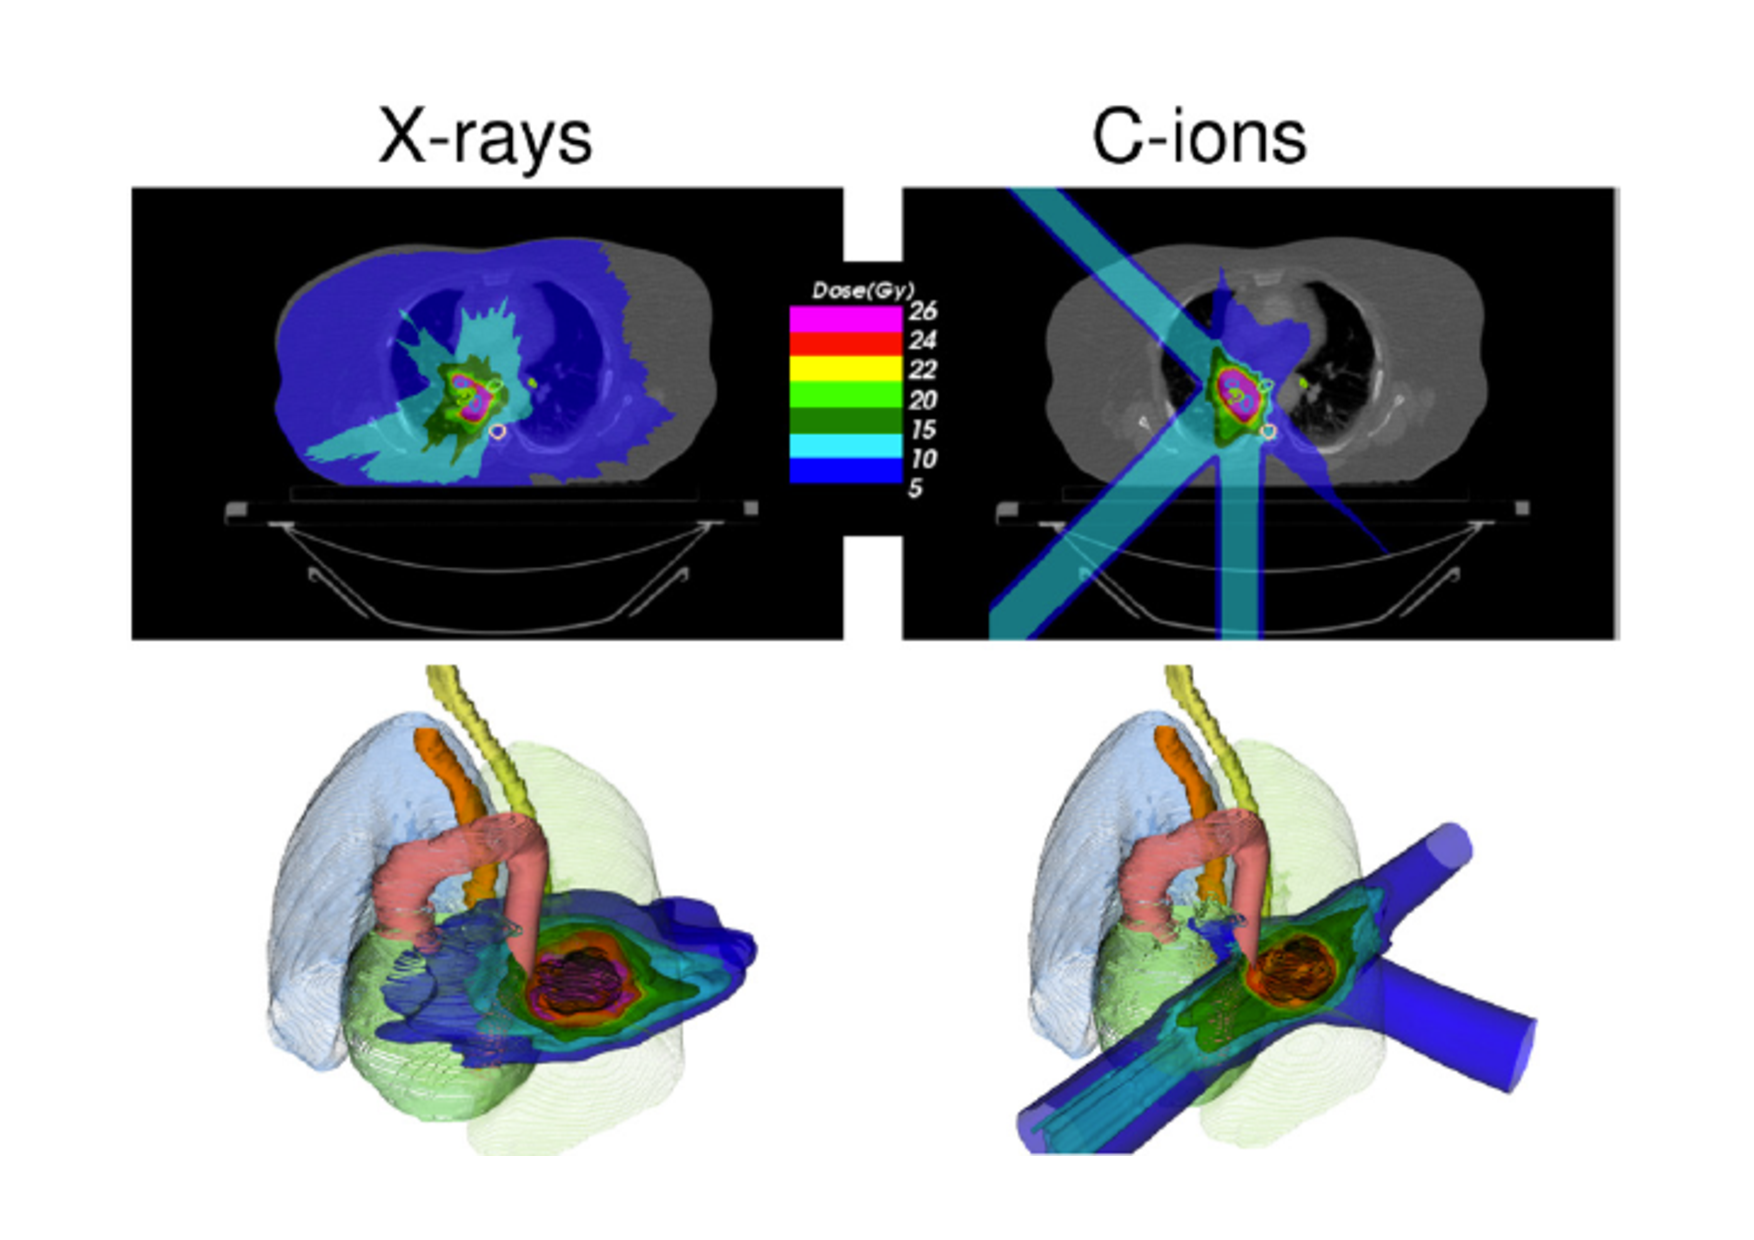
\includegraphics[width=0.8\textwidth]{03_GraphicFiles/chapter1_Introduction/xRayCions_fields.pdf}
\caption{Treatment planning of lung cancer for the irradiation with x-rays (left) or carbon ions (right) (in~\cite{Durante2016}).}
\label{chap1::fig::XraysCionsFields}
\end{figure} 

\begin{figure}[!htbp]
\centering
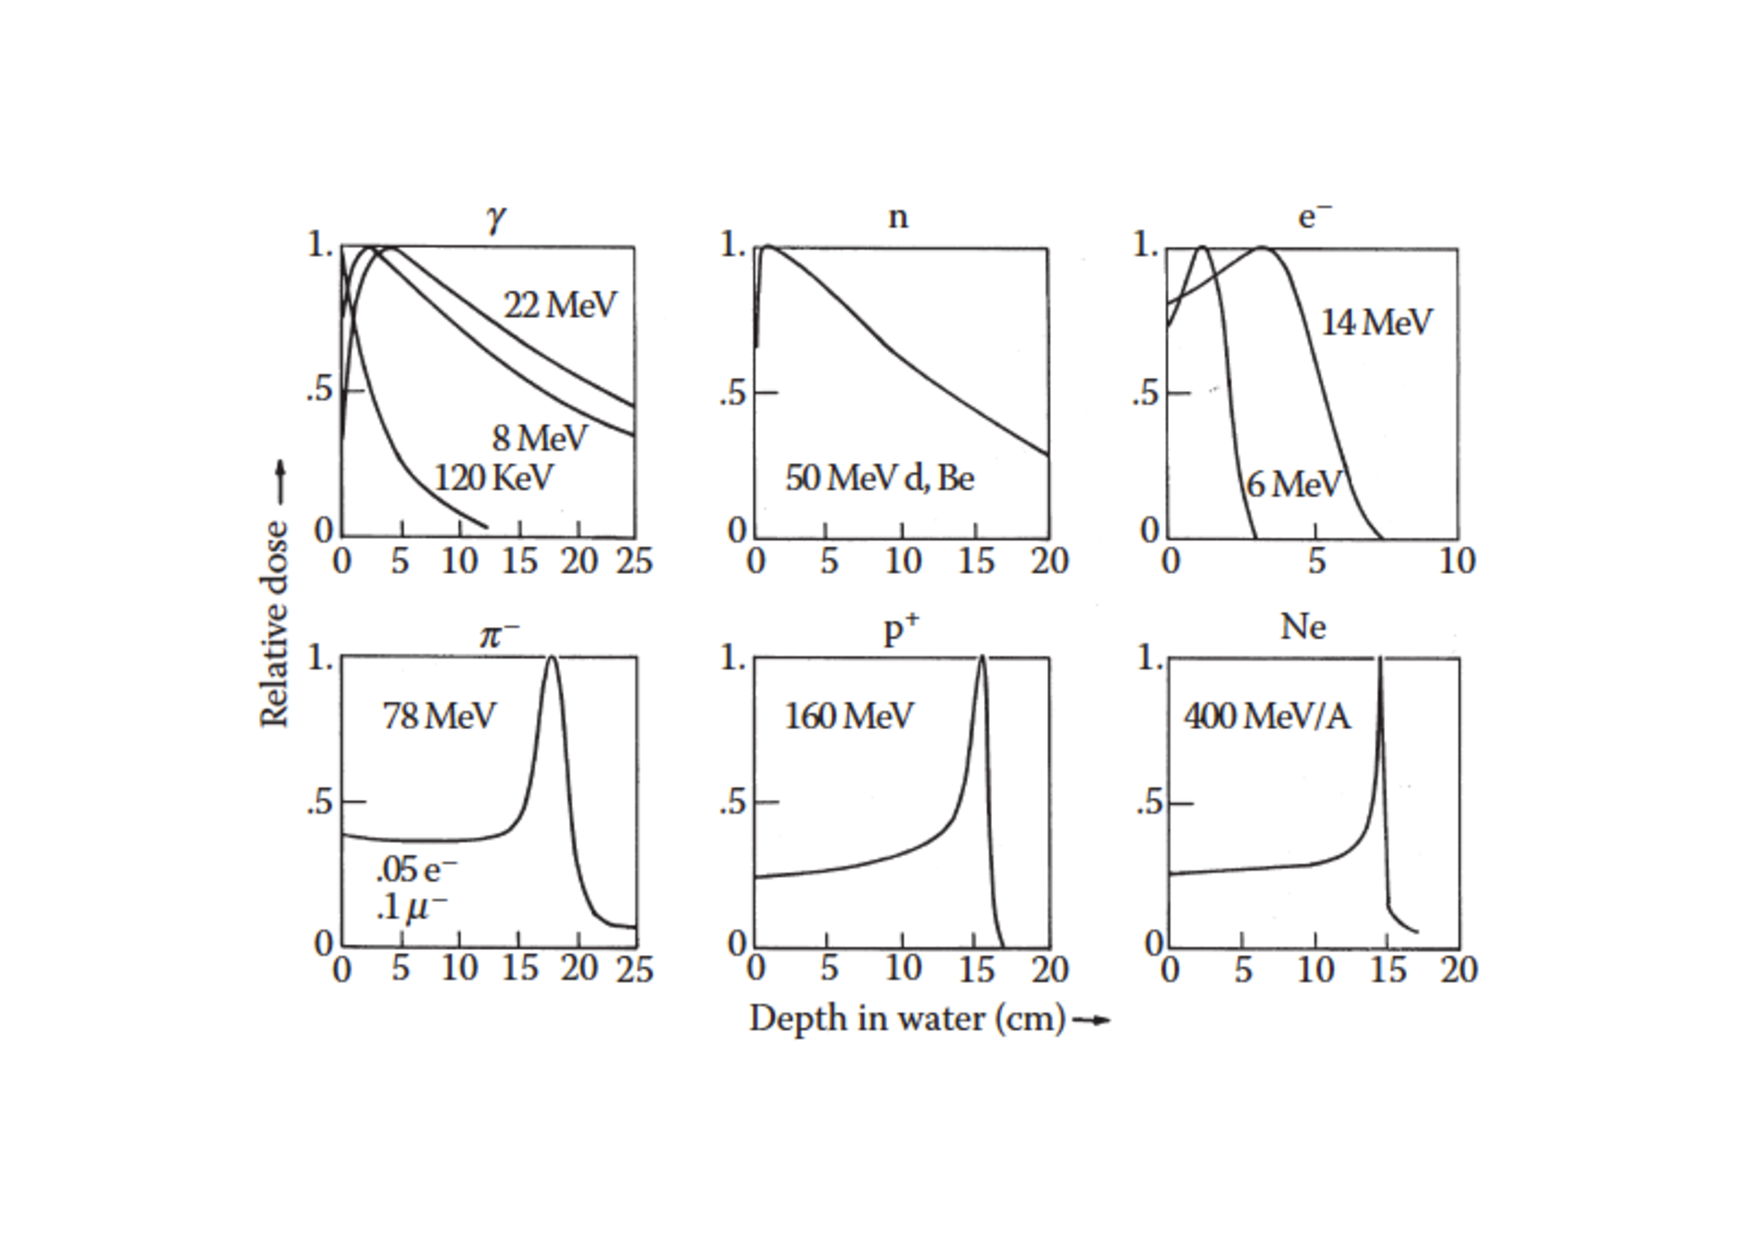
\includegraphics[width=0.9\textwidth , trim={0.5cm 1.5cm 0.5cm 1.5cm}, clip=true]{03_GraphicFiles/chapter1_Introduction/depth_doseProf_multipleIMG.pdf}
\caption{Relative dose as a function of the particle depth in water for different particle species. For photons, the reported energy in MeV corresponds to MV linac-accelerated electron induced bremmstrahlung. In~\cite{PaganettiBook2012}.}
\label{chap1::fig::Depth-doseProf}
\end{figure} 

\subsubsection{Charged particle interactions in matter}\label{chap1::subsubsec::ionInteractions}

The nuclear charged particle interactions in matter can be described by three main mechanisms: \gls{em} inelastic interaction with the atomic electrons, \gls{em} elastic interactions with the atomic nuclei, and nuclear reactions. In addition to the listed interactions, also Bremsstrahlung is theoretically possible, but its effect is negligible at ion energies of clinical interest. 
The \gls{em} inelastic interactions with atomic electrons cause an energy loss which is generally approximated with a \gls{csda} for simplicity, assuming a mono-dimensional quasi-linear ion path and an average, continuous energy loss rate. The mass difference between electrons and ions (as an example, the proton mass is 1832 times greater than that of an electron), justifies the quasi-linear approximation, while the significant cross-section for small energy transfer allows one to consider a continuous decelerating force. The elastic repulsion caused by an atomic nucleus is able to deflect the projectile ion, with an angle which depends on the target-projectile relative mass. The inelastic nuclear reactions are less frequent, but reduce the intensity of the primary beam (the primary particle is destroyed or deflected at large angle), and cause the emission of secondary nuclear fragments. A schematic view of the three main interaction mechanisms described is given in \figurename~\ref{chap1::fig::protInteractions} for the example case of protons, while in the following the effects of these interactions are detailed.   

\begin{figure}[!htbp]
\centering
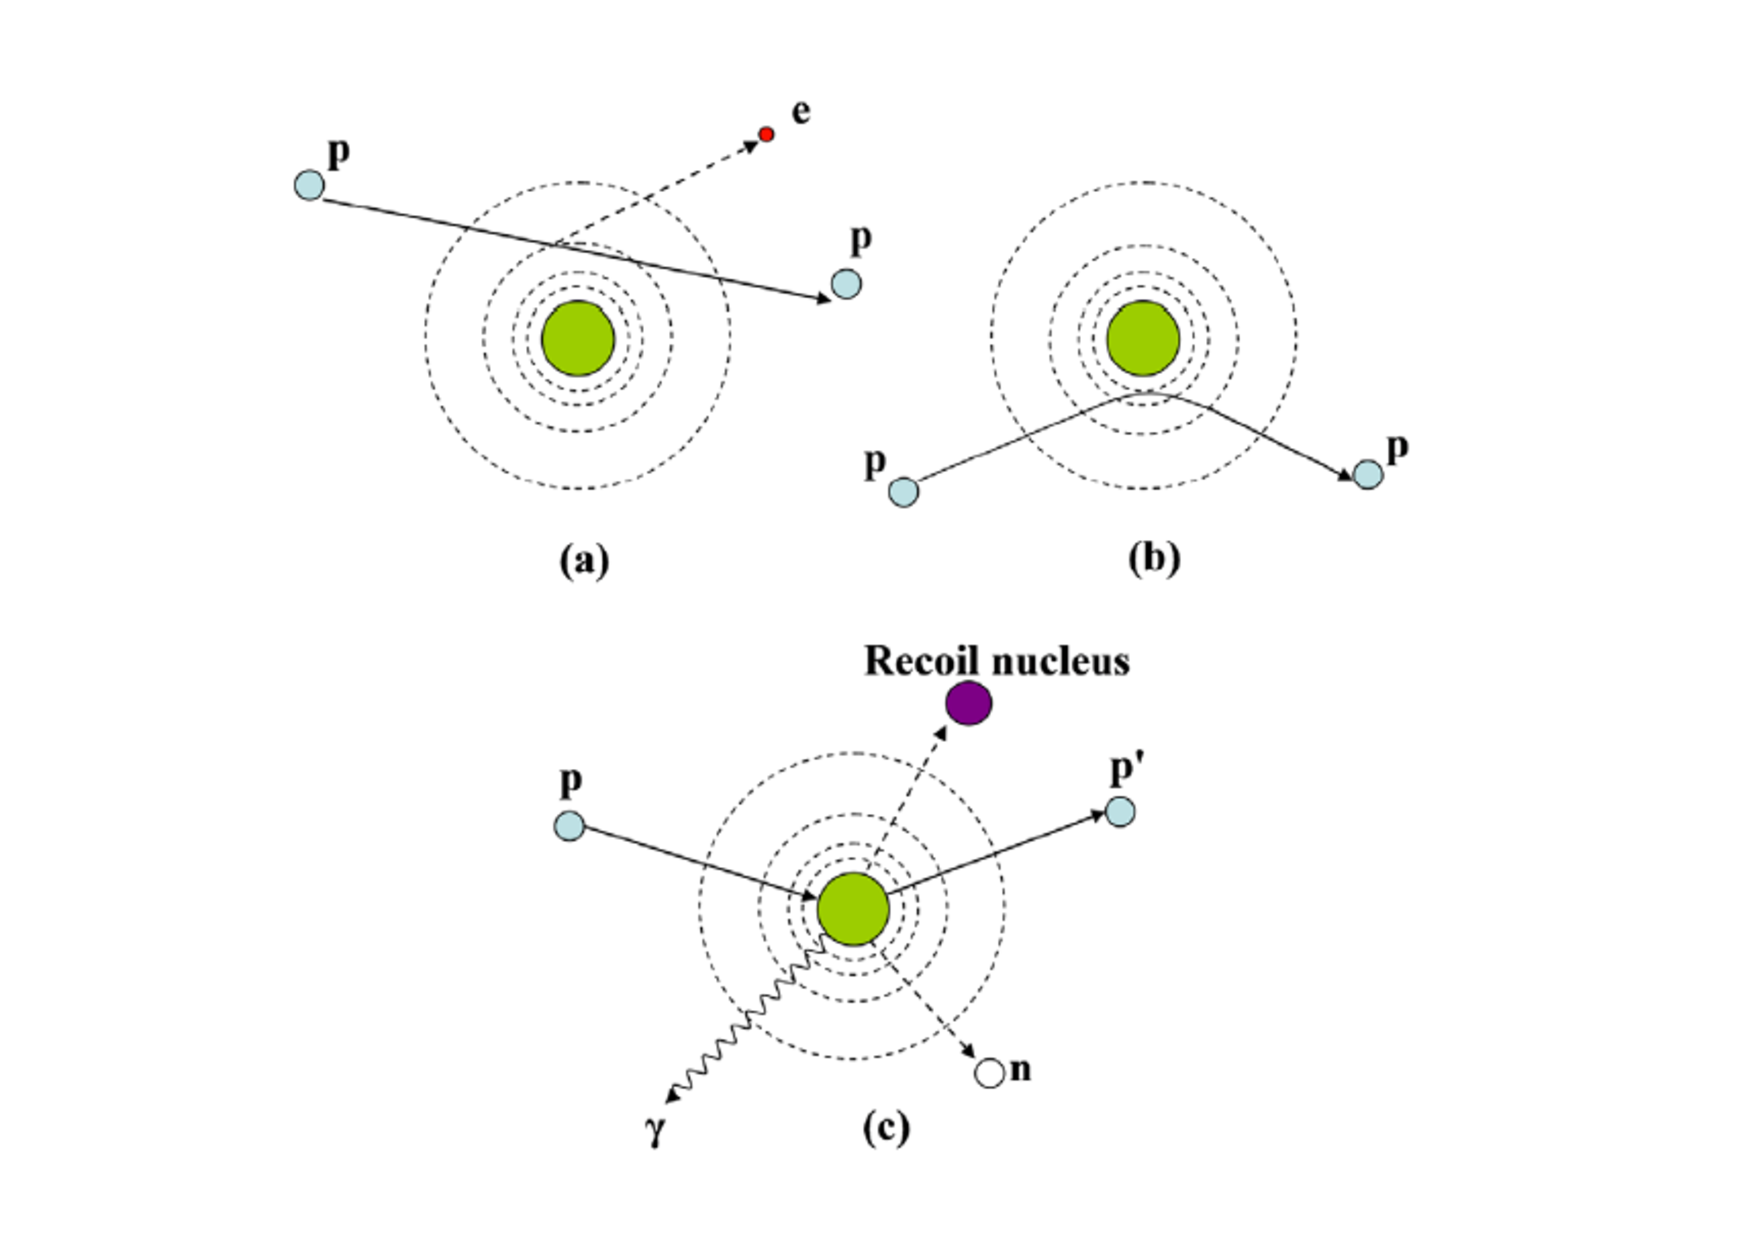
\includegraphics[width=0.8\textwidth]{03_GraphicFiles/chapter1_Introduction/protonInteractions.pdf}
\caption{Schematic view of an example of the three main interactions mechanics of protons in matter: Coulomb interaction with atomic electrons (a), Coulomb interactions with atomic nucleus (b), nuclear reactions(c). In~\cite{Newhauser2015}.}
\label{chap1::fig::protInteractions}
\end{figure} 

At the primary particle velocities of clinical interest,  \myMarginnote{\gls{em} \\ interactions with \\ target atomic electrons} the ion energy loss rate is dominated by inelastic collisions with the target atomic electrons and is well described by the formula attributed to Bethe~\parencite{Bethe1930} and Bloch~\parencite{Bloch1933}, often referred as Bethe-Bloch formula, reported in equation~\ref{chap1::eq::bethe-bloch} in its form independent of the mass density. This expression is also known as mass stopping power.

\begin{equation}
\frac{S}{\rho} = -\frac{\mathrm{d}E}{\rho \mathrm{d}x} = 4\pi N_{A}r^{2}_{e}m_{e}c^{2}\frac{z^{2}}{\beta^{2}}\frac{Z}{A}\bigg[\ln{\frac{2m_{e}c^{2}\beta^{2}\gamma^{2}}{I}}-\beta^{2}-\frac{\delta}{2}-\frac{C}{Z}\bigg]
\label{chap1::eq::bethe-bloch}
\end{equation}

where $N_{A}$ is the Avogadro's number (6.022 $\times$10$^{23}$mol$^{-1}$), $r_{e}$ is the classical electron radius expressed in equation~\ref{chap1::eq::electronRad} with $\epsilon_{0}$ = 8.854 $\times$ 10$^{-12}$~F/m the permittivity of the vacuum, $m_{e}c^{2}$ = 511~keV the mass energy of the electron, $e$ = 1.6 $\times$ 10$^{-19}$~C the electron charge and $c$ the speed of light,  

\begin{equation}
r_{e} = \frac{1}{4\pi\epsilon_{0}}\frac{e^2}{m_{e}c^{2}} = \mathrm{2.181\times10^{-15} m}
\label{chap1::eq::electronRad}
\end{equation}

$z$ is the charge of the projectile, $Z$ and $A$ are the atomic number and mass of the target material, respectively, $\beta = v/c$ is the projectile velocity, $\gamma = (1-\beta^{2})^{-1/2}$, $I$ is the mean excitation potential of the target material. The last two terms represent corrections for high energies ($\delta$ density effect correction term) and low energies ($C$ shell correction term) incident ions. By observing equation~\ref{chap1::eq::bethe-bloch}, it clearly emerges how the energy loss rate is proportional to the square of charge and inverse velocity of the projectile. The target material composition also plays a major role. As the logarithmic term varies slowly with the target properties, and since Z/A is also almost constant, it turns that the linear energy loss rate is proportional to the electron density, and thus to the atomic density (to be noticed, for clinical applications, that the density in a patient can vary by almost three orders of magnitude, ranging from the air cavity in the lungs to the most dense bones). 
As already mentioned, the energy loss increases for decreasing ion energy due to the $1/\beta^{2}$ dependence at high velocities (when the projectile velocity is much larger than its orbital electron velocities, and therefore remains fully stripped), and the maximum energy-loss rate, corresponding to the Bragg peak depth, is reached at the projectile velocity expresses as

\begin{equation}
v_p = z^{2/3}v_{0}
\label{chap1::eq::maxEloss}
\end{equation}

where $v_{0} = e^2/\hslash$ is the Bohr velocity ($\beta$ = 1/137). For velocity values below $v_p$, corresponding to the average orbital velocity in the Thomas-Fermi atomic model, the ion captures electrons and its charge decreases, as well as the stopping force. However, the residual range is small (a few tens micrometers), and therefore the Bragg peak is assimilated to the end of the ion path. Note that, at very small velocities, atomic elastic collisions become important in the slowing down process. 

The energy loss rate equation directly leads \myMarginnote{Ion range} to the definition of the ion beam range in matter (if we neglect nuclear interactions which cause a modification of the projectile nature), which is the integral over the incident energy of the energy loss per track unit, reported in equation~\ref{chap1::eq::rangeIntegral}. This formulation assumes a 1D ion trajectory with negligible lateral scattering (mentioned above and discussed below) and uses the \gls{csda}. 

\begin{equation}
R(E) = \int_{0}^{E}(\frac{\mathrm{d}E'}{\mathrm{d}x})^{-1}\mathrm{d}E' 
\label{chap1::eq::rangeIntegral}
\end{equation}

where E is the ion beam incident energy. To be noticed that the range is not a deterministic value, but it is intended as an average value and defined for the whole beam, not for single incident particles, which are affected by statistical fluctuations in the energy loss, leading to the so-called \enquote{range straggling} (described by different theoretical models, such as the ones in~\cite{Bohr1915, Landau1944, Vavilov1957}, and detailed below). The integration of the Bethe-Bloch is often a hard task, but, as realized by Bragg and Kleeman~\parencite{Bragg1905}, the range dependence on the incident particle energy can be practically expressed with an analytic approach as the power law in equation~\ref{chap1::eq::rangePowerLaw}. This approximation directly derives from studies on alpha particles which anticipated the formulation of equation~\ref{chap1::eq::bethe-bloch}.

\begin{equation}
R(E) = \alpha E^{p}
\label{chap1::eq::rangePowerLaw}
\end{equation}

where E is again the ion beam initial energy, the constant $\alpha$ depends on the target material and the constant $p$ is related to the projectile energy (or velocity). The proton range can be easily scaled to other ions at the same energy per nucleon in the same material with a factor $M/z^{2}$, where $M$ is the ion mass. The range of ions with the same specific energy scales from water to other homogeneous material with a factor of $A/Z^{2}$.
%An empirical expression has been derived to scale the proton calculated range to heavier ions at the same energy per nucleon in the same material: it is reported in equation~\ref{chap1::eq::ScaleRange}.

%\begin{equation}
%\frac{R_{2}}{R_{1}} = \frac{M_{2}}{M_{1}}\frac{z_{1}^{2}}{z_{2}^{2}}
%\label{chap1::eq::ScaleRange}
%\end{equation}

%with M and z the ion mass and charge, respectively. Equivalently, for the same particle in different material, the scaling formula is reported in equation~\ref{chap1::eq::ScaleRangeMat}.

%\begin{equation}
%\frac{R_{2}}{R_{1}} = \frac{\rho_{2}}{\rho_{1}}\frac{\sqrt{A_{1}}}{\sqrt{A_{2}}}
%\label{chap1::eq::ScaleRangeMat}
%\end{equation}
 
% with $\rho$ and $A$ density and atomic mass of the target material, respectively.
 
The ion range predicted by equations~\ref{chap1::eq::rangeIntegral} or~\ref{chap1::eq::rangePowerLaw} \myMarginnote{Range straggling} is an average value, calculated by considering a smooth and continuous energy loss process and neglecting the individual ion behavior. The actual range suffers from statistical fluctuations in the projectile energy loss that broaden the Bragg peak, in the so-called \enquote{range straggling}. In general, the longitudinal beam straggling can be described by an asymmetric distribution~\parencite{Vavilov1957}, which is approximated to a Gaussian in the limit of many collisions, leading to the expression of the relative straggling in equation~\ref{chap1::eq::relStragg}:
 
 \begin{equation}
\frac{\sigma_{R}}{R} = (M^{-\frac{1}{2}})\phi\frac{E}{Mc^{2}}
\label{chap1::eq::relStragg}
\end{equation}

The ratio of the straggling width $\sigma_{R}$ and mean range $R$ is then all the more reduced as the ion mass ($M$) increases, with $\phi$ a slowly varying function which depends on the target material~\parencite{Rossi1952} and E the ion energy. According to equation~\ref{chap1::eq::relStragg}, it is interesting to notice how the relative straggling for carbon ions is about 3.5 times smaller with respect to protons (e.g. 7~mm and 25~mm at 18~cm of average range for carbon ions and protons, respectively - see~\cite{Durante2016}). In addition to energy loss fluctuations, range straggling contributions also come from the beam initial energy distribution: the actual beam is not perfectly mono-energetic, and the energy distribution width is determined by the accelerator and the beam optics elements. This contribution has to be added (quadratic sum) to the range straggling estimate. Figures~\ref{chap1::fig::TailBragg_p} and~\ref{chap1::fig::TailBragg} show the depth-dose profiles of proton and carbon ion mono-energetic beams, respectively, at different energies in water. The effect of range straggling is clearly visible in the broadening of the Bragg peak, which is more significant for protons with respect to carbon ions, and increases for increasing range in matter.  

In addition to the energy loss process considered till here,  \myMarginnote{\gls{em} \\ interactions with \\ target nuclei} which shapes the beam in the longitudinal direction (range variations), the actual delivered dose also depends on the lateral beam profile, which derives from the size and angular divergence of the incident beam and is mainly governed, at the target level, by elastic Coulomb scattering with atomic nuclei and by secondary particles produced by nuclear fragmentation. 
In case an ion passes close to a target atomic nucleus, it is elastically scattered by the repulsive electromagnetic force: the projectile loses a negligible amount of energy, so that this kind of interaction can be neglected when calculating the energy loss rate described above, but the change in its trajectory must be estimated for range and dose predictions. %The \gls{mcs} is determined by elastic electromagnetic interactions of the beam ions with the target nuclei, causing considerable deflections in the single ion trajectory which mainly affect the lateral beam profile causing a spread. 
Starting from the single scattering model by Rutherford~\parencite{Rutherford1911}, and moving to the calculation of the statistical distribution function for the scattering angle at a certain penetration depth given by~\cite{Bothe1921}, a complete theory allowing for the calculation of the scattering angle probability in case of \gls{mcs} has been proposed by Moli\`{e}re~\parencite{Moliere1948} (confirmed to provide good predictions thanks to a large set of proton beam spread data - see~\cite{Gottschalk1993}). More practical formulas were then derived afterwards (see~\cite{Lewis1950, Highland1975, Gottschalk2010}). The Moli\`{e}re formulation has been then simplified for analytic calculations towards a Gaussian approximation. The Gaussian standard deviation ($\sigma_{\theta}$) expression in equation~\ref{chap1::eq::latSpread} is given by the characteristics \gls{mcs} angle $\theta$~\parencite{Highland1975}

\begin{equation}
\sigma_{\theta} = \frac{14.1 \mathrm{MeV}}{\beta p c}Z_{p}\sqrt{\frac{L}{L_\mathrm{rad}}}\big[1+0.038 \ln\big(\frac{L}{L_{\mathrm{rad}}}\big) \big]
\label{chap1::eq::latSpread}
\end{equation}

where $\beta$, $p$ and $Z_{p}$ are respectively the projectile velocity, momentum and charge, $c$ is the speed of light,  $L$ is the material thickness and $L_{\mathrm{rad}}$ is the radiation length (reported for common materials in~\cite{Tsai1974}) expressed in equation~\ref{chap1::eq::radL}. 

\begin{equation}
L_{\mathrm{rad}} = \frac{716.4}{Z(Z+1)ln(\frac{287}{\sqrt{Z}})} \, \mathrm{g / cm^{3}}
\label{chap1::eq::radL}
\end{equation}
with $Z$ the atomic number of the material.
Even if the Gaussian approach is not always accurate to describe the lateral beam spread (mainly at large angles), the Moli\`{e}re \gls{mcs} description allows to retrieve the main parameters contributing to this effect: in particular, heavier particles have narrower lateral beam spread, and the scattering effect increases at increasing ion range (but is inversely proportional to the beam energy) and for high-Z materials. A more precise model of the lateral beam spread should involve nuclear reactions and the produced secondary particles, but an analytic approach is difficult and Monte Carlo based calculations are necessary, but still time consuming. The empirical parameterizations are still strongly based on experimental data: as an example, measurements of the lateral beam spread in a water column for different beam energies (ranges) are reported in~\cite{Pedroni2005}. In~\figurename~\ref{chap1::fig::latSpread} the lateral spread of different ions in water is plotted as a function of range for various beam energies (A) and as a function of beam energy (B) after 15~cm range in water.

\begin{figure}[!htbp]
\centering
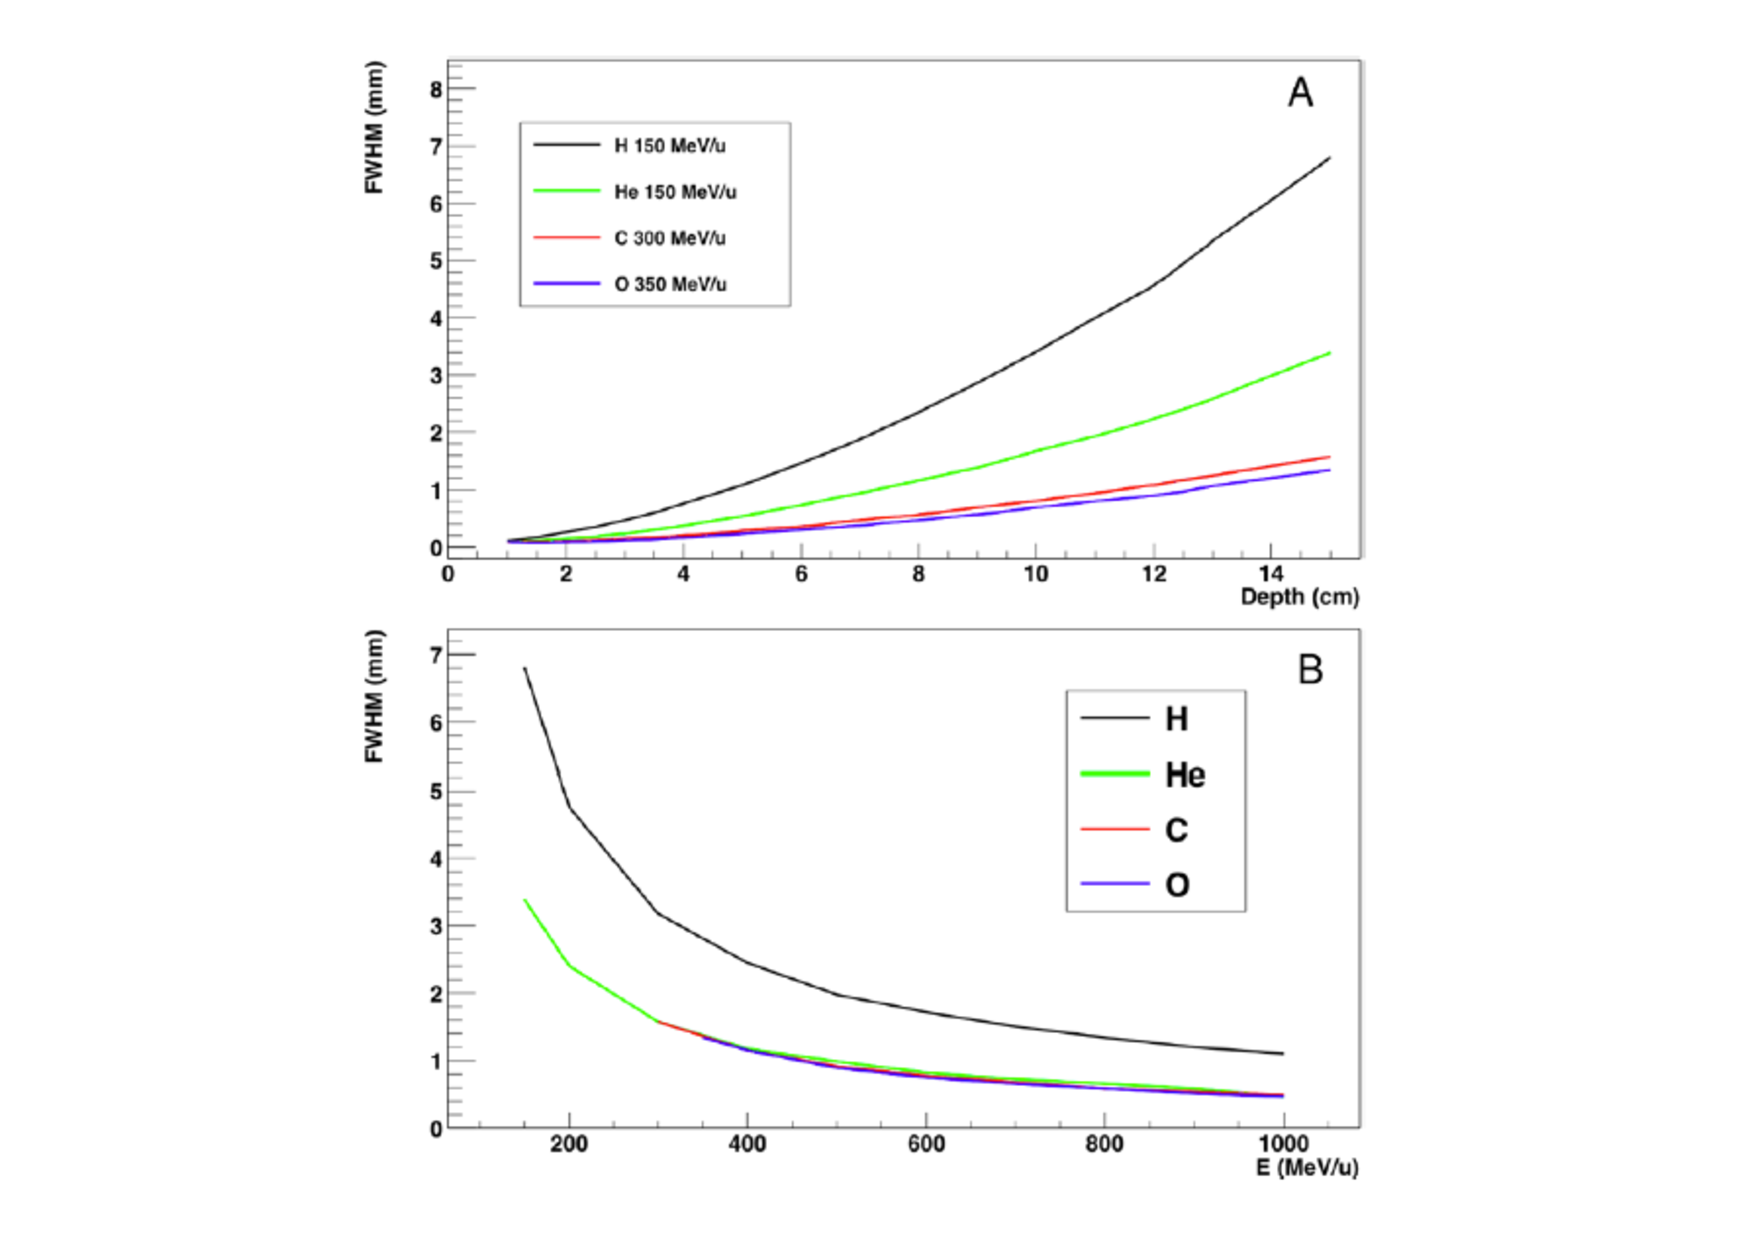
\includegraphics[width=0.8\textwidth]{03_GraphicFiles/chapter1_Introduction/lateralSpread.pdf}
\caption{Lateral spread of different ions in water obtained with Geant4 Monte Carlo simulations. The \gls{fwhm} of the beam spot distribution is presented as a function of depth in water (A) for beams at different energies and as a function of beam energy (B) after 15~cm range in water. In~\cite{Durante2016}.}
\label{chap1::fig::latSpread}
\end{figure}   

In addition to the electromagnetic interactions with electrons and nuclei \myMarginnote{Nuclear reactions}  which mainly govern the stopping process, primary ions impinging on a target also undergo nuclear reactions with the target nuclei which may cause the disintegration of the projectile and the target nucleus or a partial fragmentation. In general, nuclear reactions induce modifications in the beam composition and cause variations in the longitudinal and lateral beam structure which must be taken into account for the delivered physical and biological dose estimate. Moreover, this kind of reactions leads to the production of secondary particles, such as secondary protons, neutrons, hydrogen and helium isotopes and other ions (mainly with heavy ion irradiation), and gammas.
In the high velocity regime (when the relative velocity in the nuclei center of mass is much larger than the nucleon Fermi velocity), the nuclear interactions occurring between projectile ions and target nuclei can be described by a two-step process. At the \enquote{collision} stage, depending on the distance between projectile and target centers (impact parameter $b$), a variable number of nucleons is involved in the interaction and composes the reaction zone generally defined as \enquote{fireball}. The so-called \enquote{spectator} nucleons are almost not affected and create projectile-like and target-like fragments (\enquote{fragmentation} process), often in excited states. After the collision, the excited fireball and fragments decay through the emission of secondary light particles, in the so-called \enquote{de-excitation} process, and the lighter fragments continue their path through the target. A schematic view of a typical nuclear reaction is given in \figurename~\ref{chap1::fig::nuclReac}. 
Several models have been proposed to describe the nuclear interactions in its two steps. The \gls{inc} model has been originally proposed by Serber and Heisenberg~\parencite{Serber1947}, and later implemented in the sixties~\parencite{Bertini1974}, and is used to describe the collision stage. It is based on a series of two-body interactions between the incident particle and the target nucleons, which are considered quasi-free. For each nuclear interaction, the code models the complete outcome, and all produced particles are tracked until they are below a given energy threshold, in a process called \enquote{intra-nuclear cascade}. Other candidates are the \gls{qmd}, which describes each nucleon as a gaussian wave packet, and all nucleons are included in the collision, and the \gls{bme}, which is a sophisticated model describing the thermalization of composite nuclei for low energy projectiles. The de-excitation stage can involve the so-called \enquote{evaporation}~\parencite{Weisskopf1937}, where light fragments are emitted from the excited nuclei, \enquote{fission} of the excited nuclei in two fragments (for high-Z nuclei which can be only found in implants), \enquote{Fermi-breakup} of light nuclei which disassembles in smaller fragments~\parencite{Fermi1950}, and gamma emission to dissipate the residual energy. 
The majority of the complete models for nucleus-nucleus reactions includes the previously described ones (often in simplified versions, optimized in order to minimize the calculation time) and is a variant of the so-called \enquote{abrasion-ablation} model~\parencite{Hufner1975}, generally used in transport codes. The abrasion phase describes the collision and the ablation one models the de-excitation stage; to be noticed that the ablation description is generally more adapted to peripheral collisions (high $b$), where the fragments are excited after the collision and decay to the ground state by emitting light particles and gamma rays. 

\begin{figure}[!htbp]
\centering
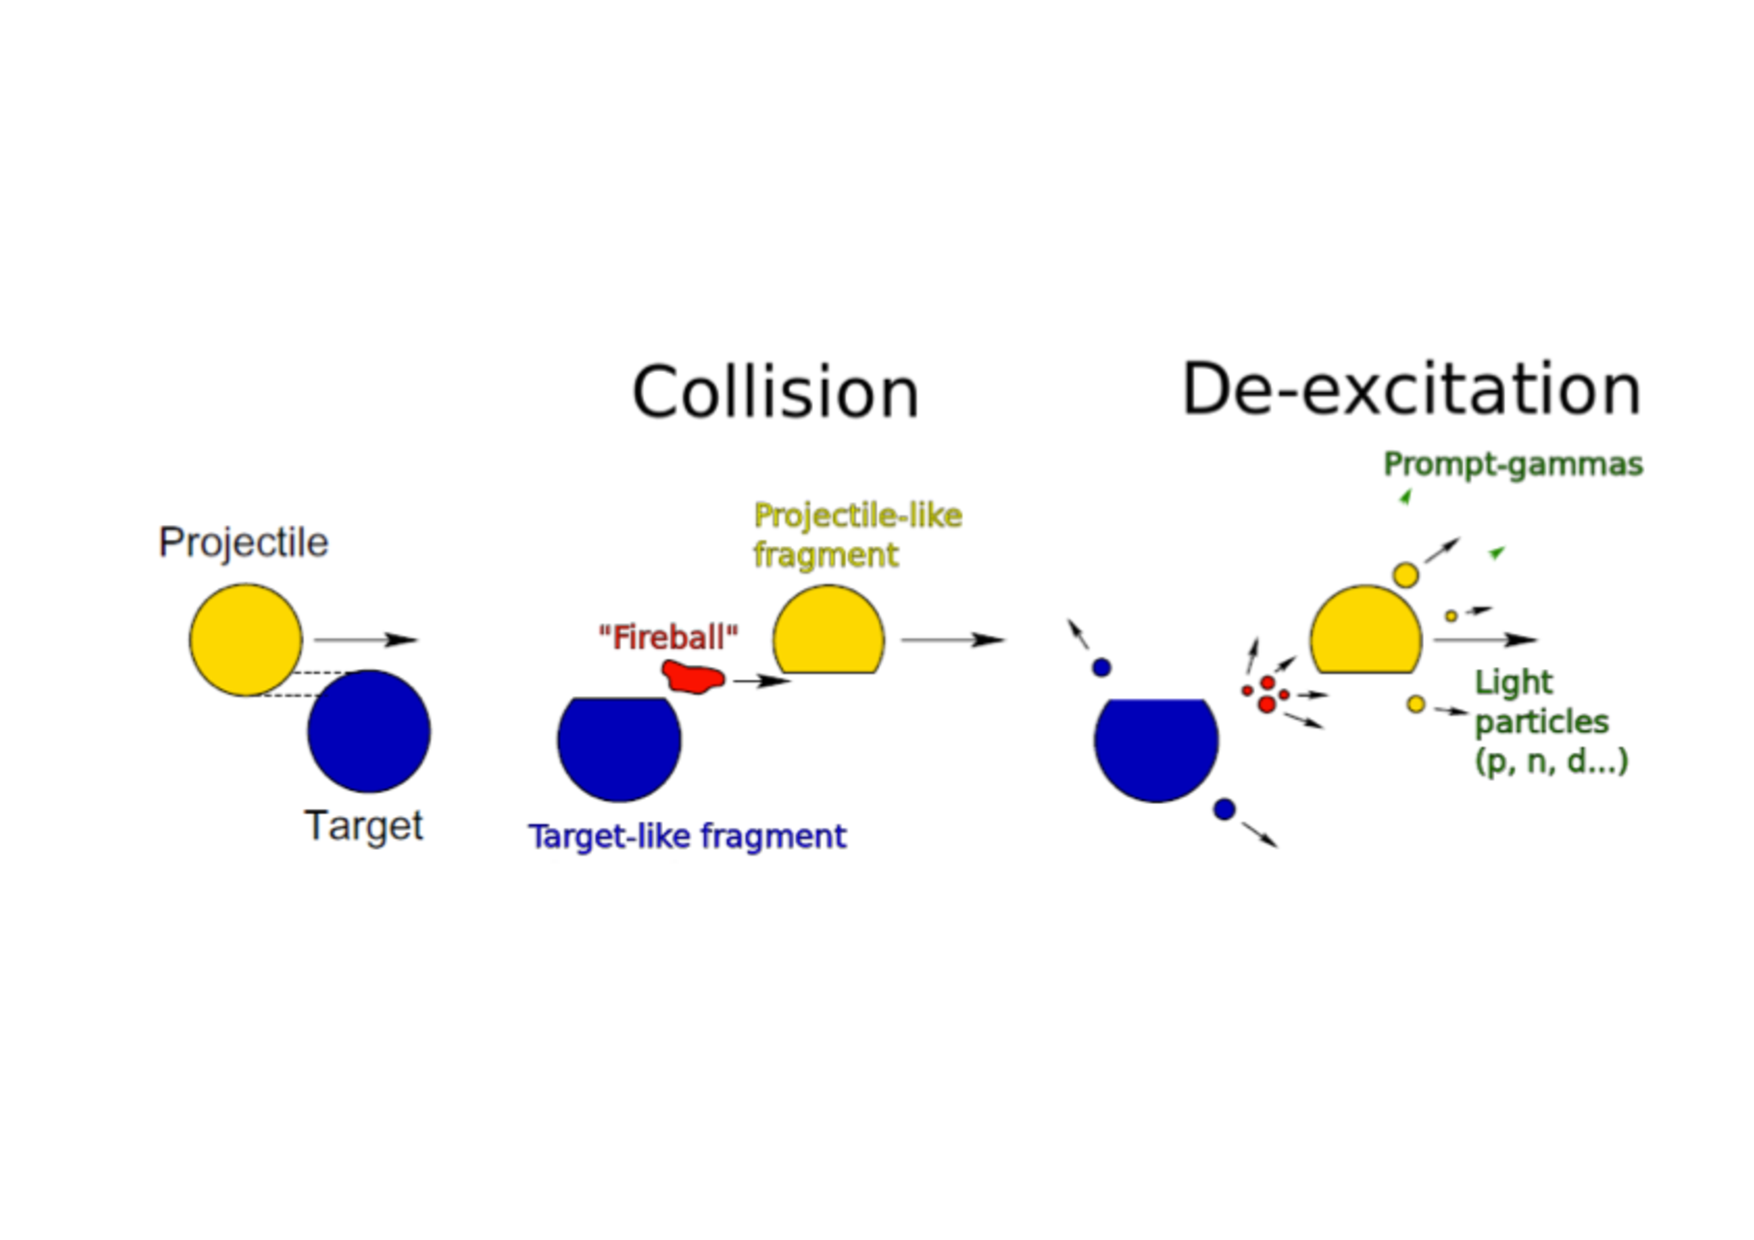
\includegraphics[trim={0 5cm 0 3cm} , clip , width=0.95\textwidth]{03_GraphicFiles/chapter1_Introduction/nuclReactionsScheme.pdf}
\caption{Schematic view of the nuclear reaction between a projectile and a target nucleus. The two steps are defined as \enquote{collision} and \enquote{de-excitation} processes.}
\label{chap1::fig::nuclReac}
\end{figure} 

%, depicted in \figurename~\ref{chap1::fig::abrAbl}.
%\begin{figure}[!htbp]
%\centering
%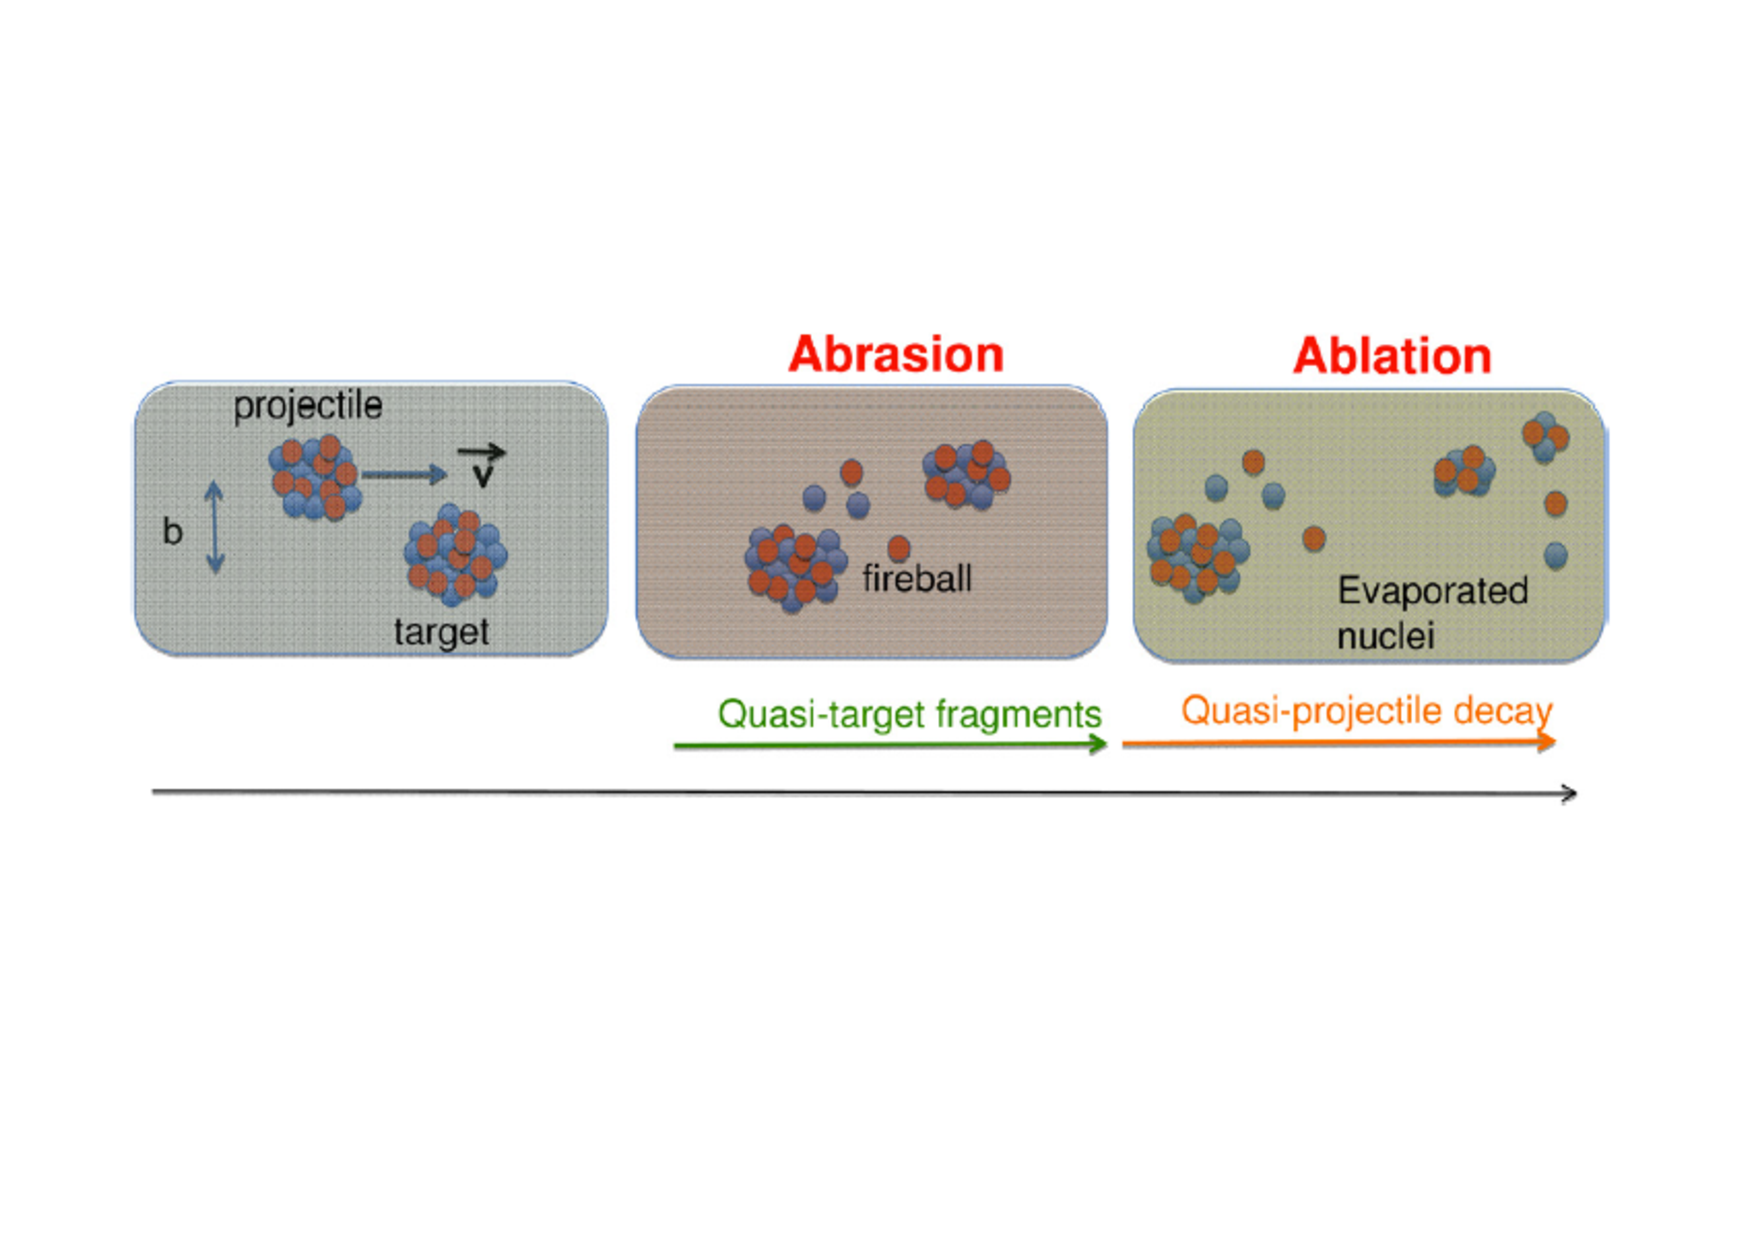
\includegraphics[trim={0 5cm 0 3cm} , clip , width=0.95\textwidth]{03_GraphicFiles/chapter1_Introduction/AbrasionAblation.pdf}
%\caption{Schematic view of the abrasion-ablation model for the description of ion-nucleus interactions (in~\cite{Durante2016}): b is the impact parameter, v is the projectile velocity.}
%%\end{figure} 

Two main effects of fragmentation processes are relevant to ion beam therapy. 
First, the described nuclear reactions cause a loss of primary beam particles; this effect is all the more important for increasing penetration depth. It is clear that in peripheral collisions (high $b$) the probability of primary ion loss is lower with respect to central collisions (small $b$), where projectile and target are most likely completely destroyed. Figures~\ref{chap1::fig::nuclearReacLoss} and~\ref{chap1::fig::nuclearReacLoss_Cion} (top panel) show the primary particle fluence loss in a proton  and carbon ion beam, respectively, as a function of the depth in water. In the entrance region before the falloff the fluence loss is caused by nuclear reactions, while close to the Bragg peak the fluence falloff is mainly due to stopping of primary particles with zero residual energy. In addition, the range straggling effect is visible. Concerning carbon ion beams, as reported in~\cite{Durante2016}, during a standard treatment only 50\% of the primary ions reach the Bragg peak region for $\sim$20~cm range, while the others undergo fragmentation processes and are lost.
Second, lower-mass and Z fragments result from the nuclear interactions in case of irradiation with ions heavier than protons (with proton beams, only secondary protons and neutrons are produced).
The projectile velocity determines the velocity of the secondary fragments, which can travel with longer ranges with respect to the primaries due to their reduced mass and charge (remember the range scaling factor $M/z^{2}$): this produces a tail in the dose distribution (for ions heavier than protons). The features of this tail have been deeply studied for different primary ions species ($^{10}$B, $^{12}$C, $^{14}$N, $^{16}$O, $^{20}$Ne), and shell-structure effects have been verified with a non-direct relationship between proton number Z and tails extension~\parencite{Schall1996}.  \figurename~\ref{chap1::fig::TailBragg} (and \figurename~\ref{chap1::fig::nuclearReacLoss_Cion}, bottom panel) shows the effects of nuclear reactions on the Bragg curves related to carbon ion beams at different energies stopping in water, measured in a water column~\parencite{Schardt2008}. With increasing primary energy and, consequently, beam penetration depth, the ratio between Bragg peak and entrance plateau dose is reduced by the decreased number of primary ions (this effect is also visible for proton beams in \figurename~\ref{chap1::fig::TailBragg_p}), while the tail after the Bragg peak is wider due to the increased number of lower-Z fragments traveling with longer range. In addition to this, the energy loss stochastic fluctuations are clearly visible in the broadening of the Bragg peak, as already described.  

\begin{figure}
\begin{subfigure}[t]{.49\textwidth}
\hspace{-1cm} 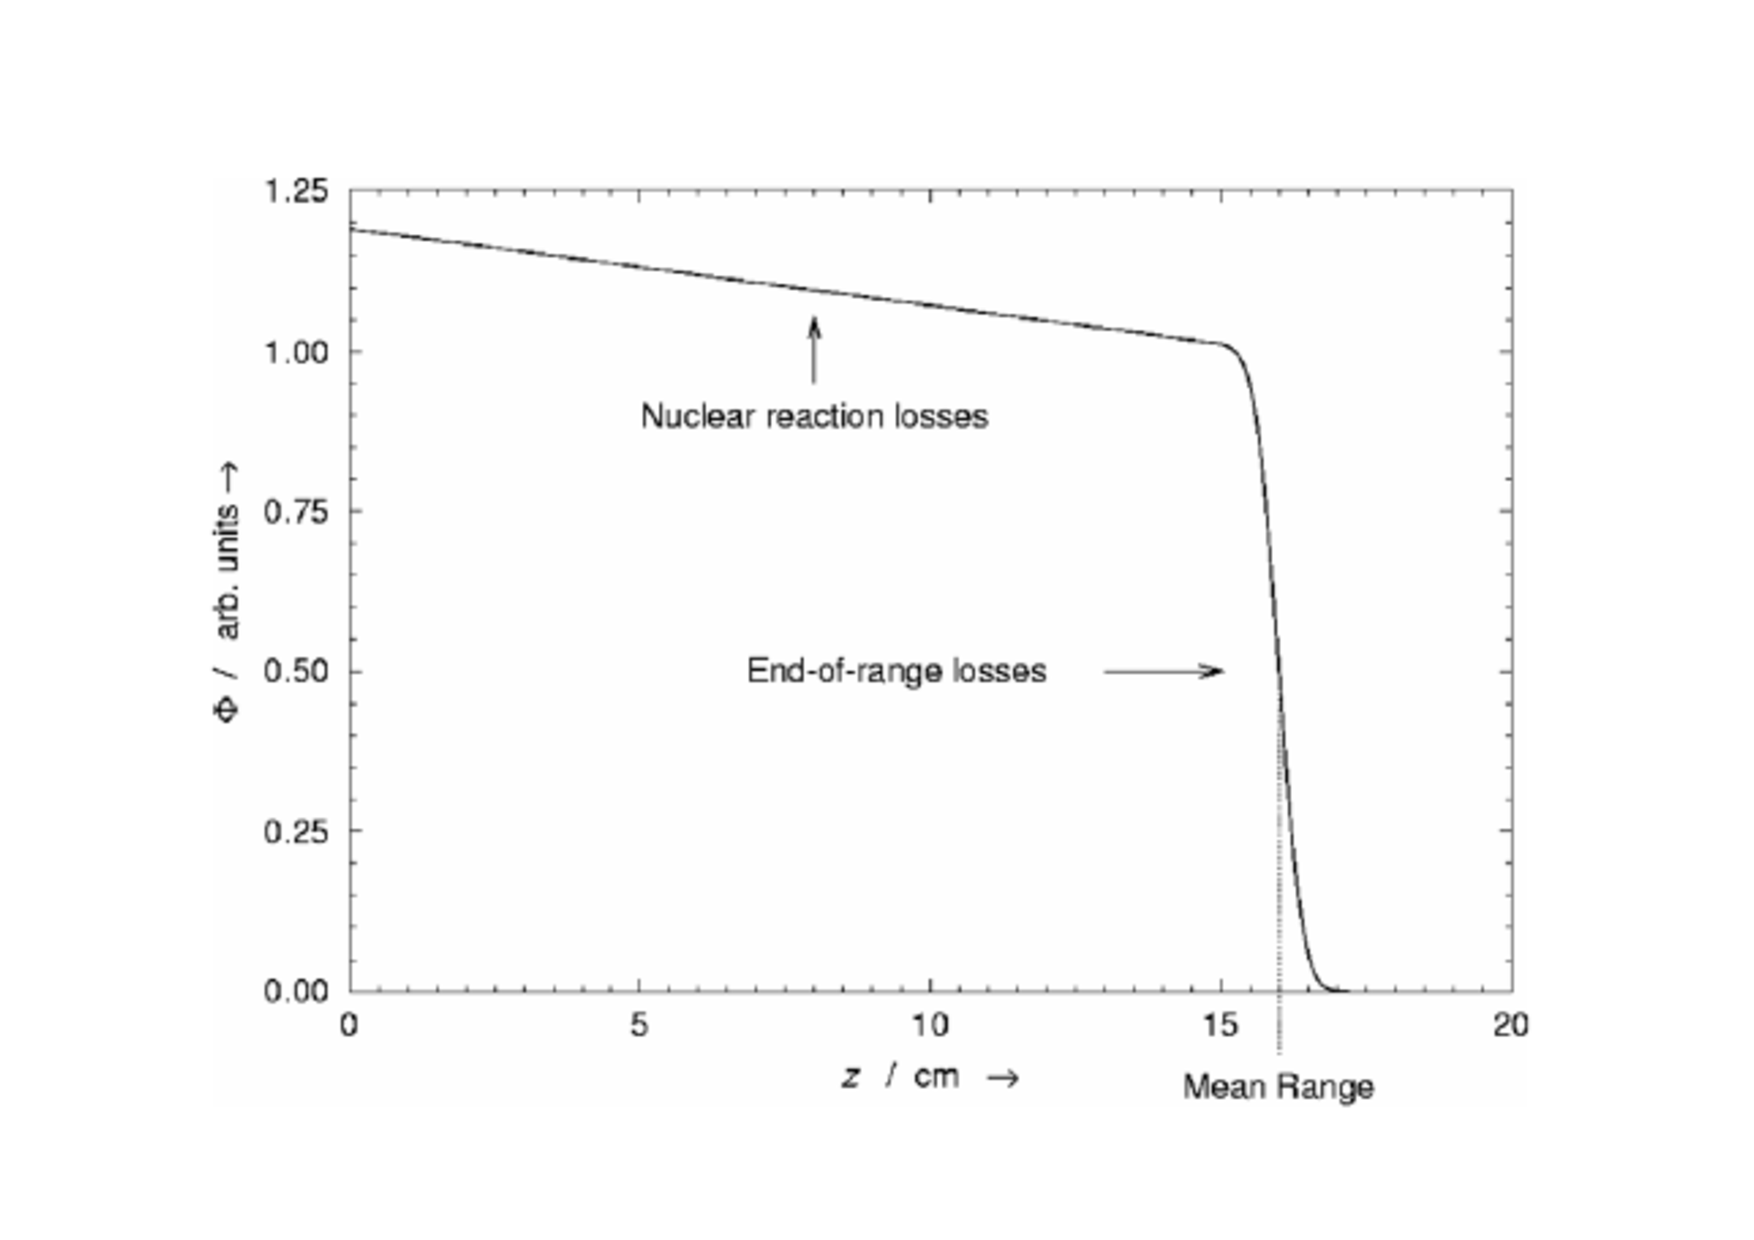
\includegraphics[width=1.2\linewidth]{03_GraphicFiles/chapter1_Introduction/primaryLoss.pdf}
\caption{Primary particle fluence loss in a pro\-ton beam as a function of the depth in water. In~\cite{Newhauser2015}.}
\label{chap1::fig::nuclearReacLoss}
\end{subfigure}
\begin{subfigure}[t]{.49\textwidth}
\hspace{-1cm} 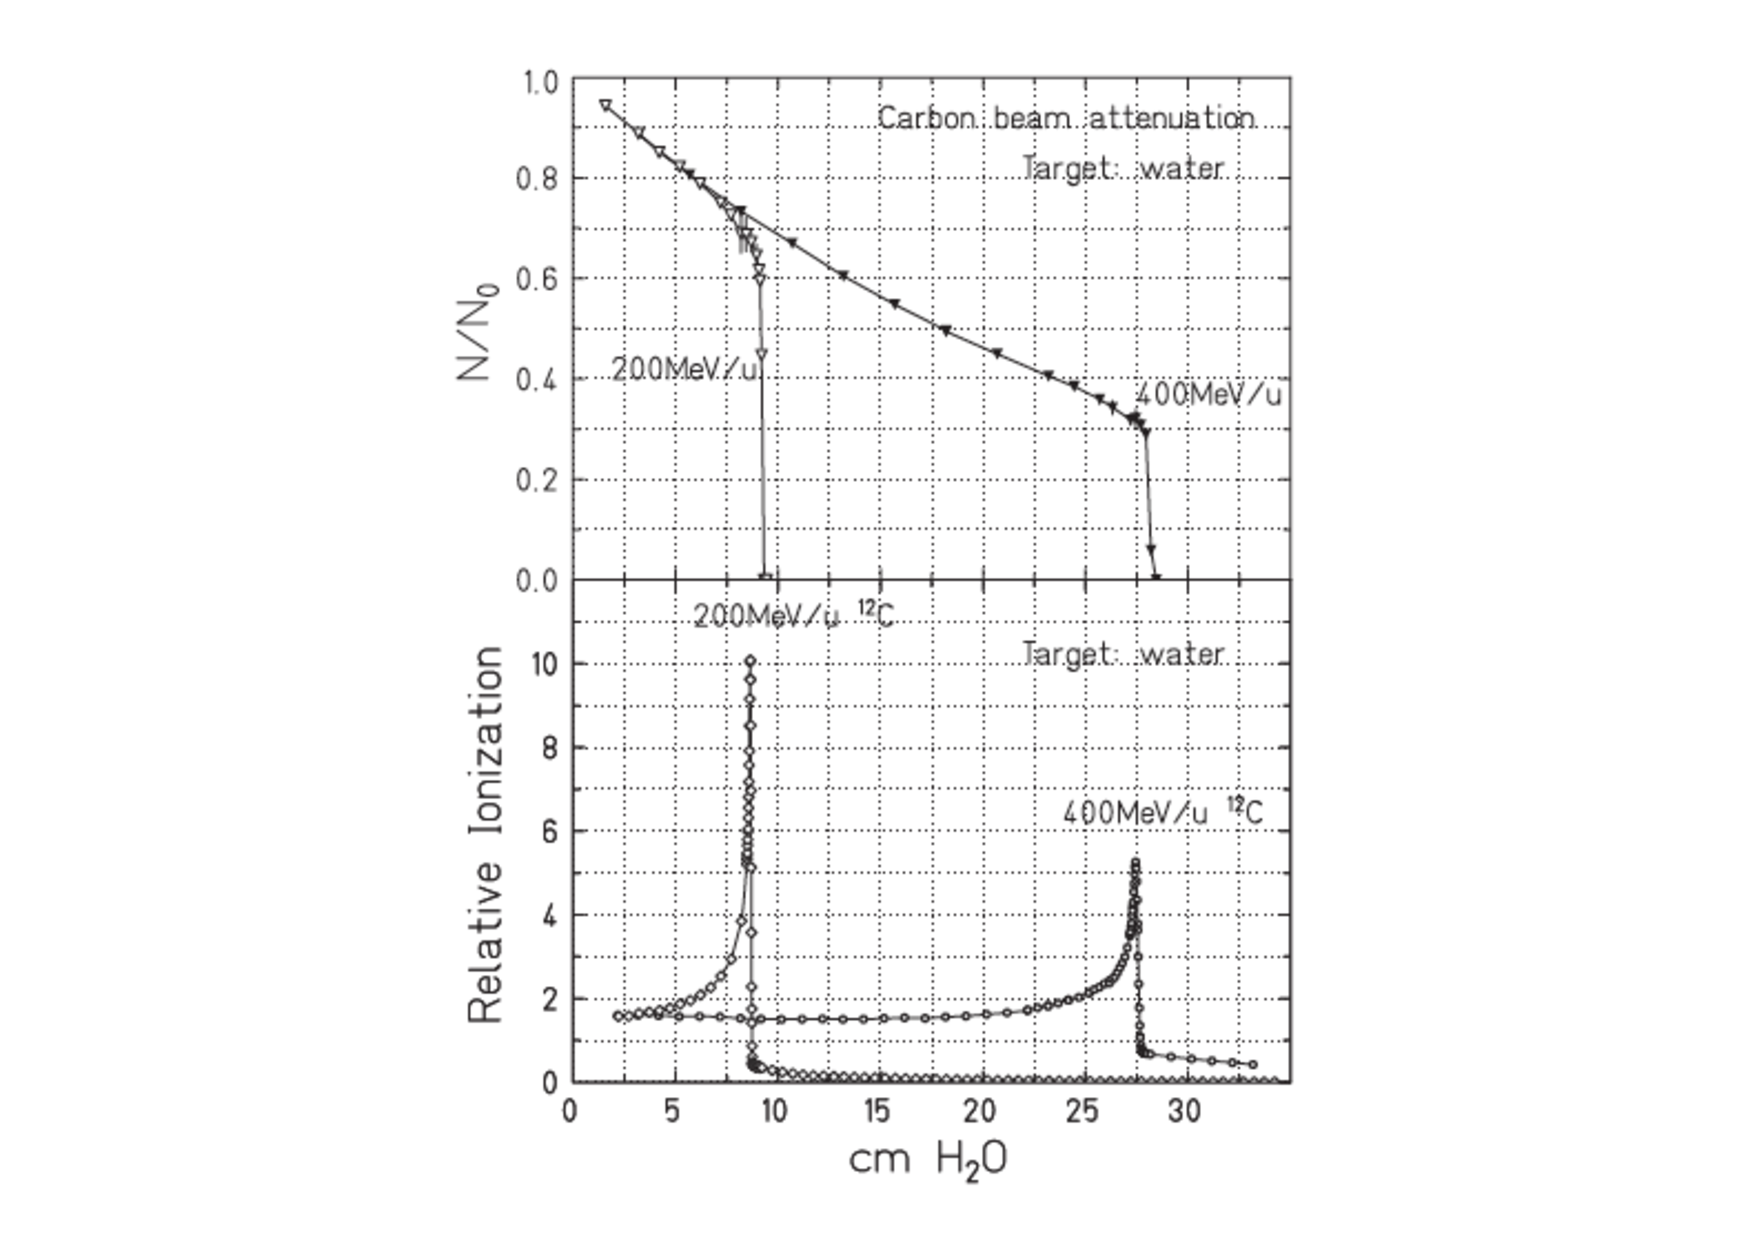
\includegraphics[width=1.2\linewidth, trim={1.5cm 0 1.5cm 0}, clip = true]{03_GraphicFiles/chapter1_Introduction/primaryLoss_Cion.pdf}
\caption{Primary particle fluence loss (top panel) and corresponding Bragg peaks (bottom panel) of carbon ion beams as a function of the depth in water for two initial beam energies. In~\cite{Haettner2006}.}
\label{chap1::fig::nuclearReacLoss_Cion}
\end{subfigure}
\begin{subfigure}[t]{.49\textwidth}
\hspace{-0.6cm} 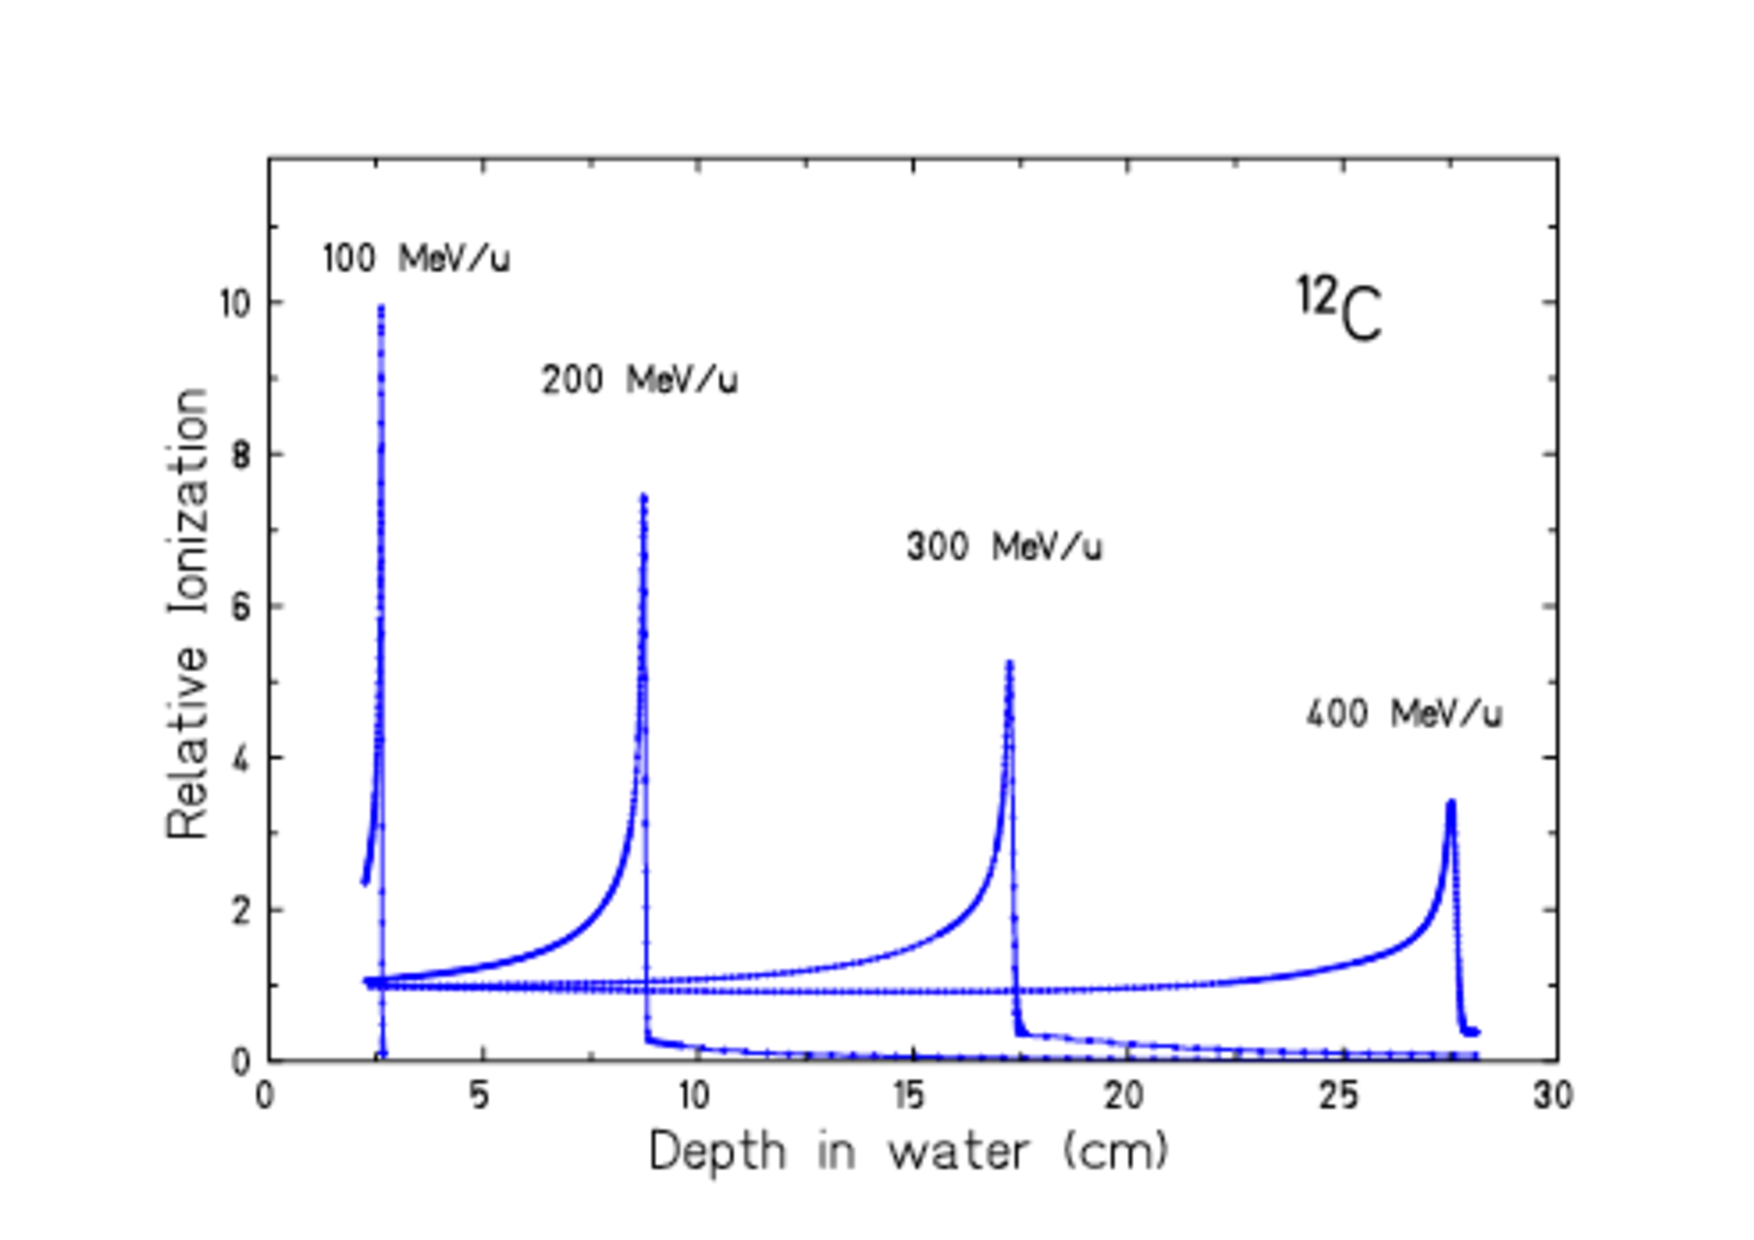
\includegraphics[width=1.1\linewidth, height = 5.9cm]{03_GraphicFiles/chapter1_Introduction/tailBragg.pdf}	
\caption{Integral dose as a function of the depth in water for proton beams at 7 different energies. The crosses represent experimental points, the solid lines are the results of dose model calculations. In~\cite{Pedroni2005}.}
\label{chap1::fig::TailBragg_p}
\end{subfigure}
\begin{subfigure}[t]{.49\textwidth}
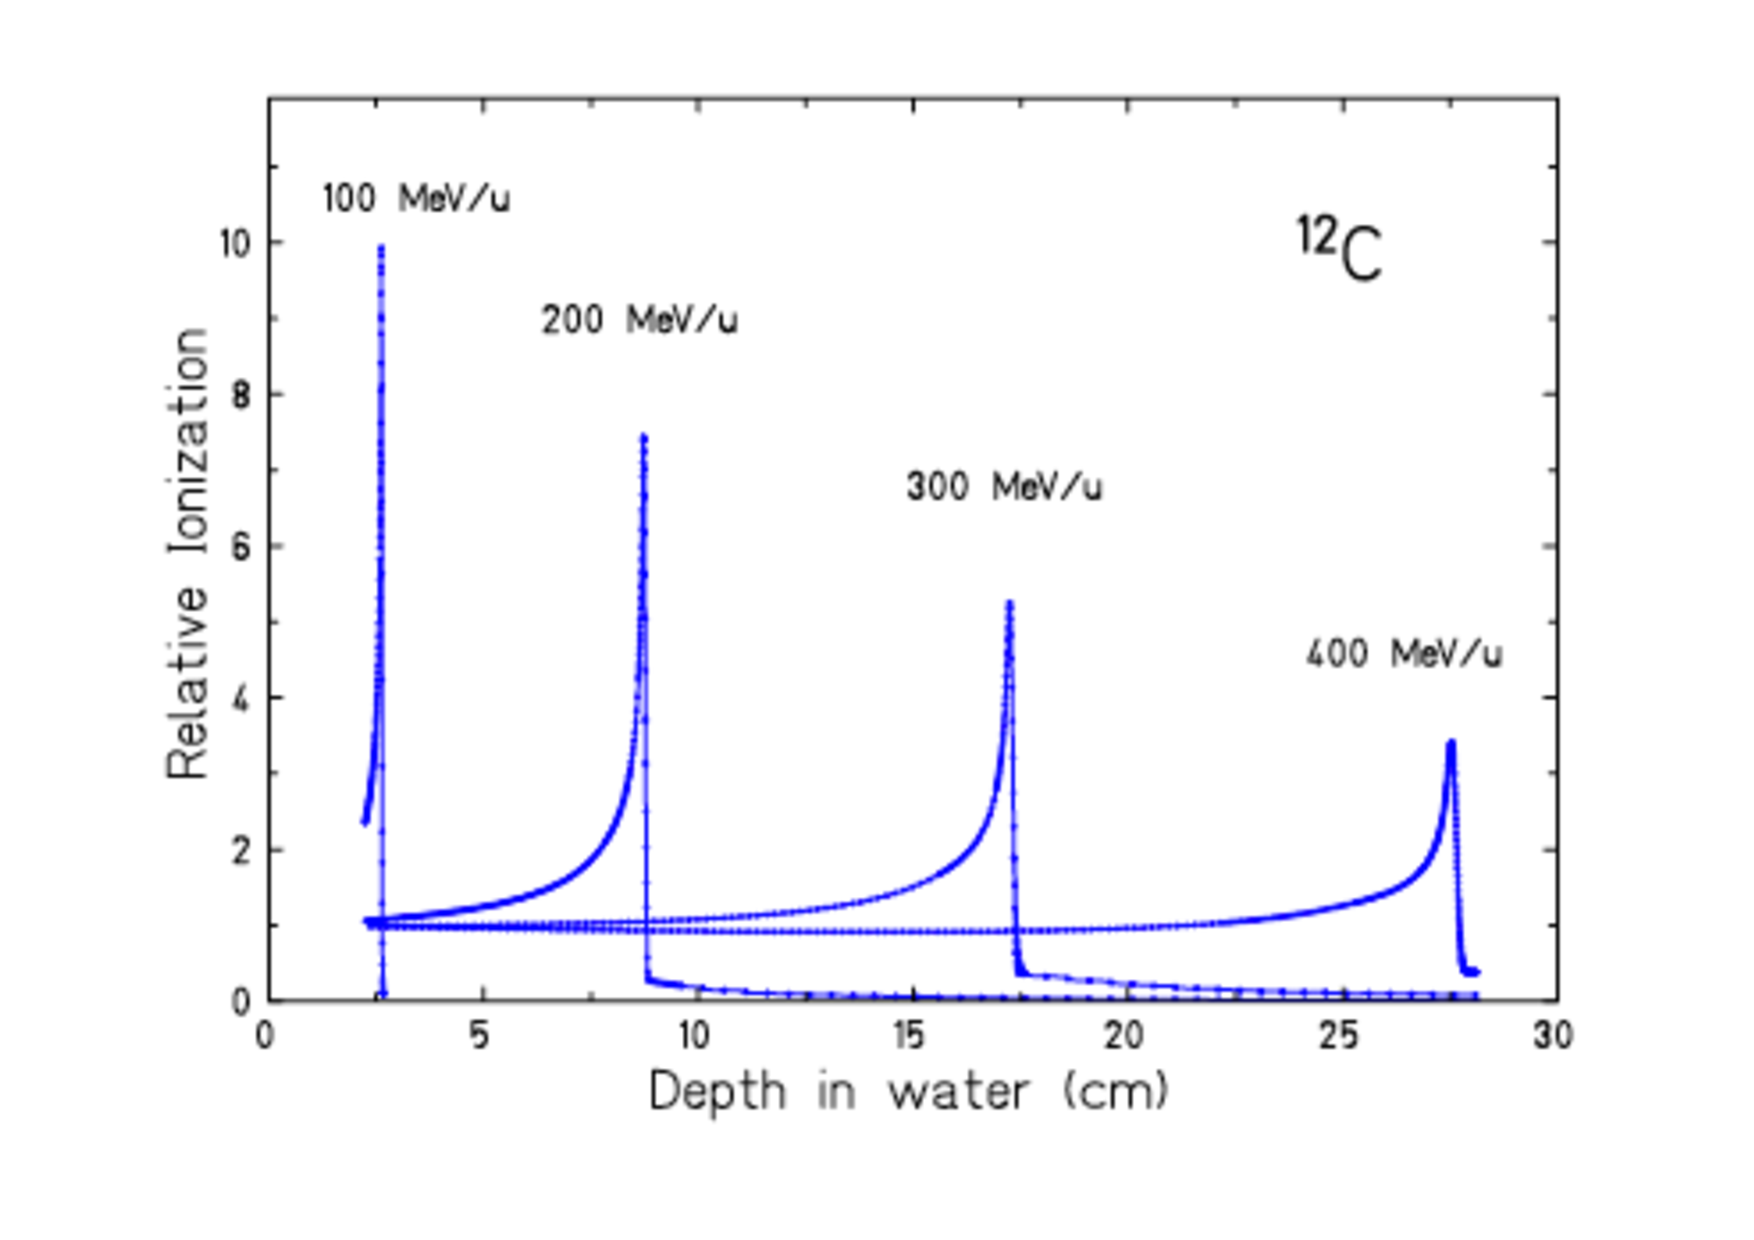
\includegraphics[width=1.2\linewidth, height = 6.05cm, trim = {1cm 0.4cm 0 0}, clip = true]{03_GraphicFiles/chapter1_Introduction/tailBragg_p.pdf}	
\caption{Measured relative ionizations for car\-bon ion beams stopping in water. In~\cite{Schardt2008}.}
\label{chap1::fig::TailBragg}
\end{subfigure}
\caption{Effects of nuclear interactions (first row) on proton (left column) and carbon ion (right column) beams and resulting dose distributions (bottom row).}
\label{chap1::fig::NuclearInt}
\end{figure}

Fragmentation processes have been deeply studied in nuclear physics and experimental data are available for many ion species at various energy~\parencite{Friedlander1982}. Dedicated studies for applications in radiotherapy started at Princeton~\parencite{MacCabee1974} with oxygen beams and were carried out for many years at the Bevalac in Berkeley~\parencite{Schimmerling1983, Schimmerling1989, Llacer1984, Llacer1990}, mainly with the neon beams used, at that time, for patient treatments. Analog studies were conducted later at the \gls{himac} facility~\parencite{Matsufuji2003, Matsufuji2005} and at \gls{gsi}~\parencite{Schall1996, Golovkov1997}, where several ion species have been compared. Results concerning the build-up characteristics of secondary fragments, also based on carbon ion irradiation of water targets, are published in~\cite{Haettner2006} and~\cite{Haettner2013}; in these works, 200 and 400~MeV/u ions have been used to investigate energy spectra and yields of the produced fragments at different angles and various depths along the beam path. A similar analysis has been carried out with 95~MeV/u carbon ion beam irradiation data collected at \gls{ganil}: in this case, \gls{pmma} thick targets (5, 10, 15, 20 and 25~mm) have been used~\parencite{Braunn2010, Braunn2011}. The obtained results have been compared to simulated data produced with fragmentation models implemented in Geant4 and mentioned in previous paragraphs, such as the \gls{bic} (based on the \gls{inc}) and the \gls{qmd} models, showing that model improvements were still needed to reproduce the experimental data.
Indeed, detailed information about fragmentation can be retrieved via Monte Carlo simulations and used to evaluate the impact on the delivered dose. As an example, in~\cite{Wroe2005} the authors studied in simulation the impact of nuclear reactions in the dose delivered with proton beams in different targets, like water, tissue equivalent plastic, and \gls{icrp} muscle, bone and adipose. Simulations published in~\parencite{Grassberger2011} of 160~MeV protons in water allowed to estimate the dose contributions given by primary particles (between 90\% and more than 99\% of the total depending on the range), with the remaining fraction of dose mainly connected to secondary protons and $\alpha$ particles: negligible dose is given by heavier fragments. A more intense dose contribution from heavier fragments is expected for carbon ion irradiation, but an accurate Monte Carlo simulation of these processes is still a challenge. The dose deposition in the distribution tail beyond the Bragg peak has been also studied in simulation: in~\cite{Francis2014}, for example, the dose connected to nuclear fragments has been estimated in 36\% of the total. 

As mentioned, in addition to charged fragments, nuclear interactions also produce gammas, mainly originating from atomic de-excitation processes (prompt-gammas) or from the annihilation of positrons emitted by $\beta^+$-emitter fragments ($^{10}$C, $^{11}$C, $^{13}$N, $^{14}$O, $^{15}$O), and neutrons, which can induce the emission of further gammas. All the secondary particles which can be absorbed by the target contribute to the total dispensed dose, while the others (with the exception of neutrons), escaping the target volume, can be exploited for non-invasive measurements of beam and target features. In particular, different techniques have been proposed and tested to measure secondary protons and gamma rays (both prompt-gammas and positron-annihilation gammas) with the aim of retrieving information about the ion range and obtain an online treatment verification. A detailed discussion about this topic will be given in section~\ref{chap1::subsec::uncertainty}.

Focusing on neutrons, which are produced in large quantities and over a wide energy range, they cannot be exploited for primary ion range monitoring since their detection is not correlated with the ion path in matter~\parencite{Testa2010}. The neutron signal can be used to retrieve dosimetric information in vivo, as reported in~\cite{Carnicer2014}: the research group at the \gls{cal} studied the secondary radiation in the proton ocular treatment room as a  function of the beam modulation, with a large volume ionization chamber. A strong correlation was found between the secondary ambient dose equivalent per proton dose and proton dose rate, which enables in vivo dosimetric verification independtly from the beam monitoring system. In any case, neutrons must be modeled with care in order to evaluate the safety measures to be implemented in treatment centers~\parencite{Newhauser2002}, as well as the implications in the delivered dose and secondary cancer probability~\parencite{Newhauser2011}. The dose contribution caused by secondary neutrons strongly depends on the beam delivery system (see section~\ref{chap1::subsec::beamDelivery} for the description of the beam delivery systems), as demonstrated in~\cite{Gottschalk2006}. In particular, passive elements used for beam shaping have been identified as one of the main sources of secondary neutrons contributing to the total delivered dose to the patient~\parencite{Yan2002}, so that in modern facilities deflecting elements are set after the passive modules in order to limit the neutron flux towards the target. It is interesting to notice that the amount of produced neutrons and resulting dose is comparable for protons and carbon ion irradiation, even if the neutron yield is higher for carbon ions: this is due to the different beam intensities used in clinics for the two species, with more than a factor 20 in favour of protons. In~\cite{Gunzert-Marx2008}, the total dose due to secondary neutrons has been estimated for 20 Gy absorbed dose during 200~MeV/u carbon ion irradiation of a water target, and it resulted in 1\% of the total absorbed dose. Finally, if compared to photon standard radiotherapy at high acceleration voltage (about 25~MV), the neutron dose associated to ion beam therapy treatments results to be smaller, as demonstrated in recent studies~\parencite{LaTessa2012, Schneider2015}. 

In the following section, the attention is focused on the biological aspects of this cancer treatment modality.


\subsection{Biological effects of ion beam therapy}\label{chap1::subsec::bioEffects} 
In addition to the already presented physical differences between photon radiation therapy and ion beam therapy treatments, a fundamental aspect to be addressed is the biological effect of such radiations. In the following, the main biological implications of radiation therapy are summarized with the aim of highlighting the favorable contribution given by charged particles with respect to photons and, at the same time, discuss some controversial points~\parencite{Paganetti2013}.

Any kind of radiation interacting and deposing energy in human tissues causes ionizations which lead to cellular and molecular effects. The effectiveness of ionizing radiation in curing cancer is based on the consequences produced by these ionizations, which can affect the double-helical DNA macro-molecules inducing various kinds of damages. In addition to this, other targets are also involved in the cell response to radiation, such as mitochondria and cellular membranes. In most of the cases, localized DNA damages, also called strand breaks, can be repaired with cellular reparation processes. In case DNA breaks are in close proximity they can originate the so-called \glspl{dsb}, both with direct ionizations of indirect process (such as $\delta$-electron energy deposition and the creation of reactive chemical species). \figurename~\ref{chap1::fig::DNAdamages} shows a schematic view of the different kinds of DNA damages induced by radiations, together with their effects in case of  successful or unsuccessful reparation mechanisms. \glspl{dsb} are generally harder to be repaired and lead to cellular dysfunction and loss of genetic material, resulting in cell death or in the loss of reproductive capacity. It appears clear from this simplified presentation that not only the total absorbed dose, but also the ionization event distribution plays a major role in the determination of the radiation effectiveness~\parencite{Belli1992}.        
The absorbed dose is defined in ~\cite{ICRU1980, ICRU1998} as 

\begin{equation}
\mathrm{D} = \frac{\mathrm{d}\overline{\epsilon}}{\mathrm{d}m}
\label{chap1::eq::AbsDoseDef}
\end{equation}

where $\mathrm{d}\overline{\epsilon}$ is the mean energy imparted by ionizing radiation to matter of mass $\mathrm{d}m$. To be precise, the imparted energy must also be defined: in the same ICRU reports we find that 

\begin{equation}
\epsilon = R_{\mathrm{in}} - R_{\mathrm{out}} + \sum{Q}
\label{chap1::eq::impEnergyDef}
\end{equation}

with $R_{\mathrm{in}}$ and $R_{\mathrm{out}}$ the sum of the energies of all ionizing particles entering or leaving the volume, respectively, $ \sum{Q}$ the sum of all changes of the rest mass energy of nuclei and elementary particles in any nuclear transformations occurred in the volume due to the ionizing radiation.
As mentioned, for the same absorbed dose, the ability of killing tumor cells is linked to the nature of the delivered radiations via the ionization event distribution. It is useful here to introduce the concept of \gls{let}\myMarginnote{Linear \\ Energy \\ Transfer}, defined as the amount of energy deposited by a particle per track unit, directly related to the number of ionization per unit distance. In general, photons, x-rays and $\gamma$-rays are referred to as low-\gls{let} radiation, while the larger stopping power of protons and ions make them a high-\gls{let} kind of radiation. For photon radiation, the distribution of the caused lesions is approximately random, while it is more closely related to the particle track for high-\gls{let} primaries~\parencite{Lobrich1996} causing a clustering effect in radiation damage which has been verified to be effective for cell killing~\parencite{Holley1996, Rydberg1996}. This is due to the nature of interactions of photons and ions in matter, already detailed in the previous section. 
Photons transfer energy to the cells by photo-electric or Compton interactions, with rather low cross-sections which determine a small number of ionization events and freed electrons per incident photon within the cell volume. Such freed electrons can further create secondary electrons along their path, but many photons are required to depose the prescribed dose, and the resulting ionization cluster distribution is almost homogeneous. The physical interactions of ions determine a completely different distribution of the deposited energy, localized along the ion path. The dose imparted in the radial direction is governed by a large amount of low energy electrons (Auger electrons) emitted in ion-atom interactions (also a limited amount of high-energy $\delta$ electrons are created), which are scattered by the medium atoms (electrons and nucleus) and cause secondary ionizations. The cross-section of these ionizations exhibits a maximum at about 100~eV, corresponding to a mean free path of a few nm. Given the DNA molecule size, this effect leads to a high probability of creating \glspl{dsb} or correlated single-strand breaks. %Thus, the lesion complexity increases with \gls{let}, and the strand breaks more concentrated in space are hardly repaired by the involved cells. 
Cell survival studies~\parencite{Tobias1982, Blakely1984} verified these theoretical considerations showing that heavy charged particles have an increased biological effectiveness compared to x-rays. These data are generally analyzed with a parameterization of the cell survival curve through a \gls{lq} model~\parencite{Hall2012}

\begin{equation}
S(D) = \mathrm{exp}(-\alpha D - \beta D^{2})
\label{chap1::eq::survivalPar}
\end{equation}
where S is the survival fraction, D is the absorbed dose and $\alpha$ and $\beta$ are parameters which are experimentally determined, or obtained via radio-biological models (see section~\ref{chap1::subsec::treatmentPlan}). The $\alpha/\beta$ ratio is linked to the radio-sensitivity of cells: the smaller it is, the larger the DNA repair capability will be. This is the rationale for fractionation in radiation therapy. Indeed, the total dose planned for the treatment of malignant cells is delivered in fractions along several days, because split doses have the advantage to spare normal tissues, with low $\alpha/\beta$ ratio, more than tumors, showing higher $\alpha/\beta$ ratio. 

\begin{figure}
\begin{subfigure}[t]{.4\textwidth}
\centering
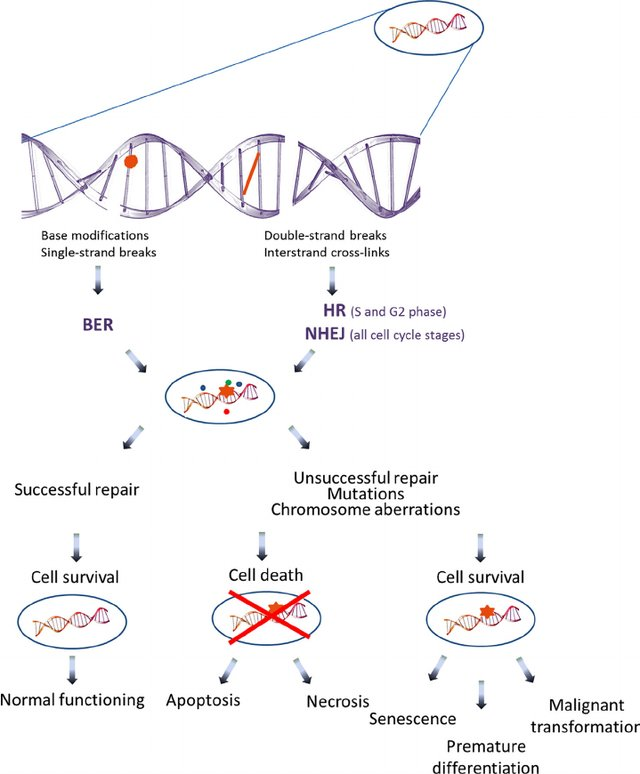
\includegraphics[width=0.99\linewidth]{03_GraphicFiles/chapter1_Introduction/DNAdamage.jpg}
\caption{Schematic representation of DNA damages caused by radiations. In~\cite{Arena2014}.}
\label{chap1::fig::DNAdamages}
\end{subfigure}
\begin{subfigure}[t]{.58\textwidth}
\centering
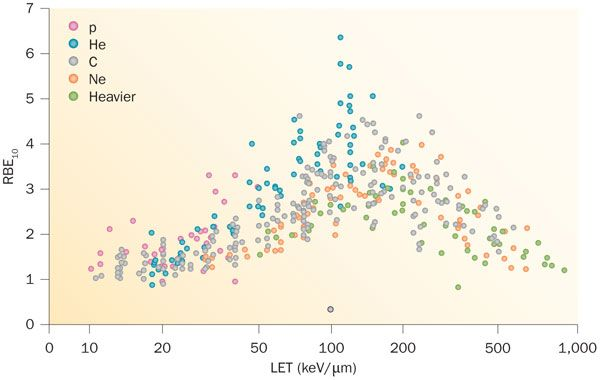
\includegraphics[width=0.99\linewidth]{03_GraphicFiles/chapter1_Introduction/rbeLET.jpg}	
\caption{\gls{rbe} dependence on \gls{let} for different particle species. \gls{rbe} is calculated at 10\% survival, \gls{let} values are given is keV/\charmum  ~in water. Different ions are represented in different colors. Data points are extracted from the \gls{pide} database. In~\cite{Durante2016}.}
\label{chap1::fig::rbelet}
\end{subfigure}
\caption{Ionizing radiations cause DNA damages in tissues, which are the basis for tumor radiation therapy. On the left side, the scheme presents the possible kind of damages induced by radiations on the cell DNA. The radiation effectiveness in killing cells is then related to the distribution of ionization events, which is all the more dense for high-\gls{let} primaries at low energies. The \gls{rbe} is then enhanced for this kind of radiation. On the right side, the \gls{rbe} is related to the \gls{let} for different ion species.}
\label{chap1::fig::NuclearInt}
\end{figure}
     
Given the complex scenario presented till here, it is clear that the physical absorbed dose is not sufficient to describe the effect of the delivered radiation treatment, and weighting factors based on radiation protection data have been introduced to account for both the biological properties of ions and the response of different tissues. \myMarginnote{Relative \\ Biological \\ Effectiveness}In order to transfer the experience from photon data to ion irradiation and to create a common evaluation parameter, the more powerful and versatile concept of \gls{rbe} has been introduced. The \gls{rbe} is defined as the ratio between the photon and ion doses necessary to produce the same biological effect (isoeffective dose):

\begin{equation}
\left. \mathrm{RBE} = \frac{D_{\mathrm{photon}}}{D_{\mathrm{ion}}}\right|_{iso}
\label{chap1::eq::rbeDef}
\end{equation}

where $D_{\mathrm{photon}}$ and $D_{\mathrm{ion}}$ are the absorbed dose for photon and ion irradiation. Notwithstanding the apparently simple definition, \gls{rbe} results to be a very complex quantity, but for the moment the only one really used in clinics. It depends on several physical and biological parameters, such as \gls{let}, dose, dose rate, fractionation scheme, particle type, target biological features (radiosensitivity, oxygen concentration, etc.)~\parencite{Durante2009}. As a result, the \gls{rbe} value changes along the primary ion path in matter, and is very difficult to be accurately predicted at the treatment planning stage. As an example, the dependence on \gls{let} is shown in \figurename~\ref{chap1::fig::rbelet}.  Although an accurate prediction is difficult to be obtained, the overall evolution of the \gls{rbe} as a function of \gls{let} demonstrate a further advantageous feature of ions with respect to photons. From very low \gls{let} to approximately 100-200~keV/\charmum ~, the \gls{rbe} increases: an overkilling effect determines then a drop at very high \gls{let} values. Thus, \gls{rbe} is higher for low energetic high-\gls{let} particles, which cause larger ionization density as their velocity decrease. This effect means that in the Bragg peak region the biological effectiveness of such radiations is more pronounced with respect to the plateau entrance area, where healthy tissues are spared. The \gls{rbe} enhancement for increasing \gls{let} is at present neglected in proton therapy, and a constant value of 1.1 is implemented in the clinical routine. This point is deeply discussed in the last years, and many simulation results and models have been produced to verify or propose modification to this usage~\parencite{Giantsoudi2013, Sethi2014, Guan2015, Jones2015, McNamara2015, Giovannini2016}. Anyway,  it is verified that a significant increase in \gls{rbe} with respect to photons can only be achieved with heavier ions, as also shown by the experimental data reported in \figurename~\ref{chap1::fig::rbelet}. For this reason, clinical trials have been conducted at the Lawrence Berkeley Laboratory starting from 1975 on different ion species such as He, Ne, N, O, C, Si, Ar~\parencite{Castro1995}. Very heavy ions have the advantage of providing very-high \gls{let} (and so \gls{rbe}) in the Bragg peak region, useful to overcome cell killing capability limitation due, for example, to cell oxygenation effects (discussed in the following)~\parencite{Blakely1984}. On the other side, heavy ions also show very high \gls{let} in the entrance region, which is not desirable. These results led to the implementation of carbon ion therapy, together with proton therapy, as a good comprise between radio-biological enhanced effectiveness in the target region (carbon-ion \gls{rbe} ranges between 3 and 4 in the Bragg peak - see~\cite{Wilkens2008}) and limited \gls{let} in the entrance plateau. 
As outlined in previous lines, a further parameters to account for in the evaluation of the biological effects of radiations is the cell oxygen status \myMarginnote{Oxygen Enhancement Ratio}. If compared to healthy tissues, tumor masses can grow in size producing malignant cells, and tumor core generally show lower oxygen levels. Even if the reason is not completely explained, hypoxic conditions cause an increased cell radio-resistance, probably linked to the reduction of indirect DNA damages induced by reactive chemical species. This effect is quantified via the \gls{oer}, 

\begin{equation}
\mathrm{OER} = \frac{D_{\mathrm{hypoxic}}}{D_{\mathrm{aerobic}}}
\label{chap1::eq::oer}
\end{equation}

with $D_{\mathrm{hypoxic}}$ and $D_{\mathrm{aerobic}}$ the absorbed dose for normal and reduced oxygen level resulting in the same clinical effect. Its value is about 3 for conventional radiation~\parencite{Schardt2010}, while it is reduced for ion irradiation due to the increased \gls{rbe}, making them fundamental for curing tumors with hypoxic regions.

Only some of the biological aspects have been cited here, and all their clinical implications should be ideally taken into account for an accurate treatment planning. This is the reason why some of the points discussed here will be further addressed in section~\ref{chap1::subsec::treatmentPlan}. 

\subsection{Accelerators and beam delivery}\label{chap1::subsec::beamDelivery}

The goal of ion beam therapy is to treat deep-seated tumors with a conform dose distribution. Different ion species, hadrons and charged particles in general have been and are under study for the clinical application (neutrons, charged pions, antiprotons, helium ions - i.e. alpha particles -, heavier ions like lithium, oxygen, up to silicon ions), but only two are at present implemented for the patient treatments: protons and fully stripped carbon ions~\parencite{Degiovanni2015}. The ability of treating any kind of tumor at any depth in human body relies on the possibility of providing the employed particles enough energy to obtain a range of about 25~cm in soft tissues. The ions employed in treatment must be then accelerated to about 60-70\% of the speed of light ($\beta$ = 0.6-0.7, see~\cite{Durante2016}) via different acceleration techniques and machines. This translates into maximum energy values of the order of 200-250~MeV and 4500~MeV (i.e. 375~MeV/u) for protons and carbon ions, respectively~\parencite{Braccini2010}. In order to achieve the desired ion energy,  sizable accelerators are needed and different solutions have been explored; at present, cyclotrons and synchrotrons  are clinically implemented and available on the market. In the following, after a brief historical introduction, we sketch the main characteristics of the accelerators used in clinics, and we highlight the main features which are reflected in the treatment delivery. In addition to this, the beam delivery systems are described. Moreover, an overview of the main directions followed for the future acceleration and beam delivery techniques upgrade is provided. 

\subsubsection{Accelerators for ion beam therapy}\label{chap1::subsubsec::accelerators}
The way towards the possible application of ion beams in therapy \myMarginnote{Cyclotrons} (proposed only later by Wilson - see~\cite{Wilson1946}) was opened by the invention of the cyclotron by Ernest Orlando Lawrence in 1929~\parencite{Lawrence1932}, which added a magnetic field to the recently proposed linear accelerator~\parencite{Wideroe1928}. A cyclotron is composed of two hollow electrodes with a frequency-alternating voltage applied between them, which accelerates the charged particles at each revolution. The circular trajectory is obtained thanks to a fixed vertical magnetic field. A scheme of the main components of a cyclotron is sketched in \figurename~\ref{chap1::fig::cyclotron}.

\begin{figure}[!htbp]
\centering
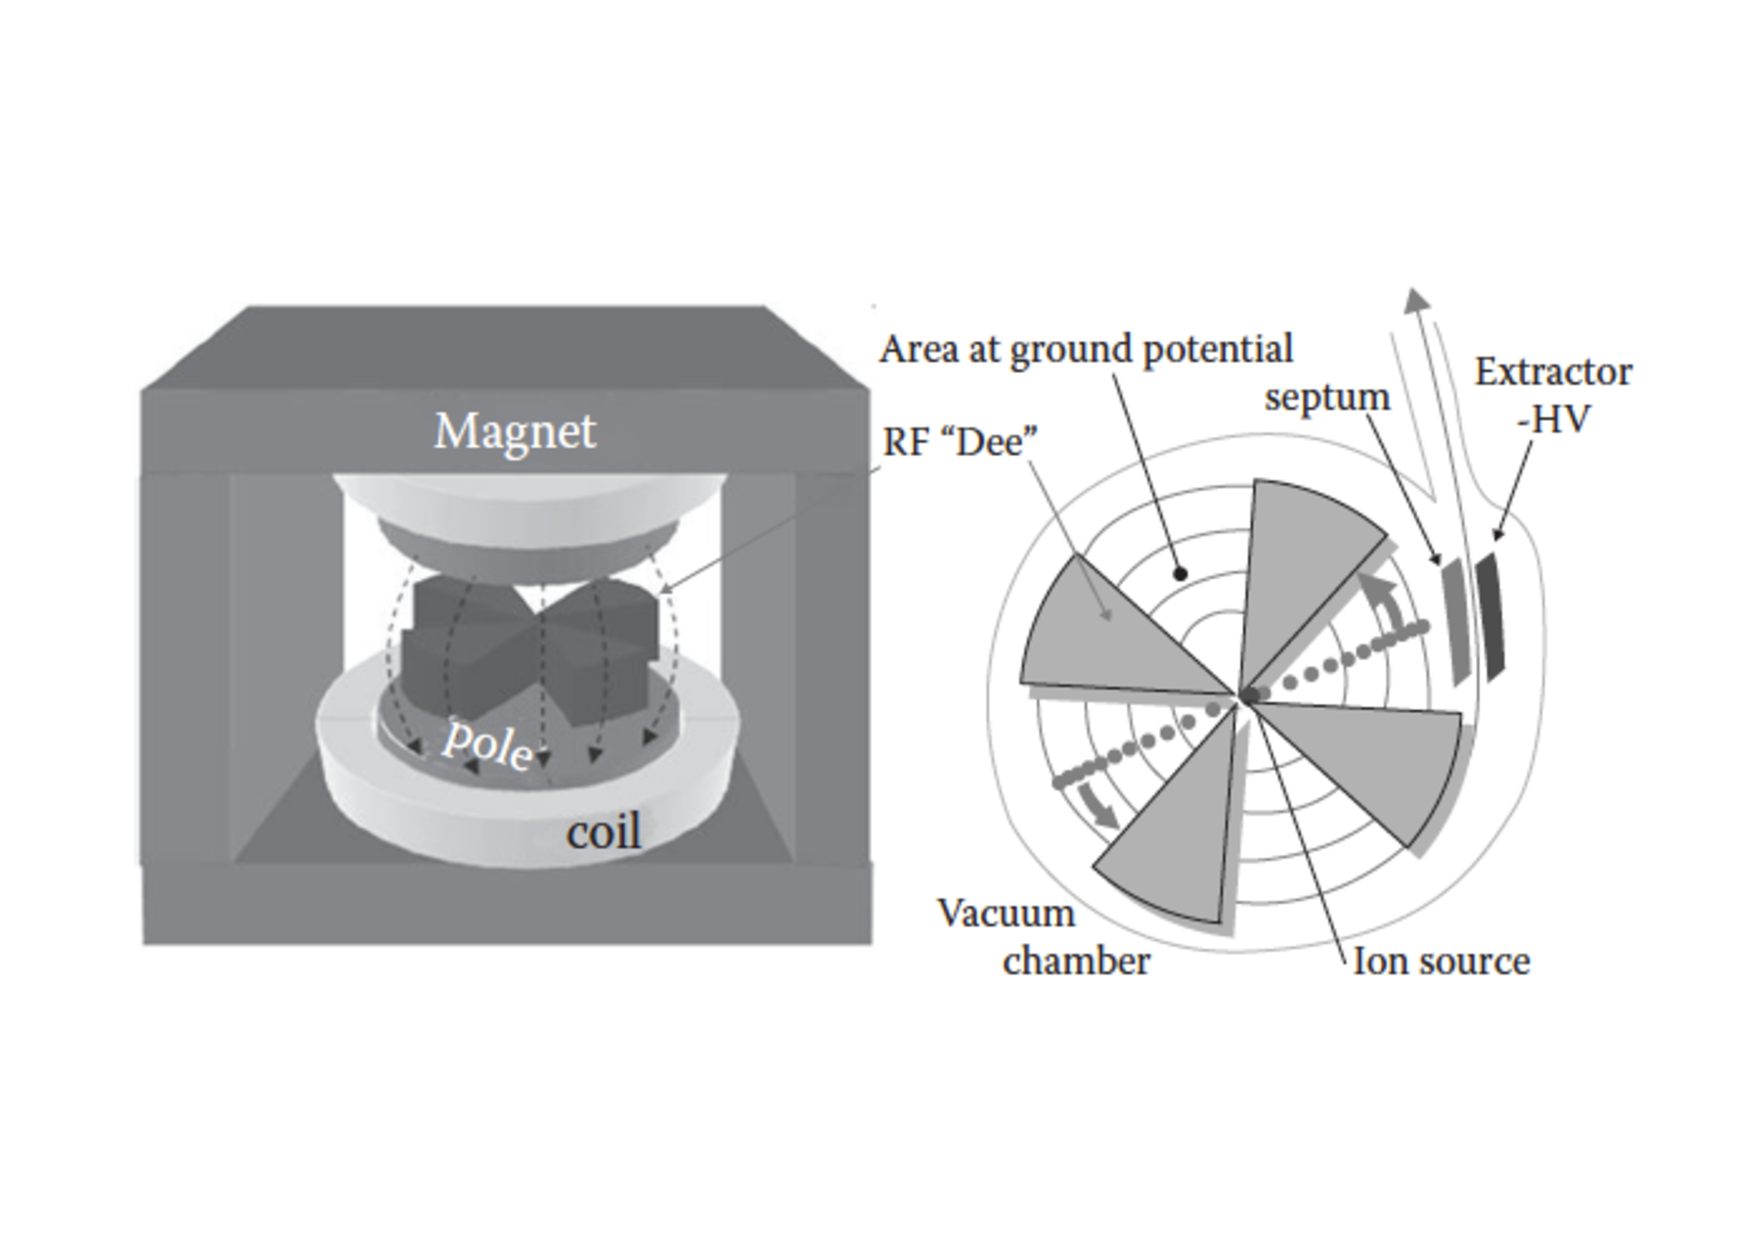
\includegraphics[width=0.7\textwidth]{03_GraphicFiles/chapter1_Introduction/cyclotron.pdf}
\caption{Schematic view of the main components of a cyclotron accelerator. On the left side the magnet is sketched together with the radio-frequency elements (\enquote{Dees}), which are also shown on the section depicted on the right side, with the ion source in the center. In~\cite{PaganettiBook2012}.}
\label{chap1::fig::cyclotron}
\end{figure} 

Nuclear physics saw a paramount development thanks to this invention, but also in the medical field the impact was remarkable. Already in 1935, Lawrence produced the first cyclotron-originated radionuclides, then used for radiotracing, diagnosis and treatment. The first cyclotron-based treatment was performed with fast neutrons (i.e. with kinetic energies between a few MeV and a few tens of MeV) in 1938, following a paper by Gordon Locher who underlined the therapeutic potentialities of neutrons~\parencite{Locher1936}; the neutrons were produced by bombarding a beryllium target with cyclotron-accelerated deuterons~\parencite{Stone1940}. The unfavorable depth-dose distribution of neutrons and the difficulties linked to their collimation finally led to abandon the neutron treatments in 1948~\parencite{Stone1948} and move towards proton-beam treatments in the 50's: neutrons were revised in 1965 by Catterall in London~\parencite{Catterall1971} and are still used today in \gls{bnct} techniques~\parencite{Barth2005, Nedunchezhian2016}. As already mentioned in section~\ref{chap1::sec::ionBeamTher}, the first proton therapy treatment was conducted by Cornelius Tobias,  and John Lawrence with the Lawrence cyclotron in 1954~\parencite{Tobias1955, Tobias1958}. Between 1954 and 1974, more than 100 patients were treated in Berkeley with cyclotron-accelerated protons. In parallel, in 1957 the first tumor was irradiated with protons at the Uppsala cyclotron in Sweden~\parencite{Larsson1962}, and an intensive proton therapy program, leaded by Robert Wilson, was started in Harvard with a new-built cyclotron~\parencite{Wilson2004}. Following these first experiences, new physics laboratories decided to set up proton beams for therapy (USSR, Japan, Switzerland), until the creation of the first hospital-based center, built at the Clatterbridge Oncology Center in the United Kingdom, which started operating in 1989 with a 62.5~MeV cyclotron. This historical overview shows how the cyclotron technology has soon spread all over the world, not only in research centers, but also for therapy purpose. The present cyclotron machines, which are now commercially available by different providers,  still rely on the same accelerating principle as the first Lawrence system, but the technology has greatly advanced.  In particular, the vertical magnetic fields in charge of bending the particles on a spiral trajectory has been improved, giving the beam the desired transverse compactness. Moreover, the beam extraction efficiency has been improved, and multiple extractions are now possible to supply different transport lines.
Moreover, synchrocyclotrons are a solution compatible with hadrontherapy applications. Based on the cyclotron accelerating principle, a synchrocyclotron presents a variable frequency for the alternating voltage which is used to compensate for relativistic effects when the accelerated ions approach the speed of light. Such a solution has the advantage of allowing for the creation of more compact systems with high magnetic fields, and is at present exploited for commercial accelerators by the main providers.  
In addition to cyclotrons and synchrocyclotrons, other accelerating machines \myMarginnote{Synchrotrons} initially developed for fundamental research have been translated to medical applications and are nowadays knowing a large diffusion: the synchrotrons. While the cyclotron present a fixed-value magnetic field, so that the radius of the beam trajectory increases during the acceleration process, in the synchrotron the trajectory radius is kept constant thanks to the variation of the bending magnetic field. The boost is provided by radio-frequency cavities, based on the same principle as the one composing linear accelerators: the radio-frequency increases to follow the particle revolution speed, and this acceleration principle allows to overcome the cyclotron energy limitation, as well as to obtain beam at different energies by tuning the extraction process. The invention is based on the independent ideas of Vladimir Veksler~\parencite{Veksler1944} and Edwin McMillan~\parencite{McMillan1945}: the latter both coined the name of the machine in its letter, and constructed the first electron synchrotron in 1945 in Berkeley. Some years later, the first proton synchrotron was designed in 1952 by Sir Marcus Oliphant, who already published a preliminary sketch of the machine in 1943~\parencite{Oliphant1943}. As for the cyclotron case, several years have been required to see the construction of the first hospital-based hadrontherapy facility using a synchrotron. The first center was built at Loma Linda University in California, were a 7-m-diameter synchrotron constructed by Fermilab was installed and started treating patients in 1990. The center has been a pioneer in the field also for the presence of three 10-m-diameter rotating gantries.  
After the clinical studies performed at the University of Tsukuba, in Japan, between 1983 and 2000, with the treatment of about 700 patients with synchrotron proton beams, a second hospital-based center was built and equipped with an Hitachi synchrotron and two rotating gantries. 
Since the first use of synchrotrons for treatment purpose, several improvements have been achieved in the accelerator technology to better adapt its features to the hadrontherapy needs. In particular, the beam size can be now reduced with strong focusing optics, and the beam energy can be varied on a single spill basis (1-2~s). 
At present, all the hadrontherapy facilities in operation are based on circular accelerators (cyclotrons and synchrotrons): proton beams are produced with both the solutions, while only synchrotron-produced carbon-ion beams are used. In \figurename~\ref{chap1::fig::acceleratorSize} the size of different accelerators design is compared (CABOTO is still at the design stage, the \gls{iba} / ARCHADE superconducting carbon cyclotron in France is under design, while \gls{hit}, \gls{cnao} and the SIEMENS accelerator are at present in operation).

\begin{figure}[!htbp]
\centering
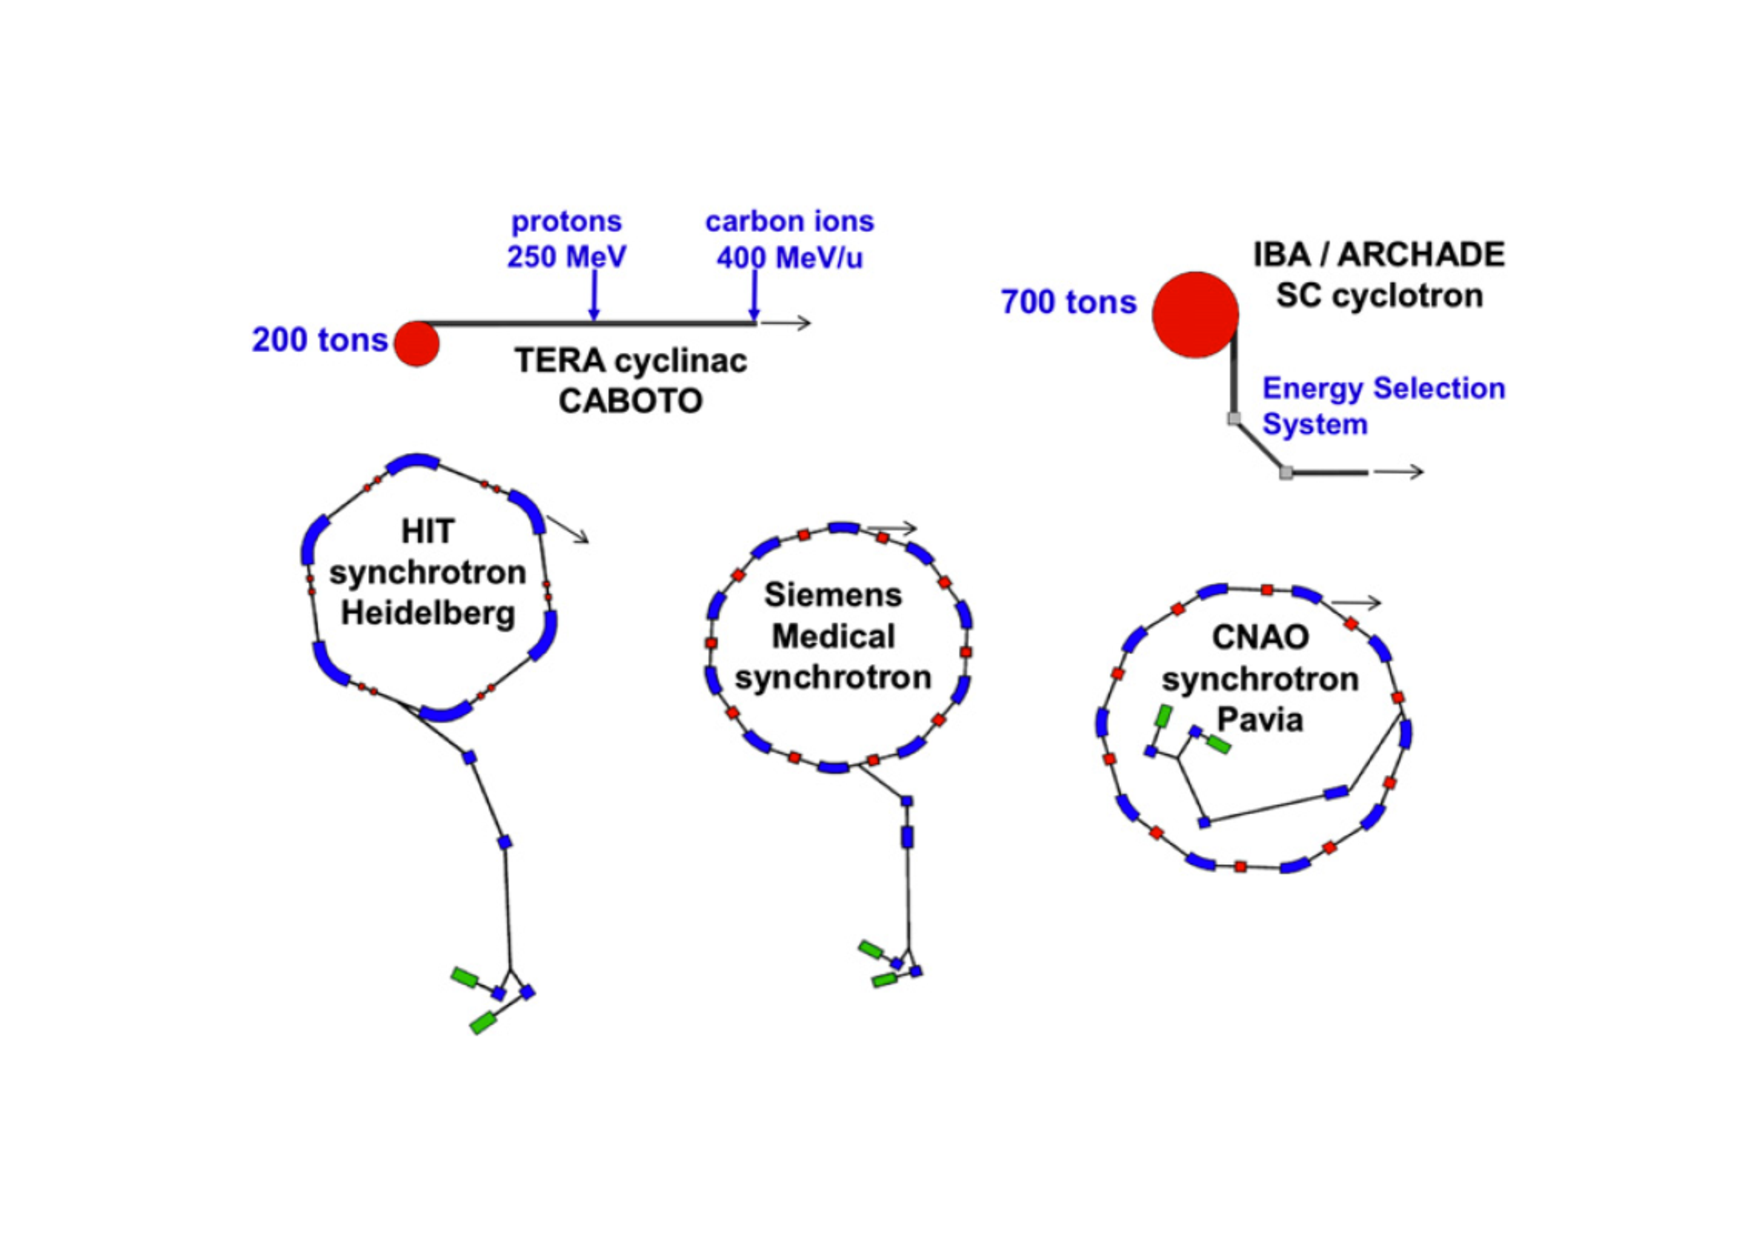
\includegraphics[width=0.7\textwidth]{03_GraphicFiles/chapter1_Introduction/acceleratorSize.pdf}
\caption{Comparison of the size of various ion accelerators for hadrontherapy. CABOTO is a cyclinac studied by the TERA Foundation; the superconducting cyclotron, designed by \gls{iba}, will be installed in Caen, France, within the ARCHADE project; \gls{hit} and \gls{cnao} are in operation in Heidelberg, Germany and Pavia, Italy, respectively; the SIEMENS synchrotron is installed in Marburg and Shangai. In~\cite{Amaldi2010}.}
\label{chap1::fig::acceleratorSize}
\end{figure} 

In the last years, novel approaches have been proposed \myMarginnote{Novel acceleration approaches} to improve the present accelerators and beam features, mainly for what concerns the beam quality and the machine size and cost. It is worth to mention the \gls{ffag} accelerator, which combines the fixed magnetic field and variable radio-frequency with separated sector magnets~\parencite{Sheehy2016}. This approach allows for the production of higher intensity beams with respect to synchrocyclotrons, and for the variation of the extracted beam energy at high repetition rate. Some designs have been proposed for hadrontherapy applications in the last decade~\parencite{Antoine2009, Peach2010}, but the present machine size still limits its spread in treatment centers. 
Furthermore, linear acceleration approach has been proposed since 1991 in both \enquote{all-linac}~\parencite{Lennox1991, Hamm1991} and \enquote{cyclinac}~\parencite{Amaldi2009b} solutions. In addition to the compactness, the main advantage of linacs is the possibility to continuously vary the output beam energy on a pulse to pulse basis; moreover, there is neither the need for complex injection or extraction systems, such the ones used in synchrotrons, nor the need of an energy passive modulation technique as the one used in cyclotrons (see section~\ref{chap1::subsubsec::BeamDel}). An extended description of linear accelerators for hadrontherapy is given in~\cite{Amaldi2009a}. Following the first successful prototypes tested by the TERA Foundation and the Italian \gls{infn} in the last twenty years~\parencite{Amaldi2004, Ronsivalle2011}, the \gls{cern} spin-off company \gls{adam} is proposing a commercial solution called \gls{light}. A further solution can be given by the \gls{dwa}~\parencite{Caporaso2009}, where the acceleration tube is made of High Gradient Insulator disks alternated with conducting elements. A laser pulse is used to activate the switching units connected to these conducting modules. Very interesting thanks to a reduced size, this acceleration scheme still suffers beam focusing issues; moreover, it presents very short pulses which force a very precise selection of the number of ion per pulses at the source level. Finally, the electric field needed for reducing the machine size till 2-2.5~m is of the order of 100~MV/m; this challenging value has not been achieved yet, even if a prototype is under study at the \gls{llnl}, with promising results~\parencite{Hettler2013, Zografos2013}. Another attractive technique is the so-called \enquote{laser driven} acceleration, based on the use of short and powerful laser pulses irradiating a thin target, with the generation of a plasma field~\parencite{Tajima2009}. The electrons emerging from this plasma are able to induce a strong electric field which accelerates the protons (or ions). Again, this solution would allow for the creation of very compact systems, with relatively simple and light beam optics, but some issues are still under study to be solved; in particular, the accelerated beam has an almost continuous energy spectrum which forces to implement energy selection solutions to be adapted to treatment purposes. 

\subsubsection{Beam time structure}\label{chap1::subsubsection::beamTimeStruct}

A particle beam can be described by a set of quantifying parameters which relates to single particle properties or to a collection of particles. In addition to the beam energy (which should be defined as an energy spectrum), beam current (which describes the beam intensity as the flux of particles per time unit) and emittance (transverse size and momentum), it is worth to describe in details what is defined as time structure. A basic distinction is made between continuous beams and bunched beams. Whenever particles are accelerated by means of radio-frequency varying fields, the accelerating machine output is a bunched beam, composed of bunches with fixed time length. Concerning the acceleration systems employed to produce clinical beams, synchrotron and cyclotrons (or synchro-cyclotrons) present strongly different time structures. In order to give an overall description of the typical time features of synchrotron- and cyclotron-produced beams, it is possible to distinguish between micro- and macro-structure. The macro-structure describes cycles of beam acceleration and extraction, the latter characterized by an internal micro-structure. By comparing the two cited kinds of accelerators, it is possible to approximate the cyclotron-produced beams as continuous, with a macro-structure characterized by sub-millisecond periods (depending on the specific machine) and approximately 10\% duty cycle (fraction of period with active ion delivery). Synchrotrons produce pulses which are separated in periods of several seconds, with duty cycles similar to the ones of cyclotrons (10$^{-1}$ on average). For synchro-cyclotrons, the duty cycle is approximately 10$^{-3}$. Each accelerator pulse (for both cyclotrons and synchrotrons), corresponding to one extraction cycle, contains several micro-bunches, creating the micro-structure. For cyclotrons, micro-bunches duration is in the ns scale, while a synchrotron micro-bunch can last several tens of ns. The period separating micro-bunches varies in the range of tens of ns for cyclotrons till hundreds of ns for synchrotron beams. 

Table~\ref{chap1::tab::beamTime} shows the orders of magnitude for the beam time structure for some particle accelerators used in the clinical routine. The differences between synchrotrons, cyclotrons and synchro-cyclotrons are evident. In addition, the beam typical intensity is reported.

\begin{table}[!htbp]
\centering
\caption{Orders of magnitude of main time structure parameters for some accelerators used in clinics. Reproduce from~\cite{Krimmer2017}.}
\label{chap1::tab::beamTime}
\begin{tabular}{P{2cm} P{2cm}  P{1cm} | P{1cm} P{2cm} P{2cm} P{2cm}}
\toprule
\rowcolor{myColorMainA!20} 
 	& &  \multicolumn{2}{c}{\textbf{Synchrotron} }& \textbf{Cyclotron C230 \gls{iba}} & \textbf{Cyclotron Varian} & \textbf{Synchro-cyclotron S2C2 \gls{iba}}\\
& & \underline{$^{12}$C} & \multicolumn{4}{c}{\underline{Protons}} \\
\midrule
\multicolumn{2}{l}{\textbf{Typical intensity (ions/s)}} & 10$^7$ & 10$^9$ & 10$^{10}$ & 10$^8$ - 10$^{10}$& $\sim$10$^{10}$ \\
\midrule
\textbf{Macrostruct.} & Period (s) & \multicolumn{2}{c}{1-10} & \multicolumn{2}{c}{/} & 10$^{-3}$ \\
								&  Duty cycle  & \multicolumn{2}{c}{10$^{-1}$} & \multicolumn{2}{c}{10$^{-1}$} & 10$^{-3}$ \\
\midrule
 & Bunch width & \multicolumn{2}{c}{20-50} & 1-2 & 0.5 & 8 \\
\textbf{Microstruct.}  &  Period (ns) & \multicolumn{2}{c}{100-200} & 10 & 14 & 16\\
 & Ions/bunch & 2-5 & 200-500 & 200 & 2-200 & 4000 \\
\bottomrule
\end{tabular}
\end{table}      

An accurate knowledge of the beam time structure is of utmost importance for the optimization of the interface to the beam delivery systems (see section~\ref{chap1::subsubsec::BeamDel}), for the treatment planning, as well as for treatment monitoring purpose. The design of detectors able to exploit the emission of secondary particles to retrieve beam range and dose information must account for the beam time structure in order to evaluate the best solution to deal with signal background, counting rate and read-out channel occupancy. This topic will be further discussed in section~\ref{chap1::subsec::uncertainty} where the sources of uncertainties affecting ion beam therapy treatment are described and the detection monitoring solutions are presented. In particular, for the specific case of \gls{pg} detection (one of the main topic of this thesis work), a complete overview is given in chapter~\ref{chap::2}. 

\subsubsection{Beam delivery systems}\label{chap1::subsubsec::BeamDel}

Once accelerated, the high-energetic ions must be delivered to the patient in order to be conform to the treatment specification, focusing the provided dose on the \gls{ptv}. As described and detailed in section~\ref{chap1::subsec::Physics}, the beam range can be varied by modulating the primary particle energy with the aim of covering the whole tumor volume. The Bragg curve obtained with a monoenergetic beam is called \enquote{pristine Bragg curve}, and can be used to irradiate a section of the target volume at a given depth. The superposition of several pristine Bragg curve is necessary to deliver the prescribed dose to the tumor, which has been previously modeled in three dimensions. In particular, the beam energy spectrum has to be spread in order to increase the axial dimension of the peak region, in the so-called \gls{sobp}. At the same time, the beam fluence must be adapted to avoid over-irradiation of the entrance region. An example of \gls{sobp} is given in \figurename~\ref{chap1::fig::pristine_sobp}. Note that the distal spot has a significantly higher fluence than proximal ones, since there is no contribution of higher energy particles. This is true for single field treatments , while for several field treatments different spot fluence structures can be used. This will have an influence on the sensitivity of the method used to control the position of the distal part of the \gls{sobp}, as discussed in section~\ref{chap1::subsec::uncertainty}. 

\begin{figure}[!htbp]
\centering
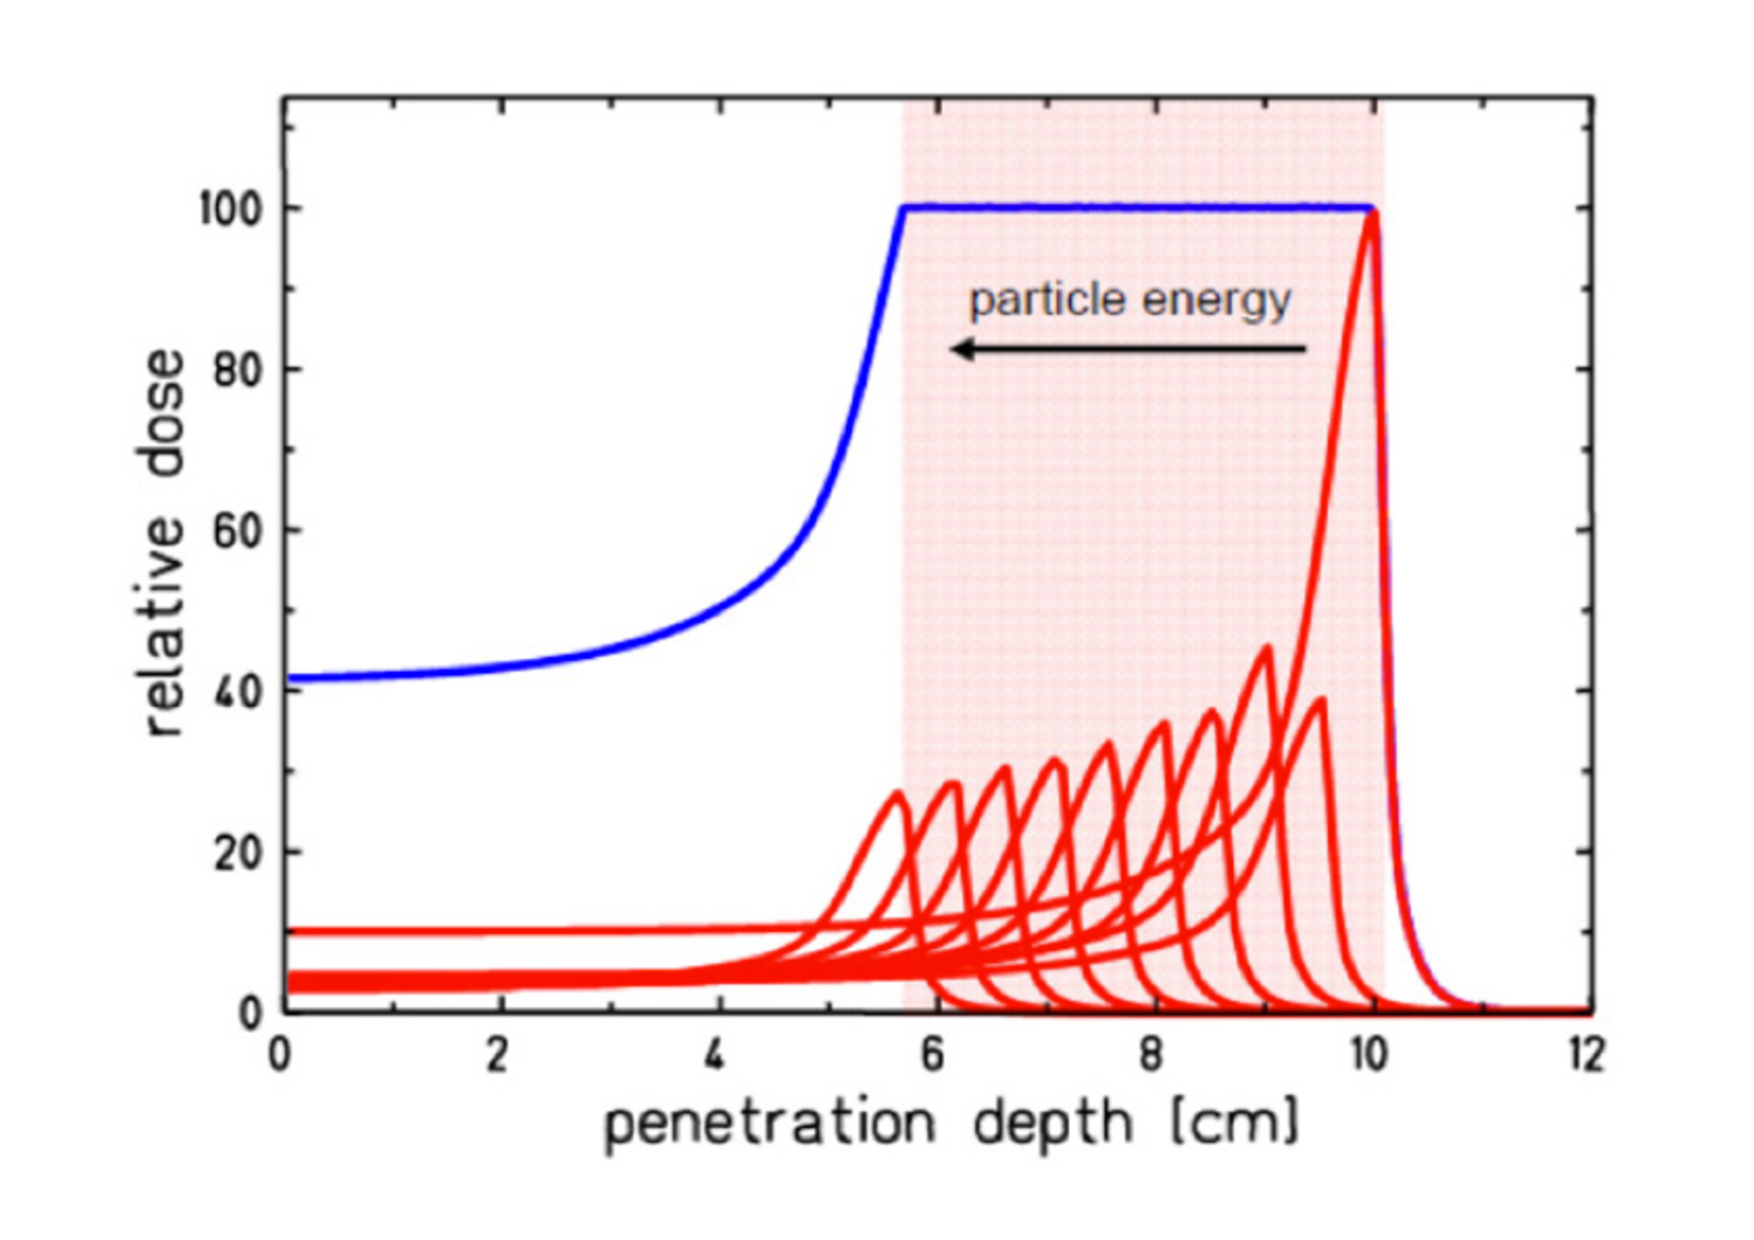
\includegraphics[width=0.7\textwidth]{03_GraphicFiles/chapter1_Introduction/pristine_sobp.pdf}
\caption{Example of \gls{sobp}. The target region is highlighted and the discrete pristine peaks composing the \gls{sobp} are sketched in red. In~\cite{Durante2016}.}
\label{chap1::fig::pristine_sobp}
\end{figure} 

All the described tasks are in charge of the beam delivery system, which must be optimized to interface with the accelerator and to the patient by transporting the beam to the treatment area and adjusting its features to obtain the desired dose distribution. 
The delivery systems implemented in clinics are based on two main strategies: passive beam modulation and active scanning. For an extensive presentation of this topic, refer to~\cite{Gottschalk2008}. The technique must be chosen according to the accelerator machine: it is important to remind that cyclotrons provide fixed energy beams with pulses separated by tens of nanoseconds, while in a conventional synchrotron the energy can be varied cycle by cycle, with short pulses generally separated by 1-2~s dead-time (see section~\ref{chap1::subsubsection::beamTimeStruct}). 

The passive beam delivery approach \myMarginnote{Passive beam shaping} generally applies to cyclotron-produced beams, and its principle is sketched in \figurename\ref{chap1::fig::passiveDelivery}. The beam extracted from the accelerator is fixed in size and energy, and is first broadened by scattering devices. Afterwards, a range modulator (generally a rotating wheel) is used to spread out the mono-energetic Bragg peak with the aim of covering the whole target thickness. The wheel periodically inserts material of varying thickness into the beam line, resulting in a range modulation with the desired features. The obtained \gls{sobp} can be shifted as a whole thanks to the addition of range shifters of fixed thickness. After the energy (range) adaptation, the beam is shaped according to the \gls{ptv} definition with collimators (often multi-leaf) and compensators, which are specific to each patient and irradiation port.  

\begin{figure}[!htbp]
\centering
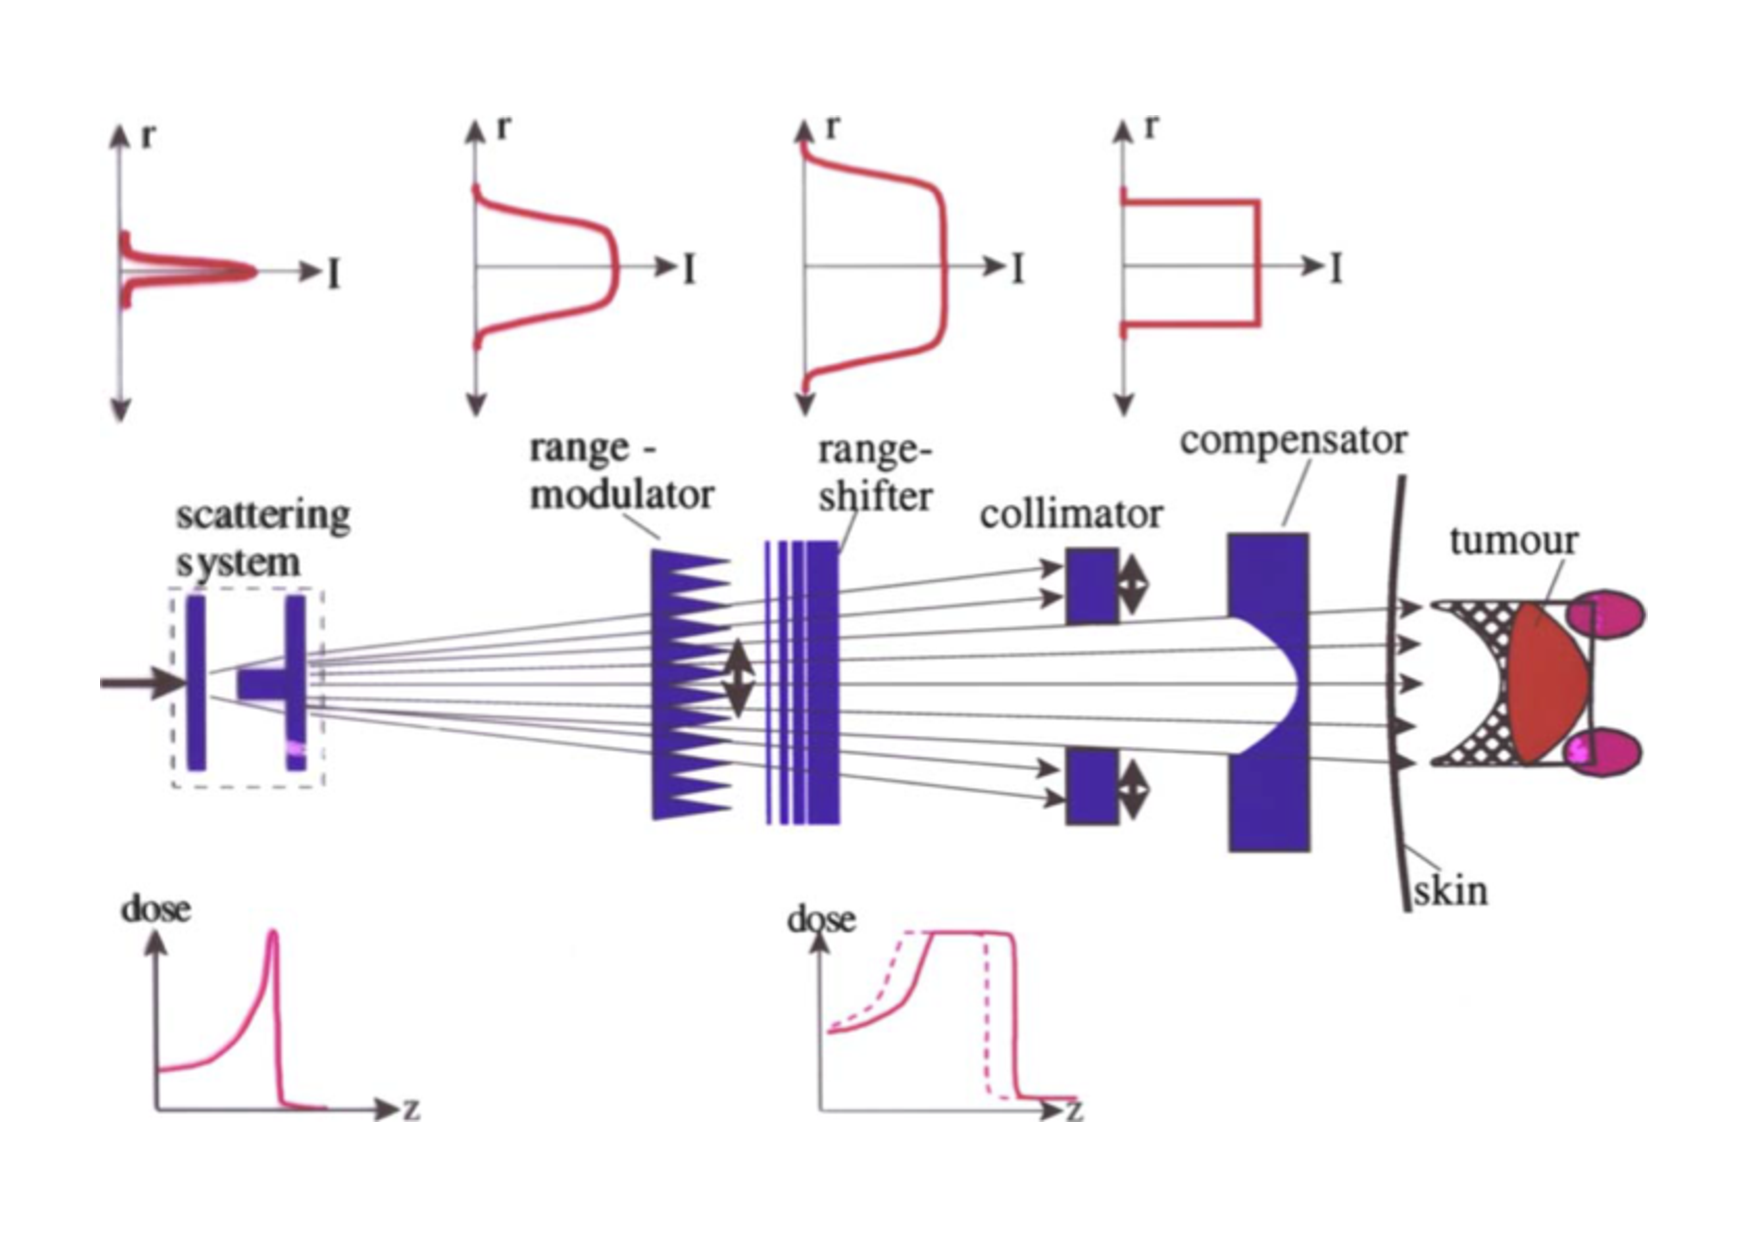
\includegraphics[width=0.7\textwidth]{03_GraphicFiles/chapter1_Introduction/passiveDelivery.pdf}
\caption{Schematic view of a fully passive beam delivery system. In~\cite{Schardt2010}.}
\label{chap1::fig::passiveDelivery}
\end{figure} 

The passive beam delivery technique presents three main disadvantages with respect to the active delivery described in the following. First, the structure of the created \gls{sobp} is fixed and the depth-dose can only be tailored to the distal end of the target volume and not to the proximal end, given the fact that the \gls{sobp} can only be shifted towards the entrance region. This feature automatically leads to a considerable dose given to normal tissues outside the target volume, in particular in the proximal part, as illustrated by the hatched region in \figurename~\ref{chap1::fig::passiveDelivery}. Second, the amount of material inserted in the beam line causes nuclear interactions which lead to the creation of secondary high-\gls{let} fragments (mainly neutrons), affecting the dose delivered to the entrance region. Third, each collimator/compensator are specifically designed for each patient irradiation port, which leads to complex and costly manufacturing for such devices.
The main asset of passive beam delivery is that the whole target volume is irradiated at once, which leads to shorter irradiation times. This last point is quite important for the irradiation of large \glspl{ptv}.

When the beam is produced with a synchrotron, \myMarginnote{Active beam scanning} the possibility to switch the energy from pulse to pulse makes feasible an active target scanning and beam range adaptation. Active beam delivery is also possible with cyclotron-accelerated beams, but the beam energy is modulated with degrading passive elements, and a spectrometer is needed for energy selection, at the cost of an important intensity reduction. The active beam delivery systems exploit the electrical charge of the accelerated particles to deflect the beam laterally through magnets and perform a scan of the defined treatment field. A schematic view of an example of active delivery system is provided in \figurename~\ref{chap1::fig::activeDelivery}. The target volume is divided into iso-energetic layers which are irradiated sequentially by deflecting the beam with dipoles in order to fully cover a grid of pre-defined voxels.              

\begin{figure}[!htbp]
\centering
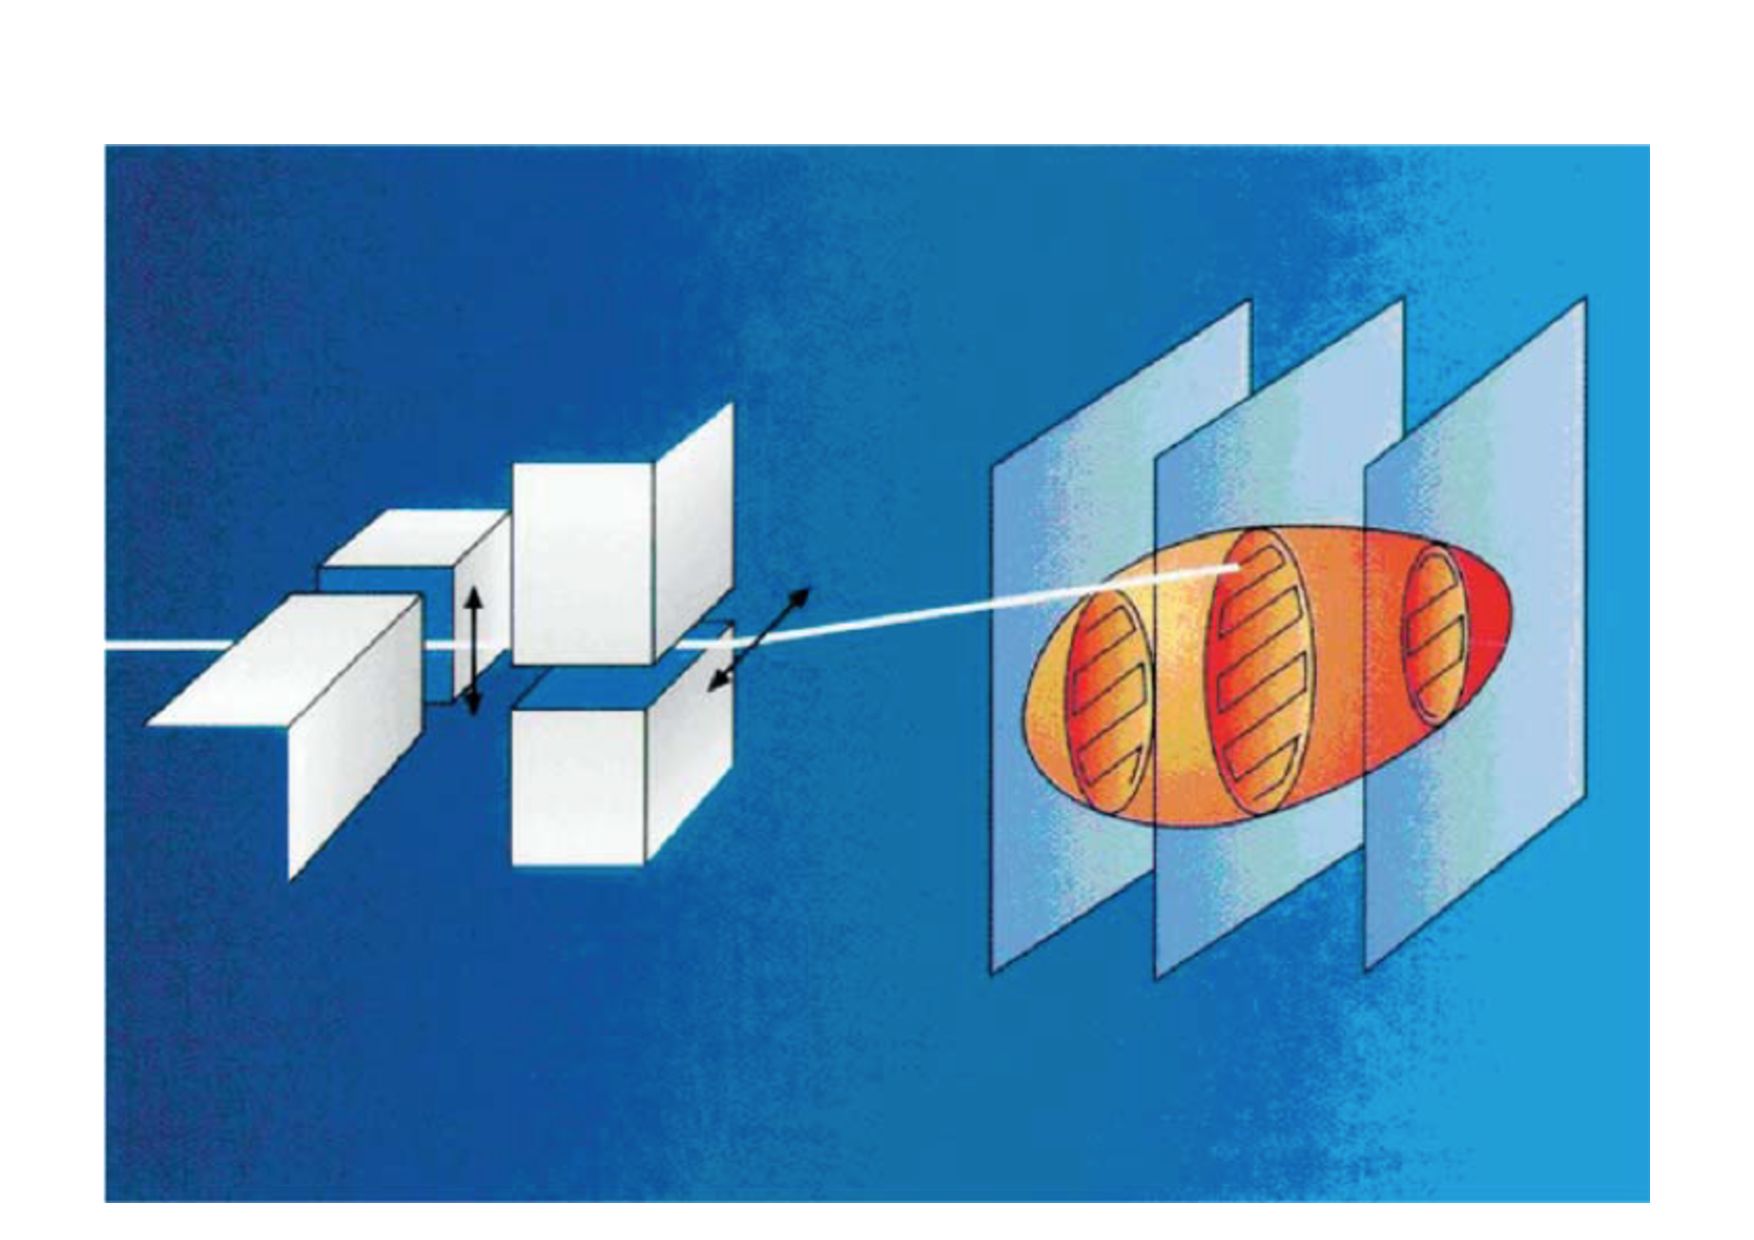
\includegraphics[width=0.7\textwidth]{03_GraphicFiles/chapter1_Introduction/activeDelivery.pdf}
\caption{Schematic view of a fully active beam delivery system. In particular, here the \gls{gsi} raster scanning system is depicted. In~\cite{Schulz-Ertner2006}.}
\label{chap1::fig::activeDelivery}
\end{figure} 

Even if this approach is demanding from the accelerator performance point of view, it brings several advantages with respect to a passive one: there is no need for patient specific equipment like collimators and compensators, and any volume can be in principle covered with a conformal dose; the dose can be adapted on a single voxel basis; the material in the beam line close to the patient is minimized so that the production of secondary particles is strongly reduced. 
With such a delivery system, the term \gls{impt} has been introduced, in analogy to the \gls{imrt} techniques applied in standard photon radiotherapy. Indeed, the \gls{imrt} exploits multi-leaf collimators to tailor the beam to the target, so that it results to be similar to ion passive delivery systems. In photon therapy, the beam modulation on a single spot basis is possible with cyber-knife machines~\parencite{Srivastava2015}.   
The first so-called \enquote{spot-scanning} system was introduced at \gls{nirs}, already in the early 80's~\parencite{Kanai1983}. This first experience was soon followed by a pilot project of spot-scanning at \gls{psi}~\parencite{Pedroni1995} and by the realization of a fully 3D scanning beam system at \gls{gsi}, where the \enquote{raster-scan} technique is implemented~\parencite{Haberer1993} (with the beam moved from one voxel to the next one with no interruptions, and all points in an iso-energy slice connected together in a dense grid). 
Nowadays, various companies are offering commercial scanning beam system solutions, so that a rapid spread of this convenient technique is foreseen for the next years. The counterpart of the active scanning system is a relatively slow delivery of a given dose in a large tumor volume (minimum 1~ms per spot - ~\cite{Durante2016}), which can be more rapidly covered by passive delivery approaches.  
 
We described till here static beam configurations, \myMarginnote{Rotating-gantries} with a fixed irradiation position. In the clinical routine, in order to further improve the target volume-to-healthy tissue dose ratio, various beam penetration angles can be foreseen, similarly to standard photon therapy (even if a reduced number of different angles is required). In addition to this, deep-seated tumors close to \glspl{oar} can require specific irradiation angles to be treated with the desired safety margins. In order to achieve this goal, two approaches are possible: rotate the patient or rotate the beam line. 
Even if the patient rotation solution has been explored in the past, several reasons are in favor of a fixed supine position, with only horizontal rotations allowed: the supine position is in compliance with the pre-treatment imaging (\gls{ct} scan) used for treatment planning (see section~\ref{chap1::subsec::treatmentPlan}); a patient rotation necessarily leads to organ motion which is undesired; the supine position is more reproducible in the different treatment fractions. As a consequence, rotating gantries have been developed to allow for the beam line displacement.    
The electron linacs employed in conventional radiotherapy are generally mounted on gantries which can rotate 360 degrees around the patient couch to select the optimum beam direction. 
Likewise, in hadrontherapy, rotating gantries solutions have been designed for both protons and heavier ions. In contrast to the compact gantries used in standard radiotherapy, the high beam magnetic rigidity (defined as the product of the bending radius and the required magnetic field strength, equal to the ratio of momentum to charge of the particles) is a constraint on the size of these structures for proton therapy, and, much more, for heavier ion therapy. In general, the beam is first deflected away from the extraction axis, and then bent back to the patient direction with several dipoles. Moreover, quadrupoles are use to optimize the beam focusing before the treatment room. A scheme of a standard gantry design is given in \figurename~\ref{chap1::fig::schemeGantry}. As already mentioned in section~\ref{chap1::subsubsec::accelerators}, the first gantry for protons was installed at the Loma Linda University Medical Center in 1990, followed in 1996 by the first one in Europe at \gls{psi} in 1996, which also included an upstream scanning system~\parencite{Pedroni1995}. At present most of proton therapy centers are equipped with at least one rotating gantry.
The huge dimensions imposed by the carbon ion beam rigidity (three times bigger rigidity for 5000~MeV carbon ions with respect to 200~MeV protons) limited the implementation of such a technology in carbon therapy centers, while different technical solutions have been explored. As an example, at \gls{himac}, in a single treatment room the beam can be delivered to the patient via an horizontal and a vertical line, for the sequential treatment from different angles. The first rotating gantry system for heavy ions was installed at \gls{hit} and is now in operation: the diameter is of 13~m, for a total weight of about 700 tons (see \figurename~\ref{chap1::fig::HITgantry}).

 \begin{figure}[!htbp]
 \begin{subfigure}[t]{.49\textwidth}
\centering
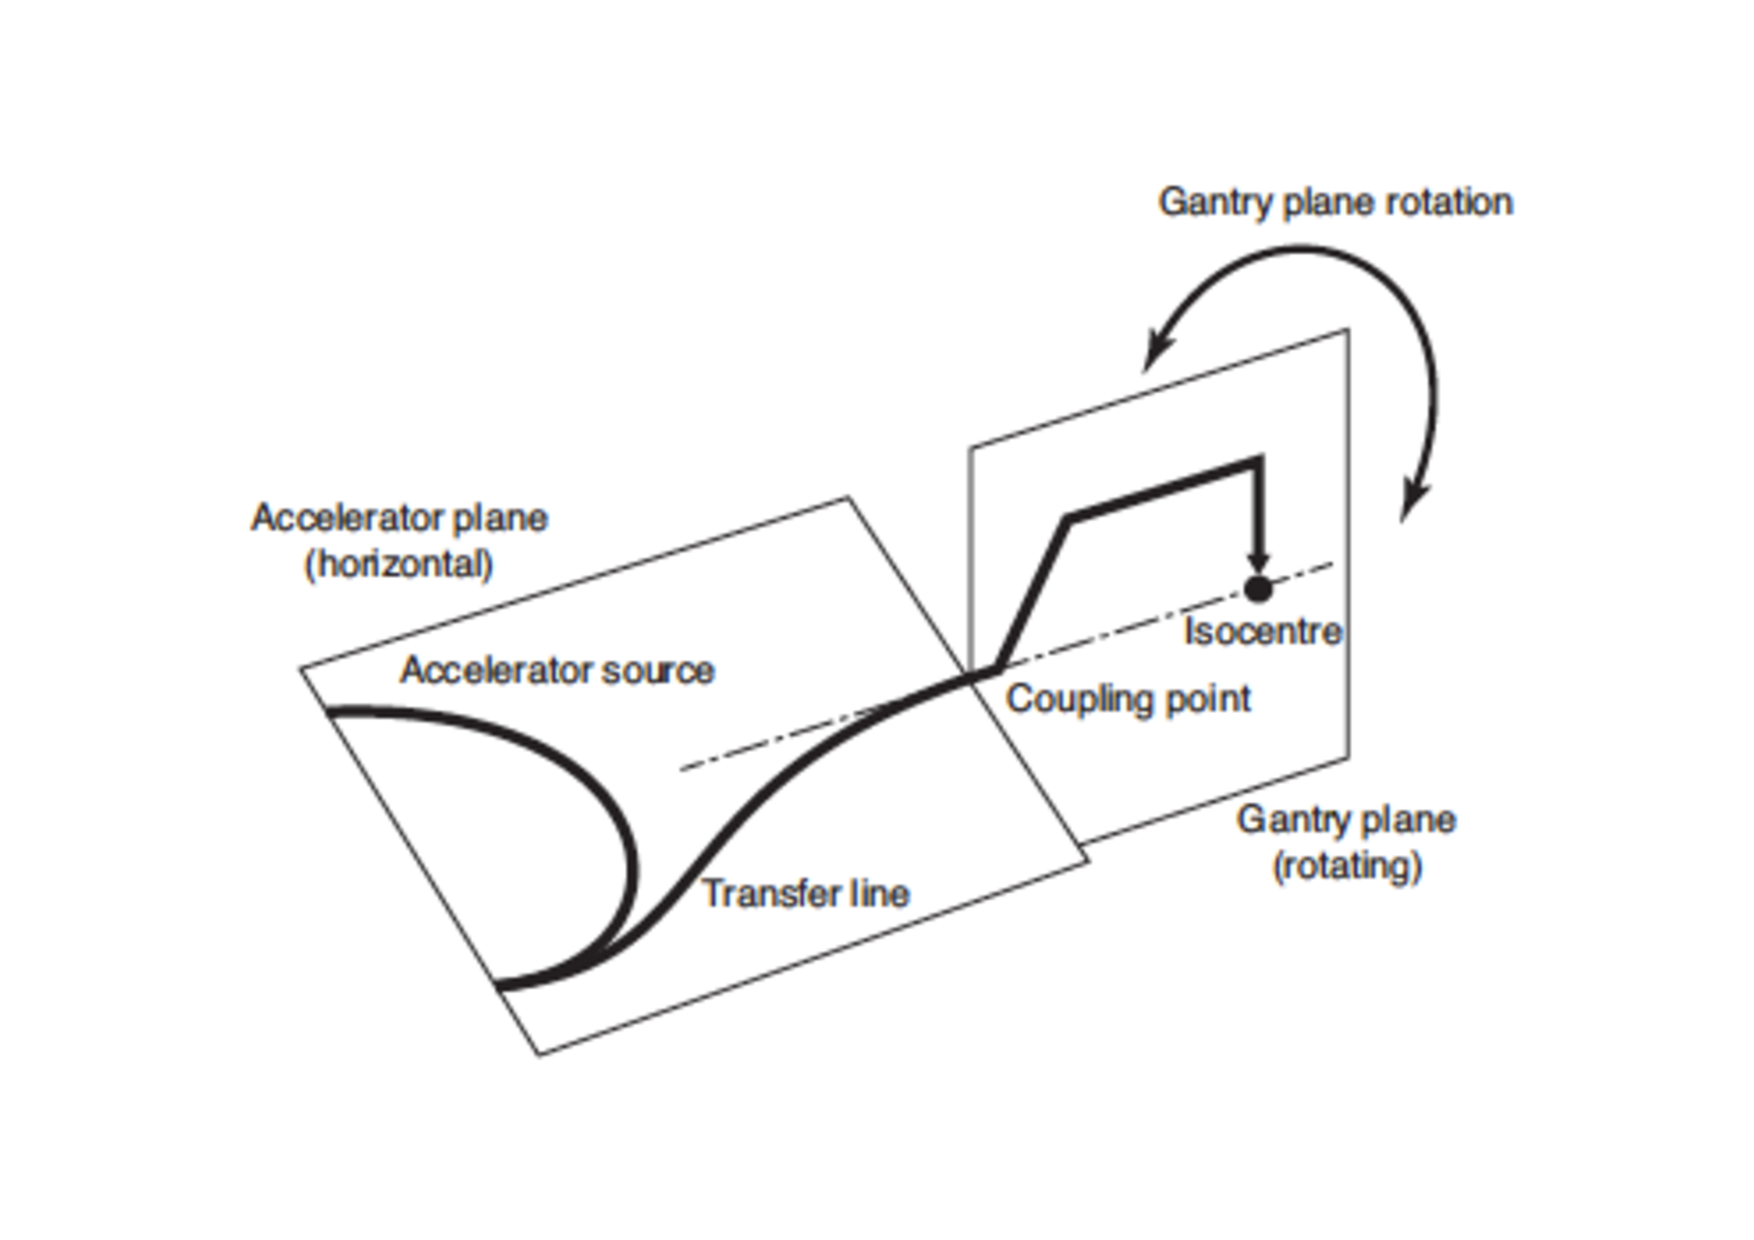
\includegraphics[width=0.92\linewidth]{03_GraphicFiles/chapter1_Introduction/scheme_gantry.pdf}	
\caption{Schematic design of a rotating gantry installed in a particle therapy center. In~\cite{Owen2014}.}
\label{chap1::fig::schemeGantry}
\end{subfigure}
 \begin{subfigure}[t]{.49\textwidth}
\centering
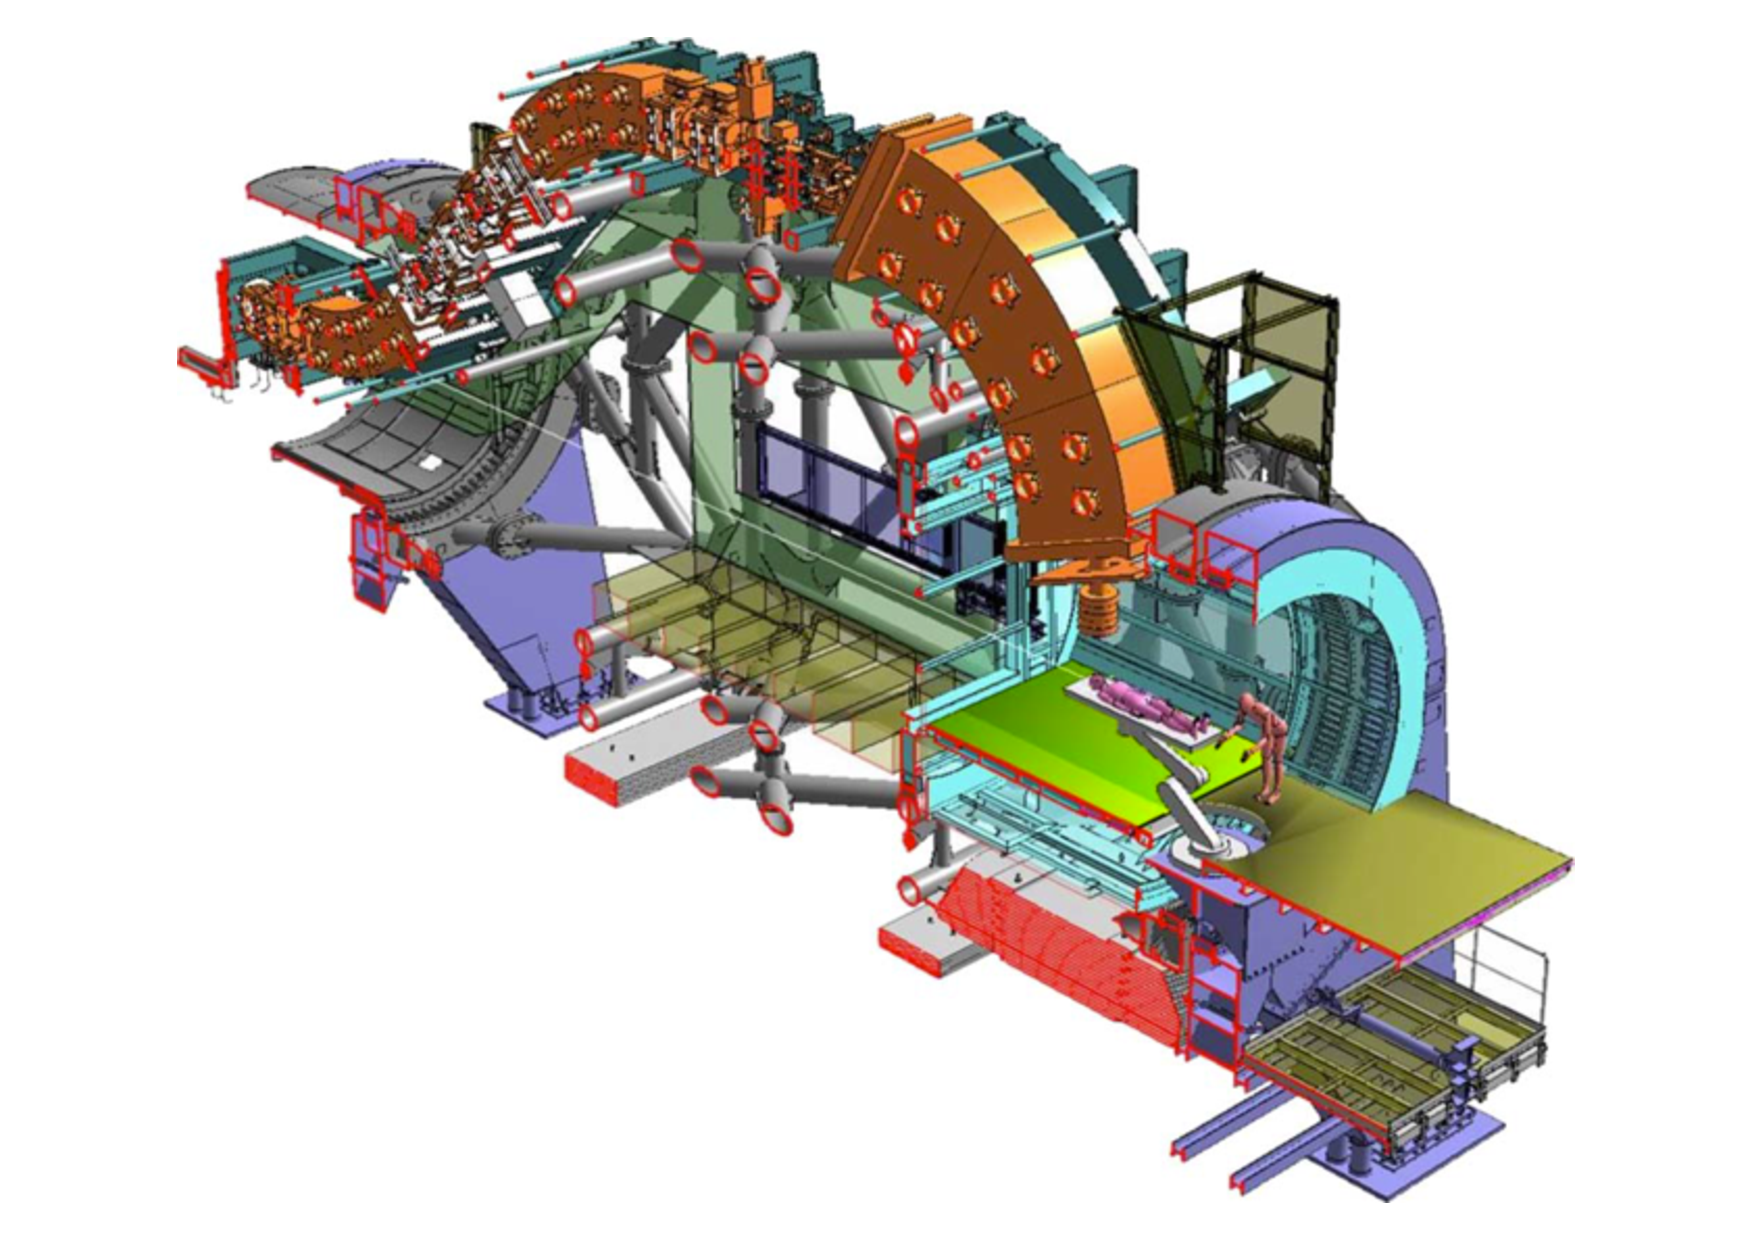
\includegraphics[width=0.99\linewidth]{03_GraphicFiles/chapter1_Introduction/HITgantry.pdf}
\caption{Scheme of the \gls{hit} ion rotating gantry. In~\cite{Schardt2010}.}
\label{chap1::fig::HITgantry}
\end{subfigure}
\caption{Schemes of a standard gantry design (left) and of the carbon-ion rotating gantry installed at \gls{hit} (right).}
\label{chap1::fig::Gantry}
\end{figure}           

Intense research efforts are dedicated to improve the gantry technology, mainly directed towards the implementation of more compact systems equipped with superconducting magnets. A first superconducting carbon ion gantry has been recently installed at \gls{nirs}, and is approximately half size with respect to the German one~\parencite{Iwata2013}.

\subsection{Treatment planning}\label{chap1::subsec::treatmentPlan}

Given the available accelerator and beam delivery system, the best possible treatment features are elaborated by the treatment planning process, which combines the clinical information about the patient with the physical an biological aspects of particle therapy. 
The treatment planning is always patient and disease-specific, and is based on imaging techniques aiming to provide the physicians with the data necessary to delineate the target volume and the surrounding \glspl{oar}. The minimal approach is represented by a pre-treatment x-ray \gls{ct} scan, providing quantitative information about the anatomical structures via photon attenuation images. As briefly outlined in the previous paragraph, it is important to record the pre-treatment images in the same conditions (patient position, fixation structures, etc.) later applied in the treatment itself. Complementary imaging devices, such as \gls{mri} and \gls{pet}~\parencite{Levy2007}, are often used in combination with \gls{ct} to improve the target definition quality, mainly in case of proximity with \glspl{oar}.
In addition to the target delineation, the physicians are also in charge of the therapy prescription, which includes the total dose to be delivered to the \gls{ptv}, the dose limits for the surrounding tissues, and the fraction planning.
All the listed information are the input for the \gls{tps} \myMarginnote{Treatment-Planning System}, which makes the connection between the prescribed dose distribution and the beam acceleration and delivery devices. The physicists and clinicians use the \gls{tps} to define all the treatment beam-specific features such that the clinical prescription is satisfied at the maximum extent. The software output details the beam entrance ports to be used (in terms of gantry positions, if a gantry is available), the beam ranges and intensities, the irradiation scheme in terms of dose-per-voxel, and, more generally, the expected dose distribution in the patient, which allows to quantify the ~\gls{tcpr} and the probability of complications to
the normal tissues.
As the whole planning process is based on x-ray \gls{ct} scans,  \myMarginnote{From Hounsfield units to relative stopping power} providing photon beam attenuation images, a relationship between the \gls{ct} values and ion~\gls{rsp} is needed. The \gls{ct} values are expressed in \gls{hu}, defined as

\begin{equation}
\mathrm{CT\,value}(\vec{x}) =1000 \times \frac{\mu (\vec{x})-\mu_{W}}{\mu_{W}}
\label{chap1::eq::HU}
\end{equation}
where $\vec{x}$ is the considered location, $\mu(\vec{x})$ the x-ray absorption coefficient in tissue, $\mu_{W}$ the one in water as reference. Water is always used as reference medium, in particular through the concept of \gls{wepl}. There is not a functional relationship between the two quantities, and systematic studies have been carried out at \gls{psi} for protons~\parencite{Schneider1996, Schaffner1998}. For carbon ions, similar investigtions have been performed at \gls{nirs}~\parencite{Matsufuji1998, Kanematsu2003} and \gls{gsi}~\parencite{Jakel2001, Rietzel2007}, and experimental verification has been obtained via measurements on animal tissues. In \figurename~\ref{chap1::fig::HU} the data of a look-up table for the conversion of \gls{hu} into carbon ion \gls{wepl} are plotted in the \gls{hu} range of relevant biological tissues.

 \begin{figure}[!htbp]
\centering
\includegraphics[width=0.6\linewidth]{03_GraphicFiles/chapter1_Introduction/HounsfieldUnits.pdf}	
\caption{Hounsfield look-up table for carbon ion treatment planning, based on the data collected at \gls{gsi} and reported in~\cite{Jakel2001}. In~\cite{Rietzel2007}.}
\label{chap1::fig::HU}
\end{figure}
 \begin{figure}[!htbp]
\centering
%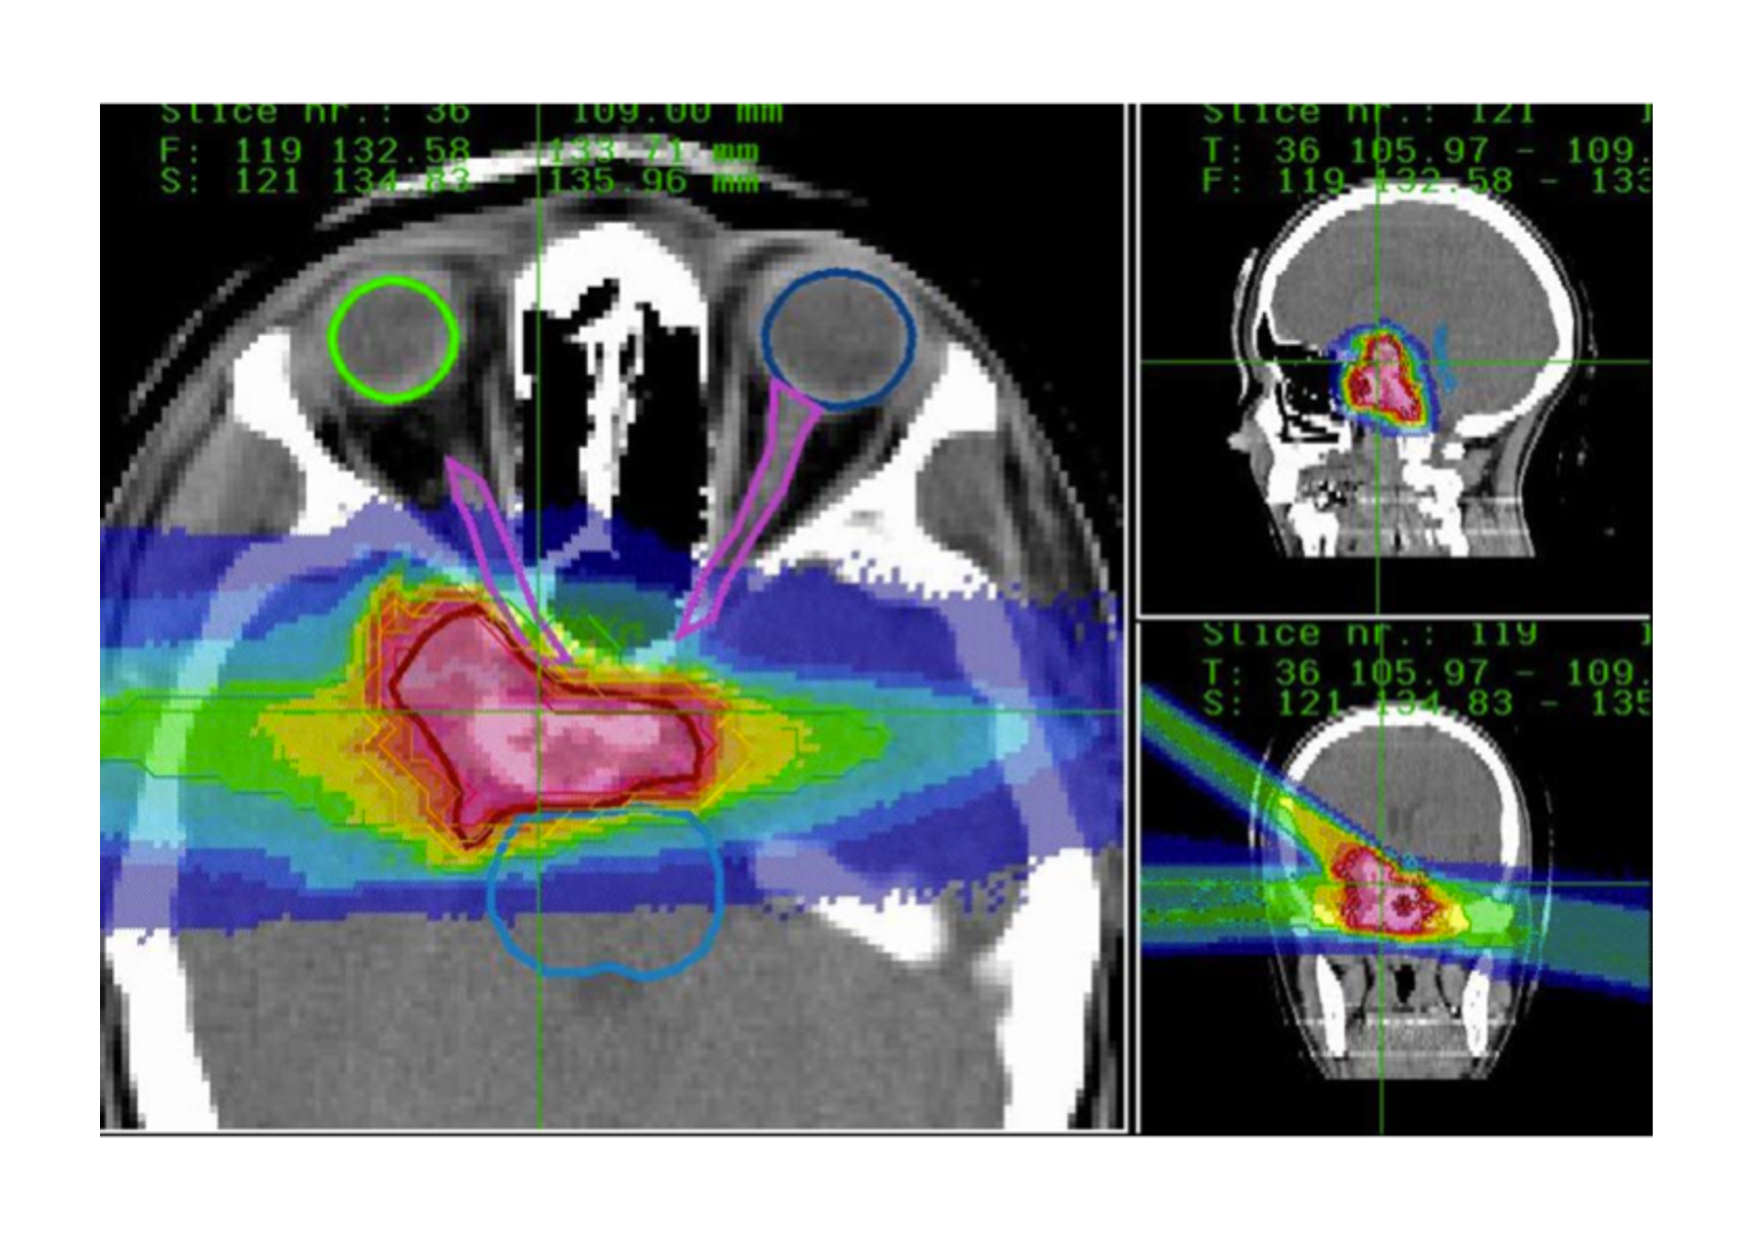
\includegraphics[width=0.92\linewidth]{03_GraphicFiles/chapter1_Introduction/TRIPplan.pdf}
%\caption{Biologically effective dose distribution for the treatment of a skull base tumor, optimized with the \gls{tps} TRiP~\parencite{Kramer2000} at \gls{gsi}. In~\cite{Schardt2010}.}
%\label{chap1::fig::tps_plan}
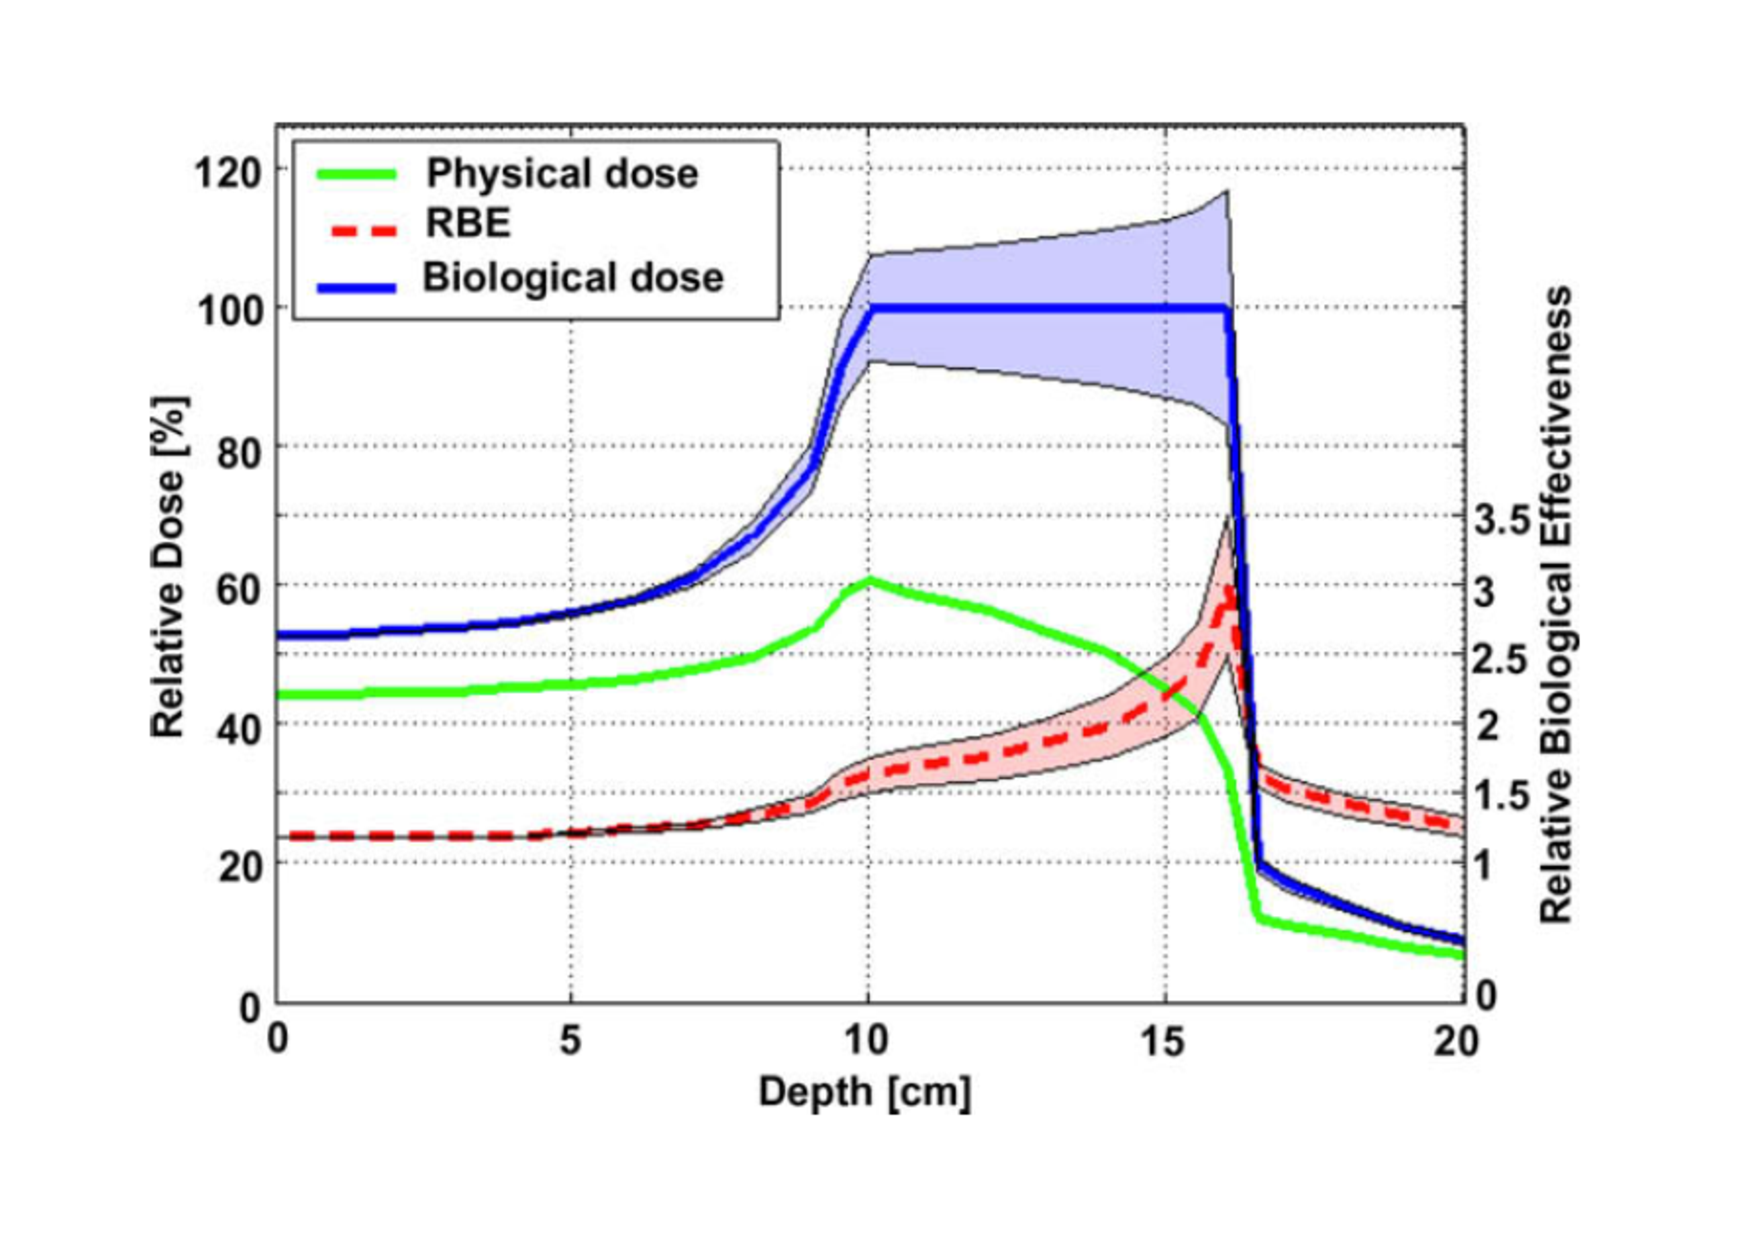
\includegraphics[width=0.6\linewidth]{03_GraphicFiles/chapter1_Introduction/rbeWeightedDose.pdf}
\caption{Comparison of physical (green solid line) and biological (blue solid line) dose for a 290~MeV $^{12}$C ion beam with a 6 cm SOBP for a maximum \gls{rbe} of 3.0. The \gls{rbe} varies in the range 2.5–3.5 and an uncertainty band is sketched to represent the biological dose possible variation due to the selection of the \gls{rbe} value (dashed-red line). In~\cite{Suit2010}.}
\label{chap1::fig::rbeDose}
\end{figure}
%\caption{The treatment planning system process is based on anatomical information about the patient, given by \gls{ct} scans, and physician treatment prescription. The \gls{ct} values must be converted to \gls{rsp} and tabulated experimental data are used (left), while biological dose calculation models are applied to optimize the biological dose distribution to be delivered during the treatment (right), with the related uncertainties connected to the \gls{rbe} variations.}
%\label{chap1::fig::TPS}
%\end{figure}           

The conversion factors are tabulated and implemented in the main \glspl{tps}, but several studies are still ongoing in order to optimize the calibration accuracy (as an example, see~\cite{Inaniwa2018}). As highlighted in several research works, this is one of the main sources of uncertainty affecting proton and carbon ion range prediction and, so, treatment precision. Possible investigated solutions to reduce systematic uncertainties in the \gls{rsp} determination related to the Hounsfield unit conversion are represented by \gls{pct} and dual energy x-ray \gls{ct}~\parencite{Yang2010}. Further details will be given in section~\ref{chap1::subsec::uncertainty}.
In addition to the beam range determination, \myMarginnote{Biological dose modeling} the \gls{tps} software must also deal with biological dose calculations. Indeed, as highlighted in section~\ref{chap1::subsec::bioEffects}, charged particles differ from photons in their radiobiological properties and effects. Notwithstanding the 10-20\% \gls{rbe} variations verified for protons with varying \gls{let} along the path in the patient tissues, a practical constant value of 1.1 is generally used in clinics~\parencite{Paganetti2002, ICRU2007}. This value corresponds to the average \gls{rbe} at mid \gls{sobp} overall dose levels. In the distal section of the Bragg peak, an higher \gls{rbe} has been verified; this effect slightly affects the dose profile fall-off in protontherapy and is not modeled in the present planning systems. As mentioned in section~\ref{chap1::subsec::bioEffects}, several studies are ongoing in the last years with the aim of optimizing the biological models and applying a variable proton \gls{rbe} in clinics, and the topic is still open to discussion in the expert community~\parencite{Paganetti2013, Paganetti2014, Unkelbach2018, Luhr2018, Willers2018}. A different approach must be applied to heavy ions (carbon ions in particular), given the much stronger dependence of their \gls{rbe} on the various parameters listed in section~\ref{chap1::subsec::bioEffects}. Focusing on carbon ions, treatment plans are generally optimized using the so-called \gls{rbe}-weighted dose, calculated according to verified models based on experimental data. In \figurename~\ref{chap1::fig::rbeDose}, the physical and biological doses absorbed during a carbon ion beam irradiation with a \gls{sobp} are compared and the \gls{rbe} variation along the beam path is also reported, together with the estimated uncertainties which also affect the \gls{rbe}-weighted dose evaluation. For this purpose, two main models are nowadays implemented in clinical practice. On one side, the Japanese centers use a model developed at \gls{nirs}, based on in vitro cell killing experiments on human salivary glands and neutron irradiation experience gathered at \gls{himac}, as well as on the application of the \gls{lq} model~\parencite{Matsufuji2007}. Recently, a modified \gls{mkm} has been introduced in order to optimize the plans to active scanning with ion beams~\parencite{Inaniwa2015}. On the other side, a specific biophysical model has been developed in Germany at \gls{gsi}, called \gls{lem}, and it is now used in the clinical centers in Germany, Italy and China. Its main idea is to transfer known cell-survival data for photons to ions, assuming that the difference in biological efficiency arises only from a different pattern of local dose deposition along the primary beam~\parencite{Kramer2000, Jakel2001a}.
The two models have been verified to give comparable results, in agreement with the measured \gls{rbe}, with in-vitro experiments on mice cells~\parencite{Uzawa2009}, while different predictions are obtained when different treatment schemes on different tissues are studied~\parencite{Fossati2012, Steinstrater2012}. Besides, the NanOx model (described in ~\cite{Cunha2017}) is being developed in order to address some of the flaws of the \gls{lem} and \gls{mkm}. The model is able to predict cell survival with good agreement to experimental data, and its parameters are under study for optimization~\parencite{Monini2018}. The definition of a common effective dose prediction method is ongoing: this will allow for comparative studies of clinical results and for an improved collaboration of the few ion treatment centers operating all over the world.
These biological models are applied for the planning of active scanning carbon ion treatments, for which the target volume is previously divided into slices: the dose is then optimized for iso-range slices. In contrast, for proton passive beam delivery systems, the plan optimization is generally reduced to the study and production of the patient-specific beam modulators. 
In the future, biology-guided forms of proton therapy can be foreseen; the \gls{rbe} variations, instead of being an issue for which corrections are needed to the treatment planning, could be used to the treatment effectiveness advantage.  
Focusing on the possible direction of improvements in the future of treatment planning \myMarginnote{Treatment of moving organs}, the research efforts are concentrated in the last years also on another fundamental topic: the treatment of moving organs. It is clear that the well-defined ion range and narrow dose peak make ion treatments potentially more sensitive to inter- and intra-fractional organ motion, as highlighted in~\cite{Phillips1992, Bert2008, Engelsman2013} and~\cite{Thornqvist2013}, as an example. Concerning the organ displacement between following fractions, it can be corrected by more frequent imaging scans, ideally a new one before every treatment fraction, in order to adapt the treatment planning to weight variations, target size modifications and similar anatomical effects. The organ movement caused by the respiratory cycle requires more complex strategies to be taken into account for the treatment plan and delivery. The respiratory motion patterns are genarally complex and not regular, involving translational and rotational displacements. Several strategies to mitigate the effect of organ motion are being investigated, some of them directly coming from the experience acquired in \gls{imrt}. As well summarized in~\cite{Schardt2010}, among these strategies it is worth to mention rescanning of repainting techniques, based on the average effect of several irradiations with reduced beam fluence on the same iso-range slices; gating techniques, which aim to correlate the irradiation active time to a continuous monitoring of the respiration cycle; tracking, which requires a 3D compensation of the target motion in real-time, particularly adapted for scanning techniques. A further step will be the real time monitoring of moving organs by means of external markers linked to biomechanical modelling of internal organs~\parencite{Manescu2013}. Some of the cited techniques, or combinations of them, are being tested and are now at the validation stage, but there is still wide room for improvements towards the application of 4D treatment planning~\parencite{Graeff2013, Bert2017}. Further information about this topic  can be found in a recent review by Kubiak~\parencite{Kubiak2016}.    
Range predictions, biological modeling and organ motion are only some of the sources of uncertainties affecting the planning and delivery of ion therapy treatment, detailed in section~\ref{chap1::subsec::uncertainty}; for this reason, safety margins \myMarginnote{Safety margins} are applied in clinics for the definition of the irradiation target volume and the quantification of the planned dose. In the actual clinical routine, the \gls{ptv} is a geometrical extension of the so-called \gls{ctv} and is delineated in order to account for treatment uncertainties. Safety margins are also applied in standard x-ray therapy~\parencite{McKenzie2000}, where under- or over-shooting errors have limited effects with respect to ion beam therapy. As highlighted in~\cite{Albertini2011}, the application of safety margins is useful to improve the treatment plan robustness in case low dose gradients are applied, while the effect results marginal for highly modulated \gls{impt}. At present, in order to account for the overall effects of all sources of uncertainties in the range prediction (\gls{mcs}, beam energy straggling, imaging tools accuracy and calibration, biological effects, patient positioning and organ motions), margins up to 3.5\% + 3~mm can be applied around the \gls{ctv}~\parencite{Paganetti2012}, mainly based on Monte Carlo or analytic dose calculations which result in clinically compatible predictions. 

In the following paragraph, the uncertainties related to ion therapy treatment are discussed in details, with particular care devoted to possible clinical solutions.

\subsection{Ion beam therapy uncertainties and treatment monitoring}\label{chap1::subsec::uncertainty}
Heavy charged particles are suitable for cancer radiation therapy given the better achievable dose conformity and the reduced energy deposit in tissues surrounding the target with respect to standard photon treatment techniques. These advantageous features directly derive from the nature of ion interactions in matter, described in section~\ref{chap1::subsec::Physics}, which determines a peculiar depth dose profile characterized by a finite range and a energy deposit (dose) peak (Bragg peak). In order to accurately predict the ion range and, more generally, the dose distribution delivered during a clinical treatment, all the possible ion interactions in matter must be considered. This prediction is associated with important uncertainties due to imaging precision, patient setup, anatomical variations and motions, beam delivery system accuracy, dose calculation approximations and biological considerations~\parencite{Paganetti2012}. Ideally speaking, a perfect knowledge of the beam and target structure and perfect evaluation of all the parameters involved in the dose determination would result in the optimal way to treat a deep-seated tumor, with a reduced dose delivered to the surrounding healthy tissue (even close to \glspl{oar}) with limited fields of irradiation, and a dose accurately concentrated to the tumor volume. The actual clinical routine must face limitations in beam production and control as well as in patient composition evaluation, which causes the need for approximated treatment planning and the setup of treatment safety margins (see section~\ref{chap1::subsec::treatmentPlan}), limiting the full exploitation of this treatment technique potential. In this section, an overview of the different sources of uncertainties affecting ion therapy treatments is given, and the solutions, already implemented or under study, are presented, with particular attention focused on ion range monitoring techniques, main topic for this thesis.
All the mentioned sources of uncertainties associated to hadrontherapy treatment converge in a significant spread in the beam effective range with respect to the predicted one. Treatment planning systems are able to accurately model range straggling and \gls{mcs} broadening along the beam path in water~\parencite{Hong1996}, but the prediction accuracy has limitations when translated to patients. As highlighted in~\cite{Schlegel2008}, a precise determination of the primary ion penetration depth is essential in order to rely on particle therapy treatments, much more than for standard photon treatments. The reason is schematically presented in \figurename~\ref{chap1::fig::rangeUnc}.

\begin{figure}[!htbp]
\centering
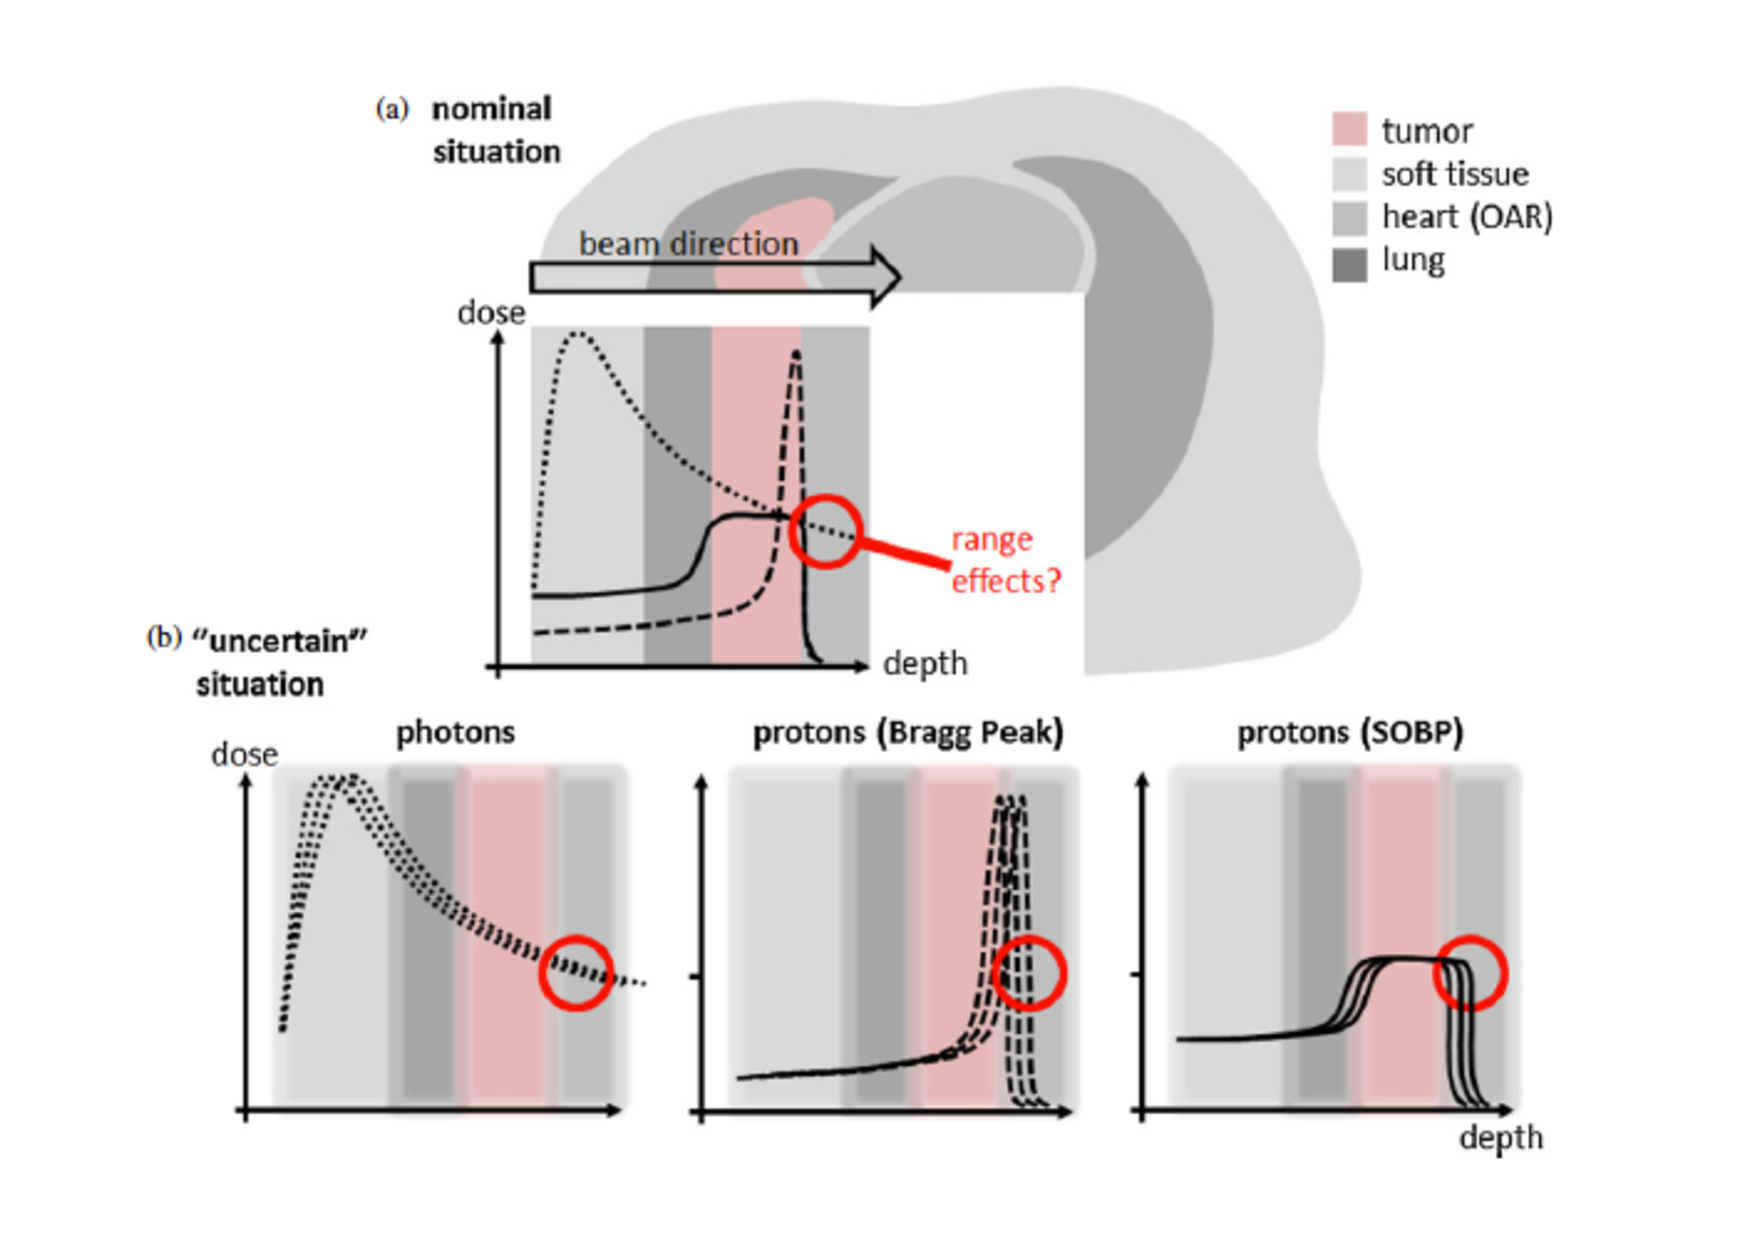
\includegraphics[width=0.7\textwidth]{03_GraphicFiles/chapter1_Introduction/rangeUnc.pdf}
\caption{Schematic view of the potential benefit due to the depth-dose features of protons as compared to photons (a) and influence of range uncertainties on photon irradiation and proton pristine and spread-out Bragg peaks. In~\cite{Knopf2013}.}
\label{chap1::fig::rangeUnc}
\end{figure} 

In the top panel of \figurename~\ref{chap1::fig::rangeUnc} the ideal treatment configuration is shown, with the pristine Bragg peak located at the distal limit of the \gls{ptv} (dashed line) and the \gls{sobp} covering the whole tumor volume (solid line); the two proton irradiation methods are compared to the photon dose profile (dotted line), which releases the maximum of the dose in the entrance region and it is not capable of sparing the tissues surrounding the tumor volume, before and beyond the tumor in the beam direction. In the bottom line of the same figure, the effect of range uncertainties are represented: from left to right, in case of photon dose profile shifts, the modification in the dose delivered to healthy tissues is relatively limited, the main effect being a shift in the dose maximum in the entrance region; for a monoenergetic Bragg peak, a shift in the peak position can result in both an under-irradiation of malignant tissues and a dose maximum located in soft healthy tissues; the same effect is present for the \gls{sobp}, with the only advantage of a reduced under-irradiation of the tumor region. It is clear from this simple case how the extremely sharp dose gradient provided by heavy charged particles must be accurately controlled in order to fully profit of its beneficial effect in treating cancer. 
As mentioned, an exact range calculation is extremely difficult to be obtained in human tissues. As described in section~\ref{chap1::subsec::treatmentPlan}, the treatment planning is at present based on a pre-treatment \gls{ct} scan which is generally acquired only before the first treatment fraction. The \gls{ct} image accuracy is indeed the first source of uncertainty in range calculation \myMarginnote{\gls{ct} uncertainty}. The limitations in the imaging precision (mainly due to image noise - see~\cite{Chvetsov2010}) and the reconstruction artifacts (which can be important in presence of metal implants as verified in~\cite{Jakel2007, Newhauser2007}) already affect the reference data set. Small but not negligible effects are also related to the \gls{ct} resolution~\parencite{Espana2011}. The obtained \gls{ct} data must be then converted from x-ray attenuation values (\gls{hu}) related to water to relative ion stopping power (see section~\ref{chap1::subsec::treatmentPlan}). The conversion is based on calibration curves~\parencite{Schneider1996, Schneider2000}, generally obtained with \gls{ct} scans of tissue phantom materials with known density and elemental composition. These curves are affected by uncertainties, to be added to the fact that the actual conversion is dependent on the material composition: same x-ray attenuation values can correspond to different relative stopping powers, or vice versa. In addition to this, the conversion may depend on the specific \gls{ct} scanner, as shown in~\cite{Ainsley2014}. Several studies have highlighted the magnitude of such uncertainties, which varies, for example, in the range 1-2\% from soft tissues to bones for protons~\parencite{Schaffner1998b}, which is translated in range possible discrepancies of 1-3~mm. Specific studies have also been conducted on animal fresh tissues in order to optimize the \gls{ct} calibration for carbon ion treatments~\parencite{Rietzel2007}. In total, uncertainties of the order of 3\% are generally considered to take into account the described imaging limitations~\parencite{Moyers2001}. It has been proven that dual-energy \gls{ct} can improve material composition information~\parencite{Bazalova2008, Yang2010, Hunemor2014, Wohlfahrt2018} and the resulting range uncertainties can be reduced, in particular for carbon ion therapy~\parencite{Hunemor2014}. A possible solution to further reduce the errors related to the \gls{hu} values conversion is the implementation of direct density measurements techniques, where the treatment beam is also used for imaging purposes giving direct access to stopping power data. This possibility was discussed since the late sixties~\parencite{Koehler1968}, and the technological advancements (mainly in data acquisition systems and detection techniques) recently allowed to obtain promising results in the last years. In addition to the advantageous removal of the data conversion stage, the so-called ion radiography brings other benefits to the treatment side, with the possibility of performing position verification with fast scans just before the treatment delivery~\parencite{Schneider1995}, as well as on the patient side, given the reduced dose necessary for a complete scan with respect to standard x-ray \gls{ct}~\parencite{Schneider1995}. Further details about this imaging technique are given in the dedicated section~\ref{chap1::subsubsec::particleCT}.
Till here the uncertainties directly coming from the treatment planning process have been described, and can be considered as systematic errors, reproduced unchanged for every delivered fraction of the treatment. Conversely, stochastic uncertainties emerge at the treatment delivery level and affect the planned range with random variations. The majority of treatment planning system operating in clinics are based on analytical calculations relying on \gls{wepl} data, not able to account for complex geometries. In presence of tissue inhomogeneities\myMarginnote{\gls{mcs} range degradation}, \gls{mcs} causes what is generally referred to as a degradation in the distal fall-off of Bragg peaks~\parencite{Urie1986}, in particular in proximity of high-density gradients.  Accurate modeling of \gls{mcs} is then strictly required for correct range predictions~\parencite{Schuemann2014}. The patient anatomical configuration\myMarginnote{Patient anatomy changes} plays a major role not only on a single fraction basis, but also in different fractions. Conventional fractionation schemes foresee treatments which can last for several weeks; the patient anatomical characteristics can experience significant changes, such as tumor mass reduction, weight loss or gain~\parencite{Albertini2008}, modifications in the filling of internal cavities. It is clear that such variations introduce further shifts in the predicted ion range, which can be different from fraction to fraction. Moreover, in different fractions, slight differences in the delivered ion energy are possible, with small but not negligible effects. 
Moving on but always referring to static anatomy issues, the patient setup in the treatment room is another source of uncertainty which can cause discrepancies between the planned and the delivered dose distribution, as shown for example in~\cite{Fattori2014}. 
Furthermore, in particular for the treatment of tumors in the thorax, organ motion \myMarginnote{Organ motion dose blurring} is an important source of dose delivery errors. Focusing on lung cancers, which are already difficult to be precisely targeted due to the low lung density (3 times lower than water), the respiratory motions are hard to be modeled and cause an overall blurring of the dose distribution and severe local range variations due to the high-density gradient between dense tumor tissues and low-density lung tissue. Important research efforts are devoted to the optimization of the treatment of moving organs, as explained in section~\ref{chap1::subsec::treatmentPlan}. In particular, for active scanning delivery techniques, potentially powerful if synchronized with the movements of the target areas, an interplay effect involving beam and organ motion can affect the dose homogeneity and must be minimized~\parencite{Dowdell2013, Grassberger2015}.
To conclude the list of source of uncertainties affecting ion beam therapy treatment planning and delivery, it is worth to mention the contribution of biological effects\myMarginnote{Biological effects}. For protons, a generic constant \gls{rbe} value is generally used in clinics to relate proton dose to photon dose, while it has been verified how the biological effectiveness varies along the beam path, in particular at varying \gls{let}. In \gls{sobp}, the increasing \gls{let} at decreasing primary residual energy is compensated by a reduction of the proton fluence, in order to obtain an homogeneous dose distribution. The increase in \gls{let} causes an increase in the \gls{rbe} which is not considered and results in a shift in the biologically effective range, estimated in $\sim$1-2~mm~\parencite{Paganetti2000, Robertson1975, Wouters1996}. Heavier ion therapy planning systems already account for \gls{rbe} variations to prescribe a conformal dose distribution, but the prediction process is not error-free. Moreover, the dose distribution delivered with heavy ion irradiation is also characterized by the peculiar tail beyond the Bragg peak caused by the nuclear interaction fragments; a correct prediction of the nuclear interaction channel becomes significant, and it is at present not accurate enough to point the beam towards critical structures and fully profit of the narrow dose peak.
The optimization of treatment planning system is focused, in the last years, on Monte Carlo-based dose plans, which can reduce the listed uncertainties, and rely on the continuous progress of physical and biological modeling. A complete overview about this topic is given in~\cite{Paganetti2012} for the case of protons. In table~\ref{chap1::tab::uncertainties}, originally presented in~\cite{Paganetti2012} and here reported with the modifications which can be found in~\cite{Durante2016}, the sources of uncertainties in the proton range are reported with an estimate of their relative contribution with and without the application of Monte Carlo optimization techniques.

\begin{table}[!htbp]
\centering
\caption{Estimated magnitude of range uncertainties separated for the various sources, and potential benefit provided by Monte Carlo simulations. The estimates are based on data in~\parencite{Matsufuji1998, Schaffner1998, Chvetsov2010, Bichsel1992, ICRU1993, Kumazaki2007, Espana2010, Urie1986, Sawakuchi2008, Bednarz2010, Wouters1996, Robertson1975, Paganetti2000}. Table reproduced from~\cite{Durante2016}.}
\label{chap1::tab::uncertainties}
\begin{tabular}{m{6cm} P{3.6cm}  P{3.6cm}}
\toprule
\rowcolor{myColorMainA!20} 
\textbf{Source of range uncertainty in the patient}& \textbf{Range uncertainty w/o Monte Carlo (\% or mm)} & \textbf{Range uncertainty with Monte Carlo (\% or mm)} \\
\midrule
\underline{Independent of dose calculation}: & & \\
\hspace{0.2cm} Measurement uncertainty in water & $\varpm$ 0.3~mm & $\varpm$ 0.3~mm \\
\hspace{0.2cm} for commissioning  & & \\
\hspace{0.2cm} Compensator design & $\varpm$ 0.2~mm & $\varpm$ 0.2~mm \\
\hspace{0.2cm} Beam reproducibility & $\varpm$ 0.2~mm & $\varpm$ 0.2~mm \\
\hspace{0.2cm} Patient setup & $\varpm$ 0.7~mm & $\varpm$ 0.7~mm \\
\underline{Dose calculation}: & & \\
\hspace{0.2cm}  Biology & + $\sim$ 0.8\% & + $\sim$ 0.8\% \\
\hspace{0.2cm}  \gls{ct} images and calibration & $\varpm$ 0.5\% & $\varpm$ 0.5\% \\
\hspace{0.2cm}  \gls{ct} conversion to tissue & $\varpm$ 0.5\% & $\varpm$ 0.2\% \\
\hspace{0.2cm} (excluding I-values) & & \\
\hspace{0.2cm}  \gls{ct} grid size & $\varpm$ 0.3\% & $\varpm$ 0.3\% \\
\hspace{0.2cm}  Mean excitation energy (I-values) & $\varpm$ 1.5\% & $\varpm$ 1.5\%  \\
\hspace{0.2cm} in tissues & & \\
\hspace{0.2cm}  Range degradation: complex & - 0.7\%  & $\varpm$ 0.1\%  \\
\hspace{0.2cm} in-homogeneities  & & \\
\hspace{0.2cm}  Range degradation: local lateral & $\varpm$ 2.5\% & $\varpm$ 0.1\%\\
\hspace{0.2cm} in-homogeneities  & & \\
\midrule
\hspace{0.5cm}  \underline{Total} (excluding biology and & 2.7\% $\varpm$ 1.2~mm & 2.4\% $\varpm$ 1.2~mm \\
\hspace{0.7cm} lateral in-homogeneities) & & \\
\hspace{0.5cm}  \underline{Total} (excluding biology) & 4.6\% $\varpm$ 1.2~mm  & 2.4\% $\varpm$ 1.2~mm  \\
\bottomrule
\end{tabular}
\end{table}      

As mentioned in section~\ref{chap1::subsec::treatmentPlan}, the current approach to deal with range uncertainties directly comes from standard x-ray radiation therapy and involves the setting of margins around the target volume. The margins are generally determined analytically and result to be larger in the distal end of the target volume to account for range shifts, while smaller margins are applied laterally to include beam penumbra uncertainties. The field arrangement is another applied mitigation of the problem~\parencite{Lomax2001}, in particular in proximity of \glspl{oar}. For example, lateral fields can be used instead of distal ones. 
Notwithstanding the several solutions used, \textit{in-vivo} verification of the delivered range is still a pressing desire in the clinical community. Standard imaging devices are commonly used to monitor photon therapy treatments, where the delivered beam is not stopped in the patient. On the contrary, ion beams do not exit the patient body, so that monitoring techniques can only be based on secondary radiation or indirect measurements. An exception is represented by implanted devices, proposed for the dose and range measurements, briefly discussed in section~\ref{chap1::subsec::rangeComplTechniques}.
As highlighted in~\cite{Parodi2015}, the monitoring should be ideally in three-dimensions on-line, time-resolved and in real-time, in order to allow for a prompt detection of severe deviations between prescribed and delivered dose, and eventually for the interruption of the beam delivery. A number of different approaches have been proposed in the last years, and significant research efforts are dedicated to this specific point by several groups all over the world. In particular, nuclear reactions products are deeply investigated as a source of information about the beam range. The developed techniques have to be adapted to the present clinical routine, so that the beam features (clinical intensity, time structure, size) and treatment plan characteristics (kind of beam delivery, spot size, irradiation intensity per spot, etc.) must be considered. In the following sections, after a paragraph devoted to charged particle \gls{ct}, the main techniques implemented for ion range monitoring purpose or at present under study are described, and the current available or future instrumentation is presented. In chapter~\ref{chap::2}, the attention will be focused on the detection of \glspl{pg}, central topic of this thesis, and a detailed overview of the state of the art of this particular monitoring techniques is provided.                


\subsubsection{Ion radiography and tomography}\label{chap1::subsubsec::particleCT}

Given the considerable contribution of x-ray \glspl{hu} conversion to ion stopping power to the treatment planning uncertainties, the best solution to overcome this limitation relies in avoiding this conversion step. This can be obtained by directly using high-energy ions to perform patient imaging scan. After the original proposal delineated in the Cormack seminal paper in 1963~\parencite{Cormack1963}, the first studies with protons date back to 1968~\parencite{Koehler1968}, and at the beginning of the seventies the feasibility of this techniques to obtain high contrast images was demonstrated~\parencite{Steward1973, Cookson1974, Cormack1976}. After the first pioneering studies, the developments were almost abandoned in favor of other imaging techniques, in particular x-ray based, providing better spatial resolution with simpler machines~\parencite{Kramer1977}. As a consequence of the present widespread of hadrontherapy and the multiplication of treatment centers, several research groups showed a renewed interests in the field, and various development projects are ongoing in Europe and USA with promising results guaranteed by the significant technological advancements occurred in the last years. To date, most of the experimental efforts have been and are being devoted to proton-based imaging (reviewed for example in~\cite{Poludniowski2015, Bucciantonio2015}), but pioneering imaging experiments with heavier ions were already carried out in the late seventies and eighties~\parencite{Tobias1977, Chu1993}. In recent years, many research groups in Japan and Europe are working on carbon-ion imaging prototypes to be applied in the existing carbon therapy centers. An overview of the ongoing research in the field of proton and ion imaging is given at the end of this section.  
The radiography technique is based on ion beams applied to the patient at higher energy with respect to the treatment ones, which must traverse the body and can be detected on exit to directly retrieve the residual range. In \figurename~\ref{chap1::fig::pCT_design} the design of a standard detection system for ion radiography is sketched. The \gls{mlp} through the patient (phantom) is estimated thanks to two thin tracking detector stages, measuring the primary particle trajectories both entering and exiting the target. The second tracker is followed by a range or energy detector, which measure by complete absorption the residual range or energy of the primary ion. Thanks to the coincidence detection of entrance and exit coordinates and residual energy/range of each primary particle, a density two-dimensional map of the target area can be obtained.  

\begin{figure}[!htbp]
 \begin{subfigure}[t]{.49\textwidth}
\centering
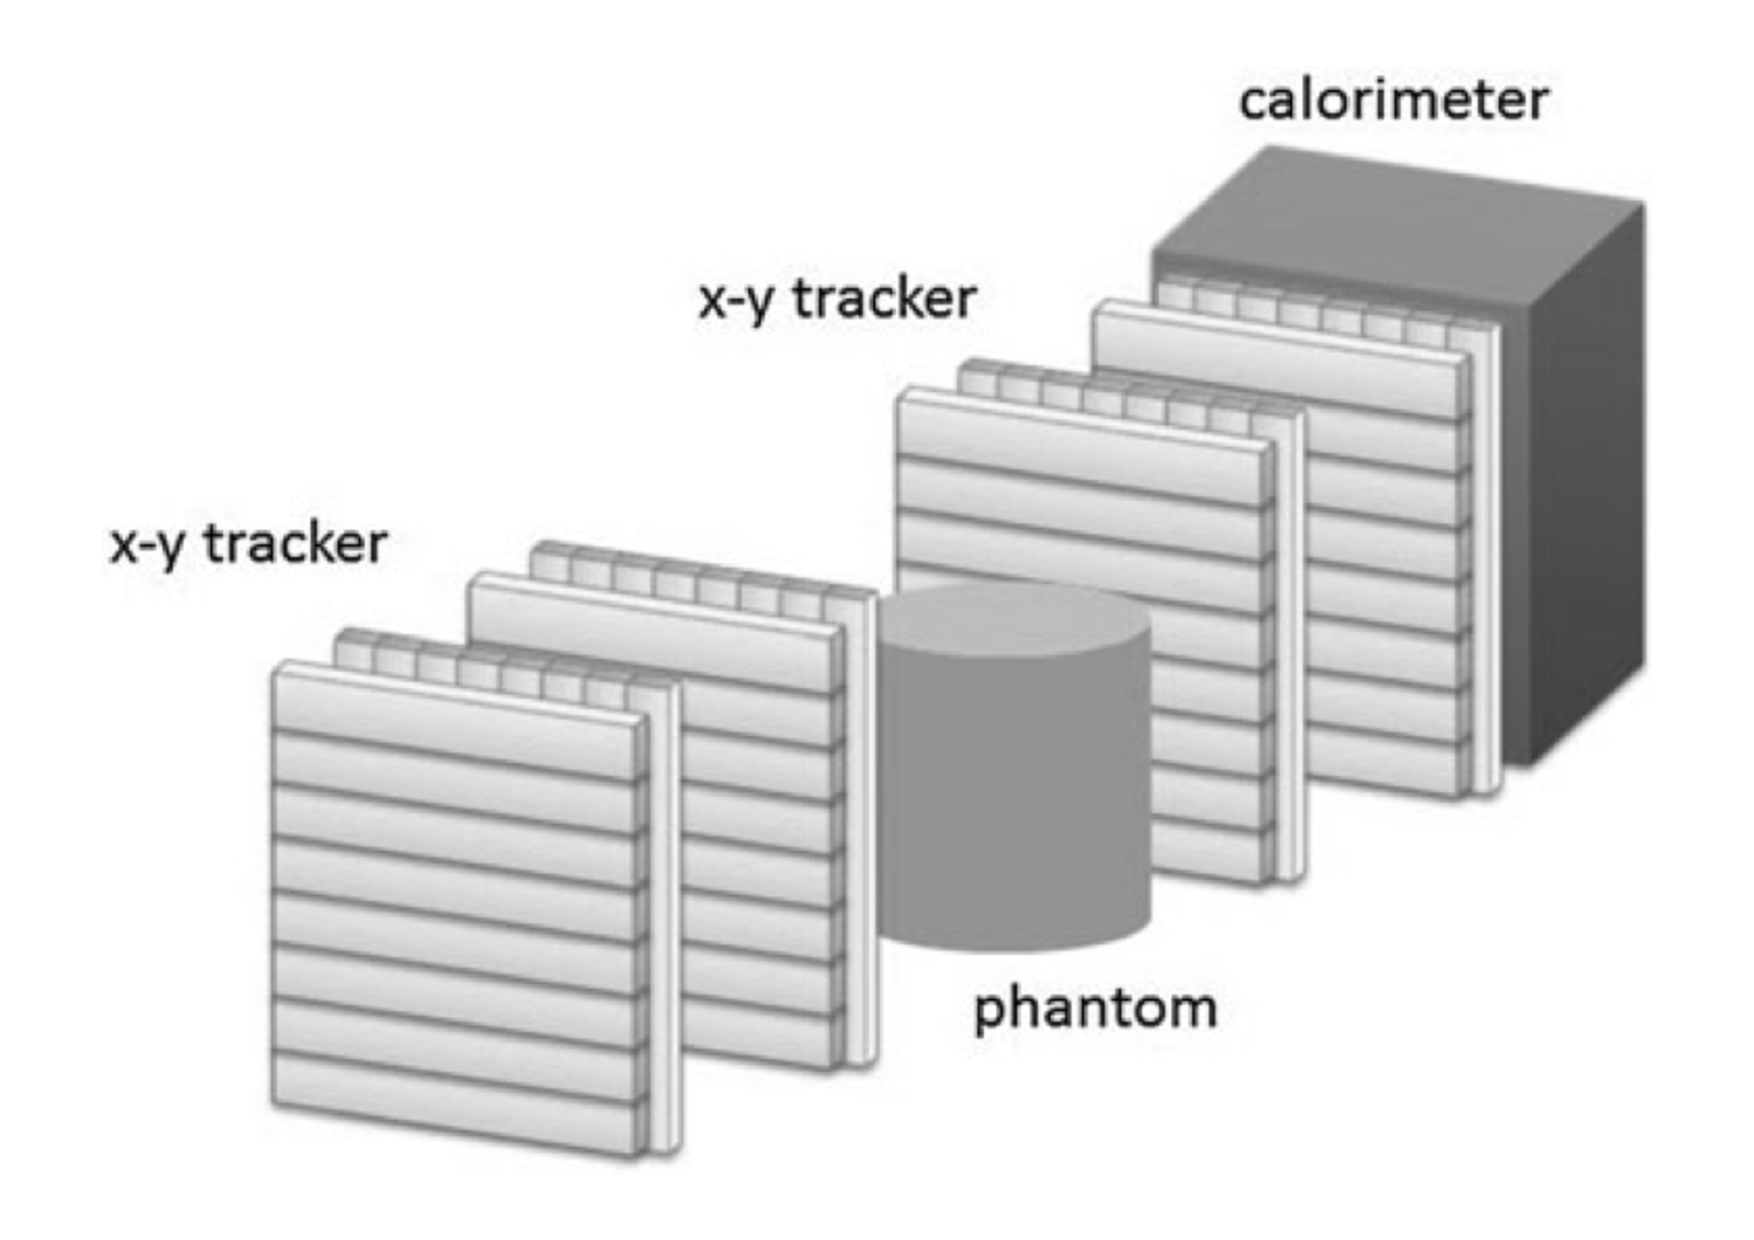
\includegraphics[width=0.9\linewidth]{03_GraphicFiles/chapter1_Introduction/pCT_general.pdf}
\caption{Schematic view of standard ion \gls{ct} detector design. Each primary incoming particle is tracked before the interaction in the patient and at the exit, and its residual energy is absorbed and measured by a calorimeter. In~\cite{Mattiazzo2015}.}
\label{chap1::fig::pCT_design}
\end{subfigure}
\begin{subfigure}[t]{.49\textwidth}
\centering
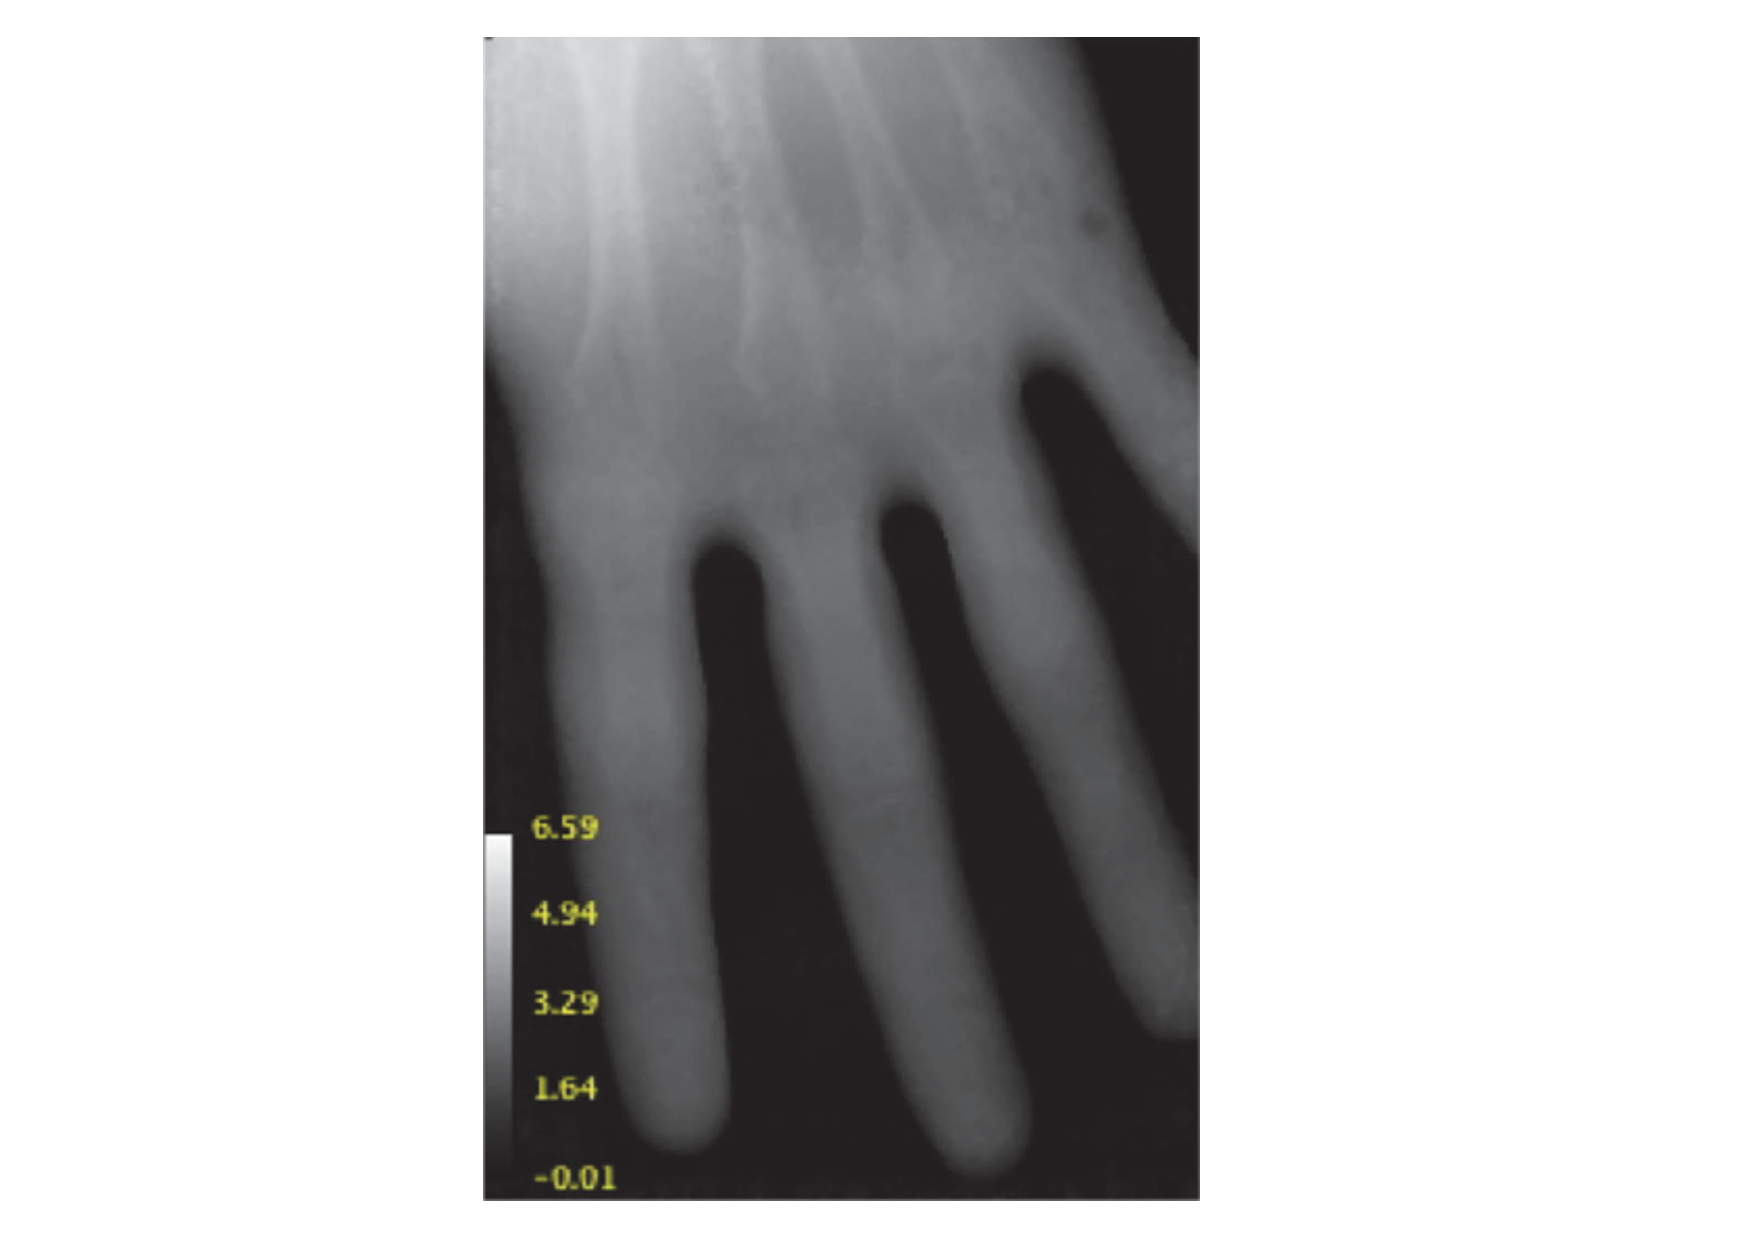
\includegraphics[width=0.92\linewidth]{03_GraphicFiles/chapter1_Introduction/pCT_image.pdf}
\caption{Proton \gls{ct} image of an hand phantom. In~\cite{Plautz2014}.}
\label{chap1::fig::pCT_image}
\end{subfigure}
\caption{Proton and heavier ion radiography and \gls{ct} are under study in the last years as promising techniques for optimizing the treatment planning performance in hadrontherapy. A standard detector design is sketched in the left panel, while the first image of an hand phantom is reported in the right one.}
\label{chap1::fig::ionCT}
\end{figure} 

As mentioned, since all the primary incident particles must completely pass through the target for a residual energy measurements, the beam energy must be higher than the one applied for radiotherapy treatments. In the case of protons, standard clinical accelerators can provide beam at a maximum energy of 230-250~MeV (the projected range of 250~MeV protons in water is $\sim$38~cm - see \gls{nist} tables at~\cite{NISTpstar}), not enough to pass in all directions through the hip region of a typical adult, and far short of the shoulder-to-shoulder distance through a human male. Such energies are anyway sufficient for scanning the head or the lung region for most patients~\parencite{Johnson2017}. The optimal beam conditions for radiography have already been pointed out for protons in one of the first studies about this topic~\parencite{Moffett1975}. At that time, small pencil beams were preferred, with low intensity and limited energy spread. In reality, the beam can be also passively spread to cover the whole detector aperture, or a scanning technique can be used as suggested in the original papers. In addition to the first highlighted advantage of this technique, which provides direct access to stopping power data, there are other factors determining its convenience with respect to x-ray imaging. A dosimetric advantage with respect to x-rays has been already proven in 1975~\parencite{Moffett1975}, and a reduction of imaging dose by a factor 10 to 20 has been reported in ~\cite{Schneider1995}. Recent results showed, for equal density resolution, 50-100 times lower image exposure for protons with respect to x-rays~\parencite{Schneider2004}. Moreover, the low dose enables one to perform proton imaging scans before each treatment fraction: this is potentially very useful for positioning optimization (the scan is performed under the same geometrical conditions as the treatment) and for the detection of anatomical changes, which cannot be included in the present treatment planning, based on a single \gls{ct} scan performed before the beginning of the whole treatment cycle. However, it must be considered that ion radiographies are performed in the same treatment room and couch, limiting the patient flow. Moreover, a major limitation of proton radiography techniques is represented by a poor spatial resolution due to \gls{mcs}, already highlighted in the first publications~\parencite{Koehler1968, Moffett1975}. Several small angle deflections produce uncertainties in the reconstructed trajectories~\parencite{Schneider1995, Schneider2004, Penfold2009}. Heavier ions are less affected by \gls{mcs} in the target, so that better spatial resolution with respect to protons can be achieved, but they suffer from substantial nuclear spallation and the projectile and target fragmentation can add background to the final image~\parencite{Parodi2014}. The helium ions, which already have the advantage of requiring much less energy than carbon ions in order to fully penetrate a phantom, behave more like protons within the phantom, but with significantly reduced scattering and increased spatial resolution. Helium, indeed, appears to be the optimum compromise, even if it is not implemented in clinics for tumor treatments at present. With the increasing diffusion of heavy-ion therapy centers, anyway, we can expect a further development of this field in the next years~\parencite{Parodi2014}.
The described ion transmission imaging method provides two-dimensional information, but it can be extended into 3D with the rotation of the system around the target (or the patient rotation) and the application of tomographic reconstruction. The so-called ion-\gls{ct} makes use of optimized \gls{fbp} methods or \glspl{art} to obtain 3D patient images by combining various data sets from different angles.
At present, ion transmission imaging for both radiography and tomography is not yet clinically implemented, but a number of research groups conducts instrumental development campaigns to produce prototypes to be tested in clinics. Although the basic design is common, with tracker and absorber components, different technological solutions are being explored. The first prototype designed for this purpose, after the first trial conducted at the early stage of this research field, was studied at \gls{psi}; it was based on a pair of \glspl{mwpc} as tracker, followed by a \gls{nai} 7.5~mm diameter crystal for the energy measurement~\parencite{Schneider1995}. The detector was later upgraded to overcome rate and size limitations, with the use of scintillating fiber hodoscopes instead of \glspl{mwpc} and plastic scintillator tiles to substitute the monoblock \gls{nai} crystal~\parencite{Pemler1999}. Similar scintillating-fiber trackers have been used by the OFFSET collaboration for its prototype~\parencite{Lopresti2014}. The same author recently presented a beam monitoring and radiography prototype (QBeRT) with upgraded read-out system, providing enhanced results~\parencite{Lopresti2016, Gallo2016}. The TERA Foundation at CERN has been involved for several years in the development of detectors to be applied in the quality assurance for hadrontherapy. Within the Advanced QUality Assurance (AQUA) project~\parencite{Amaldi2010b}, proton radiography instruments were developed and tested on clinical beams, starting from 2009. The first prototype, based on \gls{gem} detectors~\parencite{Sauli1997} for tracking and plastic scintillator layers for the calorimeter, had an active area of 10$\times$10~cm$^2$~\parencite{Amaldi2011}, then extended to 30$\times$30~cm$^2$ for the second version of the machine, with similar detection technologies but improved rate acceptance capabilities thanks to new read-out systems~\parencite{Bucciantonio2013, BucciantonioPhD2015}. A complete, wide surface proton \gls{ct} system has been proposed by an American collaboration of the \gls{niu} and the \gls{fnal}~\parencite{Naimuddin2016}. It is based on 0.5~mm diameter scintillating fibers read out by SiPM, for an active area of 24$\times$20~cm$^2$. Alternative, more expensive designs include silicon-strip detectors for proton tracking, such as the one in development in Italy by the PRIMA collaboration, with eight layers of silicon sensors and a calorimeter composed of a 2$\times$7 array of \gls{yagce} crystals, 3$\times$3~cm$^2$ section and 10~cm length each~\parencite{Scaringella2013}. The experience of a collaboration of the \gls{llu} and the \gls{ucsc} started with a small prototype with slow acquisition~\parencite{Sadrozinsky2011}, based on doped \gls{csi} crystal to measure the residual range, then extended to a larger one~\parencite{Johnson2016}, sufficient for a human head scan, which already provided advanced results. The \enquote{Phase-II Scanner} is based on two silicon-strip detector modules for the tracking section and five polystyrene-based scintillator segments for the range measurements. In \figurename~\ref{chap1::fig::pCT_image} a proton \gls{ct} image of an head phantom obtained with the first generation detector is shown. A similar system has also been studied in simulation by a group in Korea~\parencite{Lee2016}. The same tracking detectors are used in a Japanese collaboration project; the group developed a slow-acquisition and small aperture prototype and already planned an upgrade to a ten times larger system with increased acquisition rate capabilities~\parencite{Saraya2014}. The British collaboration \gls{pravda} tested a first prototype of a proton \gls{ct} system entirely based on silicon detectors~\parencite{Taylor2014, Taylor2016}. An alternative and simpler approach has been investigated with a system using a stack of 40 nuclear emulsion plates which records the proton tracks then reconstructed off-beam~\parencite{Braccini2010b}; the results are interesting, even if such a solution is not suitable for real-time imaging.   
Even if the majority of the research efforts are devoted to proton application of the radiography/tomography technique, some tests has been made also for heavier ions. At \gls{nirs}, a combination a fluorescent screen viewed by a \gls{ccd} camera and rotational range shifters has been investigated~\parencite{Abe2002}, together with a more conventional system composed of scintillating fibers for tracking and a thick plastic absorber~\parencite{Shinoda2006}. At \gls{hit}, studied setups involved silicon flat panel detector~\parencite{Telsemeyer2012} or a range telescope consisting of a stack of parallel plate \glspl{ic} with 3~mm thick plastic absorbers, and single beam spot-based radiographies have been performed~\parencite{Rinaldi2013}. All the listed systems produced promising results~\parencite{Parodi2014}.
    
\subsubsection{Positron Emission Tomography}\label{chap1::subsubsec::RangePET}

\gls{pet} is one of the most extensively studied technique for ion beam range verification in particle therapy. The idea, initially mentioned in pion therapy~\parencite{Goodman1986}, dates back to the 1970s~\parencite{Knopf2013, Bennett1975}, and consists in detecting the secondary 511~keV photons emerging from the patient as product of the annihilation of positrons emitted by isotopes generated by the beam nuclear interactions (see section~\ref{chap1::subsubsec::ionInteractions}). The detection in time coincidence of such gamma rays can be used to reconstruct a three dimensional distribution of positron emitters in the patient, which correlates to the beam range. The ion range verification by means of \gls{pet} is extensively described in section~\ref{chap2::subsec::PETrangeVerif}.
%As explained in section~\ref{chap1::subsubsec::ionInteractions}, the fragmentation processes involving target nuclei during proton therapy irradiation and both projectile and target nuclei in case of heavier ion beam therapy, can produce radioactive isotopes. In particular, $\beta^+$ emitting fragments are of significant interest for range verification purpose. Table~\ref{chap1::tab::petIsotopes} shows the main reaction channels and relative isotopes produced along a proton beam path in tissue. More details about the most relevant reaction channels and their characteristics (energy threshold, isotope decay constant, maximal kinetic energy of the emitted positrons), can be found in~\cite{Oelfke1996}. Additional channels and isotopes are produced during carbon ion irradiation, given the possible projectile activation. 
%
%\begin{table}[!htbp]
%\centering
%\caption{Proton-nuclear reaction channels and relative positron emitters produced in human tissues. Table reproduced from~\cite{Espana2011b}.}
%\label{chap1::tab::petIsotopes}
%\resizebox{\textwidth}{!}{%
%\begin{tabular}{llcc}
%\toprule
%\rowcolor{myColorMainA!20} 
%\textbf{Target}& \textbf{Nuclear reaction channel} & \textbf{$\beta^+$ isotopes} & \textbf{Half-life} \\
%\midrule
%C & $^{12}$C(p, pn)$^{11}$C, $^{12}$C(p, p2n)$^{10}$C & $^{10}$C, $^{11}$C & 19.29~s, 20.33~min\\
%N & $^{14}$N(p, 2p2n)$^{11}$C, $^{14}$N(p, pn)$^{13}$N, $^{14}$N(p,n)$^{14}$O & $^{13}$N ($^{11}$C, $^{14}$O) & 9.96~min \\
%O & $^{16}$O(p, pn)$^{15}$O, $^{16}$O(p, 3p3n)$^{11}$C, $^{16}$O(p,2p2n)$^{13}$N, $^{16}$O(p,p2n)$^{14}$O, $^{16}$O(p,3p4n)$^{10}$C   &  $^{14}$O, $^{15}$O, ($^{11}$C, $^{13}$N)& 70.61~s, 122.24~s\\
%P & $^{31}$P(p, pn)$^{30}$P&$^{30}$P & 2.50~min\\
%Ca & $^{40}$Ca(p, 2pn)$^{38}$K & $^{38}$K & 7.64~min\\
%\bottomrule
%\end{tabular}}
%\end{table}    
%
%\begin{figure}[!htbp]
%\centering
%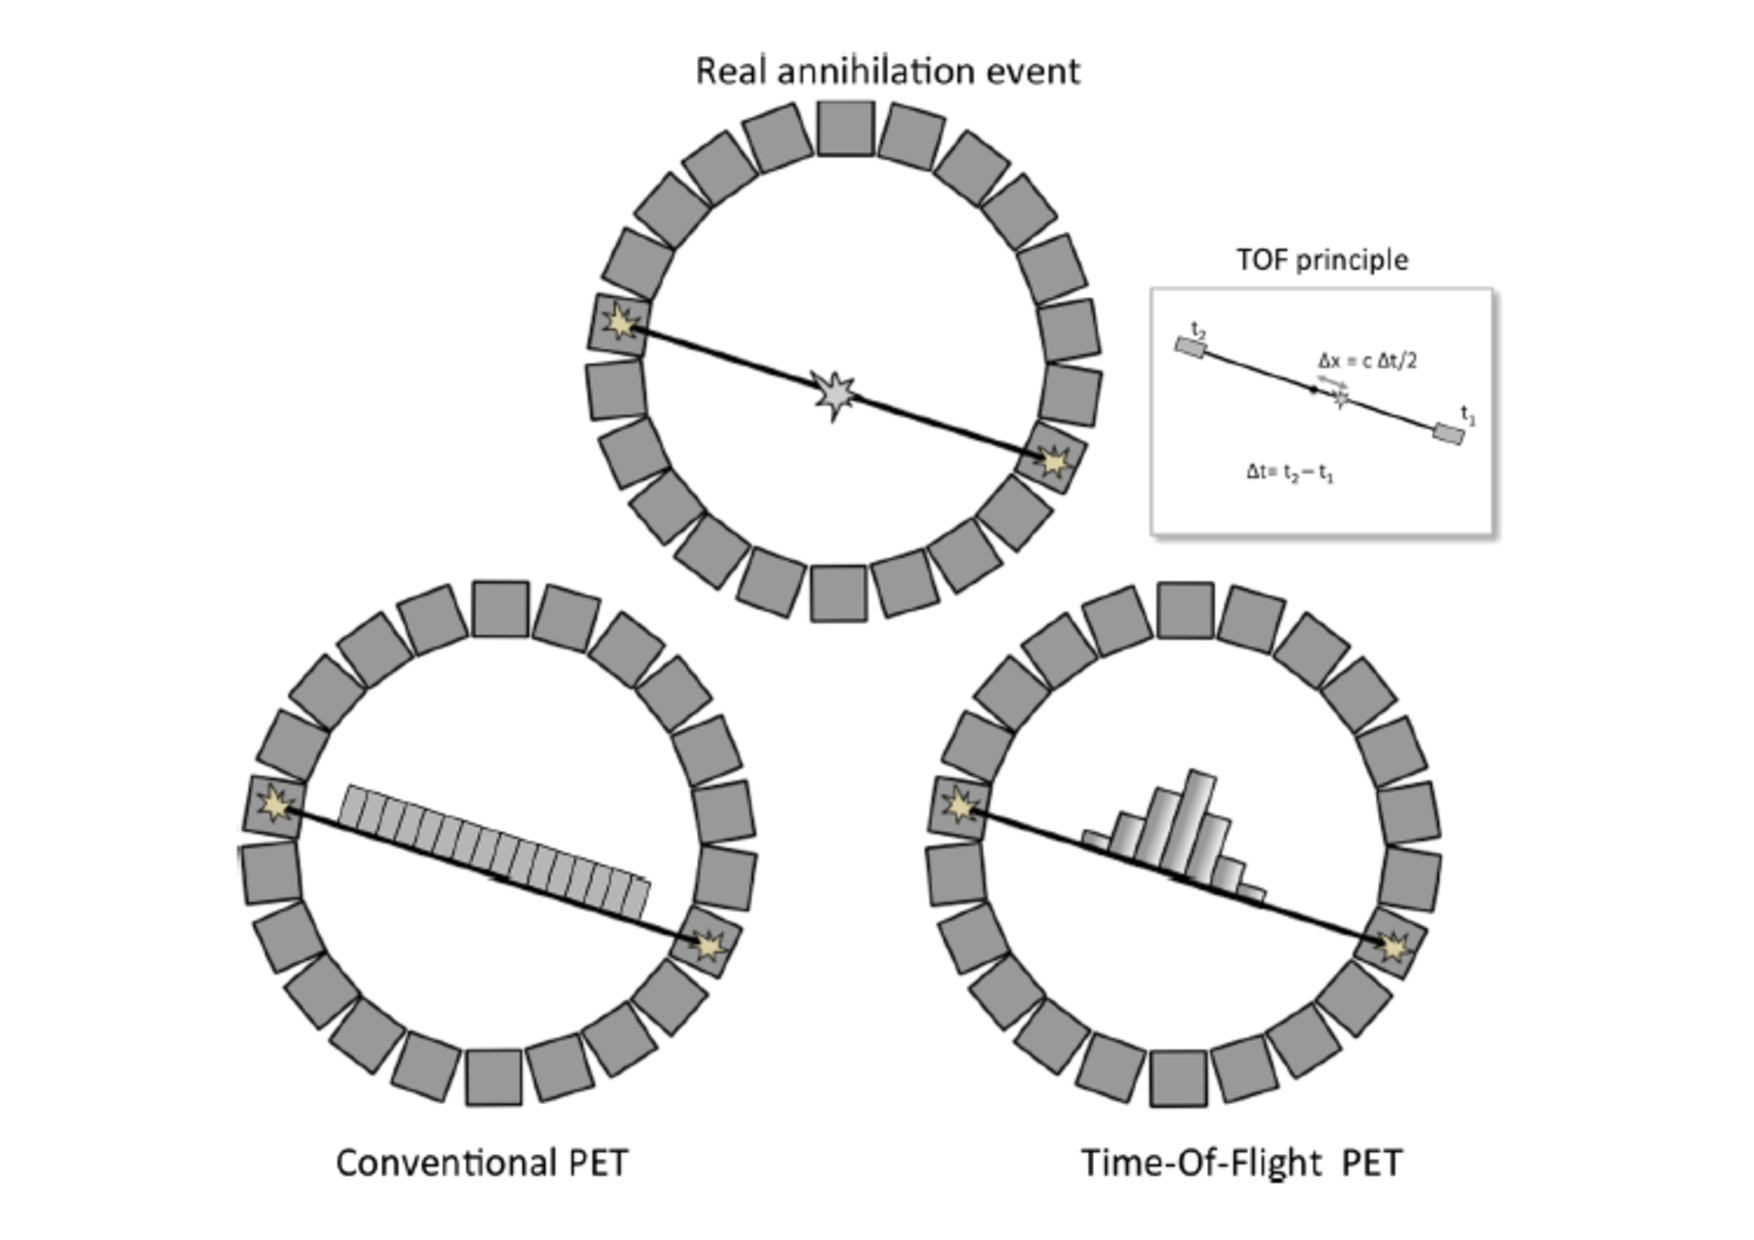
\includegraphics[width=0.8\textwidth]{03_GraphicFiles/chapter1_Introduction/PET_concept.pdf}
%\caption{Schematic representation of the \gls{pet} technique principle. In the top figure, a standard real annihilation event is presented, while in the bottom line the principle of conventional and \gls{tof}-\gls{pet} are compared. In~\cite{Vandenberghe2016}.}
%\label{chap1::fig::PETconcept}
%\end{figure}   
%
%\figurename~\ref{chap1::fig::PETconcept} (top) shows the concept of the \gls{pet} detection technque. The emitted positrons annihilate with human tissue electrons after traveling few mm distances, and 511~keV back-to-back photons are produced and can be detected in coincidence with \gls{pet} machines. The spatial distribution of the $\beta^+$ decay points can be then obtained via the reconstruction of the so-called \enquote{lines of response} connecting the two detected photons, and it correlates, even if not directly, to the dose profile. \figurename~\ref{chap1::fig::PETrangeProf} shows the one-dimensional $\beta^+$ activity profiles along the beam axis for various incident beam types impinging on a \gls{pmma} target. The positron emitter distribution dependence on the beam nature clearly emerges from these profiles, but a form of indirect correlation with the dose profile distal edge is always verified. In particular, a remarkable difference exists between light ions (protons, $^3$He and $^7$Li), for which the induced activity is almost only due to target residuals, and heavier ones ($^{12}$C and $^{16}$O), with a considerable contribution also coming from projectile fragmentation sub-products, which concentrate near the end of the range, explaining the activity peak. The investigation of the correlation between delivered dose and $\beta^+$ detected activity must face several issues, as highlighted in~\cite{Parodi2004}, mainly connected to the difficulty to retrieve quantitative information from \gls{pet} images and to wash-out effects. Long-lived positron emitters, indeed, can be transported away from the production point by blood flow and metabolic processes, affecting the precision of the obtained images. This effect has been deeply studied experimentally at \gls{himac} with rabbit tissues and Anger-type scintillation cameras~\parencite{Mizuno2003, Tomitani2003}, and, more recently, at \gls{gsi} with $^{12}$C beams~\parencite{Fiedler2008}. A reduction of a factor up to 1.5 in the precision of the range determination due to wash-out processes is reported, and a correlation between biological half-life and local dose has been verified and used in simulation to improve the quality of \gls{pet} images. Although several research efforts have been dedicated to improve the precision of the dose recovery from $\beta^+$-emitter distributions~\parencite{Parodi2006, Parodi2007, Parodi2010}, the only feasible solution for the monitoring of dose delivery is the comparison of measured distributions to simulated ones~\parencite{Ponish2004}. These Monte Carlo simulations are based on the planning \gls{ct} scan, the irradiation scheme, the detector geometry, the imaging procedure; deviations in the delivered dose caused by patient positioning or anatomical modifications can be detected, mainly because they are reflected in changes in the maximum particle range in the target tissues. Thus, the main quality criterion of the \gls{pet} monitoring method is the precision in the measurement of range shifts with respect to the predicted ones~\parencite{Fiedler2010}. The accuracy of the reference simulated activity distribution has advanced in the last years, but it is still limited by the lack of underlying cross-sectional data, the not perfect knowledge of the elemental composition of the patient and the complex prediction of metabolic wash-out processes. Complementary imaging modalities can give fundamental contributions to the simulation predictions: for example, the use of supplemental \gls{mri} data has been proposed to better analyze local wash-out effects. In addition to this, the implementation of hybrid \gls{pet}-\gls{ct} systems, preferably with dual-energy \gls{ct}, would improve the conversion of \gls{ct} information to the material composition needed for the \gls{pet} simulations~\parencite{Landry2013}.  
%
%\begin{figure}[!htbp]
%\centering
%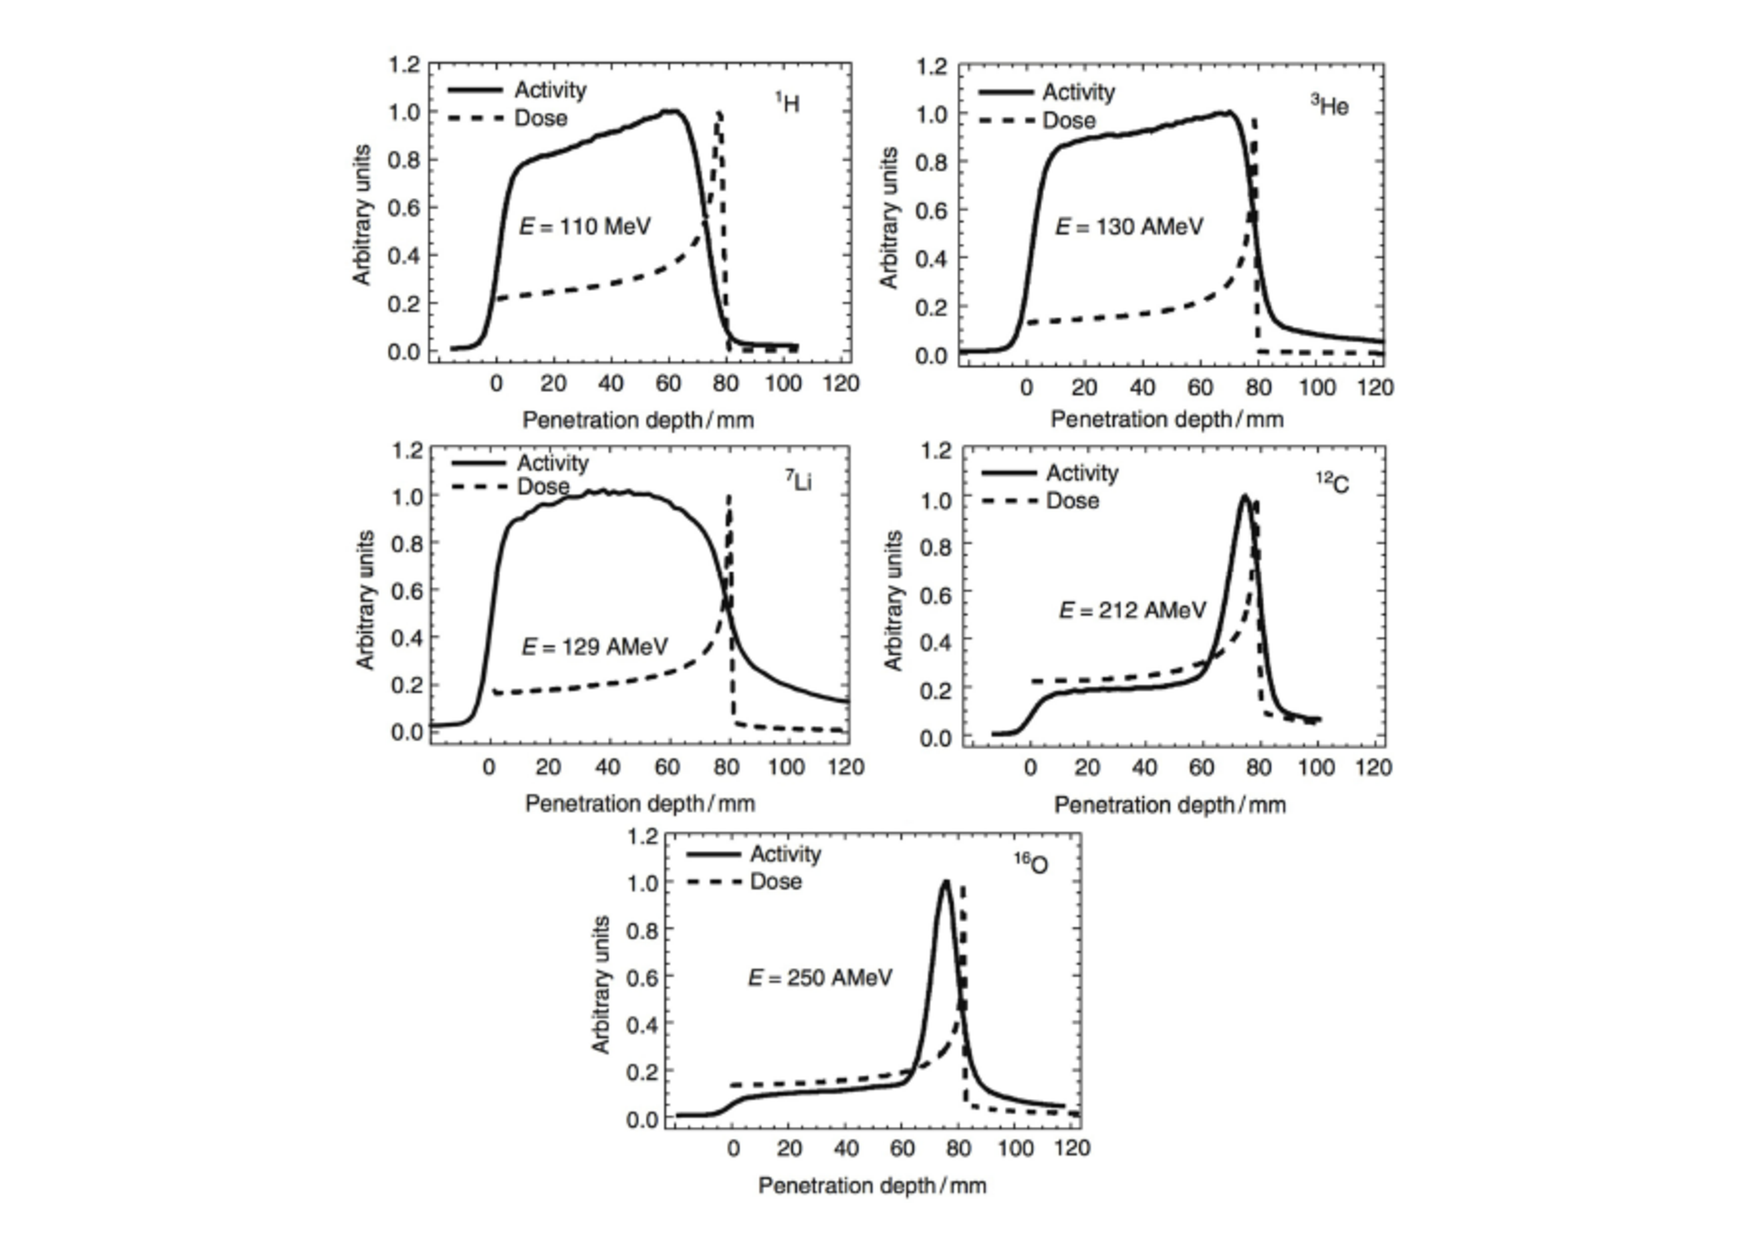
\includegraphics[width=0.98\textwidth]{03_GraphicFiles/chapter1_Introduction/PETrangeProf.pdf}
%\caption{$\beta^+$ activity profiles for various ion beams impinging on a \gls{pmma} thick target. The depth-dose profiles are also shown in dashed lines for comparison. In~\cite{Fiedler2012}.}
%\label{chap1::fig::PETrangeProf}
%\end{figure}   
%
%The \gls{pet} data acquisition can be performed following three main strategies:
%\begin{itemize}
%\item In-beam data acquisition: the \gls{pet} system is integrated in the beam delivery system and the data acquisition is performed during or immediately after irradiation in the treatment room. In synchrotron facilities, a further solution is represented by acquisitions in the time between different spills, while for cyclotrons data-taking during beam extraction has been explored and seems feasible~\parencite{Kraan2014}. On one hand, this method is advantageous because it allows detecting short-lived isotopes, thus increasing the available statistics, and reducing the effects of biological processes. Moreover, the patient position does not change with respect to the treatment. On the other hand, the integration of \gls{pet} scanners in the treatment site can be costly and cause limitations on the detector geometry affecting detection efficiency and, consequently, image quality. The scanner should not be directly exposed to the beam in order to avoid damage and activation of active modules and electronics, and at the same time it should allow enough degrees of freedom for the patient table. The need of an opening for the beam portal typically results in the choice of planar dual-head configurations.
%\item In-room data acquisition: the installation of commercial full-ring \gls{pet} scanners in the treatment room, but not directly on the beam line, allows the so-called \enquote{in-room} data acquisitions quickly after the end of the treatment irradiation. This solution leads to longer treatment room occupation, because some minutes of imaging time is required to gain enough statistics, but allows one to use commercial machines, less expensive and more efficient than custom integrated scanners designed for in-beam applications. Moreover, patient positioning issues are minimized by the limited movements and signal wash-out is reduced.
%\item Off-line data acquisition: if the patient has to be transported out of the treatment room for the \gls{pet} scan, the implemented strategy is classified as \enquote{off-line}. The limited cost and treatment occupation time are probably the only advantages of this method, which suffers from relevant signal decay and wash-out processes given the long time between the end of the irradiation and the beginning of the \gls{pet} scan. Off-line images predominantly show activity from isotopes whose half-life is comparable or longer then the transportation and setup time, thus it is mainly restricted to $^{11}$C (half-life longer than 20 minutes), produced in relative small amount in proton therapy, more abundant in carbon treatments. The reduced number of available decays requires longer acquisition time with respect to in-beam and in-room solutions, which further enhance the effect of metabolic processes. The patient repositioning issues also contribute to the image quality degradation. 
%\end{itemize}
%A schematic view of the three \gls{pet} acquisition modalities is presented in \figurename~\ref{chap1::fig::PETmodes}. As mentioned in the three data acquisition modality description, the counting statistics is one of the fundamental parameters to be studied for the design of \gls{pet} monitoring solutions. It can be estimated as the integral of the decay curve shown in \figurename~\ref{chap1::fig::PETactDistr}, where the time intervals corresponding to the three acquisition strategies are separated. The curve is based on measurements performed at \gls{gsi} during therapeutic irradiation with carbon ions; an in-beam solution has been adopted, with 40~s additional data taking time after the irradiation. The in-room selected window lasts 3 minutes, and for the off-line case, long-time measurements of one patient have been used~\parencite{Fiedler2008b}. If 100\% is assigned to the number of registered true events in the in-beam condition, 50\% is estimated for the in-room solution and 58\% for the off-line data taking~\parencite{Shakirin2011}. It is then clear that off-line solutions are severely challenged by the extremely low signal, considerably lower with respect to the standard application of the employed commercial scanners (down to average activity values of few tens of Bq/ml~\parencite{Bauer2013}).
%The scanner geometry is another fundamental parameter to be considered: as mentioned, the chosen data-acquisition strategy determines the scanner design. In-room and off-line solutions can make use of commercial full-ring systems, with a complete field of view. In addition to this, modern combined \gls{pet}-\gls{ct} scanners enable an accurate co-registration of treatment and imaging position, so that the unavoidable patient movement due to transportation and repositioning can be partially corrected. The geometrical constraints imposed by in-beam integrated solutions cause reduced efficiency and restricted field-of-view, which are reflected in image artifacts~\parencite{Crespo2006}, particularly significant in the imaging of large tumor objects. Improvement can be provided by \gls{tof}-\gls{pet} detectors~\parencite{Crespo2007, Surti2011}, as discussed below.
%In~\cite{Parodi2015} the author highlights how the first historical attempts to implement \gls{pet} particle therapy monitoring, described in the following, have not relied on optimized instrumentation for the peculiar application. Anyway, the promising results obtained by several groups encouraged dedicated investigations which are leading to substantial improvements of such a technique in the last years. In particular, the application of gamma detectors with depth-of-interaction capability, also studied for standard diagnostics applications, has demonstrated its effectiveness in correcting parallax artifacts in the reconstructed images; improvements in data acquisition and synchronization with the accelerator radio-frequency offer the possibility of including the signal detected during the beam-on time for in-beam solutions, thus increasing the counting statistics and reducing the acquisition time; new adapted geometries, such as the Japanese OpenPET system~\parencite{Tashima2012, Yamaya2008}, recently finalized in its upgraded version~\parencite{Yamaya2017}, offer higher-efficiency alternatives to standard dual-head systems. 
%It is worth to dedicate particular attention to the already mentioned \gls{tof}-\gls{pet}, deeply studied in the last years, which already demonstrated improved imaging capabilities with respect to standard scanners. The measurement of the detection time of each of the two photons helps, through the calculation of the arrival time difference, in restricting the emission point along the reconstructed line of response and thus also in rejecting part of accidentals. In standard \gls{pet}, the three-dimensional reconstruction relies on the superposition of several lines of response and on filtered back-projection algorithms. The time information adds a second dimension to the line of response reconstruction, with the localization of the interaction point in a few cm along the line, depending on the detector time resolution. For example, a coincidence timing resolution of 600 ps \gls{fwhm} translates to a position uncertainty of 9 cm \gls{fwhm}. In~\figurename~\ref{chap1::fig::PETconcept} (bottom line), the \gls{tof}-\gls{pet} principle is sketched and compared to the conventional \gls{pet} detection scheme. 
%The potential benefits of \gls{tof} information in \gls{pet} image reconstruction were already understood since the early stage of its development for diagnosis purpose, and the first \gls{tof}-\gls{pet} systems were built already in the 1980s in the US~\parencite{Gariod1982}. They were based on \gls{csf} or \gls{baf2} scintillators, the best available at the time in terms of time resolution, but their spatial performance and sensitivity were poor with respect to conventional \gls{pet} scanners. The improvements in scintillating material as well as in \gls{pm} performance and reliability allowed for the first commercial proposal of a \gls{tof}-\gls{pet} scanner only in 2006, by Philips~\parencite{Surti2007}. The development of \gls{tof}-\gls{pet} machines is strongly connected to their application in diagnosis, and further details will be given in section~\ref{chap1::subsec::PET_NM}. As for particle therapy monitoring application, the \gls{tof} technique applied to \gls{pet} can be used to partially reverse the effects caused by non-complete angles of in-beam data collection~\parencite{Crespo2006}, and in general to improve the image quality. Various groups are developing detector solutions for clinical implementation of such a technique; some of them have already been tested on beam with promising results. They will be described in more details in the following, after a brief historical overview of the \gls{pet} application in particle therapy quality assurance. 
%
%\begin{figure}[!htbp]
%\begin{subfigure}[t]{.49\textwidth}
%\centering
%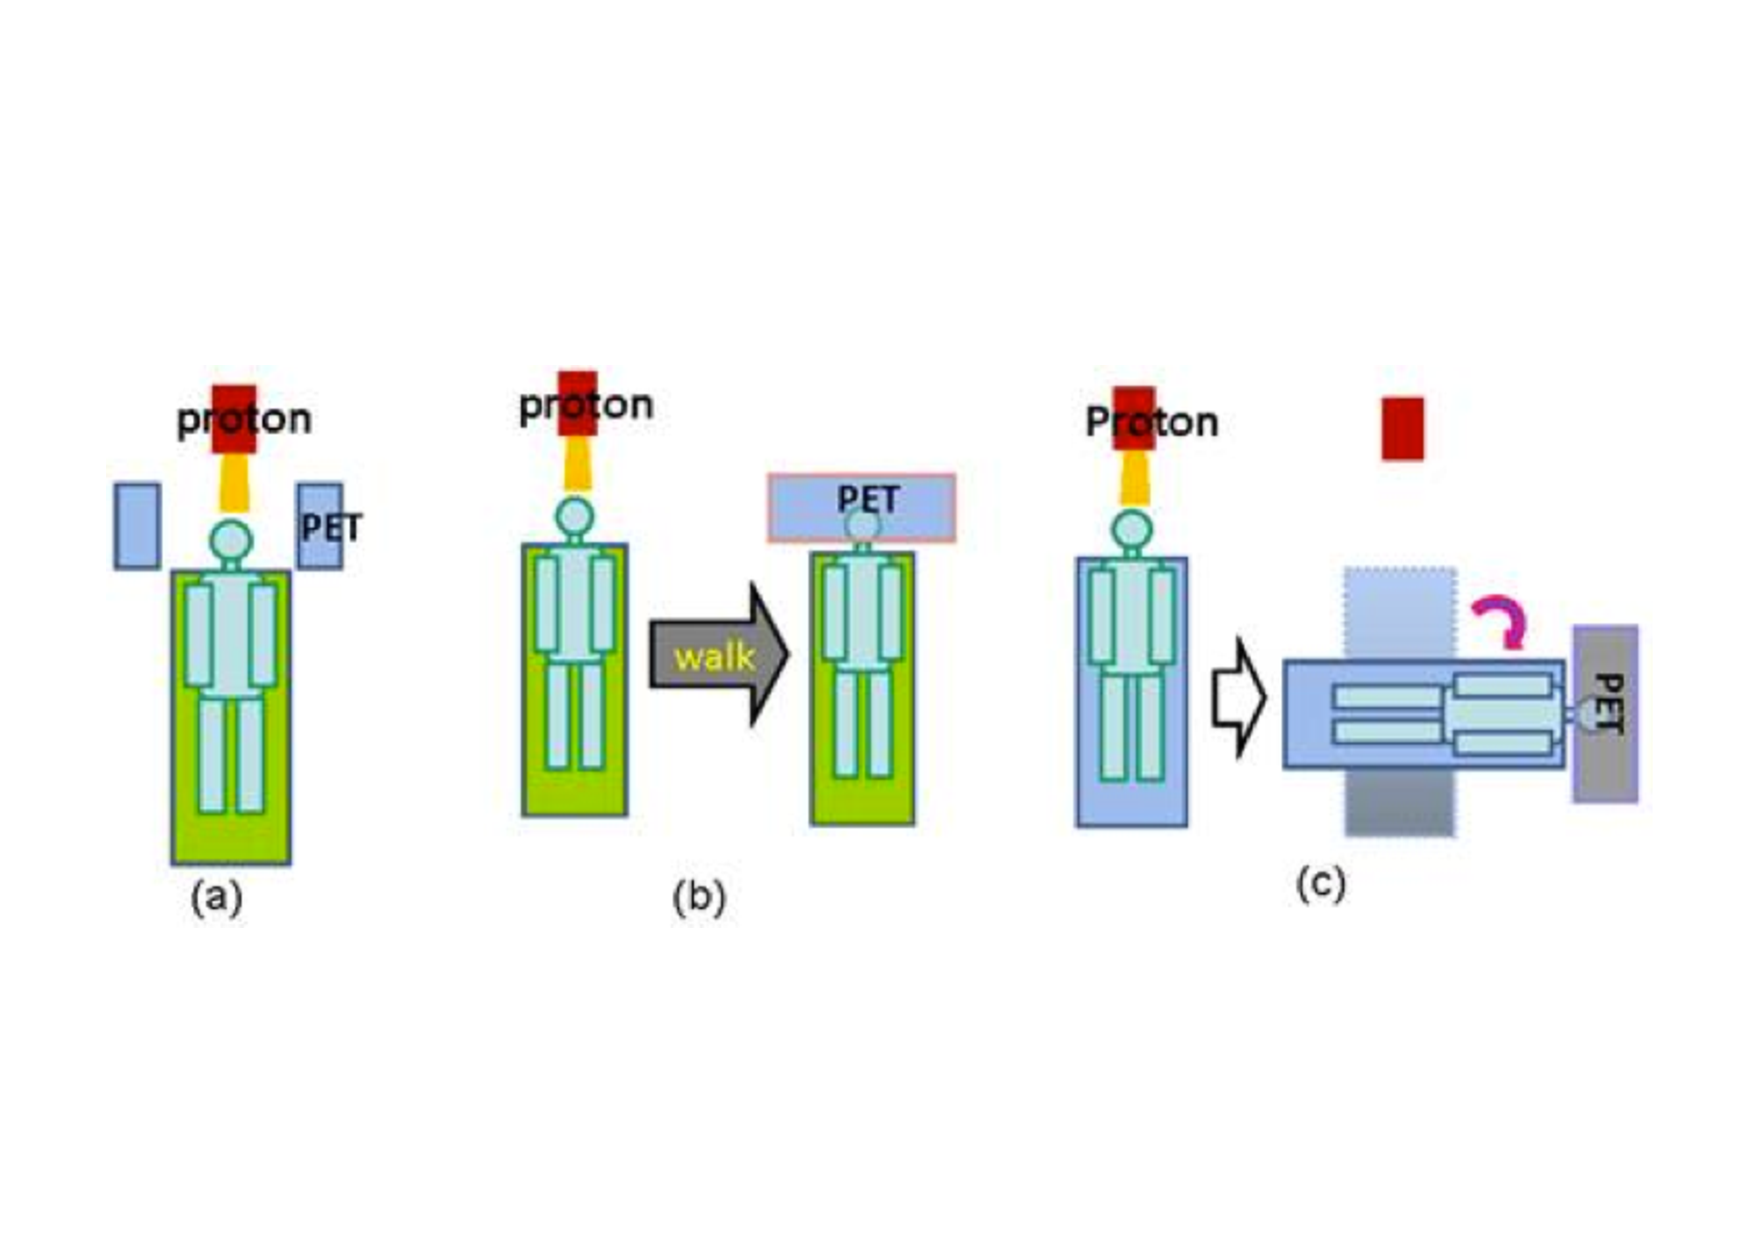
\includegraphics[width=0.98\linewidth]{03_GraphicFiles/chapter1_Introduction/PETmodes.pdf}
%\caption{Schematic view of the three \gls{pet} configurations for the application in ion range monitoring. Form left to right: in-beam, off-line and in-room \gls{pet}. In~\cite{Zhu2013}.}
%\label{chap1::fig::PETmodes}
%\end{subfigure}
%\begin{subfigure}[t]{.49\textwidth}
%\centering
%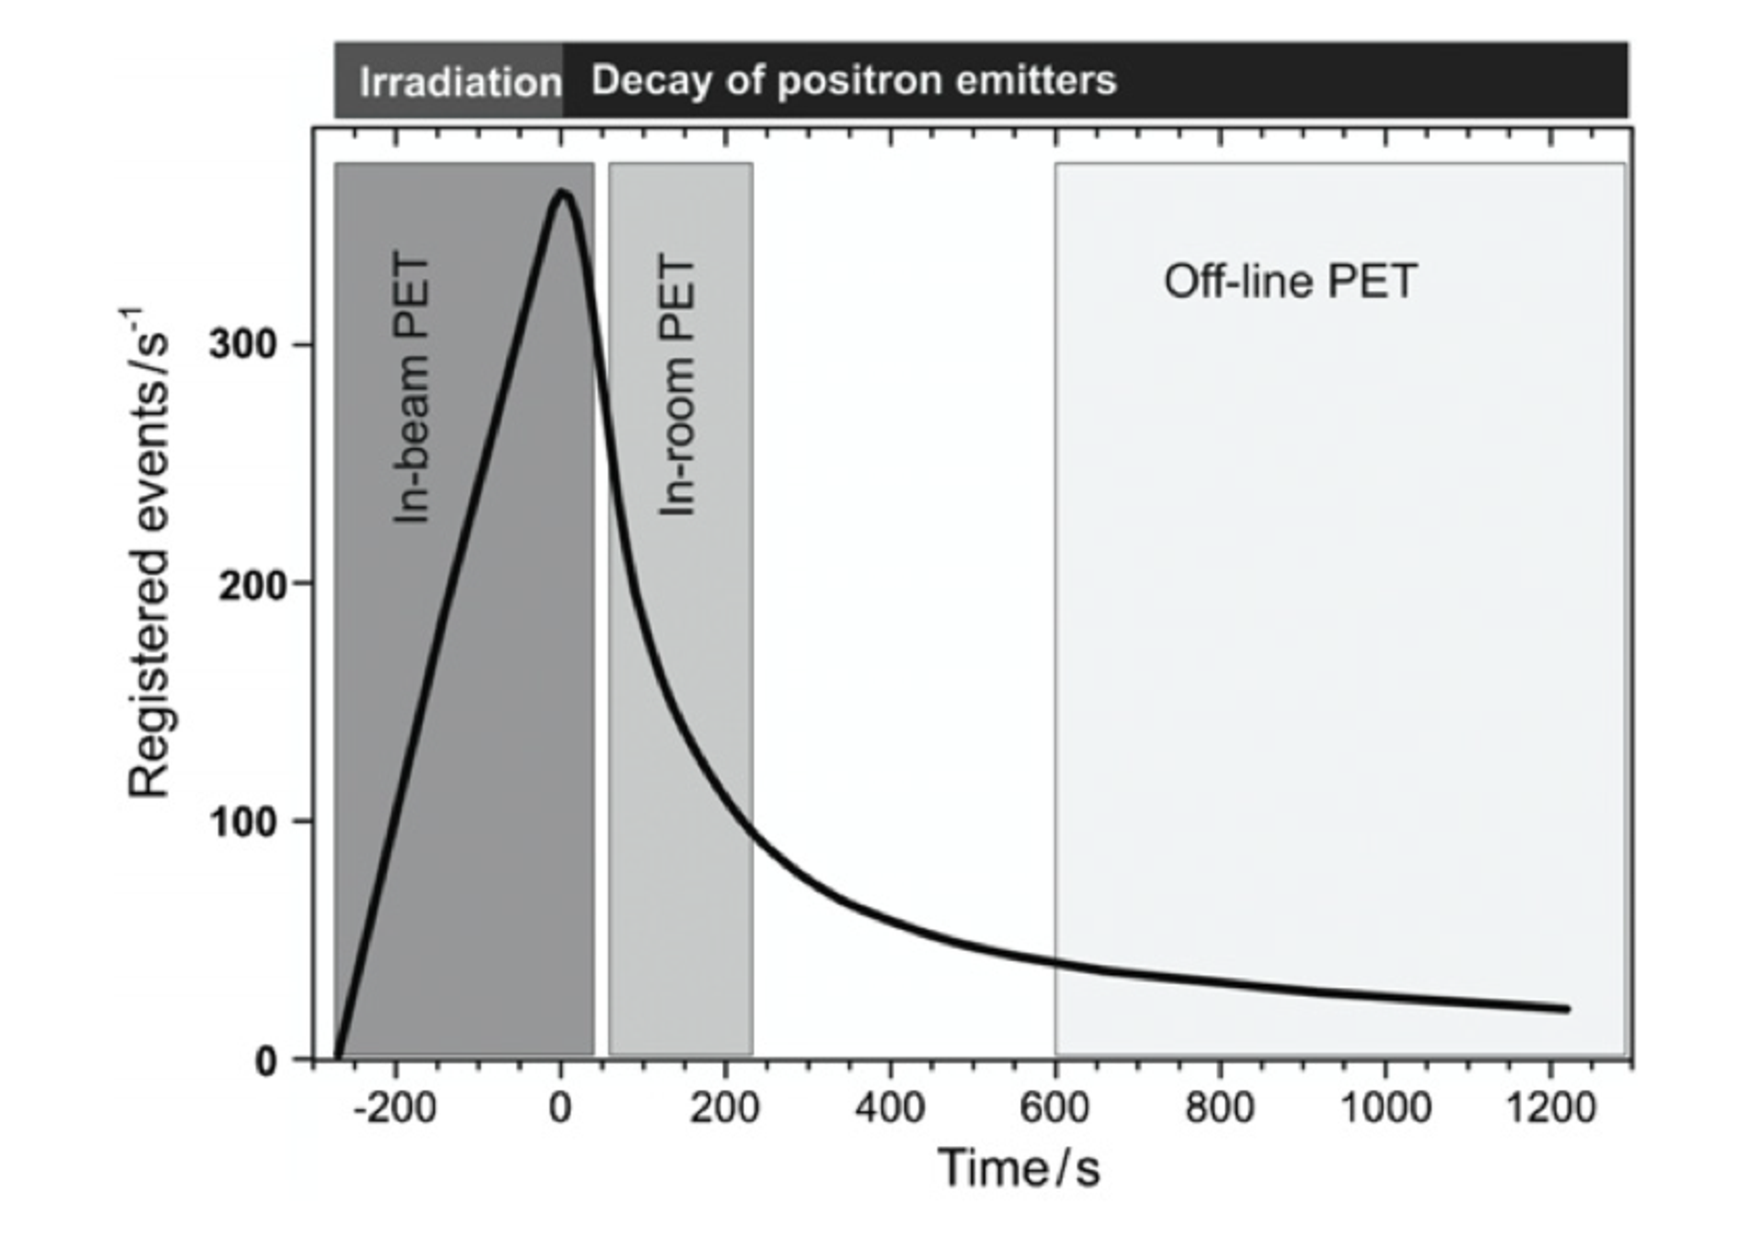
\includegraphics[width=0.92\linewidth]{03_GraphicFiles/chapter1_Introduction/PETactDistr.pdf}
%\caption{\gls{pet} registered events as a function of time corresponding to the measurement of one field during
%irradiation and up to 20 minutes after irradiation. The time intervals corresponding to  in-beam, in-room, and off-line \gls{pet} measurements are highlighted. In~\cite{Shakirin2011}.}
%\label{chap1::fig::PETactDistr}
%\end{subfigure}
%\caption{The application of the \gls{pet} technique to the monitoring of ion range in particle therapy includes three possible modalities: in-beam, in-room and off-line \gls{pet}, represented in the scheme in (a). The amount of registered events depends on the created positron emitter half-life, and thus on the implemented modality, as shown by the histogram in (b).}
%\label{chap1::fig::PETmodalities}
%\end{figure} 
%
%As emerges from the above paragraphs, \gls{pet} is probably the most extensively studied technique for online beam range verification and is at present the only method clinically implemented~\parencite{Enghardt2004}. The first published proposal of using \gls{pet} for range verification in particle therapy dates back to 1975~\parencite{Bennett1975}. In the next years, further suggestions were connected to pion~\parencite{Goodman1986, Shirato1989} and neutron therapy~\parencite{Vynckier1989}, but the actual clinical implementation was pioneered in the context of heavy ion therapy at \gls{lbl}~\parencite{Llacer1979, Chatterjee1981}. The original idea was to verify the correctness of $^{20}$Ne ion therapy treatment plans by delivering a low dose $\beta^+$ emitting ion beam (e.g. $^{19}$Ne) prior to the treatment and measuring its range via \gls{pet} imaging of the emitted photons; before the regular treatment with stable beams. Pilot experiments were conducted with a planar \gls{pet} camera based on two blocks of \gls{bgo} crystals, including measurements in a live dog~\parencite{Llacer1984b}. The experimental data showed interesting results, even if the use of a passive beam shaping system determined a significant activation of the \gls{bgo} camera (mainly due to neutrons) and, thus, a substantial noise level. Analog investigations using radioactive ion beams ($^{15}$O, $^{17}$F, $^{19}$Ne) were carried out in the nineties at \gls{gsi} with various \gls{pet} cameras~\parencite{Pawelke1996}, and further developments of this technique were obtained at the \gls{himac} facility~\parencite{Iseki2004, Kitagawa2006}, where a dedicated line was set up for radioactive beam based treatments~\parencite{Urakabe2001, Kanazawa2002}. The \enquote{autoactivation} process~\parencite{Tobias1971} described above (i.e. the production of radioactive nuclei in the target by incident beam of stable ions) makes anyway possible the implementation of \gls{pet} monitoring techniques on standard high-energy beams, and the first clinical implementation of such  technique was launched at \gls{gsi} in 1997, after the tests with radioactive beams mentioned above and fragmentation studies conducted with $^{12}$C, $^{16}$O, $^{20}$Ne beams on a \gls{pmma} target~\parencite{Enghardt1992}. An in-beam \gls{pet} system was designed and installed into the treatment room and has been employed routinely for monitoring the irradiation of more than 440 patients (mainly suffering from head-and-neck cancer), with data acquisitions performed in the pause of pulsed beam delivery. This experience proved how \gls{pet} is a valuable tool for particle therapy quality assurance~\parencite{Enghardt2004}. In parallel to these developments in Germany, an off-line solution was implemented at \gls{nirs} with a commercial full-ring volumetric scanner, but it was not used in clinics. As previously explained, notwithstanding the lacking peak structure in the activity profile (cf. \figurename~\ref{chap1::fig::PETrangeProf}), also proton irradiation therapy can be monitored by \gls{pet} scanners. Various detailed studies investigated its feasibility and performance in the nineties~\parencite{Litzenberg1992, Paans1993, Oelfke1996, Litzenberg1999}. Two groups worked in parallel on clinical studies of \gls{pet} monitoring in proton therapy. In Japan, a dual-head \gls{pet} scanner has been installed at the National Cancer Center, Kashiwa~\parencite{Nishio2006}: it is based on high-resolution \gls{bgo} detector components and integrated in the proton gantry. The measurements are collected immediately after irradiation (in-room solution), mainly due to the considerable radiation background during the continuous beam delivery and the passive beam shaping. The satisfactory results led to the implementation of a daily \gls{pet} workflow, which allowed the research group to follow the anatomical changes of the patient during the treatment progress and correct the treatment planning. The test of this method included 48 patients suffering from head-and-neck, liver, lung, prostate and brain tumors~\parencite{Nishio2010}. In the US, at the \gls{mgh}, Boston, a pilot clinical study was performed with an off-line solution which made use of a commercial full-ring scanner~\parencite{Parodi2007}. The \gls{pet} scan was performed about 20 minutes after proton irradiation. The off-line approach has been deeply studied in the same context in those years, and compared to in-beam \gls{pet} solutions in cyclotron and synchrotron based scenarios~\parencite{Parodi2008, Knopf2011}. The advantage in terms of available statistics for in-beam solutions has been measured: the ratios between the amount of physical decays available for in-beam and off-line detection range from 40\% to 60\% for cyclotron-based facilities, to 65\% to 110\% (carbon ions) and 94\% to 166\% (protons) at synchrotron-based facilities~\parencite{Parodi2008}. The in-room solution has also been explored at the same institution, with an acquisition time reduced to less than 5 minutes thanks to the higher sensitivity with respect to the off-line modality~\parencite{Zhu2011}.  
%At \gls{hit}, in Germany, both an in-beam~\parencite{Sommerer2009}, and an off-line solution~\parencite{Bauer2013} have been tested, while alternative off-line solutions have been implemented in Japan~\parencite{Hishikawa2002} and US~\parencite{Hsi2009}. 
%With the aim of extending the field of view and thus enhancing the sensitivity of in-beam \gls{pet} designs, Japanese researchers proposed the already mentioned OpenPET as a new geometrical solution. Its first-generation prototype is composed of two complete rings, with the beam port between the two~\parencite{Yamaya2008, Yamaya2009} and the possible implementation of an integrated \gls{ct}. A more efficient geometry has been proposed some years later, consisting of a single-ring which can provide an accessible and observable open space with higher sensitivity and reduced number of detectors compared to the previous generation one~\parencite{Tashima2012}. The ring is cut at a slant angle in order to be disposed at a certain angle with respect to the beam line, but maintain parallel detector modules orientation. A similar solution was proposed in~\cite{Crespo2006}, but with a conventional \gls{pet} ring with an oblique orientation with respect to the beam direction (\enquote{slant \gls{pet}}). A small prototype of single-ring OpenPET was produced, consisting of 4 layers (16$\times$16 array) of Zr-doped GSO scintillators with a size of 2.8$\times$2.8$\times$7.5~mm$^3$ read out by H8500 Hamamatsu \glspl{pm}~\parencite{Tashima2016}, and tested at \gls{himac} with radioactive $^{11}$C beam. The prototype can operate in open and closed mode, the second only adapted for acquisition in beam-off condition, and easily arranged in the two configurations. The tests, performed in the two modes, the spatial resolution and sensitivity were 2.6~mm and 5.1\% for the open mode and 2.1~mm and 7.3\% for the closed one. A rapid transformation to a closed arrangement is foreseen by the authors immediately after irradiation in order to minimize the decrease of resolution and sensitivity. After these encouraging results, a full-size whole-body  version of the single-ring OpenPET has been recently completed~\parencite{Yamaya2017}.    
%Extensive studies about \gls{pet} monitoring have been and are being carried out also in Italy. An in-beam prototype consisting of two planar heads made of \gls{lyso} crystals~\parencite{Vecchio2007}, 5$\times$5~cm$^2$ active area, has been tested at the proton therapy center CATANA, in Catania, equipped with a 62~MeV beam line for ocular tumor treatments~\parencite{Cirrone2003}. The measurements validated the detector design~\parencite{Attanasi2008}, which has been called DoPET and also compared to the in-beam system installed at \gls{gsi} with simultaneous measurements of $\beta^+$ activity induced in a \gls{pmma} target~\parencite{Attanasi2009}, showing improved spatial resolution mainly due to the smaller crystals. The field of view of the first prototype was a major issue, so that an extended version with 10$\times$10~cm$^2$ active area per head has been realized and tested by the Italian collaboration at \gls{cnao}~\parencite{Rosso2013, Kraan2015} and in Catania~\parencite{Sportelli2014, Camarlinghi2014}. The comparison of the results with Monte Carlo simulated data showed good agreement; for treatment-like data taking, the ability of the system to give valuable feedback on particle range on homogeneous targets within 2~minutes after irradiation has been demonstrated, but the data collected during beam-on time were not satisfactory.
%In the context of \gls{pet} data taking during beam-on time, several studies have been performed concerning short-lived isotopes, which has to be included in the total activity evalutation in case of in-spill acquisitions. Already mentioned in the DoPET related publications, they have been deeply studied experimentally. Defined as positron emitters with half-life below 19~s, the ones significant for in-vivo \gls{pet} monitoring have been identified in~\cite{Dendooven2015}: in particular, the author concludes that the contribution to the $\beta^+$ activity given by $^{12}$N isotopes in the first tens of seconds after irradiation can potentially lead to real-time range verification of proton therapy with the implementation of optimized knife-edge detectors, providing equal or superior information with respect to \gls{pg} detection (see section~\ref{chap1::subsec::PGgeneral} and chapter~\ref{chap::2}). A proof-of-principle experiment for the detection of such isotopes has been performed at the KVI-CART cyclotron with 90~MeV protons and a \gls{pet} system based on \gls{lyso} crystals coupled to  digital \glspl{sipm}~\parencite{Buitenhuis2017}.  A range shift of 5~mm could be measured with 3~mm accuracy using the $^{12}$N activity profile. 
%Another \gls{pet} prototype based on \glspl{sipm} is the one developed by the Italian \gls{inside} collaboration~\parencite{Marafini2015}, and described in~\parencite{Bisogni2017}. The design is based on fast pixelated \gls{lfs} scintillators coupled one-to-one to \glspl{sipm}. The readout electronics has been developed to accept the count rate expected from synchrotron beams during the spill phase~\parencite{Rolo2013}. The whole system also includes a charged particle tracker (\enquote{dose profiler}), and its design has been studied for the installation on the \gls{cnao} beam line, where it has been tested and is at present in operation. The first characterization tests performed with \gls{pmma} and anthropomorphic phantoms demonstrated the capability of the system to operate in both beam-on and -off condition, and the comparison between in-spill and interspill data showed a substantial agreement in terms of distal fall-off. The results were also in agreement with Monte Carlo simulated data. In December 2016, the \gls{inside} \gls{pet} was also tested during a patient treatment, and the possibility of online monitoring of proton therapy in clinical conditions has been demonstrated~\parencite{Ferrero2018}. For carbon ion irradiation, in-spill measurments have not been satisfactory due to the large amount of random coincidences, but at treatment end, or at most 20 s afterwards, the range measurement has been verified to be reliable within 1–2 mm, when comparing both different experimental sessions and data with simulations~\parencite{Pennazio2018}. 
%Digital photon counters have been the basis for the development of \gls{tof}-\gls{pet} prototypes, attractive solution for improved spatial reconstruction capabilities in both full-ring and dual head solutions. Within the European project ENVISION, two different configurations have been explored for in-beam \gls{tof}-\gls{pet} imaging: one of them relies on \gls{lyso} crystal read out by \gls{sipm}, and a \gls{tof} resolution of 235~ps \gls{crt} \gls{fwhm} have been obtained~\parencite{Morrocchi2012}. The alternative solution involved low-cost gas detectors (multigap \gls{rpc}), but it was less performing in terms of time resolution~\parencite{Watts2013}. Another small prototype based on \gls{lyso} crystal and digital photo-sensors, presented in~\parencite{Degenhardt2012}, has been tested for \gls{tof} application in clinical conditions at \gls{hit} with protons. The acquisitions were performed in the pauses between spills or after irradiation, providing relevant information for a future development of a clinical size detector~\parencite{CambraiaLopes2016}.    
%
%The \gls{clarys} collaboration, in France, also included in its research project proposal the development of an in-beam \gls{pet} detector; the advancement of the study is at present limited to the \gls{lpc} research group. The prototype, called \gls{dpga} (French) or \gls{lapd} (English), is composed of 240 identical 13$\times$1$\times$315~mm$^3$ \gls{lyso} crystals glued to \glspl{pm}, assembled in groups of four (\enquote{quartets}) with similar gain \glspl{pm} for the read-out on a custom \gls{fe} board~\parencite{Montarou2016}. The system has been first tested in a hospital in Clermon-Ferrand with a \gls{pmma} phantom and \gls{fdg} injected radiotracer (some tenth of MBq of activity), and then with proton beams at \gls{hit}, in a reduced-size version. These first tests have been used to validate and characterize the detector, but limited acquisition rate capabilities have been verified with the preliminary \gls{vme}-based solution. The prototype is now installed at the \gls{cal} in Nice, on the 65~MeV line, and the new acquisition system based on \gls{utca} is at the test stage.  
%
%\gls{pet} is at present the only applied solution for ion range monitoring in clinical conditions~\parencite{Enghardt2004}, and, as described, the research is ongoing to provide real-time control capabilities with improved image quality. Its principle can also be applied to hybrid systems, investigated in the last years and briefly mentioned in section~\ref{chap1::subsec::rangeComplTechniques}, including the detection of $\beta^+$ activity in combination with \glspl{pg} (see section~\ref{chap1::subsec::PGgeneral} and chapter~\ref{chap::2}) or additional single photon emission. This implementation will probably imply compromises in the individual technique performance, but their complementary information can open new perspectives for in vivo ion range verification.   

\subsubsection{Prompt-gamma detection}\label{chap1::subsec::PGgeneral}
An alternative way to access valuable information about the Bragg peak position of both proton and carbon ion beams in human tissue is represented by the detection of high-energy photons promptly emitted as a by-product of nuclear interactions (see section~\ref{chap1::subsec::Physics}). For many years, this kind of radiation was investigated as a source of background in \gls{pet}-based monitoring system~\parencite{Parodi2005}, mainly because the produced photon energy is too high to be detected with standard devices like \gls{spect} cameras~\parencite{Kraan2015b}. The idea of using prompt-gamma radiation to obtain a direct and instantaneous verification of the beam stopping position in tissues was first proposed by Stichelbaut and Jongen at the \nth{39} \gls{ptcog} meeting in 2003~\parencite{Stichelbaut2003}. Experimental verification of the correlation between prompt-gamma profiles and Bragg peak position has been presented for protons and carbon ions~\parencite{Min2006, Testa2008} few years later, and the method is nowadays deeply studied as a promising solution for online range verification in clinical conditions. The research efforts involve imaging and time or energy resolved techniques, for which several detection solutions are being developed and tested. 
In section~\ref{chap2::sec::PGionRangeMonitoring} the prompt-gamma detection physical principle for range verification and the state of the art of this research field are presented. The details of the detection solution under development by the \gls{clarys} collaboration, within which this thesis has been conducted, are presented in chapter~\ref{chap::3} and chapter~\ref{chap::6} (dedicated to the detector beam tests); the simulation results of the clinical application of the Compton camera for proton and carbon ion range verification are illustrated and discussed in chapter~\ref{chap::4}.   

\subsubsection{Interaction Vertex Imaging}\label{chap1::subsec::IVI}

As described in section~\ref{chap1::subsubsec::particleCT}, high-energy traversing ion beams can be used for radiography and tomography purposes in order to increase the accuracy of stopping power measurements for treatment planning. The detection of protons can also be used as a treatment monitoring technique, if secondary protons produced in nuclear collisions are considered. This ion range control modality has been proposed less than a decade ago~\parencite{Dauvergne2009, Amaldi2010b} and is generally referred to as \gls{ivi}. The charged particles created during fragmentation processes in the target can be energetic enough to exit the patient and are most likely forward directed; thanks to a detector located downstream from the patient, their trajectories can be then reconstructed and extrapolated back to the production point. The principle is similar to vertex identification problems in fixed target particle physics experiments. The comparison of the obtained distribution with the one simulated at the treatment planning stage provides a means of controlling the ion range. In addition, the amount of emerging charged particles can be, in principle, correlated to the dose. Given the larger amount of protons generated by carbon irradiation with respect to proton ones~\parencite{Gunzert-Marx2008}, this method is more suitable for carbon ion therapy monitoring.  
A feasibility study has been presented in~\cite{Henriquet2012}; the authors investigated the possible implementation of such a control in carbon ion therapy with Geant4 simulations. The modeled detector is composed of two pairs of 50~\charmum thick pixelized \gls{cmos} trackers, placed at an angle of 30 degrees with respect to the beam direction, and two methods have been tested, one based on the coincidence of two protons emitted from the same vertex, the second relying on the incident carbon ion trajectory determined by a beam hodoscope in coincidence with single secondary proton detection. The study showed the possibility of achieving millimetric precision on the Bragg peak position in the ideal case of homogeneous targets with pencil beams of 2$\times$10$^5$ carbon ions. Experimental tests have been conducted at \gls{hit} with a similar setup involving hybrid-pixel detector with \gls{cmos} read-out, and with higher statistics the accuracy in the beam range monitoring was found to be 1-3~mm~\parencite{Gwosch2013}. In the experimental studies reported in~\cite{Agodi2012} and~\cite{Piersanti2014}, \gls{pmma} targets have been irradiated with mono-energetic carbon-ion beams at different energies, and secondary protons have been measured with systems placed at 60 and 90 degrees with respect to the beam direction; the results have been compared to FLUKA predictions, and reasonable agreement has been verified. The detector developed by the TERA Foundation at CERN~\parencite{BucciantonioPhD2015} has been also proposed as a solution for \gls{ivi}, but it has never been tested for this purpose. Recently, the method was tested in clinical conditions with measurements performed at \gls{hit}; the resolution of the Bragg peak position was found to be about 4-5~mm in an homogeneous \gls{pmma} phantom with 10$^6$ incident carbon ions and a tracker of 2$\times$2~cm$^{2}$~\parencite{Finck2017}.
The \gls{ivi} method could therefore monitor the Bragg peak position with a promising resolution in clinical conditions, but further efforts are needed to improve Monte Carlo predictions of the angular distribution of the fragments, as well as to increase acceptance and efficiency of the employed detectors. 

\subsubsection{Other techniques}\label{chap1::subsec::rangeComplTechniques}

The detection of secondary radiations emerging from the patient body during particle therapy is not the only available channel for measuring the ion stopping position and, more generally, verify the treatment delivery. The dose delivered in photon and electron treatments \myMarginnote{Point measurements} have been measured in vivo with diodes and thermo-luminescence dosimeters, as reviewed in~\cite{Essers1999}, and implantable devices with wireless readout have been introduced in standard radiotherapy~\parencite{Black2005, Scarantino2008} and investigated for proton range verification. The main challenge is the positioning of the detector, which strongly influences the measurement of the steep dose distal fall-off of ion beams, and two solutions have been proposed by the same author to overcome this issue. 
The residual range of the irradiation beam can be retrieved at each position via its time dependence, which is unique at every point in depth~\parencite{Lu2008}. This method, proposed for passively scattered beams but also applicable to actively scanned ones, has been tested with a small \gls{ic}, and sub-millimeter precision for the determination of the proton range at a specific position in water has been proven (even if in ideal conditions). The second proposed method relies on the delivery of a pair of complementary fields, with sloped depth dose profiles~\parencite{Lu2008b}.  The ratio between the two measured distributions can verify the radiological path length. As the previous one, this approach has been experimentally tested, in this case with a commercial implantable dosimeter~\parencite{Lu2010}, and dose ratios have been measured with a relative uncertainty of 1-3\%. Notwithstanding the valuable obtained results, the applicability of both solutions is strongly limited by the need of implanting devices in the patient, ideally close or within the tumor, which is often not possible. In any case, possible improvements are still being studied recently~\parencite{Toltz2017}.
An alternative way to measure the range with simple detectors in one dimension is the so-called \enquote{range probe}~\parencite{Mumot2010, Watts2009}. This concept relies on the direct measurement of the Bragg peak of single high-energy pencil beams passing through the patient, in a sort of simplified mono-dimensional version of proton radiography discussed in section~\ref{chap1::subsubsec::particleCT}, and can in principle both validate the range in vivo and verify patient positioning errors with low additional dose.        
\gls{mri} imaging has also been considered as a way to observe delivered dose distributions\myMarginnote{\gls{mri} imaging}. The application of such a technique is made possible by the changes induced by radiations in tissues, and it has been investigated mainly for spine patients~\parencite{Gensheimer2010}, but the accuracy was not sufficient to verify the ion range. However, the high spatial resolution achievable with commercial scanners is a good point in favor of further investigations. 
The improvement of ultrasound imaging techniques \myMarginnote{Acoustic imaging} determined in the last years a renewed interest on its application to ion range verification. It has been demonstrated that iono-acoustic detectable signals are produced by the localized dose deposition of ion beams~\parencite{Tada1991}, which induces local temperature increases and, thus, a pressure wave~\parencite{Parodi2015b}; these pulses have been already measured in 1995 in a proton therapy treatment~\parencite{Hayakawa1995}.  A schematic view of the detection principle is presented in \figurename~\ref{chap1::fig::ionoacoustic}. Recently, tests on proton beam have been performed at the \gls{cal}, in Nice, with mono-energetic beams in the energy range 145-227~MeV~\parencite{Lehrack2017}; as the author stated, the method as been been proven to be a cost-effective, fast and accurate way to obtain quality control measurements in proton therapy, with sub-millimeter range determination accuracy (the results have been compared to reference data collected with an \gls{ic}). However, it has been highlighted how the synchrocyclotron offered ideal condition for the application of iono-acoustic measurements, thanks to the delivered intense and short (microsecond) bunches. \gls{snr} is an additional problem at the present development stage, but it has to be pointed out that iono-acoustics offers a method not only to locate the Bragg peak, but also to correlate it with an ultrasound tumor image; the research effort is so clearly justified, and improvements are expected in the next years. To be noticed, anyway, that the iono-acoustics probes can be used only with soft tissues, so that their application, for example in head-and-neck treatment monitoring seems not feasible.
In addition to the deeply investigated techniques based \myMarginnote{Bremsstrahlung imaging} on secondary particles generated by nuclear reactions (\gls{pet} and \glspl{pg}), there are also bremsstrahlung photons coming from secondary electrons generated during ion deceleration. The basic principle is explained in~\cite{Yamaguchi2012}, where the author highlights that the dependence of the bremmstrahlung photon energy spectrum on the incident beam energy provides a method to control the beam range. In particular, secondary electron bremmstrahlung dominates at low ion energies, close to the Bragg peak, and its energy spectrum allows one to retrieve the correlated Bragg peak position. A complete experimental confirmation has been provided with measurements performed in Japan in different centers (\gls{himac} among them) with carbon ion beams and a \gls{cdte} detector, involving also background estimates. This technique provides in principle an overall better sensitivity with respect to \gls{pg} detection and \gls{pet}, and completely avoids the wash-out effects which affect positron emitter activity measurements, and has been developed in the last years. As secondary electron bremmstrahlung cross section scales as Z$^2$, this method is potentially advantageous for carbon ions. In particular, mono-energetic carbon ion beams have been recently imaged with a pinhole gamma camera~\parencite{Yamaguchi2018}, but the clinical necessary resolution in detecting range shifts has not been achieved yet. In addition, given the low energy of the emitted Bremsstrahlung photons, this technique is intrinsically limited to superficial tumor treatment control.

\begin{figure}[!htbp]
\begin{subfigure}[t]{.49\textwidth}
\centering
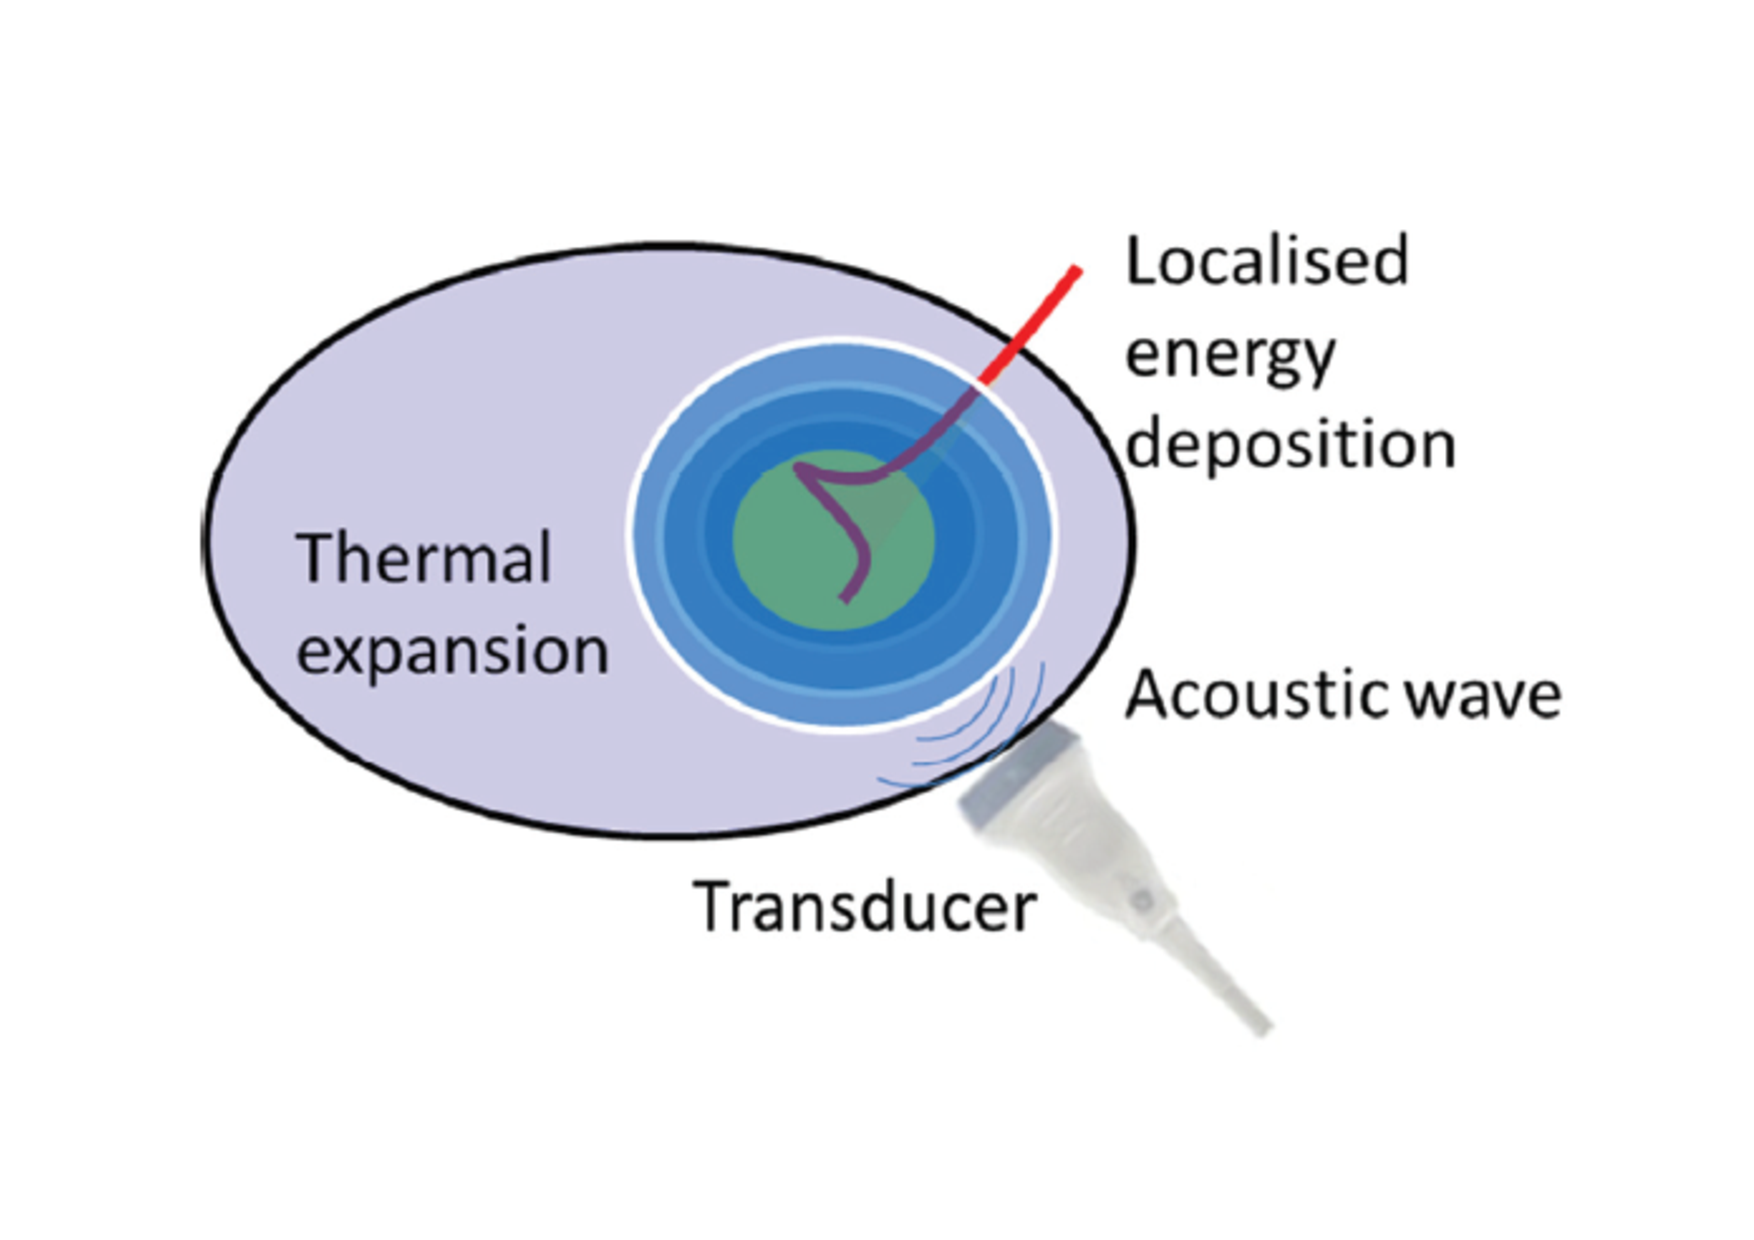
\includegraphics[width=0.98\linewidth]{03_GraphicFiles/chapter1_Introduction/ionoacoustic.pdf}
\caption{Schematic view of the basic principle of iono-acoustic waves detection for ion range verification. In~\cite{Parodi2015b}.}
\label{chap1::fig::ionoacoustic}
\end{subfigure}
\begin{subfigure}[t]{.49\textwidth}
\centering
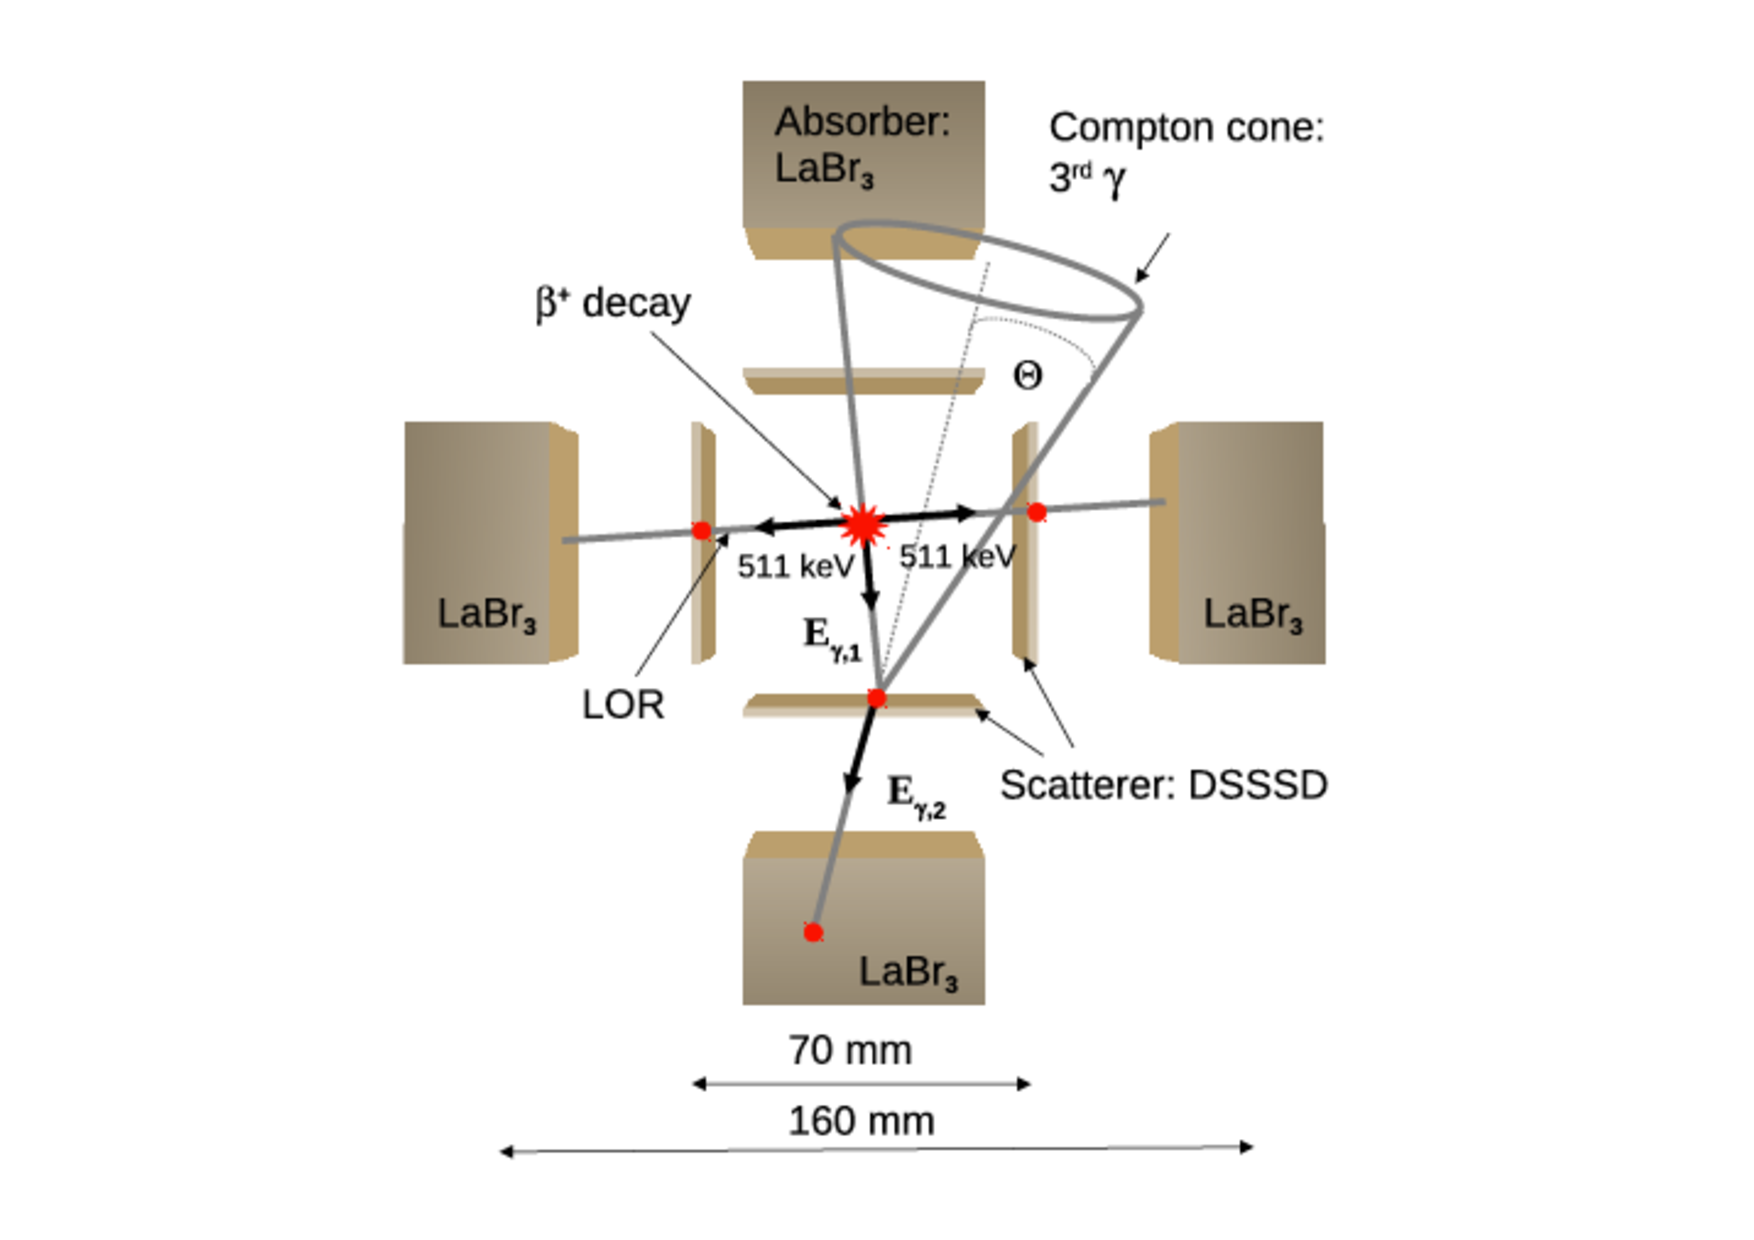
\includegraphics[width=0.92\linewidth]{03_GraphicFiles/chapter1_Introduction/3gamma.pdf}
\caption{Conceptual design of the 3-$\gamma$ detection system proposed in~\cite{Lang2014}, composed of multiple Compton camera arms for the detection of correlated \gls{pet} and de-excitation gammas or \gls{pet} and prompt photons produced in nuclear interactions during particle therapy treatments. In~\cite{Lang2014}.}
\label{chap1::fig::3gamma}
\end{subfigure}
\caption{Alternative methods for in-vivo range verification of ion beam therapy include the detection of iono-acoustic waves produced by the localized dose deposited by the energetic ion beams, whose principle is sketched on the left side, and hybrid systems for 3-photon detection, which can be applied to both nuclear medicine diagnostics and hadrontherapy monitoring, as the one sketched on the right side.}
\label{chap1::fig::alternativeRange}
\end{figure} 

Also water luminescence effects have been verified during the irradiation \myMarginnote{Water luminescence} with proton pencil beams, and are under investigation as a promising solution for range and field width estimations~\parencite{Komori2018}.   
As mentioned, the listed methods have been proposed as alternatives with respect to the more investigated detection of secondary emitted photons, both from positron annihilation and prompt-emission. These two techniques are anyway the most advanced ones, and also hybrid systems are under investigation to obtain a combination of their main advantages and a potential reduction of the identified drawbacks\myMarginnote{Hybrid systems}.  
The so-called \enquote{3-$\gamma$} imaging concept has been explored in France and Germany. The French group combined a standard full ring \gls{pet} scanner with a \gls{tpc} filled with liquid xenon for the Compton measurement~\parencite{Oger2012}, but the detector application is limited to nuclear medicine examinations in its present design. The German group focused on multiple Compton camera heads for the detection in coincidence of positron annihilation photons and de-excitation rays for nuclear medicine applications; such a system can be adapted to perform combined detection of 511~keV photons from $\beta^+$ emission and \glspl{pg}, as already highlighted in~\parencite{Lang2014}. A conceptual detector design for such an application is shown in \figurename~\ref{chap1::fig::3gamma}. Another interesting simulation study applying this \enquote{whole-gamma imaging} concept in nuclear medicine is reported in~\parencite{Yamaya2017b}. 

\newpage

\section{Nuclear medicine}\label{chap1::sec::NuclearMed}

Nuclear medicine is a medical specialty which makes use of particle physics concepts (in addition to medical, biological and chemical knowledge) and instrumentation to study physiological processes and perform non-invasive diagnostic examinations and disease treatments. More specifically, nuclear medicine groups all the medical techniques which foresee the use of chemical compounds containing a radioactive isotope; this radio-pharmaceutical is given to the patient (or mixed to patient samples, for example blood) orally, by injection or by inhalation, and the isotope decay products are used to deliver a treatment dose, for example to cancerous tissues, or for imaging purpose, in case the emitted particles can exit the body and be detected by radiation detectors. 
This thesis focuses on the development of gamma detectors, originally designed for the application in particle therapy; the following sections are devoted to delineate the context in which the studied detectors can be applied for diagnostics, and simulation results of such an application are reported in chapter~\ref{chap::5}.

Some hints about the historical origins of this medical fields have been given in the introduction of this chapter. The use of radioactive isotopes for medical purposes has been investigated since 1920, at the beginning only theoretically, then, since 1940, attempts have been undertaken at imaging radio-nuclide concentration in the human body. The first scan of a radio-nuclide activity in the body was obtained with a very slow planar scanner introduced by Ben Cassen at the beginning of the fifties~\parencite{Blahd1996}, and less than 10 years later Hal Anger developed the first gamma camera, introducing the approach still followed for the modern detectors~\parencite{Anger1958}. The Anger scintillation camera is a planar physically collimated detector which produced two-dimensional projection images of the radio-isotope activity without scanning. The Anger camera, if rotated around the patient, can also be used for tomography, with reconstruction algorithms able to reproduce the three-dimensional emission distribution from two-dimensional multiple-angle slices. The method to reconstruct images from projections had been published by Radon in 1917~\parencite{Radon1917}, and then applied in \gls{ct} and nuclear medicine after 1970. Iterative reconstruction methods were also being investigated, but their application started in the eighties when more computer power became available. The tomographic translation of the Anger gamma camera determined the born of \gls{spect} imaging: together with \gls{pet}, \gls{spect} is still the basis of present diagnostic nuclear medicine. The idea of detecting photon pairs produced by positron annihilation is also attributed to Anger, but the first dedicated \gls{pet} system was built by Ter-Pogossian and colleagues in the 1970s, and employed for phantom and animal studies~\parencite{Ter-Pogossian1975, Ter-Pogossian1983}. Soon afterwards, Phelps, Hoffman and colleagues built the first whole-body \gls{pet}-scanner~\parencite{Hoffmann1976}. 
In the next sections, the physics of radioactive decays is briefly reminded to introduce the detailed discussion of \gls{pet} and \gls{spect} techniques, including a short historical overview, the presentation of the imaging principle and an overview of state-of-the-art machines.
   
\subsection{Radiotracers}\label{chap1::subsec::NMradionuclides}

Nuclear medicine imaging techniques are based on radio-tracers. A tracer is a chemical compound which transports an unstable isotope (radio-nuclide); this molecule is designed to be involved in specific metabolic processes and, thus, to concentrate in the area to be targeted for imaging purpose. The $\gamma$-rays emitted by the radio-nuclide can be measured as a function of position and time, providing anatomical and metabolic information.  In the following, the main physical aspects of radioactive decays are briefly recalled. 

As mentioned, a radio-nuclide is an unstable isotope of a chemical element which decays towards a stable atomic configuration and loses energy by emitting radiation in the form of particles and electromagnetic rays. The decay can involve several steps, if the resulting \enquote{daughters} are still unstable, and the process continues until a stable nuclide is reached. 
Some general features of radioactive decay processes can be detailed mathematically without regard to a specific mechanism. In particular, the decay rate of a sample of radioactive nuclides depends on the nuclides population $N$, according to a decay constant noted as $\lambda$, as expressed by equation~\ref{chap1::eq::decayRate}. 

\begin{equation}\label{chap1::eq::decayRate}
\frac{\mathrm{d}N}{\mathrm{d}t} = -\lambda N 
\end{equation} 

On one hand, the decay constant $\lambda$ is specific of each nuclide, and reflects its degree of instability. The decay rate, on the other hand, is a representation of the sample activity, which is measured in the \gls{si} in Becquerel (1 Bq = 1 disintegration per second) and its multiples, even if an older and still used unit is the curie (Ci) (1 Ci = 3.7 $\times$ 10$^{10}$ disintegration per second). The solution of the differential equation in~\ref{chap1::eq::decayRate} gives the number of parent atoms $N$ at any time $t$, or the activity by multiplying both side by $\lambda$:

\begin{equation}\label{chap1::eq::parentAtoms}
\begin{split}
N = N_{0}e^{-\lambda t}  \\
A = A_{0}e^{-\lambda t}  \\
\end{split}
\end{equation} 

with $N_0$ and $A_0$ the original number of parent atoms and the original activity, respectively. Following these first expressions, the physical half-life $T_{1/2}$ of a radioactive nuclide is the time required for the decay of half of the atoms in a sample; its mathematical form is reported in equation~\ref{chap1::eq::half-life}.

\begin{equation}\label{chap1::eq::half-life}
T_{1/2} = \frac{\mathrm{ln}2}{\lambda} = \frac{0.693}{\lambda}
\end{equation} 

Several decay modes exist, and they can be divided into three main categories: emission of nucleons (protons and neutrons), emission or capture of electrons, emission of photons. In particular, five main decay channels have been identified (see \figurename~\ref{chap1::fig::nuclides}):
\begin{itemize}
\item $\alpha$-decay;
\item electron emission - $\beta^-$-decay;
\item electron capture (electron captured from the inner shells of the atom);
\item positron emission - $\beta^+$-decay;
\item isomeric transition: gamma emission and internal conversion (electron emission).
\end{itemize}
In \figurename~\ref{chap1::fig::decayScheme} the decay scheme of a generic nuclide $^{A}_{Z}X$ is depicted (A is the atomic mass, Z the number of protons); the $\alpha$-decay produces $^{A-4}_{Z-2}P$, electron capture and positron emission equivalently generate $^{A}_{Z-1}Q$, while $^{A}_{Z+1}R$ originates from electron emission and can be created in a metastable configuration $^{A}_{Z+1}R^*$ which then decays to the stable state via isomeric transition with the emission of a photon.  

\begin{figure}[!htbp]
\begin{subfigure}[t]{.35\textwidth}
\centering
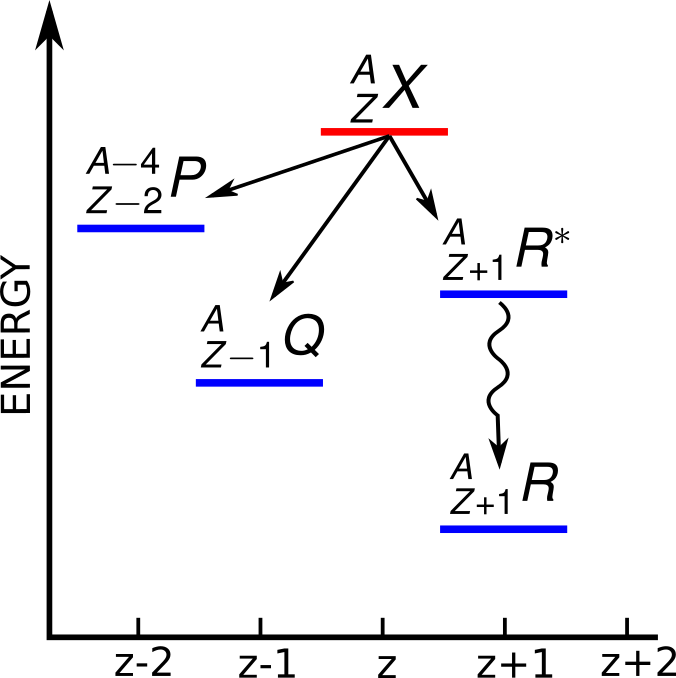
\includegraphics[width=0.9\linewidth, trim={0 4cm 0 3cm}, clip]{03_GraphicFiles/chapter1_Introduction/decayScheme.pdf}
\caption{Radioactive decay scheme. In~\cite{Hendee2002}}
\label{chap1::fig::decayScheme}
\end{subfigure}
\begin{subfigure}[t]{.64\textwidth}
\centering
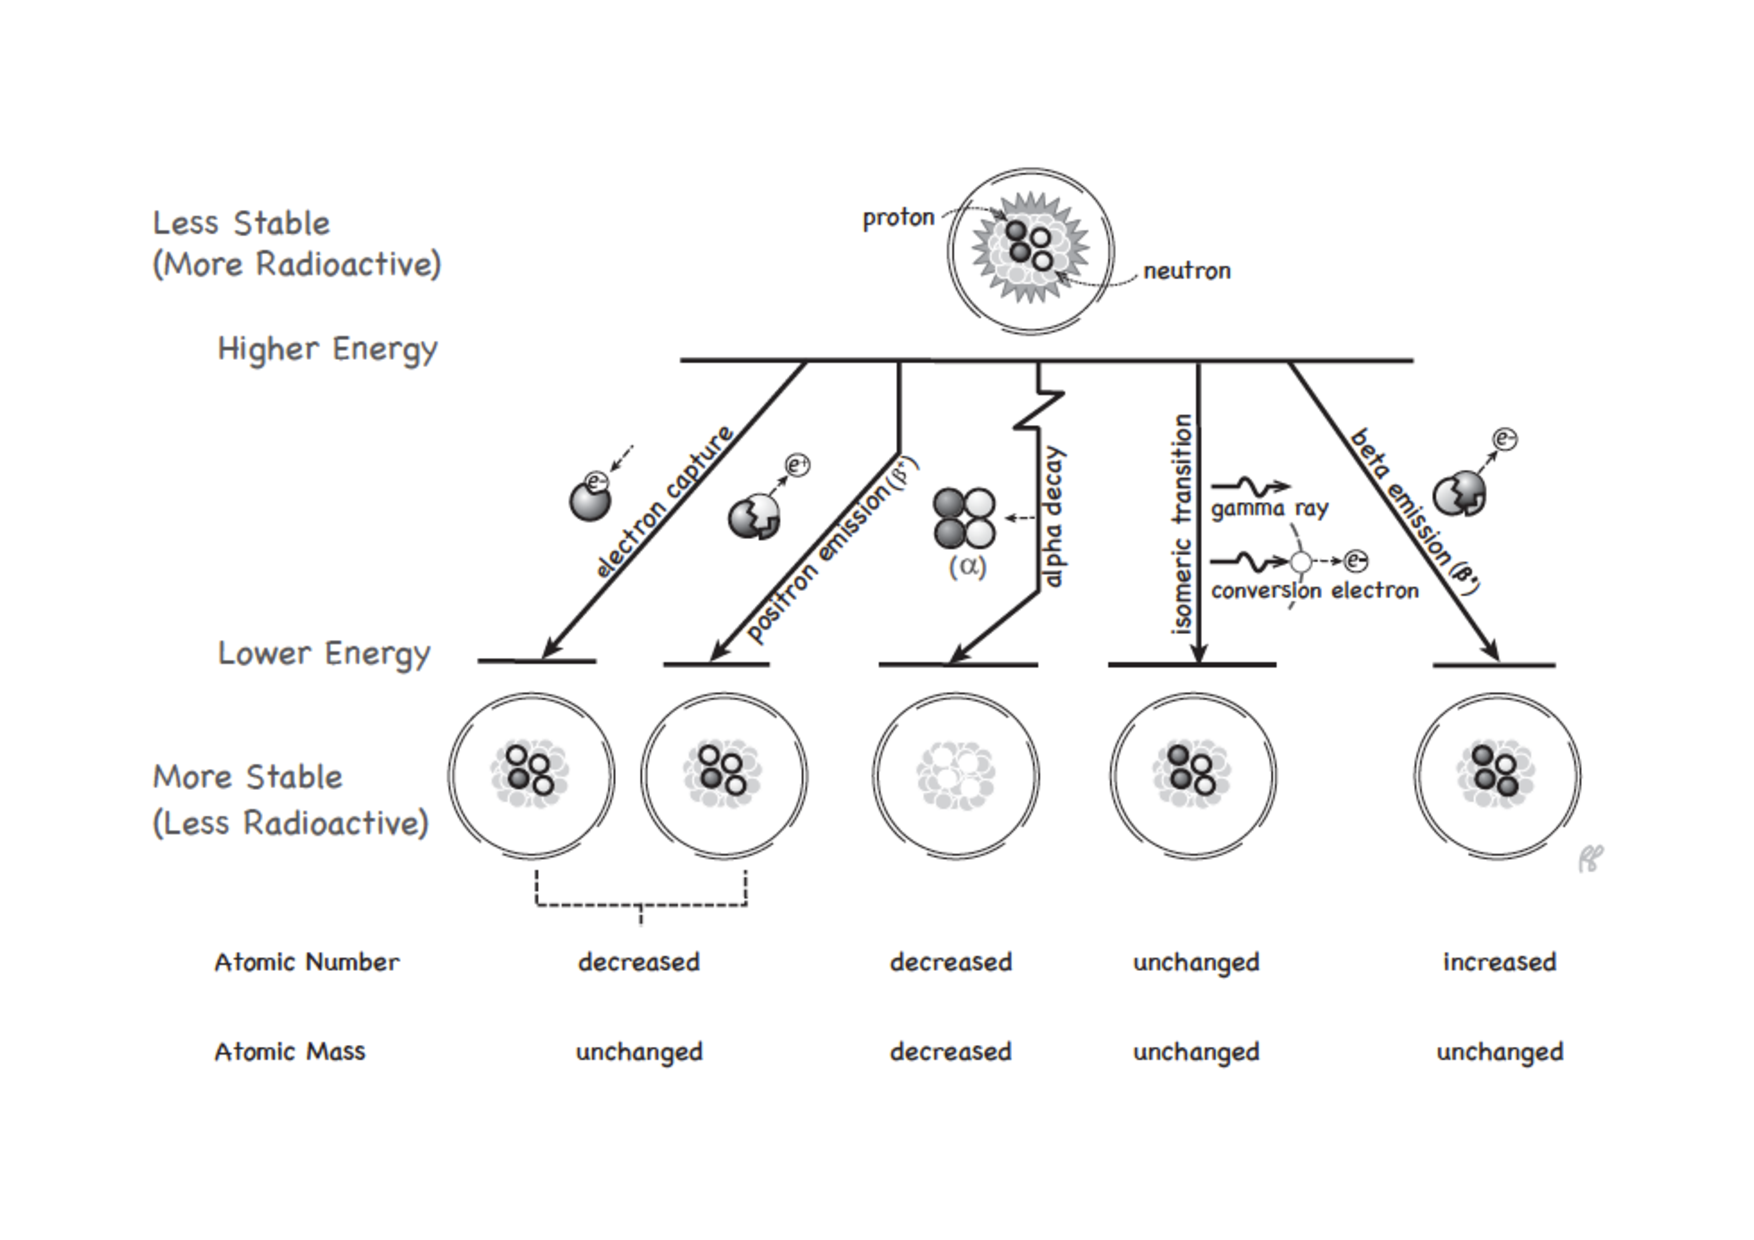
\includegraphics[width=0.98\linewidth]{03_GraphicFiles/chapter1_Introduction/decaySchematicSimple.pdf}
\caption{Schematic view of the radioactive decays. In~\cite{Powsner2013}.}
\label{chap1::fig::nuclides}
\end{subfigure}
\caption{The various radioactive decay channels are schematized in (a) for a generic isotope $^{A}_{Z}$X. A more detailed scheme, describing the decay processes and products, is given in (b).}
\label{chap1::fig::radioactiveDecay}
\end{figure} 

The $\alpha$-decay \myMarginnote{$\alpha$-decay} is the spontaneous emission of an $\alpha$ particle (i.e. an helium nucleus, consisting of two protons and two neutrons), typically from heavy nuclides (A > 150). It was discovered by Marie and Pierre Curie in 1989~\parencite{Curie1898} and first described by Rutherford one year later~\parencite{Rutherford1899}, who also identified the $\alpha$ particles as helium nuclei, together with Boltwood in 1911~\parencite{Boltwood1911}. The decay can be described by equation~\ref{chap1::eq::alphaDec}. Often it is followed by the emission of characteristic x-ray or gammas, accompanied by competing processes of internal conversion and Auger electron emission. The produced $\alpha$ particles have energies in the range 2-10~MeV and are not used for imaging purposes, given the very limited range in tissues (about 100~\charmum). This characteristic makes such a decay appropriate for therapy, even if the very short decay time is a limiting factor. Only the $\alpha$-decay of a few high-Z elements is actually used, for example, for tumor irradiation in the so-called \enquote{internal radiotherapy} or \enquote{brachytherapy}~\parencite{Suntharalingam2005, Dahiya2016}. 

\begin{equation}
^{A}_{Z}X \, \rightarrow \, ^{A-4}_{Z-2}Y + ^{4}_{2}\mathrm{He} + \mathrm{energy}
\label{chap1::eq::alphaDec}
\end{equation} 

The decay via emission of an electron \myMarginnote{Electron emission} ($\beta^-$- or negatron-decay) can be seen as the conversion of a neutron in a proton and an electron-anti-neutrino pair, as in the generic reaction reported in equation~\ref{chap1::eq::electronEmiss}.

\begin{equation}\label{chap1::eq::electronEmiss}
\begin{split}
^{A}_{Z}X \, \rightarrow \, ^{A}_{Z+1}Y + e^{-} + \overline{\nu} + \mathrm{energy} \\
n \, \rightarrow \, p + e^{-} + \overline{\nu} 
\end{split}
\end{equation}   
 
This decay channel pertains to nuclei with a N/Z ratio (with N the number of neutrons) too high for stability and results in nucleus with Z increased by one, N decreased by one and so the same atomic mass A (isobaric transition) but a different chemical element. $\beta^-$-decay pathways are characterized by specific maximum energies $\mathrm{E_{max}}$ for the emitted electron, with an average value of approximately 1/3 $\mathrm{E_{max}}$; the remaining energy is carried away by the anti-neutrino. This results in poly-energetic energy spectra for the emitted electrons. The difference in the energy released during decay and the one possessed by the emitted electron threatened the energy conservation law for years. In 1930, in a letter, Wolfgang Pauli suggested that a second particle was emitted during the decay, explaining the energy, momentum and angular momentum conservation. The name neutrino was attributed to such a particle by Enrico Fermi. 
Any possible excess energy in the nucleus after the decay (metastable state) is emitted as gamma rays or internal conversion electrons. As for the $\alpha$ particle case, electrons have limited range in matter, thus release dose to the tissues, and have no diagnostic value (but they are used in brachytherapy), but metastable states deriving from $\beta^-$-decays are pure sources of $\gamma$-rays and are so employed for imaging. One of the most diffused tracer is a metastable daughter of $^{99}$Mo, the $^{99m}$Tc; it decays in stable $^{99}$Tc (half life = 6 hours) by emitting a 140~keV photon.   

On the other side of the \enquote{nuclide stability line}, \myMarginnote{Positron emission} neutron-poor radionuclides (with low N/Z ratio) tend to decay by the emission of a positron ($\beta^+$ decay) and to increase the neutron number by one. As shown by equation~\ref{chap1::eq::positronEmiss}, the net result is the conversion of a proton into a neutron with the ejection of a neutrino, in addition to the positron. As in the previous case, the transition is isobaric because the total number of nucleons is unchanged.

 \begin{equation}\label{chap1::eq::positronEmiss}
\begin{split}
^{A}_{Z}X \, \rightarrow \, ^{A}_{Z-1}Y + e^{+} + \nu + \mathrm{energy} \\
p \, \rightarrow \, n + e^{+} + \nu 
\end{split}
\end{equation}     

The emission of positrons was discovered in 1933 by the Marie Curie daughter Irene Curie and her husband Frederic Joliet, in bombardments of aluminium by $\alpha$ particles~\parencite{Leone2010}. Even if the reaction principle is similar to $\beta^-$-decay, an important difference resides in the behavior of the decay product. Both electron and positron undergo energy deposition processes by excitation and ionization, but if electrons can be captured by atoms (or absorbed in free electron bands) when they come to rest, positron react with their antiparticle (electron) by annihilation. The entire rest mass of the particle pair is converted to energy and emitted as two back-to-back 511~keV photons for conservation laws. The annihilation takes place in a time window of about 1~ns after the $\beta^+$-decay, and within a few millimeter of the decay site (depending on the medium). This kind of reaction is the basis of one of the most diffused nuclear medicine imaging technique, the \gls{pet}, discussed in section~\ref{chap2::subsec::PET_NM}. An example of a positron emitter used in imaging is $^{18}$F, with a half-life of 109 minutes.
To be noticed that, as for $\beta^-$-decay, the daughter nucleus can further emit photons to lower its energetic level, which can be used in combined imaging techniques (three-$\gamma$ imaging).
The N/P ratio of neutron deficient nuclides can also be increased via \gls{ec} reactions \myMarginnote{\gls{ec}}; the nucleus can capture an orbital electron and convert a proton into a neutron, with the consequent emission of a neutrino. This phenomenon is described by equation~\ref{chap1::eq::electronCapture}.

 \begin{equation}\label{chap1::eq::electronCapture}
\begin{split}
^{A}_{Z}X + e^{-} \, \rightarrow \, ^{A}_{Z-1}Y  + \nu + \mathrm{energy} \\
p + e^{-}\, \rightarrow \, n  + \nu 
\end{split}
\end{equation}     

Most electrons are captured from the K shell, more uncommon are the capturing processing involving L shell or even shells farther from the nucleus. As a result of the capture, a vacancy is created and filled by an electron from an higher-energy shell. This transition leads to a reduction of the atomic rest energy, and the release of characteristic x-rays and/or Auger electrons. As with other modes of decay, further $\gamma$-rays can be emitted if the daughter nucleus is left in an excited state after the capture process. An example of electron capture decay is represented by $^{201}$Tl, which decays to $^{201}$Hg with the emission of K-x-rays of 69-83 keV (98\% abundance) and photons of 135 and 167~keV in 10\% total abundance. Many nuclei decay by both electron capture and positron emission, as for example the $^{22}$Na.
As mentioned for the previously described decay modes \myMarginnote{Isomeric transition - $\gamma$-decay}, often the daughter nucleus is formed in an excited state, which is still unstable. The transition towards a condition of stability entails an internal atomic re-arrangement and the emission of $\gamma$-rays at characteristic energies. In general, such a transition is almost instantaneous, but some excited states can persist for longer periods, with half-lives which ranges on several orders of magnitude, between 10$^{-6}$~s and hundreds of years. The decay of this kind of nuclei, called metastable or isomeric, is called isomeric transition, and only results in the $\gamma$-ray emission with no emission or capture of other particles by the nucleus. A complementary pathway for the energy release is represented by the interaction of the nucleus with an atomic electron; this process is called \gls{iconv}, and the involved electron is ejected. This emission is further followed by x-rays and Auger electron emission, so that the atom can resume a stable state. The isomeric transition is described by equation~\ref{chap1::eq::isomericTrans}, where the letter $m$ indicates the metastable state.

 \begin{equation}\label{chap1::eq::isomericTrans}
^{Am}_{Z}X  \, \rightarrow \, ^{A}_{Z}X  + \mathrm{energy} \\
\end{equation}        

To be noticed that no radioactive nuclide decays solely by an isomeric transition, which is always preceded by another decay mode. In addition to the already mentioned decay of $^{99m}$Tc, deriving from the previous decay of $^{99}$Mo, also $^{60}$Co decays in excited $^{60}$Ni nuclei which then reach the ground energy state by isomeric transition with the emission of 1.17 and 1.33~MeV photons. 
In table~\ref{chap1::tab::Isotopes_NM} some of the radioisotopes typically used for imaging and therapy are listed with their half-life and common uses. 

\begin{table}[!htbp]
\centering
\caption{Commonly-used radioisotopes for the clinical imaging and therapy routine. Table adapted from~\cite{Ruth2009}.}
\label{chap1::tab::Isotopes_NM}
\resizebox{\textwidth}{!}{%
\begin{tabular}{clll}
\toprule
\rowcolor{myColorMainA!20} 
\textbf{Application} & \textbf{Radioisotope}& \textbf{Half-life} & \textbf{Details} \\
\midrule
\multirow{12}{*}{\STAB{\rotatebox[origin=c]{90}{Imaging}}}& Technetium-99m & 6 h (from $^{99}$Mo 66 h)    &  Used to image the almost all the body, skeleton and heart muscle in particular.\\
& Cobalt-57             & 272 d                                        & Used as marker to estimate organ size and for \textit{in vitro} diagnostic kits.\\
& Gallium-67           & 78 h               						    & Used for tumor imaging and localization of inflammatory lesions.\\
& Indium-111           & 67 h     								    & Used for specialist diagnostic studies and colon transit studies.\\
& Iodine-123           & 13 h      								    & Used for diagnosis of thyroid function.\\
& Krypton-81m       & 13 s (from $^81$Rb 4.6 h)	    & Used in gas status for images of pulmonary ventilation and in general for lung applications.\\
& Rubidium-82       & 65 h          							    & Convenient \gls{pet} agent for myocardial perfusion imaging.\\
& Thallium-201       & 73 h  									    & Used for diagnosis of coronary artery disease and other heart studies.\\
& Carbon-11           & 20.4 m 								    & \\
& Nitrogen-13        & 9.97 m  								    & Positron emitters used in \gls{pet} for studying brain physiology and pathology.\\
& Oxygen-15          & 2 m    								        & They also have a significant role in cardiology.\\
& Fluorine-18         & 110 m									   & \\ 
\midrule
\multirow{4}{*}{\STAB{\rotatebox[origin=c]{90}{Therapy}}}& Bromine-77         & 2.4 d                                            & Auger electrons decay mode.\\
& Palladium-103     & 17.5 d                                          & Auger electrons decay mode.\\
& Rhenium-186      & 90.6 h                                         & $\beta^-$-decay mode.\\
& Astatine-211       & 7.2 h               						   & $\alpha$-decay mode.\\
\bottomrule
\end{tabular}}
\end{table}    

Although many naturally occurring radioactive nuclides exist\myMarginnote{Radionuclide production}, all of those commonly administrated to patients in nuclear medicine tracers are produced artificially in order to fit the clinical requirements. Artificial induced radioactivity was introduced by the already mentioned Irene Curie and his husband, who bombarded aluminum targets with $\alpha$ particle~\parencite{Leone2010}. Nowadays, most radionuclides are produced with cyclotrons and nuclear reactors, and radionuclide generators are used to \enquote{store} short-life isotopes. In general, $\beta^-$ emitters are produced by bombarding stable nuclei with neutrons from nuclear reactors, while $\beta^+$-decay nuclides are produced with bombardment with protons, helium ions, deuterons or tritons accelerated with cyclotrons (see section~\ref{chap1::subsubsec::accelerators} for the description of the cyclotron). In other cases, radionuclides are produced as by-products of fission in nuclear reactors, or as decay product of other isotopes produced with one of the listed methods. 
In the cyclotron-based production, the accelerated ions collide with the target nuclei causing nuclear reactions, presented in section~\ref{chap1::subsubsec::ionInteractions}. As explained, fragmentation processes can create radioactive nuclei, such as $\beta^+$ emitters, employed in \gls{pet} diagnostics. In general, cyclotron facilities must be in close proximity to the hospital where the produced radionuclides will be administrated because of their short half-life. $^{18}$F, created with this technique as product of nuclear reactions with $^{18}$O, is an exception in this sense, with an half-life of 109 minutes. 
In nuclear reactors, two techniques are exploited: nuclear fission and neutron activation. The absorption of neutrons from nuclear reactors can induces fission processes in heavy nuclei, which split in lighter (often unstable) ones. Its long half-life makes $^{235}$U the most widely used fissile element; when it absorbs a neutron, the resulting state of $^{236}$U is unstable and in most cases it promptly splits into its fission fragments. For example, $^{99}$Mo has already been mentioned as the parent nucleus for the production of  $^{99m}$Tc and derives by the fission of uranium. Another widely used nuclide produced with fission procedure is the $^{131}$I. The creation of the fission fragments is very often accompanied by the emission of secondary neutrons which can be used to create other nuclides by neutron activation. Stable nuclei, indeed, can capture neutrons and produce, in most cases, $\beta^-$ emitters, as the $^{32}$P or the $^{50}$Cr. In some cases, the sample activity reached with such a production technique is not sufficient, because stable nuclei are still present among the parent atoms, and so fission mechanisms are preferred. 
The last mechanism involves radionuclide generators, particularly interesting for short half-life nuclides. In order to solve the supply problem for short-living isotopes, the sample is often prepared with the longer-living parent nuclide (the so-called \enquote{generator}), which then decays in the desired one continually providing it. This is for example the case of the most important radio-nuclide used in a variety of application, $^{99m}$Tc, result of the decay of $^{99}$Mo. 

Once produced, the radioactive nuclei must be attached \myMarginnote{Radiotracer features} to appropriate substances providing the desired biological properties, for example to be preferentially absorbed in the target region. The final product, ready to be administrated to the patient, is called \enquote{radiotracer}. 
For diagnostics, the selected radioisotope half-life should be short enough so that a considerable part of the decays occurs during the examination time; any radiation released after the end of the examination is a source of useless dose to the patient. The dose delivered after the end of the treatment can be reduced if the biological excretion, guaranteed by the tracer characteristics, is rapid. Always focusing on diagnosis, the optimal decay scheme is the pure $\gamma$-decay, with an isomer as radionuclide; anyway, the amount of produced non-penetrating radiation should be minimized. The exception is represented by $\beta^+$ emitters, resulting in the positron annihilation 511~keV photons exploited by \gls{pet} techniques. In addition to this, the produced photon energy must be considered: nowadays, the majority of scintillation cameras are optimized for energies close to 140~keV (main emission of $^{99m}$Tc), which is a compromise among patient attenuation, spatial resolution and detection efficiency. Photons at lower energies are largely attenuated and increase the patient dose without contributing to the image formation. High-energy photons escape the body and deliver a minimal dose to the patient, but the present machines have poor detection efficiency in such an energy range, and the physical collimators are not optimized; both these factors result in image quality degradation. High-energy photons can be used if new detector solutions are explored, like the one presented in chapter~\ref{chap::5}. 
For therapy non-penetrating radiation are requested and must be maximized, and correlated photon emission can be in principle used for dosimetric verification, in the so-called theranostics approach~\parencite{Yordanova2017}. 
From the biological point of view, \enquote{hot spots} (in which the tracer is more concentrated than in other regions) are desired for therapy, while for diagnosis it is possible to profit from both \enquote{hot} and \enquote{cold spots}. Several mechanisms can be implemented in order to concentrate the radiotracer in the target area. Localized administration of the radiotracer in the target region is the first option, while with active transport techniques, the tracer is concentrated into specific organ against concentration gradients thanks to cellular metabolic processes.  The glucose metabolism is also exploited, for example for the \gls{fdg} tracer used in 85\% of the \gls{pet} clinical practice. The tracer size is fundamental in techniques based on the phagocytosis by specialized cells or on traps in specific organs. Very large molecules (20-40~\charmum diameter) can concentrate in capillaries with smaller diameter. An irregular diffusion through tissue membrane can also be used to identify lesions if specific tracers are employed. Chemotaxis (the movement of a cell in response to chemical stimulus) can also promote the migration and accumulation of radiotracers, for example as part of an overall inflammatory response. Moreover, some radio-pharmaceuticals are produced with specific characteristics which provide them high affinity to bind to receptor sites, for example in tumors. Finally, the blood flux can be used for blood specific studies. 

The choice of the radiotracer depends on the specific organ or region of the body to be examined and on the chosen detection technique. As already detailed, on one side \gls{pet} aims to detect the two back-to-back photons produced by the annihilation of a positron emitted by the radio-isotope and an electron of the patient body. On the other side, \gls{spect} detects single photons, and the spatial localization is given by mechanical collimation systems. In both cases, tomographic reconstruction is foreseen to obtain three-dimensional images.

The physical basis, historical development and present status of these two techniques are detailed in section~\ref{chap2::sec::GammaNM}. In addition, the theranostics approach, aiming to perform combined diseases radiation treatment and diagnosis and/or verification imaging, is also addressed in section~\ref{chap2::subsec::Theranostics}.  
 
%\subsection{Positron Emission Tomography}\label{chap1::subsec::PET_NM}
%
%PET systems rely on the detection of annihilation gamma rays that follow positron decay of the radioisotope injected in the patient and consequent positron annihilation. The gamma rays exiting the patient body are detected in coincidence by scintillating detectors surrounding the patient, and the distribution of positron emitters is retrieved \textit{in vivo}. 
%\figurename~\ref{chap1::fig::NM_PET_princ} shows the principle at the basis of \gls{pet} imaging. 
%
%\begin{figure}[!htbp]
%\centering
%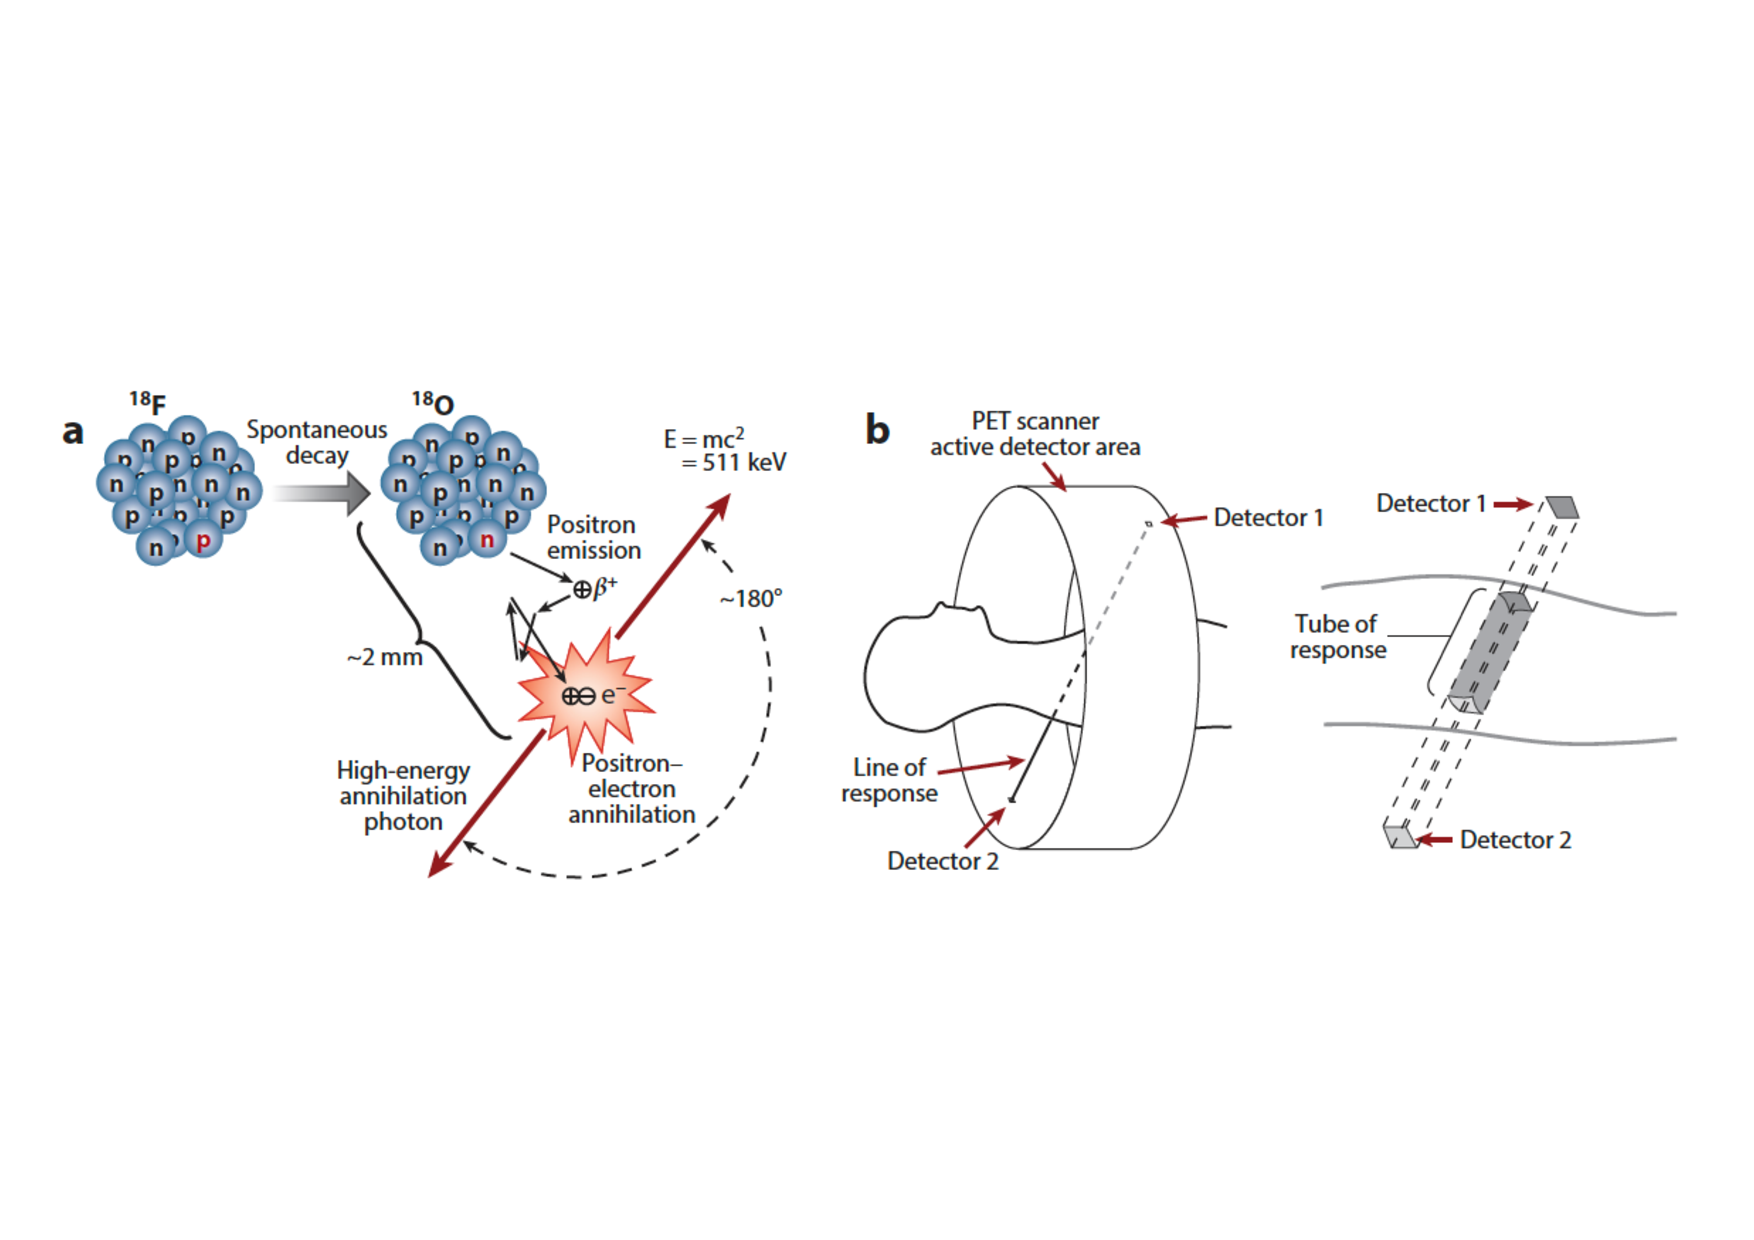
\includegraphics[width=0.8\textwidth, trim = {0 3cm 0 3cm}, clip]{03_GraphicFiles/chapter1_Introduction/NM_PET_principle.pdf}
%\caption{The $\beta^{+}$ decay of $^{18}$F creates the stable isotope $^{18}$O and a positron, which travels short distance (1-2~mm) before interacting with an electron. The consequent annihilation produces two anticollinear 511~KeV photons (a). The two photons are detected by the \gls{pet} scanner in time coincidence, and the two points of interaction defines a line of response, then extended to a so-called \enquote{tube of response} which accounts for the detector's elements finite dimensions (b). In~\cite{Vaquero2015}.}
%\label{chap1::fig::NM_PET_princ}
%\end{figure}   
%The two annihilation photons are typically detected with time coincidence windows ranging between 1 and 10~ns, depending on the specific features of the employed scanner. The spatial resolution of \gls{pet} imaging is intrinsically limited by the fundamental nature of positron annihilation, if we consider that after its creation, the positron can travel a few millimeters and follow a tortuous path through the tissue (mainly due to Coulomb scattering with electrons which can occur at large angles given the fact that the rest mass of positron is the same as the one of the electron) before reaching thermal energies and annihilating. In addition to the positron range, also the variation in the momentum of the positron leads to a limitation of the spatial resolution of \gls{pet} images. Indeed, such a variation results in an angular uncertainty in the direction of the two annihilation photons known as \enquote{noncolinearity}. Moreover, significant limitations are linked to the employed detector: the coincidence detector-pair resolution is normally specified as the \gls{fwhm} of the \gls{psf} obtained from the convolution of the two individual detector \glspl{psf}. For a detector composed of small discrete crystals, the interactions are generally assumed to take place at the center of individual crystals, and the resulting \gls{fwhm} of the coincident detector \gls{psf} is one-half the crystal size. A further factor affecting \gls{pet} imaging resolution is the parallax error, which results form the uncertainty of the \gls{doi} of the gamma rays in the crystal. Thus, unless the \gls{doi} within a crystal can be accurately determined (dedicated designs are needed), an incorrect \gls{lor} will be assigned to the interaction. A schematic representation of the parallax error is provided in \figurename~\ref{chap1::fig::PET_parallax}. The parallax error is all the more increased when the \gls{pet} ring diameter is reduced of the thickness of the crystals is increased, as the relative thickness of the detector increases. 
%
%\begin{figure}[!htbp]
%\begin{subfigure}[t]{.49\textwidth}
%\centering
%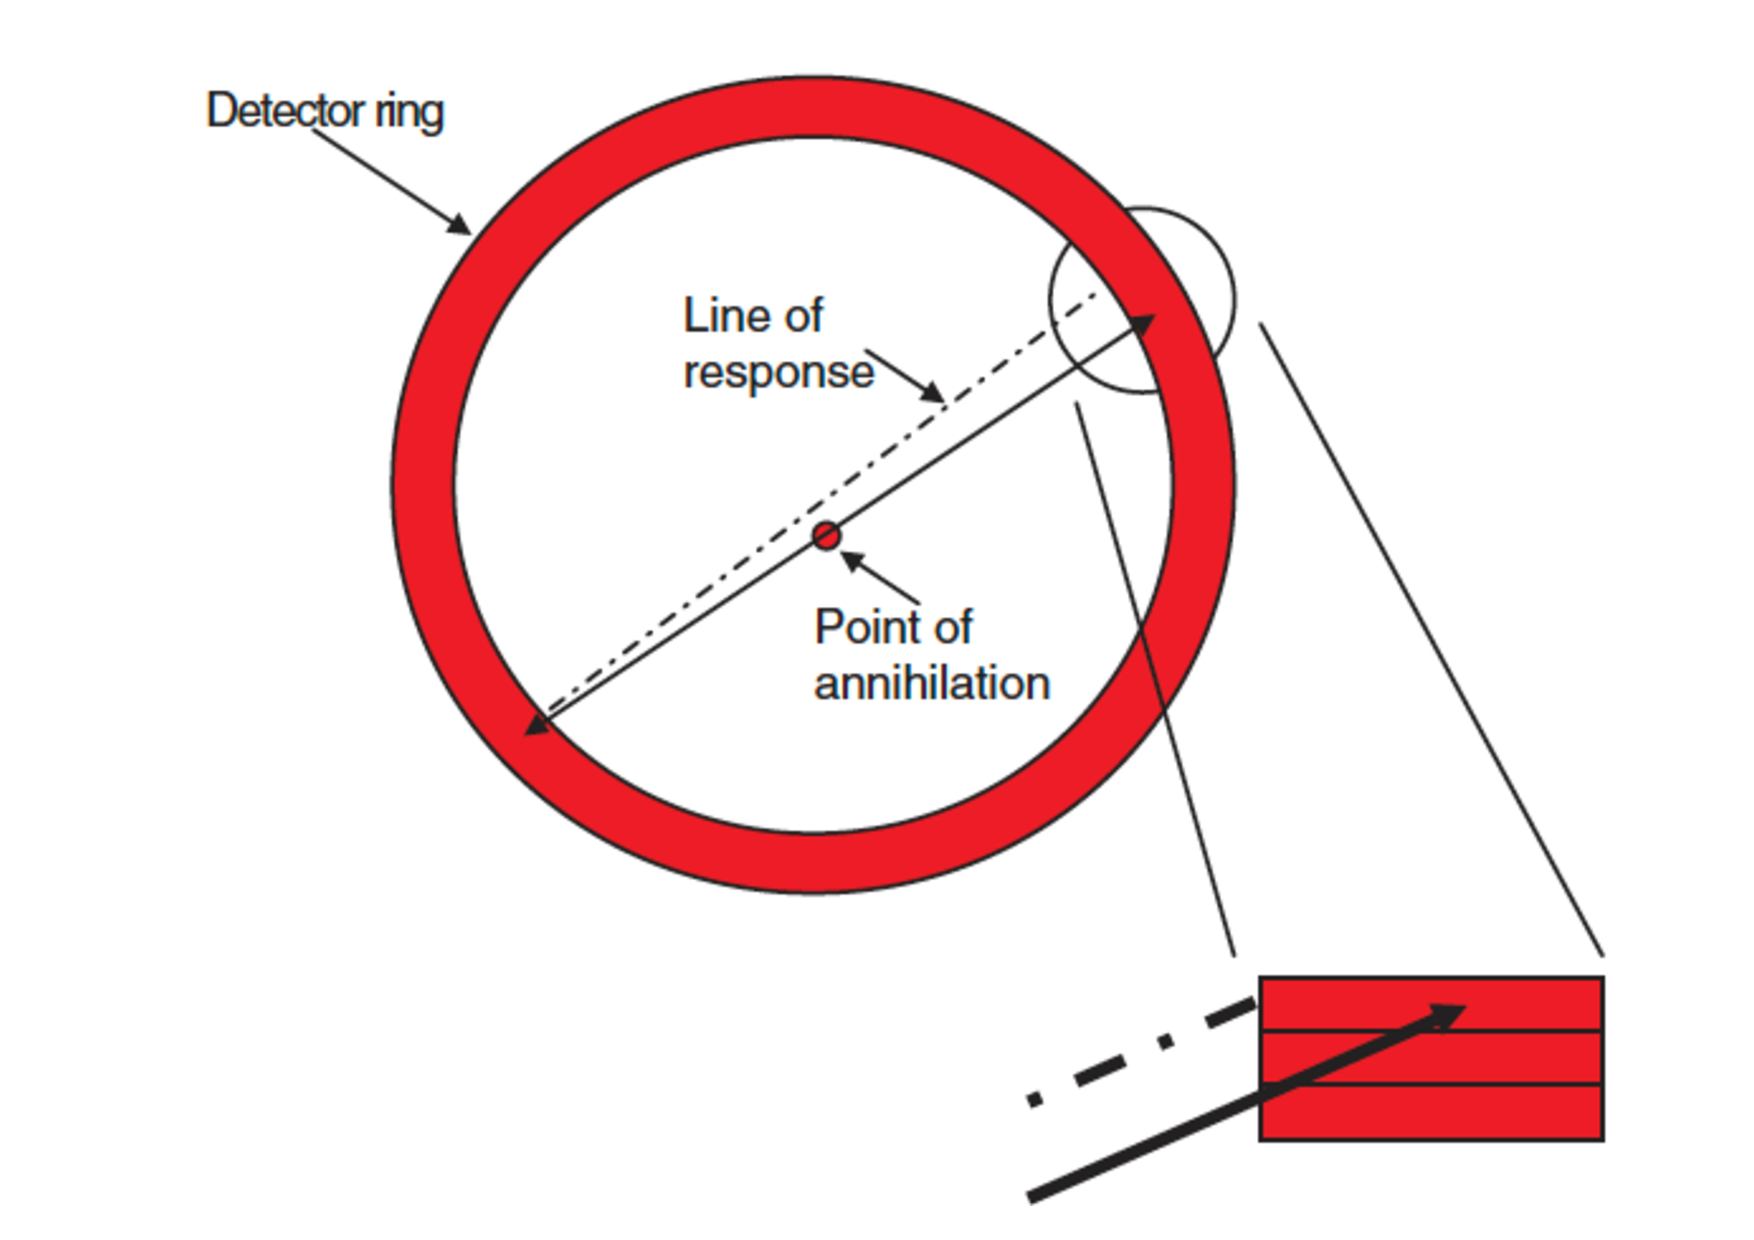
\includegraphics[width=0.7\linewidth]{03_GraphicFiles/chapter1_Introduction/PET_parallax.pdf}
%\caption{Schematic view of the parallax error. The gamma ray (solid line) interacts in a crystal after penetrating one or more adjacent crystals in the detector ring. The detection electronics, if \gls{doi} information is not accessible, will incorrectly assign the \gls{lor} (dotted line) based on the front of the interaction crystal.}
%\label{chap1::fig::PET_parallax}
%\end{subfigure}
%\begin{subfigure}[t]{.49\textwidth}
%\centering
%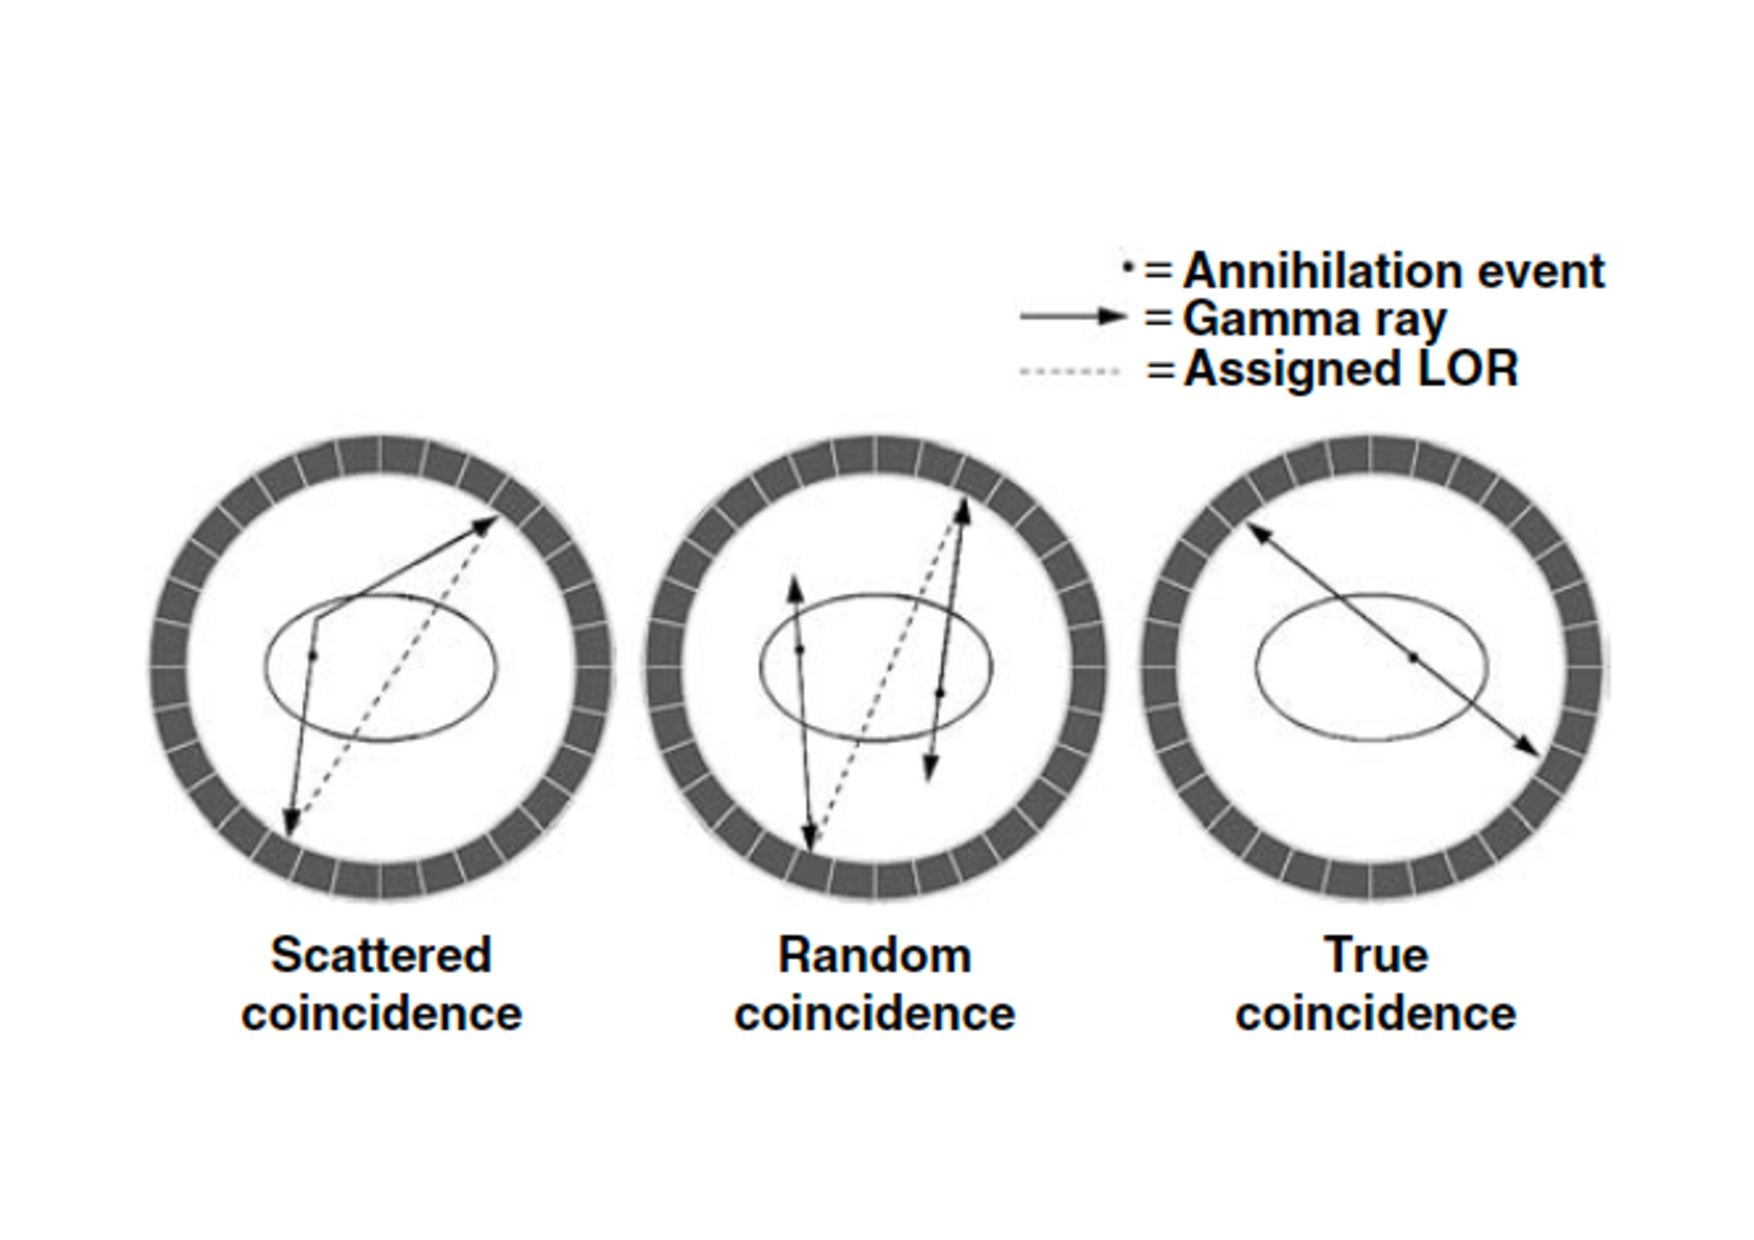
\includegraphics[width=0.98\linewidth]{03_GraphicFiles/chapter1_Introduction/PET_events.pdf}
%\caption{The three types of coincidence events measured in a \gls{pet} scanner.}
%\label{chap1::fig::PET_events}
%\end{subfigure}
%\caption{In~\cite{Lewellen2004}.}
%\label{chap1::fig::PET_details}
%\end{figure} 
%
%\figurename~\ref{chap1::fig::PET_events} shows the three kinds of coincidence events that a standard \gls{pet} accepts: 
%\begin{itemize}
%\item true coincidences: gamma rays are detected from a single decay that have not scattered in the patient;
%\item scattered events: one or both gamma rays scatter within the patient;
%\item random coincidences: two separate decays result in the detection of only one gamma rays from each one and the two events are close enough in time to be in coincidence.
%\end{itemize}
%It is clear that increasing the number of true coincidences leads to less noise in the final image and allows one to reconstruct the collected data with high spatial resolution, and the effect of scattered coincidences can be corrected at the reconstruction stage, as well as the attenuation effect in the patient. The random coincidences are hardly treated, but their number can be reduced by decreasing the injected radiotracer activity.
%
%The origin of the \gls{pet} imaging modality dates back to the beginning of the 50s, when a simple brain probe was used to localize brain tumors by detecting photon coincidences with 2 opposing \gls{naitl} detectors at the \gls{mgh}~\parencite{Sweet1951}. In the same year, a similar approach was published on \textit{Science} by a second reserach group~\parencite{Wrenn1951}. The development of reconstruction techniques for tomographic imaging started in the early 1960s~\parencite{Kuhl1963}, and in parallel to the first clinical trial for x-ray computed tomography the \gls{mgh} physics group developed the \gls{fbp} technique~\parencite{Chesler1971}. The first ring tomograph was built in 1973 by Robertson of \gls{bnl}, and it was composed of 32 detectors disposed in a circular array~\parencite{Robertson1972}. One year later, the PETT I (Positron Emission Transaxial Tomography) tomograph prototype was built at the Washington University by Michael E. Phelps: such a prototype was then upgraded until a human-size system, called PET III, which included extended reconstruction not limited to the transaxial plane. The system consisted of an hexagonal array with 48 \gls{naitl} detectors, and of a gantry allowing for a 60-degree rotation. With this system, the first human \gls{pet} images using the \gls{fbp} algorithm were produced~\parencite{Hoffmann1976}, marking the beginning of modern \gls{pet} development. Following the PET III development, the first commercial \gls{pet} scanner, named ECAT II (Emission Computed Axial Tomograph), was designed and put on the market; it was composed of 96 \gls{naitl} crystals, and it had a dedicated computer. The transition to commercial systems continued in the following years, and it boosted the establishment of worldwide \gls{pet} research programs. Another fundamental step in the development of the \gls{pet} technology was the discovery of \gls{bgo} scintillator. The first scanners were all based on \gls{naitl}, difficult to manufacture because of its hygroscopic nature, and with a low density, thus limited efficiency in detecting 511~keV gamma rays.  The luminescence features of \gls{bgo} were first studied by Weber at the University of California~\parencite{Weber1973}, and Nester and Huang characterized the \gls{bgo} scintillation properties in 1975~\parencite{Nestor1975}. These studies leaded to the first design and construction of a \gls{bgo}-based \gls{pet} scanner in 1978, and right after to the commercialization of the NeuroECAT, the first commercial machine to use \gls{bgo} as scintillating material. Hundreds of \gls{bgo}-based tomographs have been produced since the first introduction. 
%The availability of commercial valuable \gls{pet} scanners was only one of the factor determining the spread of this imaging technique: in parallel, the development of optimized radiotracers was the second key point. Since the beginning of the \gls{pet} experience and until the second half of the 1970s, the images were obtained mainly using $^{11}$C-glucose, $^{15}$O-water and $^{13}$N-ammonia for blood flow, $^{15}$O-oxygen for oxygen utilization, and $^{18}$F fluoride for bone scans. In addition, successful molecular imaging probe was derived from the $^{14}$C-deoxyglucose. The synthesis of $^{18}$F-tagged deoxyglucose was discussed already at the beginning of the 1970s, and the Brookhaven group (Al Wolf and Joanna Fowler in particular), synthesized the first \gls{fdg}~\parencite{Ido1978}. Refined synthesis methods were developed in the following years, also thanks to the improvements of cyclotron accelerator technology, allowing for a routine basis tracer production. Nowadays, a number of companies provide small cyclotrons with various forms of automated chemistry for producing molecular imaging probes, and \gls{fdg} is still the most employed one for modern clinical \gls{pet} imaging.
%During the 1980s, particular focus was dedicated to the detector side, with the development of the so-called \enquote{block detectors}: the new optical multiplexing scheme permitted to use many small scintillator pixels on a small number of \glspl{pm}, and so provided high granularity (and spatial resolution) with a limited number of read-out channels. Since 1985, the majority of \gls{pet} tomographs used some form of block detectors, which also allowed for a reduction in the scanner production cost. The introduction of this technology also increased the participation of the major imaging companies in the \gls{pet} experience: in 1986, Siemens began to distribute \gls{pet} scanners along with small cyclotrons for the production of radiotracers, and soon after also \gls{ge} entered the \gls{pet} market by purchasing the tomograph business from Scanditronix. \gls{pet} machines and imaging techniques were soon introduced in the clinical routine and approved by the main health-care systems. 
%In the 1980s, research efforts have been also dedicated to the introduction of \gls{doi} capabilities in the \gls{pet} scanners to reduce parallax errors. A combination of \gls{naitl} and \gls{bgo} crystals has been used by Karp and colleagues~\parencite{Karp1987}, and the different decay time constants were used to retrieve \gls{doi} information. Various techniques have been explored in the following years to develop \gls{doi} detection capabilities, such as the introduction of multiple crystal layers in the perpendicular direction~\parencite{Liu2001} or the implementation of reflectors to create custom light-sharing patterns~\parencite{Murayama1998}. Although the research is still active on this topic, it should be considered that the effect of parallax error is small if compared with the overall resolution of the \gls{pet} scanner itself.
%Further improvements came with the discovery and first grown of \gls{lso} crystals, in 1989. \gls{bgo} is very dense but has only 15\% of the light output of \gls{naitl} and relatively slow decay time (300~ns). \gls{lso} has a slightly greater density, slightly lower effective atomic number, and 5 times more light output than \gls{bgo}. Moreover, the decay time is 7.5 times faster than \gls{bgo}~\parencite{Melcher1992}. The high refinement cost initially discouraged the use of \gls{lso} for \gls{pet}, but it soon decreased thanks to the development of cost-effective techniques, so that the first \gls{lso}-\gls{pet} tomograph, microPET, was designed and fabricated in 1997~\parencite{Cherry1997}. It was designed for small animals, and commercially reproduced in 30 copies for academic programs and pharmaceutical companies. In February 1999, the first human-size \gls{lso} tomograph was delivered to the Max Planck Institute in Germany, while a combination of \gls{lso} and \gls{naitl} crystal was used for a \gls{pet}-\gls{spect} tomograph used in the Free Unviersity of Amsterdam since March 2000. 
%In addition to the higher light output of \gls{lso} with respect to \gls{bgo}, leading to better spatial and energy resolution, another major advantage of this scintillator is the fast timing, which translates in lower detector dead time and in the capability to measure the time difference between the arrivals of the two annihilation photons. This \gls{tof} measurement provides positioning information which can localize the positron annihilation within a few centimeters along the line of response. A schematic view of the \gls{tof}-\gls{pet} principle is provided in \figurename~\ref{chap1::fig::NM_PET_TOF}. 
%
%\begin{figure}[!htbp]
%\centering
%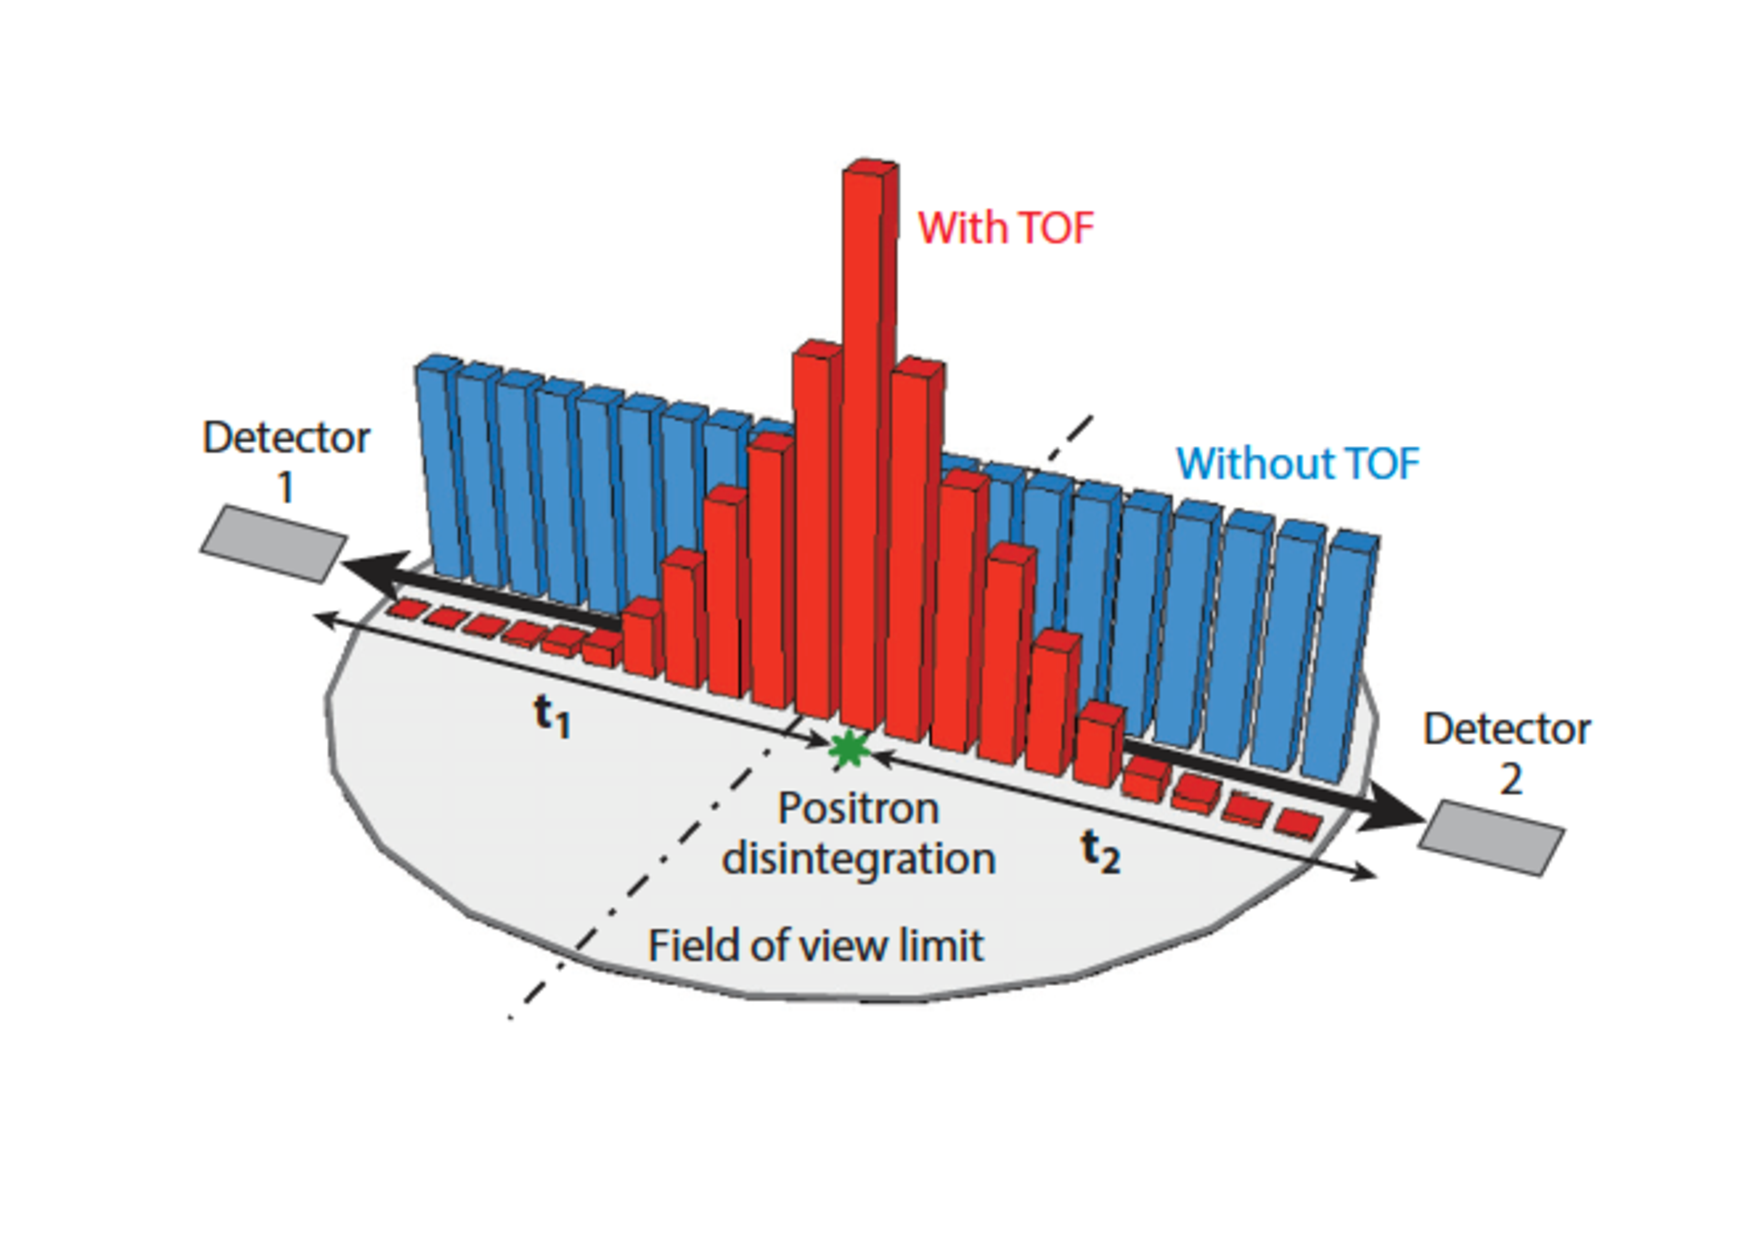
\includegraphics[width=0.8\textwidth]{03_GraphicFiles/chapter1_Introduction/PET_TOF.pdf}
%\caption{Schematic view of the information provided by \gls{tof} measurement to the \gls{pet} detection. Without \gls{tof}, a flat probability is assigned to the reconstructed \gls{lor} (blue), while the measurement of the arrival time difference between the two coincident photons is translated into a distance from the \gls{lor} midpoint where the probability density function should centered (red). In~\cite{Vaquero2015}.}
%\label{chap1::fig::NM_PET_TOF}
%\end{figure}   
%
%This possibility was explored already in the 1980s with fast scintillators~\parencite{Ter-Pogossian1982, Lewellen1988}, such as \gls{csf} and \gls{baf2}, which were anyway not adapted to clinical \gls{pet} application due to a low stopping power. On the other hand, the \gls{bgo} response was too slow to perform \gls{tof}. With the introduction of \gls{lso}, it was also recognized that its very good timing resolution (together with the one of the similar scintillator \gls{lyso}) could be utilized in the development of \gls{tof}-\gls{pet} systems~\parencite{Moses1999}, overcoming the limitation of the early designs of the 1980s. In 2005 Siemens presented the results from a prototype that achieved a timing resolution of 1.2~ns, and soon after the first \gls{tof}-\gls{pet} machine was launched by Philips (Philips Gemini TF)~\parencite{Karp2008}.  Based on \gls{lyso} crystal, it provided 585~ps system timing resolution. At present, all the main \gls{pet} vendors offer \gls{tof}-\gls{pet} solutions with hundreds of ps timing resolution. 
%Beyond PET detector designs using conventional \glspl{pm}, the arrival of \glspl{sipm} has led to a great interest in utilizing these new photosensors to achieve improved timing resolution in \gls{tof}-\gls{pet} scanners. Philips recently introduced the Vereos system, which uses digital  \glspl{sipm} for signal readout from individual \gls{lyso} crystals; such a machine provides a system coincidence timing resolution of approximately 310 ps~\parencite{Miller2015}. In parallel \gls{ge} developed the SIGNA \gls{tof}-\gls{pet}/\gls{mri} system using a detector ring based on analog \glspl{sipm} inserted in the magnet bore, thereby
%allowing simultaneous \gls{pet} and MR imaging. The reported system coincidence timing resolution of this system is 390–400~ps~\parencite{Levin2013}. Hence, while scanners with detectors using conventional \glspl{pm} are pushing closer to 400~ps timing resolution, new \gls{sipm} technology indicates that system resolution close to 300~ps is achievable with the lutetium based scintillators.
%With the rapid improvements of both scintillator and photosensor technology shown by recent results, a \gls{tof} resolution below 100~ps seems achievable in the next future~\parencite{Surti2016, Lecoq2017}.
%Recent studies also investigated cost-effective solutions to achieve performance comparable to present commercial systems. In particular, a whole-body \gls{pet} scanner based on plastic scintillators is being developed in Poland by the Jagiellonian University group. The J-PET is constructed with axially arranged strips of plastic scintillators, aiming to detect the annihilation photons via Compton interaction and read out on both sides by \glspl{pm}. The position of interaction in the scintillator is determined from the time difference of light signal arriving on each strip end. A \gls{tot} technique is used instead of the charge measurement of standard \gls{pet} systems in order to take advantage of the superior timing properties of plastic scintillators with respect to crystal detectors (\gls{lso} and \gls{bgo}). Preliminary studies showed that it is possible to achieve a coincidence time resolution of about 500~ps \gls{fwhm} with simple time measurements, coupled to a few millimeters spatial resolution~\parencite{Niedzwiecki2017}.
%
%\subsection{Single Photon Emission Computed Tomography}\label{chap1::subsec::SPECT_NM}
%In \gls{spect} tomographic images of the radionuclide distribution in the patient are generated from the emitted gamma photons detected as singles with collimated scintillators. Planar imaging reproduces a two-dimensional projection of the tracer distribution from a single view, while the tomographic image is obtained by the reconstruction of several slices collected from multiple camera positions. Both techniques are used in clinics: planar imaging is less demanding and only requires a single camera head, while multiple camera heads mounted on a rotating gantry are generally used for tomographic imaging, and image reconstruction is required.
%
%Although many innovations have been made since the introduction of the first gamma camera in 1958 by Hal Anger~\parencite{Anger1958}, today's clinical detectors share many of the essential features of Anger's early designs, and are often called Anger cameras. A standard \gls{spect} gamma camera is composed of an aperture or collimator which mechanically selects photons traveling in specific directions, depending on the collimator configuration. The photons approaching the camera from directions different than those specified by the collimation system are passively absorbed. The gamma photons with the selected direction then encounter a scintillation detectors coupled to photosensors. The related electronics and data acquisition system are generally optimized to impose energy threshold in order to reject undesired photons, such the ones which underwent scattering in the collimator section. A schematic view of the main component of the \gls{spect} camera is given in \figurename~\ref{chap1::fig::SPECT_components}, while a simplified view of the collimation principle is sketched in \figurename~\ref{chap1::fig::SPECT_collimator}.   
%
% \begin{figure}[!htbp]
%\begin{subfigure}[t]{.49\textwidth}
%\centering
%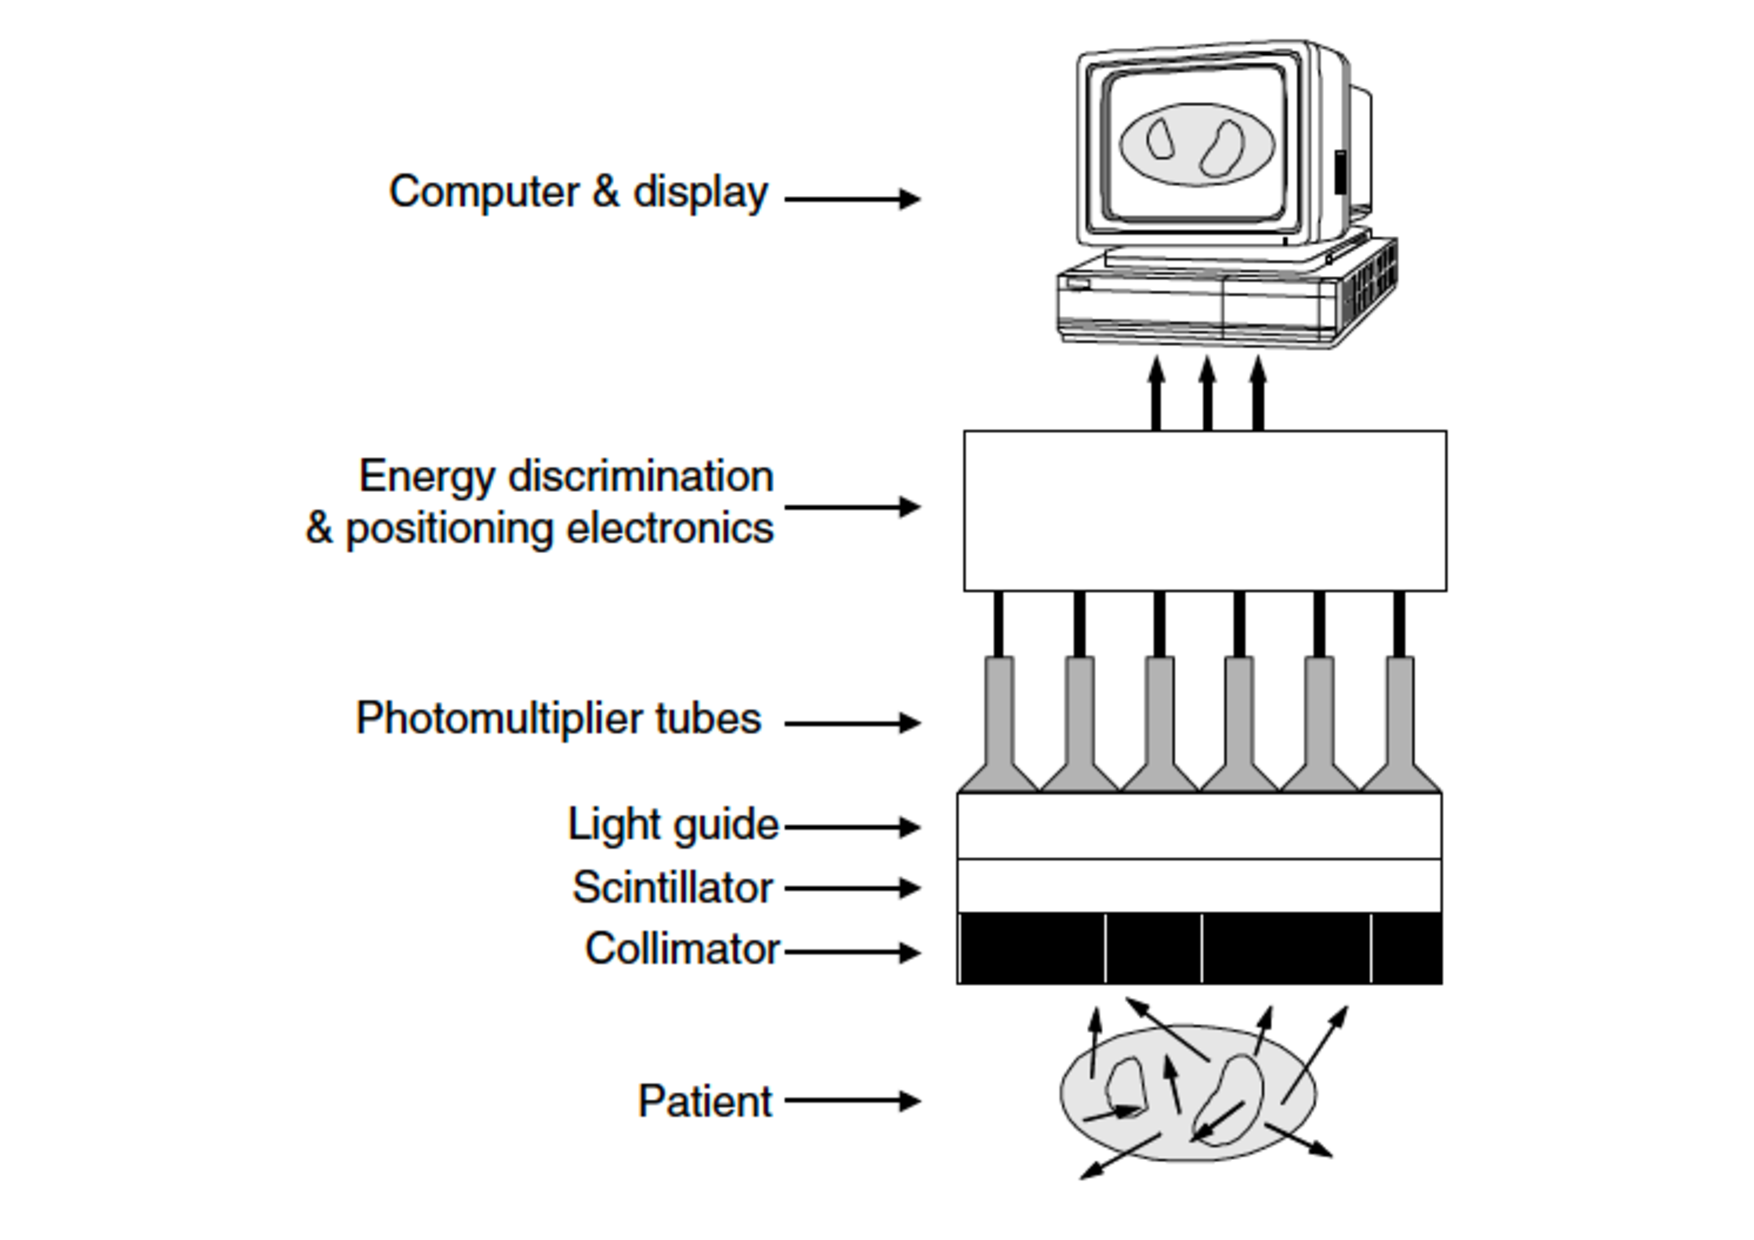
\includegraphics[width=0.7\linewidth]{03_GraphicFiles/chapter1_Introduction/SPECT_components.pdf}
%\caption{Schematic view of the main components of a \gls{spect} gamma camera.}
%\label{chap1::fig::SPECT_components}
%\end{subfigure}
%\begin{subfigure}[t]{.49\textwidth}
%\centering
%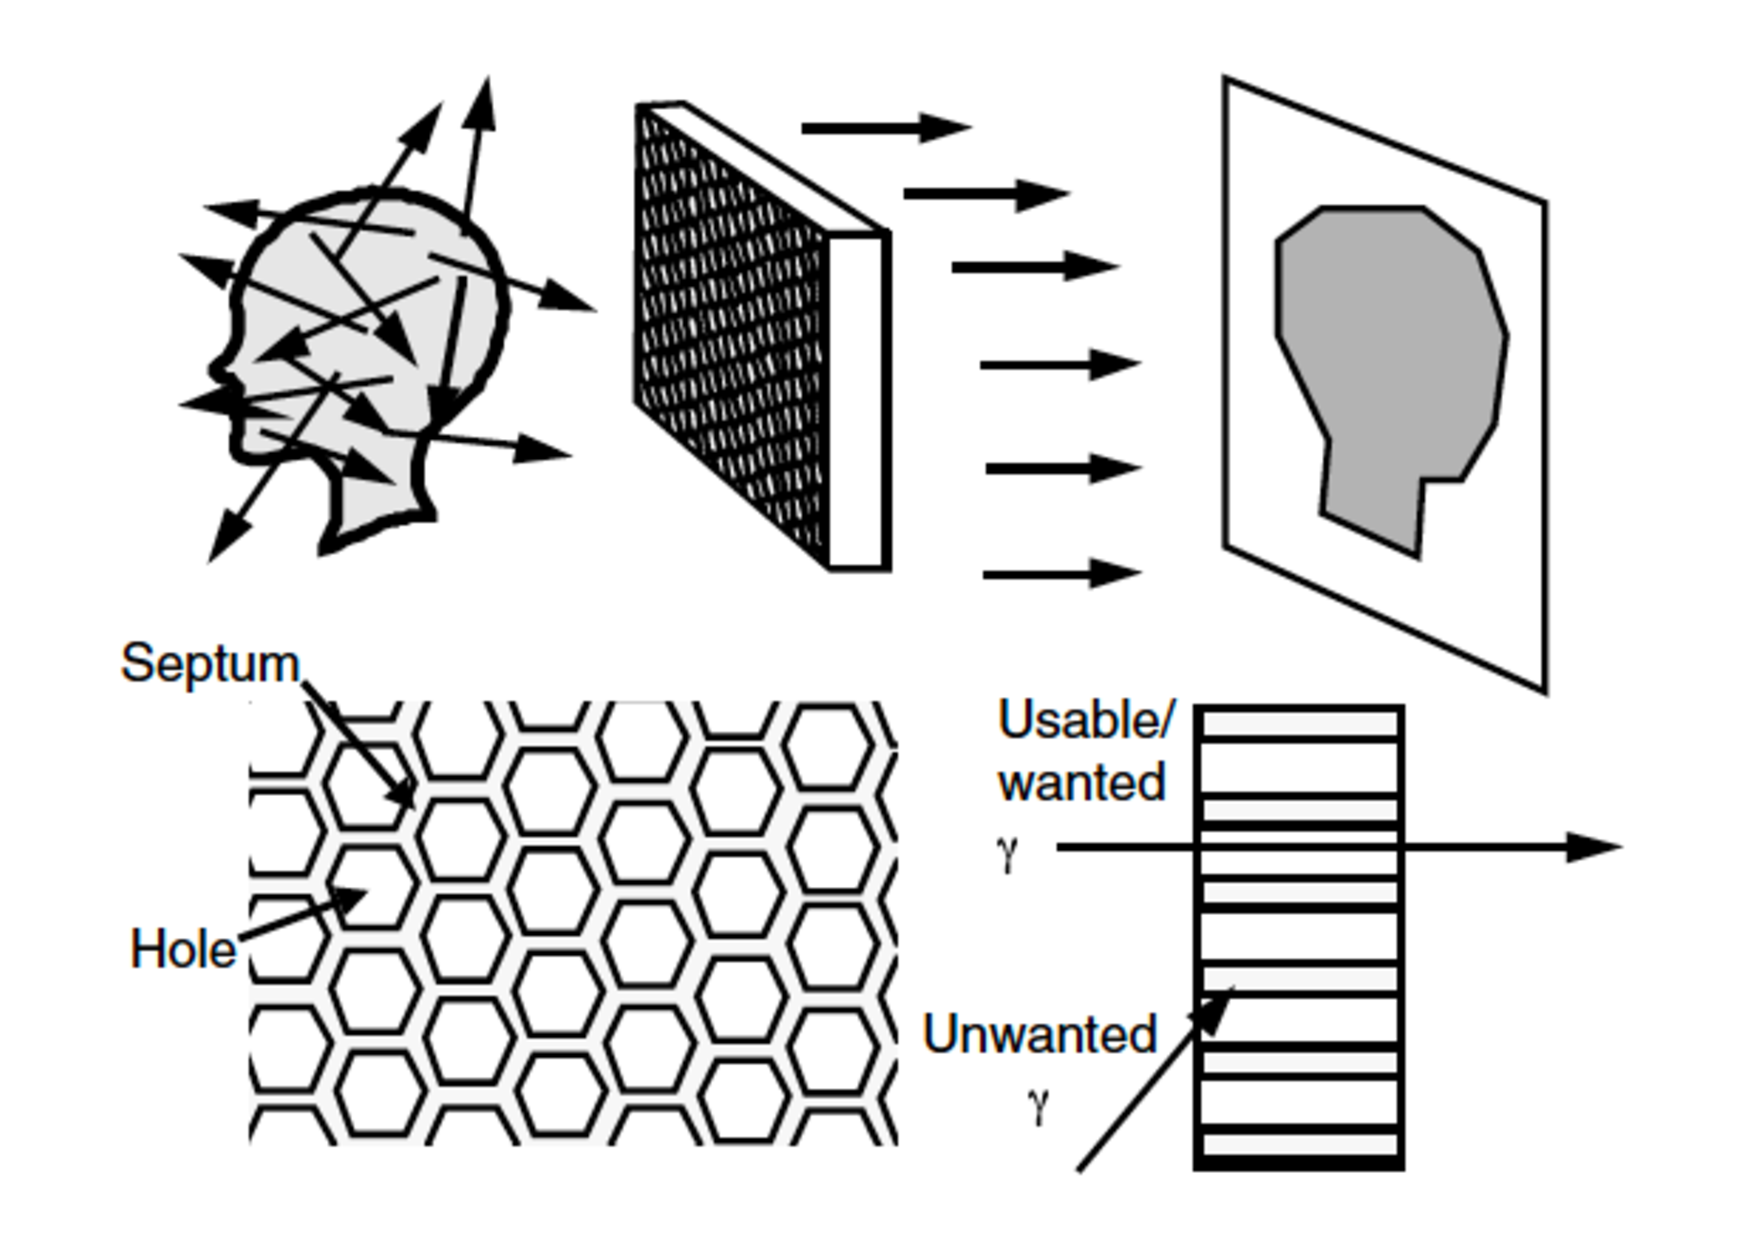
\includegraphics[width=0.98\linewidth]{03_GraphicFiles/chapter1_Introduction/SPECT_collimator.pdf}
%\caption{Schematic representation of the collimation principle of \gls{spect} gamma cameras.}
%\label{chap1::fig::SPECT_collimator}
%\end{subfigure}
%\caption{In~\cite{Zeng2004}.}
%\label{chap1::fig::SPECT_details}
%\end{figure} 
%
%The most simple photon passive selection device is the pinhole aperture, but acceptable spatial resolution can be only obtained at the expense of the system sensitivity. Improved, but always limited overall sensitivity is provided by the introduction of collimators, composed of array of holes separated by septa.  Collimator septa are composed of highly absorbing material with high atomic number and high density. Alloys of lead, tungsten and gold are the most common materials used for this purpose. 
%Various hole shapes (circular, square, triangular or hexagonal) are used in common collimators, but the hexagonal shape is the most diffused because it provides the best efficiency. In addition to parallel hole patterns, also converging and diverging collimators have been developed. Converging collimators magnify an image on a camera face and thus can yield finer resolution and/or higher sensitivity images than those resulting from used of parallel-hole collimators. Converging solutions are adapted to small-size objects with respect to the camera \gls{fov}, while the image of large object would result truncated (if part of the object is outside the \gls{fov} of the camera) or distorted (because the magnification is dependent on the distance from the collimator). 
%The most spread parallel-hole collimators find routine use in clinics in four configurations: \gls{lehr}, \gls{legp}, \gls{megp}, and \gls{hegp}. Each designation is adapted to a defined gamma energy range, and thus to certain radioisotopes, and is also an indication of the trade-off between resolution and sensitivity which are affected by the septal material, the hole size and length, and the septal thickness. Collimator sensitivity is maximized by the thinnest possible septa, but thin septa can lead to septal penetration which is extremely detrimental to diagnostic performance. The aforementioned trade-off is then a crucial parameter to be considered when designing a \gls{spect} camera, and, together with the employed scintillator and photosensor features, completely determine the overall system performance~\parencite{Gunter2004}.
%
%The origins of \gls{spect} imaging can be identified with the invention of the Anger scintillation camera in the late 1950s~\parencite{Anger1958, Anger1964}; previously, scans were performed by manually positioning a Geiger counter above the organ of interest, but with the Anger camera the entire organ could be scanned at one time. During the 1960s, both longitudinal and transaxial emission tomography were deeply studied. Crandall and Cassen developed a longitudinal tomographic scanner which used a highly focusing collimator placed on a large crystal-matrix detector~\parencite{Crandall1966}, and in 1969, Anger invented a sophisticated longitudinal tomograph that used a scanning scintillation camera~\parencite{Anger1969}. Transaxial tomographs were developed by Kuhl and colleagues between 1963 and 1976, and the final prototype used discrete scintillator arrays~\parencite{Kuhl1976}. Discrete scintillation detectors have been also used for other scanners in the late 1970s, but the first investigators to explore the possible implementation of an Anger camera for transaxial tomography were Paul Harper and colleagues at the University of Chicago. In the early stages, a rotatable chair was placed in fornt of a single head fixed Anger camera~\parencite{Muehllehner1971}. In 1976, Jaszczak and Keyes, independently developed a \gls{spect} system that used an Anger camera mounted on a rotating gantry~\parencite{Jaszczak1977, Keyes1977}. In the following years, the first whole-body \gls{spect} system was developed and clinically evaluated in 1978 at the Baylor College of Medicine~\parencite{Jaszczak1979}. During the late 1970s and the 1980s, both rotating-camera \gls{spect} systems and stationary detector configurations were proposed and developed in Europe and US~\parencite{Larsson1980, Rogers1988}, and the bases for modern machines were established. 
%The modern cameras, as mentioned, rely on the described designs and have been adapted.in the past years, to new tracers provided by the pharmaceutical industry. \gls{spect} takes advantage of many years of experience and is now a well-established imaging modality in nuclear medicine. Thanks to its cost-effectiveness, such an imaging technique is widely employed in the clinical routine, and all the major medical imaging companies offer a \gls{spect} system, generally in dual-head configuration with rotating gantry.
%At present, virtually all single-photon imaging in nuclear medicine relies on Anger-type cameras, relatively simple and cost-effective, but limited in sensitivity and energy acceptance given the presence of a mechanical photon selection system. Already in 1974 this limitation was addressed by Todd and Nightingale which proposed the application of Compton imaging method to nuclear medicine~\parencite{Todd1974}. The Compton detection principle is described in chapter~\ref{chap::2}. Starting from 1981, Singh and colleagues published a number of seminal papaers that described analytical and experimental results for Compton camera composed of a pixelated germanium first detector and a standard Anger camera as second detector~\parencite{Singh1981, Singh1983, Singh1983b}. The investigation of such an imaging modality for the application in single photon detection for nuclear medicine continued in the following year and is still today actively explored. In particular, the availability of new high-energy tracers could provide advantages in terms of dose and spatial accuracy, but high-energy photons are hardly collimated with mechanical passive system. The electronic collimation exploited by Compton cameras can be the solution for high-sensitivity and high-resolution \gls{spect} examinations. More details can be found in in chapter~\ref{chap::5} of this thesis, where the described topic has been addressed with simulation studies. The presented results have been recently published in~\parencite{Fontana2017_PMB} and~\parencite{Fontana2017_APPB}. 
%
%\subsection{Theranostics}\label{chap1::subsec::Theranostics}
%
%The theranostics approach in nuclear medicine couples diagnostic imaging and cancer therapy using the same molecule or at least very similar drugs, given in different dosages. For example, the combination of \gls{iod131} (gamma emitter) and \gls{lut177} (beta emitter), is used for both imaging and therapy. Furthermore, different isotopes of the same elements (for example \gls{iod123}, \gls{iod131} and the newer terbium isotopes - Tb) can also be used for theranostics given the multiple associated emission (beta and gamma, gamma rays at different energies, alpha and gamma)~\parencite{Gerard2002, Alzahrani2012, Muller2012}. During the treatment, theranostics can be applied in monitoring the therapy course and estimating the potential response and eventual toxicity. The safety of high cumulative doses of radioactive agents after multiple repeated cycles is, however, a cause of concern. Anyway, remarkable improvements have been obtained in targeted therapies, which have proven to be effective with favorable safety profiles~\parencite{Baum2012, Kwekkeboom2008, Strosberg2017}. The diagnostic part of theranostics can be performed with both \gls{pet} and \gls{spect} machines, depending on the employed radioisotope emissions. Most therapeutic radiopharmaceuticals are labeled with $\beta^{-}$-emitting isotopes, having a tissue penetration of only few millimeters and so adapted to spare the healthy tissues surrounding the tumor. The first theranostic radiopharmaceutical in nuclear medicine history was radioiodine, used for therapy and imaging in thyroid diseases~\parencite{Hertz2016}. iodine is taken up by the thyroid galnd for the production of hormones, vital for the development of the brain, normal growth and metabolic balance. In 19367, Hertz developed the idea of administrating radioactive iodine in patients with thyroid diseases, and few years of preclinical studies at the \gls{mit} (where the first cyclotron for medical use had been built) followed this first proposal. In 1941, the first patient was treated with radioiodine~\parencite{Hertz1942}. \gls{iod131} is to the date the gold standard for certain therapeutical indications, given its low cost and the advantageous combination of $\beta^{-}$ and gamma emission. The electron radiation targets the thyroid from the inside, while the organ can be visualized using a gamma camera.  
%
%Since its first proposal, the use of theranostic agents has been consistently increasing: the combination of targeted cancer imaging and therapy is a considerable contribution to personalized medicine and may play an important role in the future with the implementation of new chemical agents and the continuous improvement of imaging systems~\parencite{Yordanova2017}. For the peculiar context of this thesis it is worth to notice that, as for diagnosis \gls{spect}, high-energy gamma emitters can be applied in theranostics, and Compton camera can be implemented for the imaging task. This point is further discussed in chapter~\ref{chap::5}. 


\clearpage
%\printbibliography[heading=subbibintoc]
